\documentclass{article} % For LaTeX2e
\usepackage{style/iclr2023_conference,times}

% Optional math commands from https://github.com/goodfeli/dlbook_notation.
%%%%% NEW MATH DEFINITIONS %%%%%

\usepackage{amsmath,amsfonts,bm}

% Mark sections of captions for referring to divisions of figures
\newcommand{\figleft}{{\em (Left)}}
\newcommand{\figcenter}{{\em (Center)}}
\newcommand{\figright}{{\em (Right)}}
\newcommand{\figtop}{{\em (Top)}}
\newcommand{\figbottom}{{\em (Bottom)}}
\newcommand{\captiona}{{\em (a)}}
\newcommand{\captionb}{{\em (b)}}
\newcommand{\captionc}{{\em (c)}}
\newcommand{\captiond}{{\em (d)}}

% Highlight a newly defined term
\newcommand{\newterm}[1]{{\bf #1}}


% Figure reference, lower-case.
\def\figref#1{figure~\ref{#1}}
% Figure reference, capital. For start of sentence
\def\Figref#1{Figure~\ref{#1}}
\def\twofigref#1#2{figures \ref{#1} and \ref{#2}}
\def\quadfigref#1#2#3#4{figures \ref{#1}, \ref{#2}, \ref{#3} and \ref{#4}}
% Section reference, lower-case.
\def\secref#1{section~\ref{#1}}
% Section reference, capital.
\def\Secref#1{Section~\ref{#1}}
% Reference to two sections.
\def\twosecrefs#1#2{sections \ref{#1} and \ref{#2}}
% Reference to three sections.
\def\secrefs#1#2#3{sections \ref{#1}, \ref{#2} and \ref{#3}}
% Reference to an equation, lower-case.
\def\eqref#1{equation~\ref{#1}}
% Reference to an equation, upper case
\def\Eqref#1{Equation~\ref{#1}}
% A raw reference to an equation---avoid using if possible
\def\plaineqref#1{\ref{#1}}
% Reference to a chapter, lower-case.
\def\chapref#1{chapter~\ref{#1}}
% Reference to an equation, upper case.
\def\Chapref#1{Chapter~\ref{#1}}
% Reference to a range of chapters
\def\rangechapref#1#2{chapters\ref{#1}--\ref{#2}}
% Reference to an algorithm, lower-case.
\def\algref#1{algorithm~\ref{#1}}
% Reference to an algorithm, upper case.
\def\Algref#1{Algorithm~\ref{#1}}
\def\twoalgref#1#2{algorithms \ref{#1} and \ref{#2}}
\def\Twoalgref#1#2{Algorithms \ref{#1} and \ref{#2}}
% Reference to a part, lower case
\def\partref#1{part~\ref{#1}}
% Reference to a part, upper case
\def\Partref#1{Part~\ref{#1}}
\def\twopartref#1#2{parts \ref{#1} and \ref{#2}}

\def\ceil#1{\lceil #1 \rceil}
\def\floor#1{\lfloor #1 \rfloor}
\def\1{\bm{1}}
\newcommand{\train}{\mathcal{D}}
\newcommand{\valid}{\mathcal{D_{\mathrm{valid}}}}
\newcommand{\test}{\mathcal{D_{\mathrm{test}}}}

\def\eps{{\epsilon}}


% Random variables
\def\reta{{\textnormal{$\eta$}}}
\def\ra{{\textnormal{a}}}
\def\rb{{\textnormal{b}}}
\def\rc{{\textnormal{c}}}
\def\rd{{\textnormal{d}}}
\def\re{{\textnormal{e}}}
\def\rf{{\textnormal{f}}}
\def\rg{{\textnormal{g}}}
\def\rh{{\textnormal{h}}}
\def\ri{{\textnormal{i}}}
\def\rj{{\textnormal{j}}}
\def\rk{{\textnormal{k}}}
\def\rl{{\textnormal{l}}}
% rm is already a command, just don't name any random variables m
\def\rn{{\textnormal{n}}}
\def\ro{{\textnormal{o}}}
\def\rp{{\textnormal{p}}}
\def\rq{{\textnormal{q}}}
\def\rr{{\textnormal{r}}}
\def\rs{{\textnormal{s}}}
\def\rt{{\textnormal{t}}}
\def\ru{{\textnormal{u}}}
\def\rv{{\textnormal{v}}}
\def\rw{{\textnormal{w}}}
\def\rx{{\textnormal{x}}}
\def\ry{{\textnormal{y}}}
\def\rz{{\textnormal{z}}}

% Random vectors
\def\rvepsilon{{\mathbf{\epsilon}}}
\def\rvtheta{{\mathbf{\theta}}}
\def\rva{{\mathbf{a}}}
\def\rvb{{\mathbf{b}}}
\def\rvc{{\mathbf{c}}}
\def\rvd{{\mathbf{d}}}
\def\rve{{\mathbf{e}}}
\def\rvf{{\mathbf{f}}}
\def\rvg{{\mathbf{g}}}
\def\rvh{{\mathbf{h}}}
\def\rvu{{\mathbf{i}}}
\def\rvj{{\mathbf{j}}}
\def\rvk{{\mathbf{k}}}
\def\rvl{{\mathbf{l}}}
\def\rvm{{\mathbf{m}}}
\def\rvn{{\mathbf{n}}}
\def\rvo{{\mathbf{o}}}
\def\rvp{{\mathbf{p}}}
\def\rvq{{\mathbf{q}}}
\def\rvr{{\mathbf{r}}}
\def\rvs{{\mathbf{s}}}
\def\rvt{{\mathbf{t}}}
\def\rvu{{\mathbf{u}}}
\def\rvv{{\mathbf{v}}}
\def\rvw{{\mathbf{w}}}
\def\rvx{{\mathbf{x}}}
\def\rvy{{\mathbf{y}}}
\def\rvz{{\mathbf{z}}}

% Elements of random vectors
\def\erva{{\textnormal{a}}}
\def\ervb{{\textnormal{b}}}
\def\ervc{{\textnormal{c}}}
\def\ervd{{\textnormal{d}}}
\def\erve{{\textnormal{e}}}
\def\ervf{{\textnormal{f}}}
\def\ervg{{\textnormal{g}}}
\def\ervh{{\textnormal{h}}}
\def\ervi{{\textnormal{i}}}
\def\ervj{{\textnormal{j}}}
\def\ervk{{\textnormal{k}}}
\def\ervl{{\textnormal{l}}}
\def\ervm{{\textnormal{m}}}
\def\ervn{{\textnormal{n}}}
\def\ervo{{\textnormal{o}}}
\def\ervp{{\textnormal{p}}}
\def\ervq{{\textnormal{q}}}
\def\ervr{{\textnormal{r}}}
\def\ervs{{\textnormal{s}}}
\def\ervt{{\textnormal{t}}}
\def\ervu{{\textnormal{u}}}
\def\ervv{{\textnormal{v}}}
\def\ervw{{\textnormal{w}}}
\def\ervx{{\textnormal{x}}}
\def\ervy{{\textnormal{y}}}
\def\ervz{{\textnormal{z}}}

% Random matrices
\def\rmA{{\mathbf{A}}}
\def\rmB{{\mathbf{B}}}
\def\rmC{{\mathbf{C}}}
\def\rmD{{\mathbf{D}}}
\def\rmE{{\mathbf{E}}}
\def\rmF{{\mathbf{F}}}
\def\rmG{{\mathbf{G}}}
\def\rmH{{\mathbf{H}}}
\def\rmI{{\mathbf{I}}}
\def\rmJ{{\mathbf{J}}}
\def\rmK{{\mathbf{K}}}
\def\rmL{{\mathbf{L}}}
\def\rmM{{\mathbf{M}}}
\def\rmN{{\mathbf{N}}}
\def\rmO{{\mathbf{O}}}
\def\rmP{{\mathbf{P}}}
\def\rmQ{{\mathbf{Q}}}
\def\rmR{{\mathbf{R}}}
\def\rmS{{\mathbf{S}}}
\def\rmT{{\mathbf{T}}}
\def\rmU{{\mathbf{U}}}
\def\rmV{{\mathbf{V}}}
\def\rmW{{\mathbf{W}}}
\def\rmX{{\mathbf{X}}}
\def\rmY{{\mathbf{Y}}}
\def\rmZ{{\mathbf{Z}}}

% Elements of random matrices
\def\ermA{{\textnormal{A}}}
\def\ermB{{\textnormal{B}}}
\def\ermC{{\textnormal{C}}}
\def\ermD{{\textnormal{D}}}
\def\ermE{{\textnormal{E}}}
\def\ermF{{\textnormal{F}}}
\def\ermG{{\textnormal{G}}}
\def\ermH{{\textnormal{H}}}
\def\ermI{{\textnormal{I}}}
\def\ermJ{{\textnormal{J}}}
\def\ermK{{\textnormal{K}}}
\def\ermL{{\textnormal{L}}}
\def\ermM{{\textnormal{M}}}
\def\ermN{{\textnormal{N}}}
\def\ermO{{\textnormal{O}}}
\def\ermP{{\textnormal{P}}}
\def\ermQ{{\textnormal{Q}}}
\def\ermR{{\textnormal{R}}}
\def\ermS{{\textnormal{S}}}
\def\ermT{{\textnormal{T}}}
\def\ermU{{\textnormal{U}}}
\def\ermV{{\textnormal{V}}}
\def\ermW{{\textnormal{W}}}
\def\ermX{{\textnormal{X}}}
\def\ermY{{\textnormal{Y}}}
\def\ermZ{{\textnormal{Z}}}

% Vectors
\def\vzero{{\bm{0}}}
\def\vone{{\bm{1}}}
\def\vmu{{\bm{\mu}}}
\def\vtheta{{\bm{\theta}}}
\def\vpsi{{\bm{\psi}}}
\def\vsigma{{\bm{\sigma}}}
\def\vlambda{{\bm{\lambda}}}
\def\vgamma{{\bm{\gamma}}}
\def\vomega{{\bm{\omega}}}
\def\va{{\bm{a}}}
\def\vb{{\bm{b}}}
\def\vc{{\bm{c}}}
\def\vd{{\bm{d}}}
\def\ve{{\bm{e}}}
\def\vf{{\bm{f}}}
\def\vg{{\bm{g}}}
\def\vh{{\bm{h}}}
\def\vi{{\bm{i}}}
\def\vj{{\bm{j}}}
\def\vk{{\bm{k}}}
\def\vl{{\bm{l}}}
\def\vm{{\bm{m}}}
\def\vn{{\bm{n}}}
\def\vo{{\bm{o}}}
\def\vp{{\bm{p}}}
\def\vq{{\bm{q}}}
\def\vr{{\bm{r}}}
\def\vs{{\bm{s}}}
\def\vt{{\bm{t}}}
\def\vu{{\bm{u}}}
\def\vv{{\bm{v}}}
\def\vw{{\bm{w}}}
\def\vx{{\bm{x}}}
\def\vy{{\bm{y}}}
\def\vz{{\bm{z}}}

% Elements of vectors
\def\evalpha{{\alpha}}
\def\evbeta{{\beta}}
\def\evepsilon{{\epsilon}}
\def\evlambda{{\lambda}}
\def\evomega{{\omega}}
\def\evmu{{\mu}}
\def\evpsi{{\psi}}
\def\evsigma{{\sigma}}
\def\evtheta{{\theta}}
\def\evgamma{{\gamma}}
\def\eva{{a}}
\def\evb{{b}}
\def\evc{{c}}
\def\evd{{d}}
\def\eve{{e}}
\def\evf{{f}}
\def\evg{{g}}
\def\evh{{h}}
\def\evi{{i}}
\def\evj{{j}}
\def\evk{{k}}
\def\evl{{l}}
\def\evm{{m}}
\def\evn{{n}}
\def\evo{{o}}
\def\evp{{p}}
\def\evq{{q}}
\def\evr{{r}}
\def\evs{{s}}
\def\evt{{t}}
\def\evu{{u}}
\def\evv{{v}}
\def\evw{{w}}
\def\evx{{x}}
\def\evy{{y}}
\def\evz{{z}}

% Matrix
\def\mA{{\bm{A}}}
\def\mB{{\bm{B}}}
\def\mC{{\bm{C}}}
\def\mD{{\bm{D}}}
\def\mE{{\bm{E}}}
\def\mF{{\bm{F}}}
\def\mG{{\bm{G}}}
\def\mH{{\bm{H}}}
\def\mI{{\bm{I}}}
\def\mJ{{\bm{J}}}
\def\mK{{\bm{K}}}
\def\mL{{\bm{L}}}
\def\mM{{\bm{M}}}
\def\mN{{\bm{N}}}
\def\mO{{\bm{O}}}
\def\mP{{\bm{P}}}
\def\mQ{{\bm{Q}}}
\def\mR{{\bm{R}}}
\def\mS{{\bm{S}}}
\def\mT{{\bm{T}}}
\def\mU{{\bm{U}}}
\def\mV{{\bm{V}}}
\def\mW{{\bm{W}}}
\def\mX{{\bm{X}}}
\def\mY{{\bm{Y}}}
\def\mZ{{\bm{Z}}}
\def\mBeta{{\bm{\beta}}}
\def\mPhi{{\bm{\Phi}}}
\def\mPsi{{\bm{\Psi}}}
\def\mTheta{{\bm{\Theta}}}
\def\mLambda{{\bm{\Lambda}}}
\def\mSigma{{\bm{\Sigma}}}

% Tensor
\DeclareMathAlphabet{\mathsfit}{\encodingdefault}{\sfdefault}{m}{sl}
\SetMathAlphabet{\mathsfit}{bold}{\encodingdefault}{\sfdefault}{bx}{n}
\newcommand{\tens}[1]{\bm{\mathsfit{#1}}}
\def\tA{{\tens{A}}}
\def\tB{{\tens{B}}}
\def\tC{{\tens{C}}}
\def\tD{{\tens{D}}}
\def\tE{{\tens{E}}}
\def\tF{{\tens{F}}}
\def\tG{{\tens{G}}}
\def\tH{{\tens{H}}}
\def\tI{{\tens{I}}}
\def\tJ{{\tens{J}}}
\def\tK{{\tens{K}}}
\def\tL{{\tens{L}}}
\def\tM{{\tens{M}}}
\def\tN{{\tens{N}}}
\def\tO{{\tens{O}}}
\def\tP{{\tens{P}}}
\def\tQ{{\tens{Q}}}
\def\tR{{\tens{R}}}
\def\tS{{\tens{S}}}
\def\tT{{\tens{T}}}
\def\tU{{\tens{U}}}
\def\tV{{\tens{V}}}
\def\tW{{\tens{W}}}
\def\tX{{\tens{X}}}
\def\tY{{\tens{Y}}}
\def\tZ{{\tens{Z}}}


% Graph
\def\gA{{\mathcal{A}}}
\def\gB{{\mathcal{B}}}
\def\gC{{\mathcal{C}}}
\def\gD{{\mathcal{D}}}
\def\gE{{\mathcal{E}}}
\def\gF{{\mathcal{F}}}
\def\gG{{\mathcal{G}}}
\def\gH{{\mathcal{H}}}
\def\gI{{\mathcal{I}}}
\def\gJ{{\mathcal{J}}}
\def\gK{{\mathcal{K}}}
\def\gL{{\mathcal{L}}}
\def\gM{{\mathcal{M}}}
\def\gN{{\mathcal{N}}}
\def\gO{{\mathcal{O}}}
\def\gP{{\mathcal{P}}}
\def\gQ{{\mathcal{Q}}}
\def\gR{{\mathcal{R}}}
\def\gS{{\mathcal{S}}}
\def\gT{{\mathcal{T}}}
\def\gU{{\mathcal{U}}}
\def\gV{{\mathcal{V}}}
\def\gW{{\mathcal{W}}}
\def\gX{{\mathcal{X}}}
\def\gY{{\mathcal{Y}}}
\def\gZ{{\mathcal{Z}}}

% Sets
\def\sA{{\mathbb{A}}}
\def\sB{{\mathbb{B}}}
\def\sC{{\mathbb{C}}}
\def\sD{{\mathbb{D}}}
% Don't use a set called E, because this would be the same as our symbol
% for expectation.
\def\sF{{\mathbb{F}}}
\def\sG{{\mathbb{G}}}
\def\sH{{\mathbb{H}}}
\def\sI{{\mathbb{I}}}
\def\sJ{{\mathbb{J}}}
\def\sK{{\mathbb{K}}}
\def\sL{{\mathbb{L}}}
\def\sM{{\mathbb{M}}}
\def\sN{{\mathbb{N}}}
\def\sO{{\mathbb{O}}}
\def\sP{{\mathbb{P}}}
\def\sQ{{\mathbb{Q}}}
\def\sR{{\mathbb{R}}}
\def\sS{{\mathbb{S}}}
\def\sT{{\mathbb{T}}}
\def\sU{{\mathbb{U}}}
\def\sV{{\mathbb{V}}}
\def\sW{{\mathbb{W}}}
\def\sX{{\mathbb{X}}}
\def\sY{{\mathbb{Y}}}
\def\sZ{{\mathbb{Z}}}

% Entries of a matrix
\def\emLambda{{\Lambda}}
\def\emA{{A}}
\def\emB{{B}}
\def\emC{{C}}
\def\emD{{D}}
\def\emE{{E}}
\def\emF{{F}}
\def\emG{{G}}
\def\emH{{H}}
\def\emI{{I}}
\def\emJ{{J}}
\def\emK{{K}}
\def\emL{{L}}
\def\emM{{M}}
\def\emN{{N}}
\def\emO{{O}}
\def\emP{{P}}
\def\emQ{{Q}}
\def\emR{{R}}
\def\emS{{S}}
\def\emT{{T}}
\def\emU{{U}}
\def\emV{{V}}
\def\emW{{W}}
\def\emX{{X}}
\def\emY{{Y}}
\def\emZ{{Z}}
\def\emSigma{{\Sigma}}
\def\emPhi{{\Phi}}
\def\emPsi{{\Psi}}
\def\emTheta{{\Theta}}




% entries of a tensor
% Same font as tensor, without \bm wrapper
\newcommand{\etens}[1]{\mathsfit{#1}}
\def\etLambda{{\etens{\Lambda}}}
\def\etA{{\etens{A}}}
\def\etB{{\etens{B}}}
\def\etC{{\etens{C}}}
\def\etD{{\etens{D}}}
\def\etE{{\etens{E}}}
\def\etF{{\etens{F}}}
\def\etG{{\etens{G}}}
\def\etH{{\etens{H}}}
\def\etI{{\etens{I}}}
\def\etJ{{\etens{J}}}
\def\etK{{\etens{K}}}
\def\etL{{\etens{L}}}
\def\etM{{\etens{M}}}
\def\etN{{\etens{N}}}
\def\etO{{\etens{O}}}
\def\etP{{\etens{P}}}
\def\etQ{{\etens{Q}}}
\def\etR{{\etens{R}}}
\def\etS{{\etens{S}}}
\def\etT{{\etens{T}}}
\def\etU{{\etens{U}}}
\def\etV{{\etens{V}}}
\def\etW{{\etens{W}}}
\def\etX{{\etens{X}}}
\def\etY{{\etens{Y}}}
\def\etZ{{\etens{Z}}}

% The true underlying data generating distribution
\newcommand{\pdata}{p_{\rm{data}}}
% The empirical distribution defined by the training set
\newcommand{\ptrain}{\hat{p}_{\rm{data}}}
\newcommand{\Ptrain}{\hat{P}_{\rm{data}}}
% The model distribution
\newcommand{\pmodel}{p_{\rm{model}}}
\newcommand{\Pmodel}{P_{\rm{model}}}
\newcommand{\ptildemodel}{\tilde{p}_{\rm{model}}}
% Stochastic autoencoder distributions
\newcommand{\pencode}{p_{\rm{encoder}}}
\newcommand{\pdecode}{p_{\rm{decoder}}}
\newcommand{\precons}{p_{\rm{reconstruct}}}

\newcommand{\laplace}{\mathrm{Laplace}} % Laplace distribution

\newcommand{\E}{\mathbb{E}}
\newcommand{\Ls}{\mathcal{L}}
\newcommand{\R}{\mathbb{R}}
\newcommand{\emp}{\tilde{p}}
\newcommand{\lr}{\alpha}
\newcommand{\reg}{\lambda}
\newcommand{\rect}{\mathrm{rectifier}}
\newcommand{\softmax}{\mathrm{softmax}}
\newcommand{\sigmoid}{\sigma}
\newcommand{\softplus}{\zeta}
\newcommand{\KL}{D_{\mathrm{KL}}}
\newcommand{\Var}{\mathrm{Var}}
\newcommand{\standarderror}{\mathrm{SE}}
\newcommand{\Cov}{\mathrm{Cov}}
% Wolfram Mathworld says $L^2$ is for function spaces and $\ell^2$ is for vectors
% But then they seem to use $L^2$ for vectors throughout the site, and so does
% wikipedia.
\newcommand{\normlzero}{L^0}
\newcommand{\normlone}{L^1}
\newcommand{\normltwo}{L^2}
\newcommand{\normlp}{L^p}
\newcommand{\normmax}{L^\infty}

\newcommand{\parents}{Pa} % See usage in notation.tex. Chosen to match Daphne's book.

\DeclareMathOperator*{\argmax}{arg\,max}
\DeclareMathOperator*{\argmin}{arg\,min}

\DeclareMathOperator{\sign}{sign}
\DeclareMathOperator{\Tr}{Tr}
\let\ab\allowbreak


\usepackage{url}

% Additional stuff

\usepackage{titletoc}
\usepackage{hyperref}

\usepackage{graphicx}
\usepackage{mathtools}
\usepackage{amssymb}
\usepackage{amsthm}
\usepackage[nameinlink,capitalize]{cleveref}
\usepackage{makecell}
\usepackage{pgfplots}
\usepackage{subcaption}
\usepackage{siunitx}
\usepackage{wrapfig}
\usepackage{booktabs}

% THEOREMS
\theoremstyle{plain}
\newtheorem{theorem}{Theorem}[section]
\newtheorem{proposition}[theorem]{Proposition}
\newtheorem{lemma}[theorem]{Lemma}
\newtheorem{corollary}[theorem]{Corollary}
\theoremstyle{definition}
\newtheorem{definition}[theorem]{Definition}
\newtheorem{assumption}[theorem]{Assumption}
\theoremstyle{remark}
\newtheorem{remark}[theorem]{Remark}


\newtheorem{innercustomthm}{Theorem}
\newenvironment{customthm}[1]
{\renewcommand\theinnercustomthm{#1}\innercustomthm}
{\endinnercustomthm}

% AUTOREF
\renewcommand*{\figureautorefname}{Fig.}
\renewcommand*{\equationautorefname}{Eq.}
\renewcommand{\sectionautorefname}{§}
\renewcommand*{\subsectionautorefname}{\sectionautorefname}
\renewcommand*{\subsubsectionautorefname}{\sectionautorefname}
\renewcommand{\appendixautorefname}{\sectionautorefname}
\newcommand{\lemmaautorefname}{Lemma}
\newcommand{\propositionautorefname}{Proposition}
\newcommand{\definitionautorefname}{Definition}
\newcommand{\innercustomthmautorefname}{Theorem}
\newcommand{\innercustompropautorefname}{Proposition}
\crefname{definition}{Definition}{Definitions}

\title{Localized Randomized Smoothing\\for Collective Robustness Certification}

% Authors must not appear in the submitted version. They should be hidden
% as long as the \iclrfinalcopy macro remains commented out below.
% Non-anonymous submissions will be rejected without review.

\author{Jan Schuchardt$^{1}$\thanks{equal contribution}~, ~Tom Wollschl\"ager$^{1 \fnsymbol{footnote}}$, ~Aleksandar Bojchevski$^{2}$, ~Stephan G\"unnemann$^{1}$\\
\texttt{\{j.schuchardt,t.wollschlaeger,s.guennemann\}@tum.de}\\
\texttt{\{bojchevski\}@cispa.de} \\
\textsuperscript{1}Technical University of Munich \\
\textsuperscript{2}CISPA Helmholtz Center for Information Security \\
}

\iffalse
\author{Jan Schuchardt, Tom Wollschläger, Aleksandar Bojchevski \thanks{ Use footnote for providing further information
about author (webpage, alternative address)---\emph{not} for acknowledging
funding agencies.  Funding acknowledgements go at the end of the paper.} \\
Department of Computer Science\\
Cranberry-Lemon University\\
Pittsburgh, PA 15213, USA \\
\texttt{\{hippo,brain,jen\}@cs.cranberry-lemon.edu} \\
\And
Ji Q. Ren \& Yevgeny LeNet \\
Department of Computational Neuroscience \\
University of the Witwatersrand \\
Joburg, South Africa \\
\texttt{\{robot,net\}@wits.ac.za} \\
\AND
Coauthor \\
Affiliation \\
Address \\
\texttt{email}
}
\fi

% The \author macro works with any number of authors. There are two commands
% used to separate the names and addresses of multiple authors: \And and \AND.
%
% Using \And between authors leaves it to \LaTeX{} to determine where to break
% the lines. Using \AND forces a linebreak at that point. So, if \LaTeX{}
% puts 3 of 4 authors names on the first line, and the last on the second
% line, try using \AND instead of \And before the third author name.

\newcommand{\fix}{\marginpar{FIX}}
\newcommand{\new}{\marginpar{NEW}}

\iclrfinalcopy % Uncomment for camera-ready version, but NOT for submission.
\begin{document}


\maketitle

\begin{abstract}
Models for image segmentation, node classification and many other tasks map a single input to multiple labels.
By perturbing this single shared input (e.g.~the image) an adversary can manipulate several predictions (e.g.~misclassify several pixels).
Collective robustness certification is the task of provably bounding the number of robust predictions under this threat model.
The only dedicated method that goes beyond certifying each output independently is limited to \textit{strictly local} models, where each prediction is associated with a small receptive field.
We propose a more general collective robustness certificate for all types of models. We further show that this approach is beneficial for the larger class of \textit{softly local} models, where each output is dependent on the entire input
but assigns different levels of importance to different input regions (e.g.~based on their proximity in the image).
The certificate is based on our novel localized randomized smoothing approach, where the random perturbation strength for different input regions is proportional to their importance for the outputs.
%The resulting locally smoothed model yields strong collective guarantees while maintaining high prediction quality on both image segmentation and node classification tasks.
Localized smoothing Pareto-dominates existing certificates on both image segmentation and node classification tasks, simultaneously offering higher accuracy and stronger certificates.
\end{abstract}

\section{Introduction}\label{section:introduction}
There is a wide range of tasks that require models making multiple predictions based on a single input.
For example,  semantic segmentation  requires assigning a label to each pixel in an image.
When deploying such \textit{multi-output} classifiers in practice, their robustness should be a key concern.
After all -- just like simple classifiers \citep{Szegedy2014} -- they can fall victim to adversarial attacks \citep{Xie2017, Zuegner2018,  Belinkov2018}. Even without an adversary, random noise or measuring errors can cause predictions to unexpectedly change.

We propose a novel method providing provable guarantees on \textit{how many} predictions can be changed by an adversary.
As all outputs operate on the same input, they have to be attacked simultaneously by choosing a single perturbed input,
which can be more challenging for an adversary than attacking them independently.
We must account for this to obtain a proper \textit{collective robustness certificate}.

The only dedicated collective certificate that goes beyond certifying each output independently~\citep{Schuchardt2021} is only beneficial for models we call \textit{strictly local}, where each output depends  on a small, pre-defined subset of the input. 
Multi-output classifiers
%used in practic
, however, are often only \textit{softly local}.
While all
%of 
their predictions are in principle dependent on the entire input, each output may assign different importance to different subsets.
For example, convolutional networks for image segmentation can have small effective receptive fields \citep{Luo2016,Liu2018}, i.e.\ primarily use a small region of the image in labeling each pixel.
Many models for node classification are based on the homophily assumption that connected nodes are mostly of the same class. Thus, they primarily use features from neighboring nodes.
Transformers, which can in principle attend to arbitrary parts of the input, may in practice learn ``sparse'' attention maps, with the prediction for each token being mostly determined by a few (not necessarily nearby) tokens \citep{Shi2021}.
\begin{figure}
	\centering
	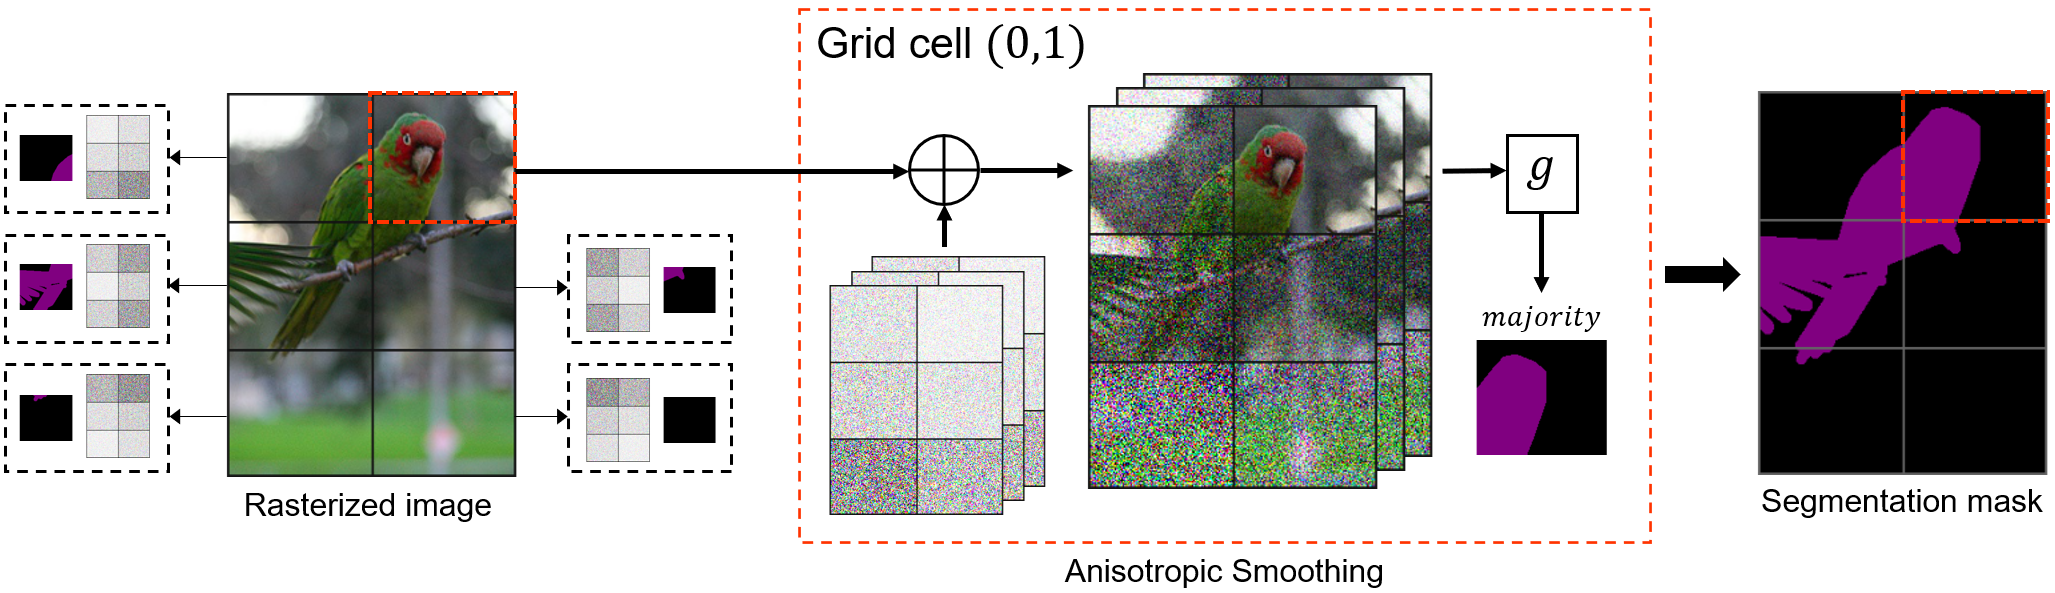
\includegraphics[width=\columnwidth]{figures/main_figure_new.png}
	\caption{Localized randomized smoothing applied to semantic segmentation.
		We assume that the most relevant information for labeling a pixel is contained in other nearby pixels.
		We partition the input image into multiple grid cells.
		For each grid cell, we sample noisy images from a \textit{different} anisotropic distribution that applies more noise to far-away, less relevant 
		cells.
		Segmenting all noisy images, cropping the result and computing the majority vote %(i.e.~the most common label for each pixel)
		yields a local segmentation mask.
		These per-cell segmentation masks can then be combined into a complete segmentation mask.}
	\label{fig:main_figure}
	\vskip-0.2in
\end{figure}

Softly local models pose a \textit{budget allocation problem} for
an adversary that tries to simultaneously manipulate multiple predictions by crafting a single perturbed input.
When each output is primarily focused on a different part of the input, the attacker has to distribute their limited adversarial budget and may be unable to attack all predictions at once.

We propose \textit{localized randomized smoothing}, a novel method for the collective robustness certification of softly local models that exploits this budget allocation problem.
%Randomized smoothing \citep{Liu2018b, Lecuyer2019, Cohen2019} is a versatile black-box certification method. Instead of directly analysing a model, it constructs a smoothed classifier that returns the expected prediction of the model under random perturbations of its input. This smoothed classifier can then be efficiently certified using statistical methods (more details in \autoref{section:background}). Randomized smoothing is typically applied to single-output models with isotropic Gaussian noise.
%Our localized randomized smoothing approach, however, 
It is an extension of randomized smoothing \citep{Lecuyer2019,Li2019,Cohen2019}, a versatile black-box certification method which is based on constructing a smoothed classifier that returns the expected prediction of a model under random perturbations of its input (more details in \autoref{section:background}).
Randomized smoothing is typically applied to single-output models with \textit{isotropic} Gaussian noise.
In localized smoothing however, we smooth each output (or set of outputs) of a multi-output classifier using a \textit{different}
distribution that is \textit{anisotropic}.
This is illustrated in \autoref{fig:main_figure}, where the predicted segmentation masks for each grid cell are smoothed using a different distribution.
%that applies more noise to farther away cells.
For instance, the distribution for segmenting the top-right cell applies less noise to the top-right cell.
The smoothing distribution for segmenting the bottom-left cell applies significantly more noise to the top-right cell.

Given a specific output of a softly local model, using a low noise level for the most relevant parts of the input lets us preserve a high prediction quality. 
Less relevant parts can be smoothed with a higher noise level to guarantee more robustness.
The resulting certificates (one per output) explicitly quantify how robust each prediction is to perturbations of which part of the input.
This information about the smoothed model's locality can then be used to combine the per-prediction certificates into a stronger collective certificate that accounts for the adversary's budget allocation problem.\footnote{An implementation will be made available at 
\href{https://www.cs.cit.tum.de/daml/localized-smoothing/}{https://www.cs.cit.tum.de/daml/localized-smoothing}.}

Our core contributions are:
\vspace{-0.9em}
\begin{itemize}%[itemsep=0pt,topsep=0pt]
	\itemsep-0.2em 
	\item \emph{Localized randomized smoothing}, a novel smoothing scheme for multi-output classifiers.
	%\vskip0.09cm
	\item An efficient anisotropic randomized smoothing certificate for discrete data.
	%\vskip0.09cm
	\item A collective certificate
	based on localized randomized smoothing.
\end{itemize}


\section{Background and Related Work}\label{section:background}
\textbf{Randomized smoothing.}\label{section:background_smoothing} Randomized smoothing is a certification technique that can be used for various threat models and tasks. %other than classification.
For the sake of exposition, let us discuss a certificate for $l_2$ perturbations \citep{Cohen2019}. %To simplify our discussion
Assume we have a $D$-dimensional input space $\sR^D$, label set $\sY$ and classifier $g : \sR^D \rightarrow \sY$.
We can use isotropic Gaussian noise to construct the \textit{smoothed classifier} 
$f = \mathrm{argmax}_{y \in \sY} \Pr_{\vz \sim \mathcal{N}(\vx,\sigma)}\left[g(\vz) = y\right]$ that returns the most likely prediction of \textit{base classifier} $g$ under the input distribution\footnote{In practice, all probabilities have to be estimated using Monte Carlo sampling (see discussion in~\autoref{section:monte_carlo}).}.
Given an input $\vx \in \sR^D$ and smoothed prediction $y = f(\vx)$, we can then easily determine whether $y$ is robust to all $l_2$ perturbations of magnitude $\epsilon$, i.e.~whether $\forall \vx' : || \vx' - \vx||_2 \leq \epsilon : f(\vx') = y$.
Let $q = \Pr_{\vz \sim \mathcal{N}(\vx,\sigma)}\left[g(\vz) = y\right]$ be the probability  of predicting label $y$.
%By appealing to the Neyman-Pearson lemma, one can prove that the prediction of our smoothed classifier is robust if $\epsilon < \sigma \Phi^{-1}(p)$.
The prediction is certifiably robust if $\epsilon < \sigma \Phi^{-1}(q)$ \citep{Cohen2019}.
This result showcases a trade-off inherent to randomized smoothing:
Increasing the noise level ($\sigma$) may strengthen the certificate,
but could also lower the accuracy of $f$ or reduce $q$ and thus weaken the certificate.

%\textbf{White-box certificates for multi-output classifiers.} Aside from the black-box randomized smoothing approach, there are various white-box certification techniques. These methods analyze the specific architecture and weights of a model to certify its robustness (see, for example, \citep{Katz2017, Wong2018, Raghunathan2018, Gehr2018}).
%More recently, such white-box techniques have been developed for models commonly used in multi-output tasks, such as  convolutional neural networks with upscaling operations \citep{Tran2021}, graph neural networks \citep{Zuegner2019,Bojchevski2019,Zuegner2020}, recurrent neural networks \citep{Ko2019,Ryou2021} and transformers \citep{Shi2020,Bonaert2021}.
%While these methods account for architectural particularities, they are not designed to certify collective robustness. They can only determine independently for each prediction whether or not it can be adversarially attacked.

\textbf{White-box certificates for multi-output classifiers.} There are multiple recent methods for certifying the robustness of multi-output models by analyzing their specific architecture and weights (for example, see \citep{Tran2021, Zuegner2019, Bojchevski2019, Zuegner2020, Ko2019, Ryou2021, Shi2020,Bonaert2021}). They are however not designed to certify collective robustness, i.e.\ determine whether multiple outputs can be simultaneously attacked using a single perturbed input.
They can only determine independently for each prediction whether or not it can be attacked.
%The resulting guarantees are pessimistic because they virtually construct a new adversarial example for each prediction.

\textbf{Black-box certificates for multi-output classifiers.} 
Most directly related to our work is the aforementioned certificate of \citet{Schuchardt2021}, which is only beneficial for strictly local models (i.e.~models where each output has a small receptive field).
%A detailed comparison can be found in~\autoref{section:schuchardt_comparison}.
In~\autoref{section:schuchardt_comparison} we show that, for randomly smoothed models, their certificate is a special case of ours.
SegCertify \citep{Fischer2021} is a collective certificate for segmentation.
This method certifies each output independently using isotropic smoothing (ignoring the budget allocation problem) and uses Holm correction~\citep{Holm1979} to obtain tighter Monte Carlo estimates.
It then counts the number of certifiably robust predictions and tests whether it equals the number of predictions.
In~\autoref{section:fischer_comparison} we demonstrate that our method can always provide guarantees that are at least as strong.
Another method that
can in principle be used to certify collective robustness 
is center smoothing \citep{Kumar2021}.
It bounds the change of a vector-valued function w.r.t\ to a distance function. 
%under adversarial perturbations.
Using the $l_0$ pseudo-norm, it can bound how many predictions can be simultaneously changed.
More recently, \citet{Chen2022} proposed a collective certificate for bagging classifiers. Different from our work, they consider poisoning (train-time) instead of evasion (test-time) attacks.
\citet{Yatsura2022} prove robustness for segmentation, but consider patch-based instead of $\ell_p$-norm attacks and certify each prediction independently.

\textbf{Anisotropic randomized smoothing.} While only designed for single-output classifiers, two recent certificates for anisotropic  Gaussian and uniform smoothing~\citep{Fischer2020,Eiras2021}
can be used as a component of our collective certification approach:
They can serve as per-prediction certificates, which we can then combine into our stronger collective certificate
(more details in~\autoref{section:recipe}).
%Note that we do not use the procedure for optimizing the smoothing distribution proposed by~\citet{Eiras2021}, as this would enable adversarial attacks on the smoothing distribution itself and invalidate the certificate (see discussion by \citet{Wang2021}).

\section{Preliminaries}\label{section:preliminaries}
\subsection{Collective Threat Model}\label{section:collective_threat_model}
We assume a multi-output classifier $f : \sX^{D_\mathrm{in}} \rightarrow \sY^{D_\mathrm{out}}$, that maps  $D_\mathrm{in}$-dimensional inputs to $D_\mathrm{out}$ labels from label set $\sY$.
We further assume that this classifier $f$ is the result of randomly smoothing each output of a base classifier $g$.
Given this multi-output classifier $f$, an input $\vx \in \sX^{D_\mathrm{in}}$ and the corresponding predictions $\vy = f(\vx)$, the objective of the adversary is to cause as many predictions from a set of targeted indices $\sT \subseteq \{1,\dots,D_\text{out}\}$ to change. That is, their objective is  
$\min_{\vx' \in \sB_\vx} \sum_{n \in \sT} \mathrm{I}\left[f_n(\vx') = \evy_n \right]$, 
where $\mathrm{I}$ is the indicator function and $\sB_\vx \subseteq \sX^{D_\mathrm{in}}$ is the perturbation model. As is common in robustness certification, we assume a $\ell_p$-norm perturbation model, i.e.\ $\sB_\vx = \left\{\vx' \in \sX^{D_\mathrm{in}} \mid ||\vx' - \vx||_p \leq \epsilon \right\}$ with $p, \epsilon \geq 0$.
Importantly, note that the minimization operator is outside the sum, meaning the predictions have to be attacked using a single input.


\subsection{A Recipe for Collective Certificates}\label{section:recipe}
Before discussing localized randomized smoothing,
we show how to combine arbitrary per-prediction certificates
into a collective certificate,
a procedure that underlies both our method and that of~\citet{Schuchardt2021} and~\citet{Fischer2021}. The first step is to apply an arbitrary certification procedure to each prediction $y_1, \dots, y_{D_\mathrm{out}}$
in order to obtain per-prediction \textit{base certificates}.
\begin{definition}[Base certificates]\label{definition:base_certs}
	A base certificate for a prediction $\evy_n = f_n(\vx)$
	is a set $\sH^{(n)} \subseteq \sX^{D_\mathrm{in}}$ of perturbed inputs s.t.\ $\forall \vx' \in \sH^{(n)}: f_n(\vx') = y_n $.
\end{definition}
%Note that base certificates do not have to be exact, but have to be sound, i.e.~they do not have to specify \textit{all} inputs to which the $f_n$ are robust but they must not contain any adversarial examples.

Using these base certificates, one can derive two bounds on the adversary's objective:
\begin{equation}
	\min_{\vx' \in \sB_\vx} \smashoperator{\sum_{n \in \sT}} \mathrm{I}\left[f_n(\vx') = \evy_n \right]
	\underset{(1.1)}{\geq}
	\min_{\vx' \in \sB_\vx} \smashoperator{\sum_{n \in \sT}} \mathrm{I}\left[\vx' \in \sH^{(n)} \right]
	\underset{(1.2)}{\geq}
	\smashoperator{\sum_{n \in \sT}} \min_{\vx' \in \sB_\vx}  \mathrm{I}\left[\vx' \in \sH^{(n)} \right].
	\label{eq:recipe}
\end{equation}
\hyperref[eq:recipe]{Eq. 1.1} follows from \autoref{definition:base_certs} (if a prediction is certifiably robust to $\vx'$, then $f_n(\vx') = y_n$), while \hyperref[eq:recipe]{Eq. 1.2} results from moving the $\min$ operator inside the summation.

\hyperref[eq:recipe]{Eq. 1.2} is the \textit{na\"ive collective certificate}: It iterates over the predictions and counts how many are certifiably robust to perturbation model $\sB_\vx$.
Each summand involves a separate minimization problem.
Thus, the certificate
%completely
neglects that the adversary has to choose a single perturbed input
to attack all outputs. SegCertify~\citep{Fischer2021} applies this to isotropic Gaussian smoothing.

While \hyperref[eq:recipe]{Eq. 1.1} is seemingly tighter than the na\"ive collective certificate, 
it may lead to identical results.
For example, let us consider the most common case where the base certificates guarantee robustness within an $l_p$ ball, i.e.\ $\sH^{(n)} = \left\{\vx'' \mid ||\vx'' - \vx||_p \leq r^{(n)}\right\}$ with certified radii $r^{(n)}$. Then, the optimal solution to both \hyperref[eq:recipe]{Eq. 1.1} and \hyperref[eq:recipe]{Eq. 1.2} is to choose an arbitrary
$\vx'$ with $||\vx' - \vx|| = \epsilon$:
\begin{equation*}
		\min_{\vx' \in \sB_\vx} \smashoperator{\sum_{n \in \sT}} \mathrm{I}\left[\vx' \in \sH^{(n)} \right]
		= \smashoperator{\sum_{n \in \sT}} \mathrm{I}\left[\epsilon < r^{(n)} \right]
		=  \smashoperator{\sum_{n \in \sT}} \min_{\vx' \in \sB_\vx} \mathrm{I}\left[\vx' \in \sH^{(n)} \right].
\end{equation*}

The main contribution of \citet{Schuchardt2021} is to notice that, by exploiting strict locality (i.e.\ the outputs having small receptive fields), one can augment certificate \hyperref[eq:recipe]{Eq. 1.1} to make it  tighter than the naive collective certificate from \hyperref[eq:recipe]{Eq. 1.2}.
One must simply mask out all perturbations falling outside a given receptive field when evaluating the corresponding base certificate:
\begin{equation*}
	\min_{\vx' \in \sB_\vx} \smashoperator{\sum_{n \in \sT}} \mathrm{I}\left[
	\left( \vpsi^{(n)} \odot \vx' + (1 - \vpsi^{(n)}) \odot \vx  \right) \in \sH^{(n)}
	\right].
\end{equation*}
Here, $\vpsi^{(n)} \in \{0,1\}^{D_\mathrm{in}}$ encodes the receptive field
%\footnote{i.e.\ $\vpsi^{(n)}_d = 1$ means that the $d$'th input dimension may potentially influence the $n$'th output.}
of $f_n$ and $\odot$ is the elementwise product.
If two outputs $f_n$ and $f_m$ have disjoint receptive fields (i.e.\ ${\vpsi^{(n)}}^T \vpsi^{(m)} = 0$), then the adversary has to split up their  limited adversarial budget and may be unable to attack both at once.

\section{Localized Randomized Smoothing}\label{section:localized_randomized_smoothing}
The core idea behind localized smoothing is that, rather than
improving upon the na\"ive collective certificate by 
using external knowledge about \textit{strict} locality,
we can use anisotropic randomized smoothing to obtain base certificates that directly encode \textit{soft} locality.
Here, we explain our approach in a domain-independent manner 
before turning to specific distributions and data-types in \autoref{section:base_certificates}.

In localized randomized smoothing, we associate base classifier outputs $g_1, \dots, g_{D_\mathrm{out}}$
%of the base classifier with their own, 
with distinct anisotropic
%\footnote{We denote any distribution that applies different levels of noise to different input dimensions anisotropic.}
smoothing distributions $\Psi^{(1)}_\vx, \dots, \Psi^{(D_\mathrm{out})}_\vx$
that depend on input $\vx$.
For example, they could be
%different
%anisotropic
Gaussian distributions with mean $\vx$ and distinct covariance matrices -- like in \autoref{fig:main_figure}, where we use a different distribution for
%the segmentation of
each grid cell. 
We
%then
use these distributions to construct the smoothed classifier $f$, where each output $f_n(\vx)$ is the result of randomly smoothing $g_n(Z)$ with $\Psi_\vx^{(n)}$. 
%For example, it could return the most likely class under the smoothing distribution (like in \citet{Cohen2019}).

%Finally, t
To certify robustness for a vector of predictions $\vy = f(\vx)$, we follow the procedure discussed in \autoref{section:recipe},
i.e.~compute
%per-prediction
base certificates $\sH^{(1)}, \dots, \sH^{(D_\mathrm{out)}}$ and solve
%optimization problem
\hyperref[eq:recipe]{Eq. 1.1}.
We do not make any assumption about how the base certificates are computed.
However, we require that they comply with a common interface, which will later allow us 
%to evaluate the collective certificate
combine them via linear programming:
\begin{definition}[Base certificate interface]\label{definition:interface}
	A base certificate $\sH^{(n)} \subseteq \sX^{D_\mathrm{in}}$ is compliant with our base certificate interface for $l_p$-norm perturbations if there is a $\vw \in \sR^{D_\mathrm{in}}_{+}$ and $\eta^{(n)} \in \sR_{+}$ such that
	\begin{equation}\label{eq:base_cert_interface}
		\sH^{(n)} = \left\{\vx'
		\left| \
		\smashoperator{\sum_{d=1}^{D_\mathrm{in}}}
		\evw_{d}^{(n)} \cdot |\evx'_d - \evx_d|^p < \eta^{(n)}
		\right.
		\right\}.
  %,
	\end{equation}
	%where $l_p$ is the norm of our collective perturbation model and $x_d$ is the $d$-th element of the vector $x$.
\end{definition}
The weight $\evw_d^{(n)}$ quantifies how sensitive $y_n$ is to perturbations of input dimension $d$.
It will be smaller where the anisotropic smoothing distribution applies more noise.
The radius $\eta^{(n)}$ quantifies the overall level of robustness.
In \autoref{section:base_certificates} we present different distributions and corresponding certificates that comply with this interface.
Inserting \autoref{eq:base_cert_interface} into \hyperref[eq:recipe]{Eq. 1.1} results in the collective certificate
\begin{equation}\label{eq:main_cert}
	\min_{\vx' \in \sB_\vx} \sum_{n \in \sT} \mathrm{I}\left[
	\sum_{d=1}^{D_\mathrm{in}}
	\evw_{d}^{(n)} \cdot |\evx'_d - \evx_d|^p < \eta^{(n)}
	\right].
\end{equation}
\autoref{eq:main_cert}
showcases why locally smoothed models admit a collective certificate that is stronger than na\"ively certifying each output independently (i.e.~\hyperref[eq:recipe]{Eq. 1.2}).
Because we use different distributions for different outputs, any two outputs $f^{(n)}$ and $f^{(m)}$
will have distinct certificate weights $\vw^{(n)}$ and $\vw^{(m)}$.
If they are sensitive in different parts of the input, i.e. ${\vw^{(n)}}^T \vw^{(m)}$ is small, then the adversary has to split up their  limited adversarial budget and may be unable to attack both at once.
One particularly simple example is the case ${\vw^{(n)}}^T {\vw^{(m)}} = 0$, where attacking predictions $y_n$ and $y_m$ requires allocating adversarial budget to two entirely disjoint sets of input dimensions.
In \autoref{section:schuchardt_comparison} we show that, with appropriately parameterized smoothing distributions, we can obtain base certificates with $\vw^{(n)} = c \cdot \vpsi^{(n)}$, with indicator vector $\vpsi^{(n)}$ encoding the receptive field of output $n$.
Hence, the collective guarantees from \citep{Schuchardt2021} are a special case of our certificate.
%In \autoref{section:schuchardt_comparison} we show that, for strictly local models,
%we can use appropriately parameterized anisotropic distributions to obtain base certificates with $\vw^{(n)} = c %\cdot
%\vpsi^{(n)}$, without affecting the model's predictions.
%That is, localized smoothing can provide the same type of masking-based collective robustness guarantees as %\citep{Schuchardt2021}.

\subsection{Computing the Collective Certificate}\label{section:computing_collective_cert}
While~\autoref{eq:main_cert} constitutes a valid certificate, it is not immediately clear how to evaluate it.
However, we notice that the perturbation set $\sB_\vx$ imposes linear constraints on the elementwise differences $|x_d' - x_d|^p$,  the values of the indicator functions are binary variables and that the base certificates inside the indicator functions are characterized by linear inequalities.
We can thus reformulate~\autoref{eq:main_cert} as a mixed-integer linear program (MILP), which leads us to our main result (proof in~\autoref{section:proof_lp}):
\begin{theorem}\label{theorem:collective_lp}
	Given locally smoothed model $f$, input $\vx \in \sX^{(D_\mathrm{in})}$, smoothed prediction $\vy = f(\vx)$ and base certificates $\sH^{(1)},\dots,\sH^{D_\mathrm{out}}$ complying with interface \autoref{eq:base_cert_interface}, the number of simultaneously robust predictions
	$\min_{\vx' \in \sB_\vx} \smashoperator{\sum_{n \in \sT}} \mathrm{I}\left[f_n(\vx') = \evy_n \right]$ is lower-bounded by \vskip -0.3in
	\begin{align}
		& \min_{\vb \in \sR_+^{D_\mathrm{in}}, \vt \in \{0,1\}^{D_\mathrm{out}}} \sum_{n \in \sT} \evt_n \quad \\
		\text{s.t.} \quad
		& \forall n: 
		\vb^T \vw^{(n)} \geq (1 - \evt_n) \eta^{(n)}, \label{eq:indicator_constraint} \enskip \mathrm{sum}\{\vb\} \leq \epsilon^p.
	\end{align}
\end{theorem}
\vskip-0.1in
The vector $\vb$ models the allocation of adversarial budget (i.e.\ the elementwise differences $\evb_d = |\evx'_d - \evx_d|^p$). The vector $\vt$ serves the same role as the indicator functions from~\autoref{eq:main_cert}, i.e.\ it indicates which predictions are certifiably robust.
\autoref{eq:indicator_constraint} ensures that $\vb$ does not exceed the overall budget $\epsilon$ (i.e.\ $\vx' \in \sB_\vx)$\ 
and that 
$\evt_n$ can only be set to $0$ if $\vb^T \vw^{(n)}  \geq \eta^{(n)}$, i.e.~only when the base certificate cannot guarantee robustness for prediction $y_n$.
This problem can be solved using any MILP solver.
Its optimal value provably bounds the number of simultaneously robust predictions.

\subsection{Improving Efficiency}
Solving large MILPs is expensive.
In~\autoref{section:appendix_efficiency} we show that partitioning the outputs into $N_\mathrm{out}$ subsets sharing the same smoothing distribution and the inputs into $N_\mathrm{in}$ subsets sharing the same noise level (for example like in~\autoref{fig:main_figure}, where we partition the image into a $2 \times 3$ grid), as well as quantizing the base certificate parameters $\eta^{(n)}$ into $N_\mathrm{bin}$ bins, reduces the number of variables and constraints from $D_\mathrm{in} +  D_\mathrm{out}$ and $D_\mathrm{out} + 1$ to
$N_\mathrm{in} + N_\mathrm{out} \cdot  N_\mathrm{bins}$ and $N_\mathrm{out} \cdot  N_\mathrm{bins} + 1$, respectively.
We can thus control the problem size independent of the data's dimensionality.
%This allows us to, for example, efficiently apply our method to high-resolution segmentation datasets.
We further derive a linear relaxation of the MILP that can be efficiently solved while preserving the soundness of the certificate.
%We further derive a linear relaxation of the mixed-integer problem, which can be more efficiently solved while preserving the soundness of the certificate.

\subsection{Accuracy-Robustness Tradeoff}\label{section:accuracy_robustness_tradeoff}
When discussing \autoref{eq:main_cert}, we only explained why
our collective certificate for \textit{locally smoothed} models is better than a na\"ive combination of localized smoothing base certificates.
However, this does not necessarily mean that our certificate is also stronger than  na\"ively certifying an \textit{isotropically smoothed} model.
This is why we focus on soft locality.
With isotropic smoothing, high certified robustness requires using large noise levels, which degrade the model's prediction quality.
Localized smoothing, when applied to softly local models, can circumvent this issue.
For each output, we can use low noise levels for the most important parts of the input to retain high prediction quality.
Our LP-based collective certificate allows us to still provide strong collective robustness guarantees.
We investigate this improved accuracy-robustness trade-off in our experimental evaluation (see~\autoref{section:experiments}).

\section{Base Certificates}\label{section:base_certificates}
To apply our collective certificate in practice, we require smoothing distributions $\Psi^{(n)}_\vx$ and corresponding per-prediction  base certificates that comply with the interface from~\autoref{definition:base_certs}.
As base certificates for $l_2$ and $l_1$ perturbations we can reformulate existing anisotropic Gaussian~\citep{Fischer2020,Kumar2021} 
and uniform~\citep{Kumar2021} smoothing certificates for single-output models:
For $\smash{\Psi^{(n)}_\vx = \mathcal{N}(\vx, \mathrm{diag}(\vs^{(n)}))}$ we have $\evw^{(n)}_d = 1 / (\evs_d^{(n)})^2$ and 
$\eta^{(n)} = (\Phi^{-1}(q_{n, y_n}))^2$ with $\smash{q_{n, y_n} = \Pr_{\vz \sim \Psi_\vx^{(n)} } \left[g_n(\vz) = y\right]}$.
For $\smash{\Psi^{(n)}_\vx = \mathcal{U}\left(\vx, \vlambda^{(n)}\right)}$ we have $\evw^{(n)}_d = 1 / \evlambda^{(n)}_d$ and $\smash{\eta^{(n)} = \Phi^{-1}\left(q_{n, y_n}\right)}$. We prove the correctness of these reformulations in~\autoref{sec-appendix-base-cert}.

For $l_0$ perturbations of binary data, we can use a distribution $\mathcal{F}(\vx, \vtheta)$ that  flips $\evx_d$ with probability $\evtheta_d \in [0,1]$, i.e. $\Pr[\evz_d \neq \evx_d ] = \evtheta_d$ for $\vz \sim \mathcal{F}(\vx, \vtheta)$.
Existing methods (e.g.~\citep{Lee2019}) can be used to derive per-prediction certificates for this distribution, but have  exponential runtime in the number of unique values in $\vtheta$.
Thus, they are not suitable for localized smoothing, which uses different $\evtheta_d$ for different parts of the input.
We therefore propose a novel, more efficient approach: \textit{Variance-constrained certification},
which smooths the base classifier's softmax scores instead of its predictions and then uses both their expected value and variance to certify robustness 
(proof in~\autoref{section:variance_smoothing}):
\begin{theorem}[Variance-constrained certification]\label{theorem:variance_constrained_cert}
	Given a function $g : \sX \rightarrow \Delta_{|\sY|}$ mapping from discrete set $\sX$ to scores from the $\left(|\sY| -1\right)$-dimensional probability simplex, let 
	$f(\vx) = \mathrm{argmax}_{y \in \sY}
	\mathbb{E}_{\vz \sim \Psi_\vx}
	\left[g(\vz)_y\right]$ with smoothing distribution $\Psi_\vx$ and probability mass function
	$\pi_{\vx}(\vz) = \Pr_{\tilde{\vz} \sim \Psi_\vx}\left[\tilde{\vz} = \vz\right]$.
	Given an input $\vx \in \sX$ and smoothed prediction $\evy = f(\vx)$, 
	let $\mu = \mathbb{E}_{\vz \sim \Psi_\vx}\left[g(\vz)_y\right]$
	and $\zeta = \mathbb{E}_{\vz \sim \Psi_\vx}\left[\left(g(\vz)_y - \nu \right)^2\right]$ with $\nu \in \sR$.
	Assuming $\nu \leq \mu$, then $f(\vx') = y$ if 
	\begin{equation}\label{eq:variance_constrained_cert}
		\sum_{\vz \in \sX} \frac{\pi_{\vx'}(\vz)}{\pi_{\vx}(\vz)} \cdot \pi_{\vx'}(\vz)
		< 1 + \frac{1}{\zeta - \left(\mu - \nu  \right)^2} \left(\mu - \frac{1}{2}\right).
	\end{equation}
\end{theorem}
The l.h.s.\ of~\autoref{eq:variance_constrained_cert} is the expected ratio between the probability mass functions of the smoothing distributions for the perturbed ($\pi_{\vx'}$) and unperturbed ($\pi_\vx$) input.\footnote{{This term is equivalent to the exponential of the R\'enyi-divergence
$\exp\left(\mathcal{D}_\alpha\left(\Psi_{\vx'} || \Psi_\vx\right)\right)$
with $\alpha=2$.}}
It is equal to $1$ if both densities are the same, i.e.\ there is no adversarial perturbation, and greater than $1$ otherwise.
The r.h.s.\ of~\autoref{eq:variance_constrained_cert} depends on 
the expected softmax score $\mu$, a variable $\nu \leq \mu$ and the expected squared difference $\zeta$ between $\mu$ and $\nu$.
For $\nu = \mu$ the parameter $\zeta$ is the variance of the softmax score.
%\footnote{In practice, we use a probabilistic lower bound on $\mu$ and $\zeta$, see~\autoref{section:monte_carlo_variance_smoothing}.}
A higher expected value and a lower variance allow us to certify robustness for larger adversarial perturbations.

Applying~\autoref{theorem:variance_constrained_cert} with flipping distribution $\mathcal{F}(\vx, \vtheta)$ to each of the $D$ softmax vectors of our model's outputs
yields $l_0$-norm certificates for binary data 
%that comply with our interface and
that can be computed in linear time (see~\autoref{section:appendix_bernoulli_cert}).
In \autoref{section:appendix_sparsity_cert}, we also apply it to the sparsity-aware smoothing distribution~\citep{Bojchevski2020}, allowing us to differentiate between adversarial deletions and additions of bits.
\autoref{theorem:variance_constrained_cert} can also be generalized to continuous distributions (see~\autoref{section:variance_constrained_gaussian}). But, for fair comparison with our baselines, we use the certificates of~\cite{Eiras2021} as our base certificates for continuous data.
In practice, the smoothed classifier and the base certificates cannot be evaluted exactly. One has to use Monte Carlo sampling to provide  guarantees that hold with high probability (see~\autoref{section:monte_carlo}).

\section{Limitations}\label{section:limitations}
%We propose a method  to increase the robustness of machine learning models against adversarial perturbations and to certify their robustness. We see this as an important step towards general usage of models in practice, as many existing methods are brittle to crafted attacks. However, robust models also have to be seen with caution. As they are harder to fool, harmful purposes like mass surveillance are harder to avoid. We believe that it is still necessary to further research robustness of machine learning models as the positive effects can outweigh the negatives, but it is necessary to discuss the ethical implications of the usage in any specific application area.

%The main
A limitation of our approach is that it assumes soft locality.
%of the base model.
It can be applied to arbitrary models, but may not necessarily result in better certificates than isotropic smoothing (recall
%our discussion in
~\autoref{section:accuracy_robustness_tradeoff}).
Also, choosing the smoothing distributions requires some
%a-priori
%knowledge or
assumptions about which parts of the input are how relevant to making a prediction.
Our experiments show that natural assumptions like homophily can be sufficient.
%for choosing effective smoothing distributions.
But choosing a distribution may be more challenging for other tasks.
A limitation of (most) randomized smoothing methods is that they use sampling to approximate the smoothed classifier.
Because we use multiple distributions, we can only use a fraction of the samples per distribution.
We can alleviate this problem by sharing smoothing distributions among outputs (see~\autoref{section:sharing_noise}).
%Our experiments show that despite this issue, our method can outperform certificates that use a single
%isotropic
%distribution.
Still, future work should try to improve the sample efficiency of randomized smoothing or develop deterministic base certificates (e.g.\ by generalizing \citep{Levine2020} to anisotropic distributions), which could then be incorporated into our
%localized smoothing
linear programming framework.



\section{Experimental Evaluation}\label{section:experiments}
\begin{figure*}[tp]
	%\vskip 0.2in
	\centering
	\begin{minipage}{0.49\columnwidth}
		\centering
		\resizebox{\textwidth}{!}{%% Creator: Matplotlib, PGF backend
%%
%% To include the figure in your LaTeX document, write
%%   \input{<filename>.pgf}
%%
%% Make sure the required packages are loaded in your preamble
%%   \usepackage{pgf}
%%
%% Also ensure that all the required font packages are loaded; for instance,
%% the lmodern package is sometimes necessary when using math font.
%%   \usepackage{lmodern}
%%
%% Figures using additional raster images can only be included by \input if
%% they are in the same directory as the main LaTeX file. For loading figures
%% from other directories you can use the `import` package
%%   \usepackage{import}
%%
%% and then include the figures with
%%   \import{<path to file>}{<filename>.pgf}
%%
%% Matplotlib used the following preamble
%%   
%%           \usepackage[utf8]{inputenc}
%%           \usepackage[T1]{fontenc}
%%           \usepackage{amsmath}
%%           \newcommand*{\mat}[1]{\boldsymbol{#1}}
%%           
%%   \makeatletter\@ifpackageloaded{underscore}{}{\usepackage[strings]{underscore}}\makeatother
%%
\begingroup%
\makeatletter%
\begin{pgfpicture}%
\pgfpathrectangle{\pgfpointorigin}{\pgfqpoint{2.695000in}{1.665602in}}%
\pgfusepath{use as bounding box, clip}%
\begin{pgfscope}%
\pgfsetbuttcap%
\pgfsetmiterjoin%
\definecolor{currentfill}{rgb}{1.000000,1.000000,1.000000}%
\pgfsetfillcolor{currentfill}%
\pgfsetlinewidth{0.000000pt}%
\definecolor{currentstroke}{rgb}{1.000000,1.000000,1.000000}%
\pgfsetstrokecolor{currentstroke}%
\pgfsetdash{}{0pt}%
\pgfpathmoveto{\pgfqpoint{0.000000in}{0.000000in}}%
\pgfpathlineto{\pgfqpoint{2.695000in}{0.000000in}}%
\pgfpathlineto{\pgfqpoint{2.695000in}{1.665602in}}%
\pgfpathlineto{\pgfqpoint{0.000000in}{1.665602in}}%
\pgfpathlineto{\pgfqpoint{0.000000in}{0.000000in}}%
\pgfpathclose%
\pgfusepath{fill}%
\end{pgfscope}%
\begin{pgfscope}%
\pgfsetbuttcap%
\pgfsetmiterjoin%
\definecolor{currentfill}{rgb}{1.000000,1.000000,1.000000}%
\pgfsetfillcolor{currentfill}%
\pgfsetlinewidth{0.000000pt}%
\definecolor{currentstroke}{rgb}{0.000000,0.000000,0.000000}%
\pgfsetstrokecolor{currentstroke}%
\pgfsetstrokeopacity{0.000000}%
\pgfsetdash{}{0pt}%
\pgfpathmoveto{\pgfqpoint{0.487762in}{0.435232in}}%
\pgfpathlineto{\pgfqpoint{2.625555in}{0.435232in}}%
\pgfpathlineto{\pgfqpoint{2.625555in}{1.596157in}}%
\pgfpathlineto{\pgfqpoint{0.487762in}{1.596157in}}%
\pgfpathlineto{\pgfqpoint{0.487762in}{0.435232in}}%
\pgfpathclose%
\pgfusepath{fill}%
\end{pgfscope}%
\begin{pgfscope}%
\pgfpathrectangle{\pgfqpoint{0.487762in}{0.435232in}}{\pgfqpoint{2.137793in}{1.160925in}}%
\pgfusepath{clip}%
\pgfsetroundcap%
\pgfsetroundjoin%
\pgfsetlinewidth{0.501875pt}%
\definecolor{currentstroke}{rgb}{0.800000,0.800000,0.800000}%
\pgfsetstrokecolor{currentstroke}%
\pgfsetdash{}{0pt}%
\pgfpathmoveto{\pgfqpoint{0.553678in}{0.435232in}}%
\pgfpathlineto{\pgfqpoint{0.553678in}{1.596157in}}%
\pgfusepath{stroke}%
\end{pgfscope}%
\begin{pgfscope}%
\definecolor{textcolor}{rgb}{0.150000,0.150000,0.150000}%
\pgfsetstrokecolor{textcolor}%
\pgfsetfillcolor{textcolor}%
\pgftext[x=0.553678in,y=0.344955in,,top]{\color{textcolor}\rmfamily\fontsize{8.000000}{9.600000}\selectfont \(\displaystyle {0.15}\)}%
\end{pgfscope}%
\begin{pgfscope}%
\pgfpathrectangle{\pgfqpoint{0.487762in}{0.435232in}}{\pgfqpoint{2.137793in}{1.160925in}}%
\pgfusepath{clip}%
\pgfsetroundcap%
\pgfsetroundjoin%
\pgfsetlinewidth{0.501875pt}%
\definecolor{currentstroke}{rgb}{0.800000,0.800000,0.800000}%
\pgfsetstrokecolor{currentstroke}%
\pgfsetdash{}{0pt}%
\pgfpathmoveto{\pgfqpoint{1.178932in}{0.435232in}}%
\pgfpathlineto{\pgfqpoint{1.178932in}{1.596157in}}%
\pgfusepath{stroke}%
\end{pgfscope}%
\begin{pgfscope}%
\definecolor{textcolor}{rgb}{0.150000,0.150000,0.150000}%
\pgfsetstrokecolor{textcolor}%
\pgfsetfillcolor{textcolor}%
\pgftext[x=1.178932in,y=0.344955in,,top]{\color{textcolor}\rmfamily\fontsize{8.000000}{9.600000}\selectfont \(\displaystyle {0.20}\)}%
\end{pgfscope}%
\begin{pgfscope}%
\pgfpathrectangle{\pgfqpoint{0.487762in}{0.435232in}}{\pgfqpoint{2.137793in}{1.160925in}}%
\pgfusepath{clip}%
\pgfsetroundcap%
\pgfsetroundjoin%
\pgfsetlinewidth{0.501875pt}%
\definecolor{currentstroke}{rgb}{0.800000,0.800000,0.800000}%
\pgfsetstrokecolor{currentstroke}%
\pgfsetdash{}{0pt}%
\pgfpathmoveto{\pgfqpoint{1.804185in}{0.435232in}}%
\pgfpathlineto{\pgfqpoint{1.804185in}{1.596157in}}%
\pgfusepath{stroke}%
\end{pgfscope}%
\begin{pgfscope}%
\definecolor{textcolor}{rgb}{0.150000,0.150000,0.150000}%
\pgfsetstrokecolor{textcolor}%
\pgfsetfillcolor{textcolor}%
\pgftext[x=1.804185in,y=0.344955in,,top]{\color{textcolor}\rmfamily\fontsize{8.000000}{9.600000}\selectfont \(\displaystyle {0.25}\)}%
\end{pgfscope}%
\begin{pgfscope}%
\pgfpathrectangle{\pgfqpoint{0.487762in}{0.435232in}}{\pgfqpoint{2.137793in}{1.160925in}}%
\pgfusepath{clip}%
\pgfsetroundcap%
\pgfsetroundjoin%
\pgfsetlinewidth{0.501875pt}%
\definecolor{currentstroke}{rgb}{0.800000,0.800000,0.800000}%
\pgfsetstrokecolor{currentstroke}%
\pgfsetdash{}{0pt}%
\pgfpathmoveto{\pgfqpoint{2.429439in}{0.435232in}}%
\pgfpathlineto{\pgfqpoint{2.429439in}{1.596157in}}%
\pgfusepath{stroke}%
\end{pgfscope}%
\begin{pgfscope}%
\definecolor{textcolor}{rgb}{0.150000,0.150000,0.150000}%
\pgfsetstrokecolor{textcolor}%
\pgfsetfillcolor{textcolor}%
\pgftext[x=2.429439in,y=0.344955in,,top]{\color{textcolor}\rmfamily\fontsize{8.000000}{9.600000}\selectfont \(\displaystyle {0.30}\)}%
\end{pgfscope}%
\begin{pgfscope}%
\definecolor{textcolor}{rgb}{0.150000,0.150000,0.150000}%
\pgfsetstrokecolor{textcolor}%
\pgfsetfillcolor{textcolor}%
\pgftext[x=1.556659in,y=0.191275in,,top]{\color{textcolor}\rmfamily\fontsize{10.000000}{12.000000}\selectfont mIOU}%
\end{pgfscope}%
\begin{pgfscope}%
\pgfpathrectangle{\pgfqpoint{0.487762in}{0.435232in}}{\pgfqpoint{2.137793in}{1.160925in}}%
\pgfusepath{clip}%
\pgfsetroundcap%
\pgfsetroundjoin%
\pgfsetlinewidth{0.501875pt}%
\definecolor{currentstroke}{rgb}{0.800000,0.800000,0.800000}%
\pgfsetstrokecolor{currentstroke}%
\pgfsetdash{}{0pt}%
\pgfpathmoveto{\pgfqpoint{0.487762in}{0.435783in}}%
\pgfpathlineto{\pgfqpoint{2.625555in}{0.435783in}}%
\pgfusepath{stroke}%
\end{pgfscope}%
\begin{pgfscope}%
\definecolor{textcolor}{rgb}{0.150000,0.150000,0.150000}%
\pgfsetstrokecolor{textcolor}%
\pgfsetfillcolor{textcolor}%
\pgftext[x=0.246633in, y=0.397520in, left, base]{\color{textcolor}\rmfamily\fontsize{8.000000}{9.600000}\selectfont \(\displaystyle {0.0}\)}%
\end{pgfscope}%
\begin{pgfscope}%
\pgfpathrectangle{\pgfqpoint{0.487762in}{0.435232in}}{\pgfqpoint{2.137793in}{1.160925in}}%
\pgfusepath{clip}%
\pgfsetroundcap%
\pgfsetroundjoin%
\pgfsetlinewidth{0.501875pt}%
\definecolor{currentstroke}{rgb}{0.800000,0.800000,0.800000}%
\pgfsetstrokecolor{currentstroke}%
\pgfsetdash{}{0pt}%
\pgfpathmoveto{\pgfqpoint{0.487762in}{0.683745in}}%
\pgfpathlineto{\pgfqpoint{2.625555in}{0.683745in}}%
\pgfusepath{stroke}%
\end{pgfscope}%
\begin{pgfscope}%
\definecolor{textcolor}{rgb}{0.150000,0.150000,0.150000}%
\pgfsetstrokecolor{textcolor}%
\pgfsetfillcolor{textcolor}%
\pgftext[x=0.246633in, y=0.645483in, left, base]{\color{textcolor}\rmfamily\fontsize{8.000000}{9.600000}\selectfont \(\displaystyle {0.2}\)}%
\end{pgfscope}%
\begin{pgfscope}%
\pgfpathrectangle{\pgfqpoint{0.487762in}{0.435232in}}{\pgfqpoint{2.137793in}{1.160925in}}%
\pgfusepath{clip}%
\pgfsetroundcap%
\pgfsetroundjoin%
\pgfsetlinewidth{0.501875pt}%
\definecolor{currentstroke}{rgb}{0.800000,0.800000,0.800000}%
\pgfsetstrokecolor{currentstroke}%
\pgfsetdash{}{0pt}%
\pgfpathmoveto{\pgfqpoint{0.487762in}{0.931708in}}%
\pgfpathlineto{\pgfqpoint{2.625555in}{0.931708in}}%
\pgfusepath{stroke}%
\end{pgfscope}%
\begin{pgfscope}%
\definecolor{textcolor}{rgb}{0.150000,0.150000,0.150000}%
\pgfsetstrokecolor{textcolor}%
\pgfsetfillcolor{textcolor}%
\pgftext[x=0.246633in, y=0.893445in, left, base]{\color{textcolor}\rmfamily\fontsize{8.000000}{9.600000}\selectfont \(\displaystyle {0.4}\)}%
\end{pgfscope}%
\begin{pgfscope}%
\pgfpathrectangle{\pgfqpoint{0.487762in}{0.435232in}}{\pgfqpoint{2.137793in}{1.160925in}}%
\pgfusepath{clip}%
\pgfsetroundcap%
\pgfsetroundjoin%
\pgfsetlinewidth{0.501875pt}%
\definecolor{currentstroke}{rgb}{0.800000,0.800000,0.800000}%
\pgfsetstrokecolor{currentstroke}%
\pgfsetdash{}{0pt}%
\pgfpathmoveto{\pgfqpoint{0.487762in}{1.179670in}}%
\pgfpathlineto{\pgfqpoint{2.625555in}{1.179670in}}%
\pgfusepath{stroke}%
\end{pgfscope}%
\begin{pgfscope}%
\definecolor{textcolor}{rgb}{0.150000,0.150000,0.150000}%
\pgfsetstrokecolor{textcolor}%
\pgfsetfillcolor{textcolor}%
\pgftext[x=0.246633in, y=1.141408in, left, base]{\color{textcolor}\rmfamily\fontsize{8.000000}{9.600000}\selectfont \(\displaystyle {0.6}\)}%
\end{pgfscope}%
\begin{pgfscope}%
\pgfpathrectangle{\pgfqpoint{0.487762in}{0.435232in}}{\pgfqpoint{2.137793in}{1.160925in}}%
\pgfusepath{clip}%
\pgfsetroundcap%
\pgfsetroundjoin%
\pgfsetlinewidth{0.501875pt}%
\definecolor{currentstroke}{rgb}{0.800000,0.800000,0.800000}%
\pgfsetstrokecolor{currentstroke}%
\pgfsetdash{}{0pt}%
\pgfpathmoveto{\pgfqpoint{0.487762in}{1.427632in}}%
\pgfpathlineto{\pgfqpoint{2.625555in}{1.427632in}}%
\pgfusepath{stroke}%
\end{pgfscope}%
\begin{pgfscope}%
\definecolor{textcolor}{rgb}{0.150000,0.150000,0.150000}%
\pgfsetstrokecolor{textcolor}%
\pgfsetfillcolor{textcolor}%
\pgftext[x=0.246633in, y=1.389370in, left, base]{\color{textcolor}\rmfamily\fontsize{8.000000}{9.600000}\selectfont \(\displaystyle {0.8}\)}%
\end{pgfscope}%
\begin{pgfscope}%
\definecolor{textcolor}{rgb}{0.150000,0.150000,0.150000}%
\pgfsetstrokecolor{textcolor}%
\pgfsetfillcolor{textcolor}%
\pgftext[x=0.191078in,y=1.015695in,,bottom,rotate=90.000000]{\color{textcolor}\rmfamily\fontsize{10.000000}{12.000000}\selectfont Avg. cert. radius}%
\end{pgfscope}%
\begin{pgfscope}%
\pgfpathrectangle{\pgfqpoint{0.487762in}{0.435232in}}{\pgfqpoint{2.137793in}{1.160925in}}%
\pgfusepath{clip}%
\pgfsetbuttcap%
\pgfsetroundjoin%
\definecolor{currentfill}{rgb}{0.003922,0.450980,0.698039}%
\pgfsetfillcolor{currentfill}%
\pgfsetlinewidth{1.003750pt}%
\definecolor{currentstroke}{rgb}{0.003922,0.450980,0.698039}%
\pgfsetstrokecolor{currentstroke}%
\pgfsetdash{}{0pt}%
\pgfsys@defobject{currentmarker}{\pgfqpoint{-0.010980in}{-0.010980in}}{\pgfqpoint{0.010980in}{0.010980in}}{%
\pgfpathmoveto{\pgfqpoint{0.000000in}{-0.010980in}}%
\pgfpathcurveto{\pgfqpoint{0.002912in}{-0.010980in}}{\pgfqpoint{0.005705in}{-0.009823in}}{\pgfqpoint{0.007764in}{-0.007764in}}%
\pgfpathcurveto{\pgfqpoint{0.009823in}{-0.005705in}}{\pgfqpoint{0.010980in}{-0.002912in}}{\pgfqpoint{0.010980in}{0.000000in}}%
\pgfpathcurveto{\pgfqpoint{0.010980in}{0.002912in}}{\pgfqpoint{0.009823in}{0.005705in}}{\pgfqpoint{0.007764in}{0.007764in}}%
\pgfpathcurveto{\pgfqpoint{0.005705in}{0.009823in}}{\pgfqpoint{0.002912in}{0.010980in}}{\pgfqpoint{0.000000in}{0.010980in}}%
\pgfpathcurveto{\pgfqpoint{-0.002912in}{0.010980in}}{\pgfqpoint{-0.005705in}{0.009823in}}{\pgfqpoint{-0.007764in}{0.007764in}}%
\pgfpathcurveto{\pgfqpoint{-0.009823in}{0.005705in}}{\pgfqpoint{-0.010980in}{0.002912in}}{\pgfqpoint{-0.010980in}{0.000000in}}%
\pgfpathcurveto{\pgfqpoint{-0.010980in}{-0.002912in}}{\pgfqpoint{-0.009823in}{-0.005705in}}{\pgfqpoint{-0.007764in}{-0.007764in}}%
\pgfpathcurveto{\pgfqpoint{-0.005705in}{-0.009823in}}{\pgfqpoint{-0.002912in}{-0.010980in}}{\pgfqpoint{0.000000in}{-0.010980in}}%
\pgfpathlineto{\pgfqpoint{0.000000in}{-0.010980in}}%
\pgfpathclose%
\pgfusepath{stroke,fill}%
}%
\begin{pgfscope}%
\pgfsys@transformshift{2.505557in}{0.506486in}%
\pgfsys@useobject{currentmarker}{}%
\end{pgfscope}%
\begin{pgfscope}%
\pgfsys@transformshift{2.444297in}{0.588705in}%
\pgfsys@useobject{currentmarker}{}%
\end{pgfscope}%
\begin{pgfscope}%
\pgfsys@transformshift{2.316079in}{0.621022in}%
\pgfsys@useobject{currentmarker}{}%
\end{pgfscope}%
\begin{pgfscope}%
\pgfsys@transformshift{1.983258in}{0.689338in}%
\pgfsys@useobject{currentmarker}{}%
\end{pgfscope}%
\begin{pgfscope}%
\pgfsys@transformshift{1.915279in}{0.783934in}%
\pgfsys@useobject{currentmarker}{}%
\end{pgfscope}%
\begin{pgfscope}%
\pgfsys@transformshift{1.797820in}{0.801601in}%
\pgfsys@useobject{currentmarker}{}%
\end{pgfscope}%
\begin{pgfscope}%
\pgfsys@transformshift{1.681747in}{0.952256in}%
\pgfsys@useobject{currentmarker}{}%
\end{pgfscope}%
\begin{pgfscope}%
\pgfsys@transformshift{1.569694in}{1.061011in}%
\pgfsys@useobject{currentmarker}{}%
\end{pgfscope}%
\begin{pgfscope}%
\pgfsys@transformshift{1.331857in}{1.075661in}%
\pgfsys@useobject{currentmarker}{}%
\end{pgfscope}%
\begin{pgfscope}%
\pgfsys@transformshift{1.171114in}{1.150884in}%
\pgfsys@useobject{currentmarker}{}%
\end{pgfscope}%
\begin{pgfscope}%
\pgfsys@transformshift{1.166470in}{1.183648in}%
\pgfsys@useobject{currentmarker}{}%
\end{pgfscope}%
\begin{pgfscope}%
\pgfsys@transformshift{0.955862in}{1.253411in}%
\pgfsys@useobject{currentmarker}{}%
\end{pgfscope}%
\begin{pgfscope}%
\pgfsys@transformshift{0.937188in}{1.361290in}%
\pgfsys@useobject{currentmarker}{}%
\end{pgfscope}%
\begin{pgfscope}%
\pgfsys@transformshift{0.664813in}{1.369843in}%
\pgfsys@useobject{currentmarker}{}%
\end{pgfscope}%
\begin{pgfscope}%
\pgfsys@transformshift{0.584935in}{1.543388in}%
\pgfsys@useobject{currentmarker}{}%
\end{pgfscope}%
\end{pgfscope}%
\begin{pgfscope}%
\pgfpathrectangle{\pgfqpoint{0.487762in}{0.435232in}}{\pgfqpoint{2.137793in}{1.160925in}}%
\pgfusepath{clip}%
\pgfsetbuttcap%
\pgfsetroundjoin%
\definecolor{currentfill}{rgb}{0.007843,0.619608,0.450980}%
\pgfsetfillcolor{currentfill}%
\pgfsetlinewidth{1.003750pt}%
\definecolor{currentstroke}{rgb}{0.007843,0.619608,0.450980}%
\pgfsetstrokecolor{currentstroke}%
\pgfsetdash{}{0pt}%
\pgfsys@defobject{currentmarker}{\pgfqpoint{-0.017010in}{-0.017010in}}{\pgfqpoint{0.017010in}{0.017010in}}{%
\pgfpathmoveto{\pgfqpoint{-0.017010in}{-0.017010in}}%
\pgfpathlineto{\pgfqpoint{0.017010in}{0.017010in}}%
\pgfpathmoveto{\pgfqpoint{-0.017010in}{0.017010in}}%
\pgfpathlineto{\pgfqpoint{0.017010in}{-0.017010in}}%
\pgfusepath{stroke,fill}%
}%
\begin{pgfscope}%
\pgfsys@transformshift{2.528383in}{0.488082in}%
\pgfsys@useobject{currentmarker}{}%
\end{pgfscope}%
\begin{pgfscope}%
\pgfsys@transformshift{2.462894in}{0.521450in}%
\pgfsys@useobject{currentmarker}{}%
\end{pgfscope}%
\begin{pgfscope}%
\pgfsys@transformshift{2.026052in}{0.545633in}%
\pgfsys@useobject{currentmarker}{}%
\end{pgfscope}%
\begin{pgfscope}%
\pgfsys@transformshift{1.988634in}{0.586117in}%
\pgfsys@useobject{currentmarker}{}%
\end{pgfscope}%
\begin{pgfscope}%
\pgfsys@transformshift{1.633978in}{0.620845in}%
\pgfsys@useobject{currentmarker}{}%
\end{pgfscope}%
\begin{pgfscope}%
\pgfsys@transformshift{1.618059in}{0.642651in}%
\pgfsys@useobject{currentmarker}{}%
\end{pgfscope}%
\begin{pgfscope}%
\pgfsys@transformshift{1.217923in}{0.654059in}%
\pgfsys@useobject{currentmarker}{}%
\end{pgfscope}%
\begin{pgfscope}%
\pgfsys@transformshift{1.067561in}{0.658628in}%
\pgfsys@useobject{currentmarker}{}%
\end{pgfscope}%
\begin{pgfscope}%
\pgfsys@transformshift{0.897447in}{0.674772in}%
\pgfsys@useobject{currentmarker}{}%
\end{pgfscope}%
\end{pgfscope}%
\begin{pgfscope}%
\pgfpathrectangle{\pgfqpoint{0.487762in}{0.435232in}}{\pgfqpoint{2.137793in}{1.160925in}}%
\pgfusepath{clip}%
\pgfsetbuttcap%
\pgfsetroundjoin%
\definecolor{currentfill}{rgb}{0.870588,0.560784,0.019608}%
\pgfsetfillcolor{currentfill}%
\pgfsetlinewidth{1.003750pt}%
\definecolor{currentstroke}{rgb}{0.870588,0.560784,0.019608}%
\pgfsetstrokecolor{currentstroke}%
\pgfsetdash{}{0pt}%
\pgfsys@defobject{currentmarker}{\pgfqpoint{-0.013889in}{-0.013889in}}{\pgfqpoint{0.013889in}{0.013889in}}{%
\pgfpathmoveto{\pgfqpoint{-0.013889in}{-0.013889in}}%
\pgfpathlineto{\pgfqpoint{0.013889in}{0.013889in}}%
\pgfpathmoveto{\pgfqpoint{-0.013889in}{0.013889in}}%
\pgfpathlineto{\pgfqpoint{0.013889in}{-0.013889in}}%
\pgfusepath{stroke,fill}%
}%
\begin{pgfscope}%
\pgfsys@transformshift{2.505557in}{0.488002in}%
\pgfsys@useobject{currentmarker}{}%
\end{pgfscope}%
\begin{pgfscope}%
\pgfsys@transformshift{2.444297in}{0.566260in}%
\pgfsys@useobject{currentmarker}{}%
\end{pgfscope}%
\begin{pgfscope}%
\pgfsys@transformshift{2.316079in}{0.574372in}%
\pgfsys@useobject{currentmarker}{}%
\end{pgfscope}%
\begin{pgfscope}%
\pgfsys@transformshift{1.983258in}{0.636785in}%
\pgfsys@useobject{currentmarker}{}%
\end{pgfscope}%
\begin{pgfscope}%
\pgfsys@transformshift{1.915279in}{0.704639in}%
\pgfsys@useobject{currentmarker}{}%
\end{pgfscope}%
\begin{pgfscope}%
\pgfsys@transformshift{1.797820in}{0.709784in}%
\pgfsys@useobject{currentmarker}{}%
\end{pgfscope}%
\begin{pgfscope}%
\pgfsys@transformshift{1.681747in}{0.828412in}%
\pgfsys@useobject{currentmarker}{}%
\end{pgfscope}%
\begin{pgfscope}%
\pgfsys@transformshift{1.569694in}{0.906792in}%
\pgfsys@useobject{currentmarker}{}%
\end{pgfscope}%
\begin{pgfscope}%
\pgfsys@transformshift{1.331857in}{0.915367in}%
\pgfsys@useobject{currentmarker}{}%
\end{pgfscope}%
\begin{pgfscope}%
\pgfsys@transformshift{1.171114in}{0.969777in}%
\pgfsys@useobject{currentmarker}{}%
\end{pgfscope}%
\begin{pgfscope}%
\pgfsys@transformshift{1.166470in}{0.999439in}%
\pgfsys@useobject{currentmarker}{}%
\end{pgfscope}%
\begin{pgfscope}%
\pgfsys@transformshift{0.955862in}{1.051316in}%
\pgfsys@useobject{currentmarker}{}%
\end{pgfscope}%
\begin{pgfscope}%
\pgfsys@transformshift{0.937188in}{1.131100in}%
\pgfsys@useobject{currentmarker}{}%
\end{pgfscope}%
\begin{pgfscope}%
\pgfsys@transformshift{0.664813in}{1.138547in}%
\pgfsys@useobject{currentmarker}{}%
\end{pgfscope}%
\begin{pgfscope}%
\pgfsys@transformshift{0.584935in}{1.266163in}%
\pgfsys@useobject{currentmarker}{}%
\end{pgfscope}%
\end{pgfscope}%
\begin{pgfscope}%
\pgfsetrectcap%
\pgfsetmiterjoin%
\pgfsetlinewidth{0.752812pt}%
\definecolor{currentstroke}{rgb}{0.700000,0.700000,0.700000}%
\pgfsetstrokecolor{currentstroke}%
\pgfsetdash{}{0pt}%
\pgfpathmoveto{\pgfqpoint{0.487762in}{0.435232in}}%
\pgfpathlineto{\pgfqpoint{0.487762in}{1.596157in}}%
\pgfusepath{stroke}%
\end{pgfscope}%
\begin{pgfscope}%
\pgfsetrectcap%
\pgfsetmiterjoin%
\pgfsetlinewidth{0.752812pt}%
\definecolor{currentstroke}{rgb}{0.700000,0.700000,0.700000}%
\pgfsetstrokecolor{currentstroke}%
\pgfsetdash{}{0pt}%
\pgfpathmoveto{\pgfqpoint{2.625555in}{0.435232in}}%
\pgfpathlineto{\pgfqpoint{2.625555in}{1.596157in}}%
\pgfusepath{stroke}%
\end{pgfscope}%
\begin{pgfscope}%
\pgfsetrectcap%
\pgfsetmiterjoin%
\pgfsetlinewidth{0.752812pt}%
\definecolor{currentstroke}{rgb}{0.700000,0.700000,0.700000}%
\pgfsetstrokecolor{currentstroke}%
\pgfsetdash{}{0pt}%
\pgfpathmoveto{\pgfqpoint{0.487762in}{0.435232in}}%
\pgfpathlineto{\pgfqpoint{2.625555in}{0.435232in}}%
\pgfusepath{stroke}%
\end{pgfscope}%
\begin{pgfscope}%
\pgfsetrectcap%
\pgfsetmiterjoin%
\pgfsetlinewidth{0.752812pt}%
\definecolor{currentstroke}{rgb}{0.700000,0.700000,0.700000}%
\pgfsetstrokecolor{currentstroke}%
\pgfsetdash{}{0pt}%
\pgfpathmoveto{\pgfqpoint{0.487762in}{1.596157in}}%
\pgfpathlineto{\pgfqpoint{2.625555in}{1.596157in}}%
\pgfusepath{stroke}%
\end{pgfscope}%
\begin{pgfscope}%
\pgfsetbuttcap%
\pgfsetmiterjoin%
\definecolor{currentfill}{rgb}{1.000000,1.000000,1.000000}%
\pgfsetfillcolor{currentfill}%
\pgfsetfillopacity{0.800000}%
\pgfsetlinewidth{1.003750pt}%
\definecolor{currentstroke}{rgb}{0.800000,0.800000,0.800000}%
\pgfsetstrokecolor{currentstroke}%
\pgfsetstrokeopacity{0.800000}%
\pgfsetdash{}{0pt}%
\pgfpathmoveto{\pgfqpoint{1.428958in}{1.035316in}}%
\pgfpathlineto{\pgfqpoint{2.570000in}{1.035316in}}%
\pgfpathlineto{\pgfqpoint{2.570000in}{1.540602in}}%
\pgfpathlineto{\pgfqpoint{1.428958in}{1.540602in}}%
\pgfpathlineto{\pgfqpoint{1.428958in}{1.035316in}}%
\pgfpathclose%
\pgfusepath{stroke,fill}%
\end{pgfscope}%
\begin{pgfscope}%
\pgfsetbuttcap%
\pgfsetroundjoin%
\definecolor{currentfill}{rgb}{0.003922,0.450980,0.698039}%
\pgfsetfillcolor{currentfill}%
\pgfsetlinewidth{1.003750pt}%
\definecolor{currentstroke}{rgb}{0.003922,0.450980,0.698039}%
\pgfsetstrokecolor{currentstroke}%
\pgfsetdash{}{0pt}%
\pgfsys@defobject{currentmarker}{\pgfqpoint{-0.010980in}{-0.010980in}}{\pgfqpoint{0.010980in}{0.010980in}}{%
\pgfpathmoveto{\pgfqpoint{0.000000in}{-0.010980in}}%
\pgfpathcurveto{\pgfqpoint{0.002912in}{-0.010980in}}{\pgfqpoint{0.005705in}{-0.009823in}}{\pgfqpoint{0.007764in}{-0.007764in}}%
\pgfpathcurveto{\pgfqpoint{0.009823in}{-0.005705in}}{\pgfqpoint{0.010980in}{-0.002912in}}{\pgfqpoint{0.010980in}{0.000000in}}%
\pgfpathcurveto{\pgfqpoint{0.010980in}{0.002912in}}{\pgfqpoint{0.009823in}{0.005705in}}{\pgfqpoint{0.007764in}{0.007764in}}%
\pgfpathcurveto{\pgfqpoint{0.005705in}{0.009823in}}{\pgfqpoint{0.002912in}{0.010980in}}{\pgfqpoint{0.000000in}{0.010980in}}%
\pgfpathcurveto{\pgfqpoint{-0.002912in}{0.010980in}}{\pgfqpoint{-0.005705in}{0.009823in}}{\pgfqpoint{-0.007764in}{0.007764in}}%
\pgfpathcurveto{\pgfqpoint{-0.009823in}{0.005705in}}{\pgfqpoint{-0.010980in}{0.002912in}}{\pgfqpoint{-0.010980in}{0.000000in}}%
\pgfpathcurveto{\pgfqpoint{-0.010980in}{-0.002912in}}{\pgfqpoint{-0.009823in}{-0.005705in}}{\pgfqpoint{-0.007764in}{-0.007764in}}%
\pgfpathcurveto{\pgfqpoint{-0.005705in}{-0.009823in}}{\pgfqpoint{-0.002912in}{-0.010980in}}{\pgfqpoint{0.000000in}{-0.010980in}}%
\pgfpathlineto{\pgfqpoint{0.000000in}{-0.010980in}}%
\pgfpathclose%
\pgfusepath{stroke,fill}%
}%
\begin{pgfscope}%
\pgfsys@transformshift{1.584513in}{1.447546in}%
\pgfsys@useobject{currentmarker}{}%
\end{pgfscope}%
\end{pgfscope}%
\begin{pgfscope}%
\definecolor{textcolor}{rgb}{0.150000,0.150000,0.150000}%
\pgfsetstrokecolor{textcolor}%
\pgfsetfillcolor{textcolor}%
\pgftext[x=1.784513in,y=1.418379in,left,base]{\color{textcolor}\rmfamily\fontsize{8.000000}{9.600000}\selectfont Localized LP}%
\end{pgfscope}%
\begin{pgfscope}%
\pgfsetbuttcap%
\pgfsetroundjoin%
\definecolor{currentfill}{rgb}{0.007843,0.619608,0.450980}%
\pgfsetfillcolor{currentfill}%
\pgfsetlinewidth{1.003750pt}%
\definecolor{currentstroke}{rgb}{0.007843,0.619608,0.450980}%
\pgfsetstrokecolor{currentstroke}%
\pgfsetdash{}{0pt}%
\pgfsys@defobject{currentmarker}{\pgfqpoint{-0.017010in}{-0.017010in}}{\pgfqpoint{0.017010in}{0.017010in}}{%
\pgfpathmoveto{\pgfqpoint{-0.017010in}{-0.017010in}}%
\pgfpathlineto{\pgfqpoint{0.017010in}{0.017010in}}%
\pgfpathmoveto{\pgfqpoint{-0.017010in}{0.017010in}}%
\pgfpathlineto{\pgfqpoint{0.017010in}{-0.017010in}}%
\pgfusepath{stroke,fill}%
}%
\begin{pgfscope}%
\pgfsys@transformshift{1.584513in}{1.292613in}%
\pgfsys@useobject{currentmarker}{}%
\end{pgfscope}%
\end{pgfscope}%
\begin{pgfscope}%
\definecolor{textcolor}{rgb}{0.150000,0.150000,0.150000}%
\pgfsetstrokecolor{textcolor}%
\pgfsetfillcolor{textcolor}%
\pgftext[x=1.784513in,y=1.263446in,left,base]{\color{textcolor}\rmfamily\fontsize{8.000000}{9.600000}\selectfont CenterSmooth}%
\end{pgfscope}%
\begin{pgfscope}%
\pgfsetbuttcap%
\pgfsetroundjoin%
\definecolor{currentfill}{rgb}{0.870588,0.560784,0.019608}%
\pgfsetfillcolor{currentfill}%
\pgfsetlinewidth{1.003750pt}%
\definecolor{currentstroke}{rgb}{0.870588,0.560784,0.019608}%
\pgfsetstrokecolor{currentstroke}%
\pgfsetdash{}{0pt}%
\pgfsys@defobject{currentmarker}{\pgfqpoint{-0.013889in}{-0.013889in}}{\pgfqpoint{0.013889in}{0.013889in}}{%
\pgfpathmoveto{\pgfqpoint{-0.013889in}{-0.013889in}}%
\pgfpathlineto{\pgfqpoint{0.013889in}{0.013889in}}%
\pgfpathmoveto{\pgfqpoint{-0.013889in}{0.013889in}}%
\pgfpathlineto{\pgfqpoint{0.013889in}{-0.013889in}}%
\pgfusepath{stroke,fill}%
}%
\begin{pgfscope}%
\pgfsys@transformshift{1.584513in}{1.130527in}%
\pgfsys@useobject{currentmarker}{}%
\end{pgfscope}%
\end{pgfscope}%
\begin{pgfscope}%
\definecolor{textcolor}{rgb}{0.150000,0.150000,0.150000}%
\pgfsetstrokecolor{textcolor}%
\pgfsetfillcolor{textcolor}%
\pgftext[x=1.784513in,y=1.101360in,left,base]{\color{textcolor}\rmfamily\fontsize{8.000000}{9.600000}\selectfont SegCertify\(\displaystyle ^*\)}%
\end{pgfscope}%
\end{pgfpicture}%
\makeatother%
\endgroup%
}
		\caption{Comparison of isotropic smoothing with $\sigma_\mathrm{iso} \in \{0.01,\dots,0.5\}$ to our LP-based certificate with $\left(\sigma_\mathrm{min},\sigma_\mathrm{max}\right) = (\sigma_\mathrm{iso}, \infty)$, using a modified, strictly local U-Net on Pascal-VOC.
			Localized smoothing offers the same mIOU as SegCertify\textsuperscript{*} and stronger robustness certificates.
		}
		\label{fig:pascal_iou_vs_avg_radius_masked}
	\end{minipage}
	\hfill
	\begin{minipage}{0.49\columnwidth}
		\centering
		\resizebox{\textwidth}{!}{%% Creator: Matplotlib, PGF backend
%%
%% To include the figure in your LaTeX document, write
%%   \input{<filename>.pgf}
%%
%% Make sure the required packages are loaded in your preamble
%%   \usepackage{pgf}
%%
%% Also ensure that all the required font packages are loaded; for instance,
%% the lmodern package is sometimes necessary when using math font.
%%   \usepackage{lmodern}
%%
%% Figures using additional raster images can only be included by \input if
%% they are in the same directory as the main LaTeX file. For loading figures
%% from other directories you can use the `import` package
%%   \usepackage{import}
%%
%% and then include the figures with
%%   \import{<path to file>}{<filename>.pgf}
%%
%% Matplotlib used the following preamble
%%   
%%           \usepackage[utf8]{inputenc}
%%           \usepackage[T1]{fontenc}
%%           \usepackage{amsmath}
%%           \newcommand*{\mat}[1]{\boldsymbol{#1}}
%%           
%%   \makeatletter\@ifpackageloaded{underscore}{}{\usepackage[strings]{underscore}}\makeatother
%%
\begingroup%
\makeatletter%
\begin{pgfpicture}%
\pgfpathrectangle{\pgfpointorigin}{\pgfqpoint{2.695000in}{1.665602in}}%
\pgfusepath{use as bounding box, clip}%
\begin{pgfscope}%
\pgfsetbuttcap%
\pgfsetmiterjoin%
\definecolor{currentfill}{rgb}{1.000000,1.000000,1.000000}%
\pgfsetfillcolor{currentfill}%
\pgfsetlinewidth{0.000000pt}%
\definecolor{currentstroke}{rgb}{1.000000,1.000000,1.000000}%
\pgfsetstrokecolor{currentstroke}%
\pgfsetdash{}{0pt}%
\pgfpathmoveto{\pgfqpoint{0.000000in}{0.000000in}}%
\pgfpathlineto{\pgfqpoint{2.695000in}{0.000000in}}%
\pgfpathlineto{\pgfqpoint{2.695000in}{1.665602in}}%
\pgfpathlineto{\pgfqpoint{0.000000in}{1.665602in}}%
\pgfpathlineto{\pgfqpoint{0.000000in}{0.000000in}}%
\pgfpathclose%
\pgfusepath{fill}%
\end{pgfscope}%
\begin{pgfscope}%
\pgfsetbuttcap%
\pgfsetmiterjoin%
\definecolor{currentfill}{rgb}{1.000000,1.000000,1.000000}%
\pgfsetfillcolor{currentfill}%
\pgfsetlinewidth{0.000000pt}%
\definecolor{currentstroke}{rgb}{0.000000,0.000000,0.000000}%
\pgfsetstrokecolor{currentstroke}%
\pgfsetstrokeopacity{0.000000}%
\pgfsetdash{}{0pt}%
\pgfpathmoveto{\pgfqpoint{0.487762in}{0.435232in}}%
\pgfpathlineto{\pgfqpoint{2.625555in}{0.435232in}}%
\pgfpathlineto{\pgfqpoint{2.625555in}{1.596157in}}%
\pgfpathlineto{\pgfqpoint{0.487762in}{1.596157in}}%
\pgfpathlineto{\pgfqpoint{0.487762in}{0.435232in}}%
\pgfpathclose%
\pgfusepath{fill}%
\end{pgfscope}%
\begin{pgfscope}%
\pgfpathrectangle{\pgfqpoint{0.487762in}{0.435232in}}{\pgfqpoint{2.137793in}{1.160925in}}%
\pgfusepath{clip}%
\pgfsetroundcap%
\pgfsetroundjoin%
\pgfsetlinewidth{0.501875pt}%
\definecolor{currentstroke}{rgb}{0.800000,0.800000,0.800000}%
\pgfsetstrokecolor{currentstroke}%
\pgfsetdash{}{0pt}%
\pgfpathmoveto{\pgfqpoint{0.487762in}{0.435232in}}%
\pgfpathlineto{\pgfqpoint{0.487762in}{1.596157in}}%
\pgfusepath{stroke}%
\end{pgfscope}%
\begin{pgfscope}%
\definecolor{textcolor}{rgb}{0.150000,0.150000,0.150000}%
\pgfsetstrokecolor{textcolor}%
\pgfsetfillcolor{textcolor}%
\pgftext[x=0.487762in,y=0.344955in,,top]{\color{textcolor}\rmfamily\fontsize{8.000000}{9.600000}\selectfont \(\displaystyle {0.00}\)}%
\end{pgfscope}%
\begin{pgfscope}%
\pgfpathrectangle{\pgfqpoint{0.487762in}{0.435232in}}{\pgfqpoint{2.137793in}{1.160925in}}%
\pgfusepath{clip}%
\pgfsetroundcap%
\pgfsetroundjoin%
\pgfsetlinewidth{0.501875pt}%
\definecolor{currentstroke}{rgb}{0.800000,0.800000,0.800000}%
\pgfsetstrokecolor{currentstroke}%
\pgfsetdash{}{0pt}%
\pgfpathmoveto{\pgfqpoint{0.892647in}{0.435232in}}%
\pgfpathlineto{\pgfqpoint{0.892647in}{1.596157in}}%
\pgfusepath{stroke}%
\end{pgfscope}%
\begin{pgfscope}%
\definecolor{textcolor}{rgb}{0.150000,0.150000,0.150000}%
\pgfsetstrokecolor{textcolor}%
\pgfsetfillcolor{textcolor}%
\pgftext[x=0.892647in,y=0.344955in,,top]{\color{textcolor}\rmfamily\fontsize{8.000000}{9.600000}\selectfont \(\displaystyle {0.25}\)}%
\end{pgfscope}%
\begin{pgfscope}%
\pgfpathrectangle{\pgfqpoint{0.487762in}{0.435232in}}{\pgfqpoint{2.137793in}{1.160925in}}%
\pgfusepath{clip}%
\pgfsetroundcap%
\pgfsetroundjoin%
\pgfsetlinewidth{0.501875pt}%
\definecolor{currentstroke}{rgb}{0.800000,0.800000,0.800000}%
\pgfsetstrokecolor{currentstroke}%
\pgfsetdash{}{0pt}%
\pgfpathmoveto{\pgfqpoint{1.297532in}{0.435232in}}%
\pgfpathlineto{\pgfqpoint{1.297532in}{1.596157in}}%
\pgfusepath{stroke}%
\end{pgfscope}%
\begin{pgfscope}%
\definecolor{textcolor}{rgb}{0.150000,0.150000,0.150000}%
\pgfsetstrokecolor{textcolor}%
\pgfsetfillcolor{textcolor}%
\pgftext[x=1.297532in,y=0.344955in,,top]{\color{textcolor}\rmfamily\fontsize{8.000000}{9.600000}\selectfont \(\displaystyle {0.50}\)}%
\end{pgfscope}%
\begin{pgfscope}%
\pgfpathrectangle{\pgfqpoint{0.487762in}{0.435232in}}{\pgfqpoint{2.137793in}{1.160925in}}%
\pgfusepath{clip}%
\pgfsetroundcap%
\pgfsetroundjoin%
\pgfsetlinewidth{0.501875pt}%
\definecolor{currentstroke}{rgb}{0.800000,0.800000,0.800000}%
\pgfsetstrokecolor{currentstroke}%
\pgfsetdash{}{0pt}%
\pgfpathmoveto{\pgfqpoint{1.702417in}{0.435232in}}%
\pgfpathlineto{\pgfqpoint{1.702417in}{1.596157in}}%
\pgfusepath{stroke}%
\end{pgfscope}%
\begin{pgfscope}%
\definecolor{textcolor}{rgb}{0.150000,0.150000,0.150000}%
\pgfsetstrokecolor{textcolor}%
\pgfsetfillcolor{textcolor}%
\pgftext[x=1.702417in,y=0.344955in,,top]{\color{textcolor}\rmfamily\fontsize{8.000000}{9.600000}\selectfont \(\displaystyle {0.75}\)}%
\end{pgfscope}%
\begin{pgfscope}%
\pgfpathrectangle{\pgfqpoint{0.487762in}{0.435232in}}{\pgfqpoint{2.137793in}{1.160925in}}%
\pgfusepath{clip}%
\pgfsetroundcap%
\pgfsetroundjoin%
\pgfsetlinewidth{0.501875pt}%
\definecolor{currentstroke}{rgb}{0.800000,0.800000,0.800000}%
\pgfsetstrokecolor{currentstroke}%
\pgfsetdash{}{0pt}%
\pgfpathmoveto{\pgfqpoint{2.107303in}{0.435232in}}%
\pgfpathlineto{\pgfqpoint{2.107303in}{1.596157in}}%
\pgfusepath{stroke}%
\end{pgfscope}%
\begin{pgfscope}%
\definecolor{textcolor}{rgb}{0.150000,0.150000,0.150000}%
\pgfsetstrokecolor{textcolor}%
\pgfsetfillcolor{textcolor}%
\pgftext[x=2.107303in,y=0.344955in,,top]{\color{textcolor}\rmfamily\fontsize{8.000000}{9.600000}\selectfont \(\displaystyle {1.00}\)}%
\end{pgfscope}%
\begin{pgfscope}%
\pgfpathrectangle{\pgfqpoint{0.487762in}{0.435232in}}{\pgfqpoint{2.137793in}{1.160925in}}%
\pgfusepath{clip}%
\pgfsetroundcap%
\pgfsetroundjoin%
\pgfsetlinewidth{0.501875pt}%
\definecolor{currentstroke}{rgb}{0.800000,0.800000,0.800000}%
\pgfsetstrokecolor{currentstroke}%
\pgfsetdash{}{0pt}%
\pgfpathmoveto{\pgfqpoint{2.512188in}{0.435232in}}%
\pgfpathlineto{\pgfqpoint{2.512188in}{1.596157in}}%
\pgfusepath{stroke}%
\end{pgfscope}%
\begin{pgfscope}%
\definecolor{textcolor}{rgb}{0.150000,0.150000,0.150000}%
\pgfsetstrokecolor{textcolor}%
\pgfsetfillcolor{textcolor}%
\pgftext[x=2.512188in,y=0.344955in,,top]{\color{textcolor}\rmfamily\fontsize{8.000000}{9.600000}\selectfont \(\displaystyle {1.25}\)}%
\end{pgfscope}%
\begin{pgfscope}%
\definecolor{textcolor}{rgb}{0.150000,0.150000,0.150000}%
\pgfsetstrokecolor{textcolor}%
\pgfsetfillcolor{textcolor}%
\pgftext[x=1.556659in,y=0.191275in,,top]{\color{textcolor}\rmfamily\fontsize{10.000000}{12.000000}\selectfont Adversarial budget \(\displaystyle \epsilon\)}%
\end{pgfscope}%
\begin{pgfscope}%
\pgfpathrectangle{\pgfqpoint{0.487762in}{0.435232in}}{\pgfqpoint{2.137793in}{1.160925in}}%
\pgfusepath{clip}%
\pgfsetroundcap%
\pgfsetroundjoin%
\pgfsetlinewidth{0.501875pt}%
\definecolor{currentstroke}{rgb}{0.800000,0.800000,0.800000}%
\pgfsetstrokecolor{currentstroke}%
\pgfsetdash{}{0pt}%
\pgfpathmoveto{\pgfqpoint{0.487762in}{0.488002in}}%
\pgfpathlineto{\pgfqpoint{2.625555in}{0.488002in}}%
\pgfusepath{stroke}%
\end{pgfscope}%
\begin{pgfscope}%
\definecolor{textcolor}{rgb}{0.150000,0.150000,0.150000}%
\pgfsetstrokecolor{textcolor}%
\pgfsetfillcolor{textcolor}%
\pgftext[x=0.246633in, y=0.449739in, left, base]{\color{textcolor}\rmfamily\fontsize{8.000000}{9.600000}\selectfont \(\displaystyle {0.0}\)}%
\end{pgfscope}%
\begin{pgfscope}%
\pgfpathrectangle{\pgfqpoint{0.487762in}{0.435232in}}{\pgfqpoint{2.137793in}{1.160925in}}%
\pgfusepath{clip}%
\pgfsetroundcap%
\pgfsetroundjoin%
\pgfsetlinewidth{0.501875pt}%
\definecolor{currentstroke}{rgb}{0.800000,0.800000,0.800000}%
\pgfsetstrokecolor{currentstroke}%
\pgfsetdash{}{0pt}%
\pgfpathmoveto{\pgfqpoint{0.487762in}{0.739663in}}%
\pgfpathlineto{\pgfqpoint{2.625555in}{0.739663in}}%
\pgfusepath{stroke}%
\end{pgfscope}%
\begin{pgfscope}%
\definecolor{textcolor}{rgb}{0.150000,0.150000,0.150000}%
\pgfsetstrokecolor{textcolor}%
\pgfsetfillcolor{textcolor}%
\pgftext[x=0.246633in, y=0.701401in, left, base]{\color{textcolor}\rmfamily\fontsize{8.000000}{9.600000}\selectfont \(\displaystyle {0.2}\)}%
\end{pgfscope}%
\begin{pgfscope}%
\pgfpathrectangle{\pgfqpoint{0.487762in}{0.435232in}}{\pgfqpoint{2.137793in}{1.160925in}}%
\pgfusepath{clip}%
\pgfsetroundcap%
\pgfsetroundjoin%
\pgfsetlinewidth{0.501875pt}%
\definecolor{currentstroke}{rgb}{0.800000,0.800000,0.800000}%
\pgfsetstrokecolor{currentstroke}%
\pgfsetdash{}{0pt}%
\pgfpathmoveto{\pgfqpoint{0.487762in}{0.991325in}}%
\pgfpathlineto{\pgfqpoint{2.625555in}{0.991325in}}%
\pgfusepath{stroke}%
\end{pgfscope}%
\begin{pgfscope}%
\definecolor{textcolor}{rgb}{0.150000,0.150000,0.150000}%
\pgfsetstrokecolor{textcolor}%
\pgfsetfillcolor{textcolor}%
\pgftext[x=0.246633in, y=0.953062in, left, base]{\color{textcolor}\rmfamily\fontsize{8.000000}{9.600000}\selectfont \(\displaystyle {0.4}\)}%
\end{pgfscope}%
\begin{pgfscope}%
\pgfpathrectangle{\pgfqpoint{0.487762in}{0.435232in}}{\pgfqpoint{2.137793in}{1.160925in}}%
\pgfusepath{clip}%
\pgfsetroundcap%
\pgfsetroundjoin%
\pgfsetlinewidth{0.501875pt}%
\definecolor{currentstroke}{rgb}{0.800000,0.800000,0.800000}%
\pgfsetstrokecolor{currentstroke}%
\pgfsetdash{}{0pt}%
\pgfpathmoveto{\pgfqpoint{0.487762in}{1.242986in}}%
\pgfpathlineto{\pgfqpoint{2.625555in}{1.242986in}}%
\pgfusepath{stroke}%
\end{pgfscope}%
\begin{pgfscope}%
\definecolor{textcolor}{rgb}{0.150000,0.150000,0.150000}%
\pgfsetstrokecolor{textcolor}%
\pgfsetfillcolor{textcolor}%
\pgftext[x=0.246633in, y=1.204724in, left, base]{\color{textcolor}\rmfamily\fontsize{8.000000}{9.600000}\selectfont \(\displaystyle {0.6}\)}%
\end{pgfscope}%
\begin{pgfscope}%
\pgfpathrectangle{\pgfqpoint{0.487762in}{0.435232in}}{\pgfqpoint{2.137793in}{1.160925in}}%
\pgfusepath{clip}%
\pgfsetroundcap%
\pgfsetroundjoin%
\pgfsetlinewidth{0.501875pt}%
\definecolor{currentstroke}{rgb}{0.800000,0.800000,0.800000}%
\pgfsetstrokecolor{currentstroke}%
\pgfsetdash{}{0pt}%
\pgfpathmoveto{\pgfqpoint{0.487762in}{1.494648in}}%
\pgfpathlineto{\pgfqpoint{2.625555in}{1.494648in}}%
\pgfusepath{stroke}%
\end{pgfscope}%
\begin{pgfscope}%
\definecolor{textcolor}{rgb}{0.150000,0.150000,0.150000}%
\pgfsetstrokecolor{textcolor}%
\pgfsetfillcolor{textcolor}%
\pgftext[x=0.246633in, y=1.456385in, left, base]{\color{textcolor}\rmfamily\fontsize{8.000000}{9.600000}\selectfont \(\displaystyle {0.8}\)}%
\end{pgfscope}%
\begin{pgfscope}%
\definecolor{textcolor}{rgb}{0.150000,0.150000,0.150000}%
\pgfsetstrokecolor{textcolor}%
\pgfsetfillcolor{textcolor}%
\pgftext[x=0.191078in,y=1.015695in,,bottom,rotate=90.000000]{\color{textcolor}\rmfamily\fontsize{10.000000}{12.000000}\selectfont Certified accuracy}%
\end{pgfscope}%
\begin{pgfscope}%
\pgfpathrectangle{\pgfqpoint{0.487762in}{0.435232in}}{\pgfqpoint{2.137793in}{1.160925in}}%
\pgfusepath{clip}%
\pgfsetroundcap%
\pgfsetroundjoin%
\pgfsetlinewidth{1.003750pt}%
\definecolor{currentstroke}{rgb}{0.003922,0.450980,0.698039}%
\pgfsetstrokecolor{currentstroke}%
\pgfsetdash{}{0pt}%
\pgfpathmoveto{\pgfqpoint{0.487762in}{1.539463in}}%
\pgfpathlineto{\pgfqpoint{0.568739in}{1.518715in}}%
\pgfpathlineto{\pgfqpoint{0.649716in}{1.495028in}}%
\pgfpathlineto{\pgfqpoint{0.730693in}{1.470531in}}%
\pgfpathlineto{\pgfqpoint{0.811670in}{1.442854in}}%
\pgfpathlineto{\pgfqpoint{0.892647in}{1.410852in}}%
\pgfpathlineto{\pgfqpoint{0.973624in}{1.376781in}}%
\pgfpathlineto{\pgfqpoint{1.054601in}{1.338516in}}%
\pgfpathlineto{\pgfqpoint{1.135578in}{1.293383in}}%
\pgfpathlineto{\pgfqpoint{1.216555in}{1.170215in}}%
\pgfpathlineto{\pgfqpoint{1.297532in}{1.118641in}}%
\pgfpathlineto{\pgfqpoint{1.378509in}{1.066246in}}%
\pgfpathlineto{\pgfqpoint{1.459486in}{1.004399in}}%
\pgfpathlineto{\pgfqpoint{1.540463in}{0.957428in}}%
\pgfpathlineto{\pgfqpoint{1.621440in}{0.901035in}}%
\pgfpathlineto{\pgfqpoint{1.702417in}{0.844056in}}%
\pgfpathlineto{\pgfqpoint{1.783394in}{0.786825in}}%
\pgfpathlineto{\pgfqpoint{1.864371in}{0.730118in}}%
\pgfpathlineto{\pgfqpoint{1.945349in}{0.675219in}}%
\pgfpathlineto{\pgfqpoint{2.026326in}{0.624125in}}%
\pgfpathlineto{\pgfqpoint{2.107303in}{0.577497in}}%
\pgfpathlineto{\pgfqpoint{2.188280in}{0.536397in}}%
\pgfpathlineto{\pgfqpoint{2.269257in}{0.503690in}}%
\pgfpathlineto{\pgfqpoint{2.350234in}{0.488008in}}%
\pgfpathlineto{\pgfqpoint{2.431211in}{0.488002in}}%
\pgfpathlineto{\pgfqpoint{2.512188in}{0.488002in}}%
\pgfpathlineto{\pgfqpoint{2.593165in}{0.488002in}}%
\pgfpathlineto{\pgfqpoint{2.627509in}{0.488002in}}%
\pgfusepath{stroke}%
\end{pgfscope}%
\begin{pgfscope}%
\pgfpathrectangle{\pgfqpoint{0.487762in}{0.435232in}}{\pgfqpoint{2.137793in}{1.160925in}}%
\pgfusepath{clip}%
\pgfsetbuttcap%
\pgfsetroundjoin%
\pgfsetlinewidth{1.003750pt}%
\definecolor{currentstroke}{rgb}{0.003922,0.450980,0.698039}%
\pgfsetstrokecolor{currentstroke}%
\pgfsetdash{{3.700000pt}{1.600000pt}}{0.000000pt}%
\pgfpathmoveto{\pgfqpoint{0.487762in}{1.539463in}}%
\pgfpathlineto{\pgfqpoint{0.568739in}{1.514415in}}%
\pgfpathlineto{\pgfqpoint{0.649716in}{1.484833in}}%
\pgfpathlineto{\pgfqpoint{0.730693in}{1.452770in}}%
\pgfpathlineto{\pgfqpoint{0.811670in}{1.412526in}}%
\pgfpathlineto{\pgfqpoint{0.892647in}{1.362498in}}%
\pgfpathlineto{\pgfqpoint{0.973624in}{1.304535in}}%
\pgfpathlineto{\pgfqpoint{1.054601in}{1.229396in}}%
\pgfpathlineto{\pgfqpoint{1.135578in}{1.133072in}}%
\pgfpathlineto{\pgfqpoint{1.216555in}{0.490357in}}%
\pgfpathlineto{\pgfqpoint{1.297532in}{0.488002in}}%
\pgfpathlineto{\pgfqpoint{1.378509in}{0.488002in}}%
\pgfpathlineto{\pgfqpoint{1.459486in}{0.488002in}}%
\pgfpathlineto{\pgfqpoint{1.540463in}{0.488002in}}%
\pgfpathlineto{\pgfqpoint{1.621440in}{0.488002in}}%
\pgfpathlineto{\pgfqpoint{1.702417in}{0.488002in}}%
\pgfpathlineto{\pgfqpoint{1.783394in}{0.488002in}}%
\pgfpathlineto{\pgfqpoint{1.864371in}{0.488002in}}%
\pgfpathlineto{\pgfqpoint{1.945349in}{0.488002in}}%
\pgfpathlineto{\pgfqpoint{2.026326in}{0.488002in}}%
\pgfpathlineto{\pgfqpoint{2.107303in}{0.488002in}}%
\pgfpathlineto{\pgfqpoint{2.188280in}{0.488002in}}%
\pgfpathlineto{\pgfqpoint{2.269257in}{0.488002in}}%
\pgfpathlineto{\pgfqpoint{2.350234in}{0.488002in}}%
\pgfpathlineto{\pgfqpoint{2.431211in}{0.488002in}}%
\pgfpathlineto{\pgfqpoint{2.512188in}{0.488002in}}%
\pgfpathlineto{\pgfqpoint{2.593165in}{0.488002in}}%
\pgfpathlineto{\pgfqpoint{2.627509in}{0.488002in}}%
\pgfusepath{stroke}%
\end{pgfscope}%
\begin{pgfscope}%
\pgfpathrectangle{\pgfqpoint{0.487762in}{0.435232in}}{\pgfqpoint{2.137793in}{1.160925in}}%
\pgfusepath{clip}%
\pgfsetroundcap%
\pgfsetroundjoin%
\pgfsetlinewidth{1.003750pt}%
\definecolor{currentstroke}{rgb}{0.870588,0.560784,0.019608}%
\pgfsetstrokecolor{currentstroke}%
\pgfsetdash{}{0pt}%
\pgfpathmoveto{\pgfqpoint{0.487762in}{1.543388in}}%
\pgfpathlineto{\pgfqpoint{0.528251in}{1.534957in}}%
\pgfpathlineto{\pgfqpoint{0.568739in}{1.524576in}}%
\pgfpathlineto{\pgfqpoint{0.609228in}{1.513492in}}%
\pgfpathlineto{\pgfqpoint{0.649716in}{1.501732in}}%
\pgfpathlineto{\pgfqpoint{0.690205in}{1.489316in}}%
\pgfpathlineto{\pgfqpoint{0.730693in}{1.475293in}}%
\pgfpathlineto{\pgfqpoint{0.771182in}{1.459568in}}%
\pgfpathlineto{\pgfqpoint{0.811670in}{1.442723in}}%
\pgfpathlineto{\pgfqpoint{0.852159in}{1.426655in}}%
\pgfpathlineto{\pgfqpoint{0.892647in}{1.411559in}}%
\pgfpathlineto{\pgfqpoint{0.933136in}{1.394504in}}%
\pgfpathlineto{\pgfqpoint{0.973624in}{1.374070in}}%
\pgfpathlineto{\pgfqpoint{1.014113in}{1.351553in}}%
\pgfpathlineto{\pgfqpoint{1.054601in}{1.328800in}}%
\pgfpathlineto{\pgfqpoint{1.095090in}{1.305973in}}%
\pgfpathlineto{\pgfqpoint{1.135578in}{1.281953in}}%
\pgfpathlineto{\pgfqpoint{1.176067in}{1.255599in}}%
\pgfpathlineto{\pgfqpoint{1.216555in}{1.227575in}}%
\pgfpathlineto{\pgfqpoint{1.257044in}{1.197231in}}%
\pgfpathlineto{\pgfqpoint{1.297532in}{1.161768in}}%
\pgfpathlineto{\pgfqpoint{1.338021in}{1.118268in}}%
\pgfpathlineto{\pgfqpoint{1.378509in}{1.063131in}}%
\pgfpathlineto{\pgfqpoint{1.418998in}{0.988997in}}%
\pgfpathlineto{\pgfqpoint{1.459486in}{0.490794in}}%
\pgfpathlineto{\pgfqpoint{1.499975in}{0.488002in}}%
\pgfpathlineto{\pgfqpoint{1.540463in}{0.488002in}}%
\pgfpathlineto{\pgfqpoint{1.580952in}{0.488002in}}%
\pgfpathlineto{\pgfqpoint{1.621440in}{0.488002in}}%
\pgfpathlineto{\pgfqpoint{1.661929in}{0.488002in}}%
\pgfpathlineto{\pgfqpoint{1.702417in}{0.488002in}}%
\pgfpathlineto{\pgfqpoint{1.742906in}{0.488002in}}%
\pgfpathlineto{\pgfqpoint{1.783394in}{0.488002in}}%
\pgfpathlineto{\pgfqpoint{1.823883in}{0.488002in}}%
\pgfpathlineto{\pgfqpoint{1.864371in}{0.488002in}}%
\pgfpathlineto{\pgfqpoint{1.904860in}{0.488002in}}%
\pgfpathlineto{\pgfqpoint{1.945349in}{0.488002in}}%
\pgfpathlineto{\pgfqpoint{1.985837in}{0.488002in}}%
\pgfpathlineto{\pgfqpoint{2.026326in}{0.488002in}}%
\pgfpathlineto{\pgfqpoint{2.066814in}{0.488002in}}%
\pgfpathlineto{\pgfqpoint{2.107303in}{0.488002in}}%
\pgfpathlineto{\pgfqpoint{2.147791in}{0.488002in}}%
\pgfpathlineto{\pgfqpoint{2.188280in}{0.488002in}}%
\pgfpathlineto{\pgfqpoint{2.228768in}{0.488002in}}%
\pgfpathlineto{\pgfqpoint{2.269257in}{0.488002in}}%
\pgfpathlineto{\pgfqpoint{2.309745in}{0.488002in}}%
\pgfpathlineto{\pgfqpoint{2.350234in}{0.488002in}}%
\pgfpathlineto{\pgfqpoint{2.390722in}{0.488002in}}%
\pgfpathlineto{\pgfqpoint{2.431211in}{0.488002in}}%
\pgfpathlineto{\pgfqpoint{2.471699in}{0.488002in}}%
\pgfpathlineto{\pgfqpoint{2.512188in}{0.488002in}}%
\pgfpathlineto{\pgfqpoint{2.552676in}{0.488002in}}%
\pgfpathlineto{\pgfqpoint{2.593165in}{0.488002in}}%
\pgfpathlineto{\pgfqpoint{2.627509in}{0.488002in}}%
\pgfusepath{stroke}%
\end{pgfscope}%
\begin{pgfscope}%
\pgfsetrectcap%
\pgfsetmiterjoin%
\pgfsetlinewidth{0.752812pt}%
\definecolor{currentstroke}{rgb}{0.700000,0.700000,0.700000}%
\pgfsetstrokecolor{currentstroke}%
\pgfsetdash{}{0pt}%
\pgfpathmoveto{\pgfqpoint{0.487762in}{0.435232in}}%
\pgfpathlineto{\pgfqpoint{0.487762in}{1.596157in}}%
\pgfusepath{stroke}%
\end{pgfscope}%
\begin{pgfscope}%
\pgfsetrectcap%
\pgfsetmiterjoin%
\pgfsetlinewidth{0.752812pt}%
\definecolor{currentstroke}{rgb}{0.700000,0.700000,0.700000}%
\pgfsetstrokecolor{currentstroke}%
\pgfsetdash{}{0pt}%
\pgfpathmoveto{\pgfqpoint{2.625555in}{0.435232in}}%
\pgfpathlineto{\pgfqpoint{2.625555in}{1.596157in}}%
\pgfusepath{stroke}%
\end{pgfscope}%
\begin{pgfscope}%
\pgfsetrectcap%
\pgfsetmiterjoin%
\pgfsetlinewidth{0.752812pt}%
\definecolor{currentstroke}{rgb}{0.700000,0.700000,0.700000}%
\pgfsetstrokecolor{currentstroke}%
\pgfsetdash{}{0pt}%
\pgfpathmoveto{\pgfqpoint{0.487762in}{0.435232in}}%
\pgfpathlineto{\pgfqpoint{2.625555in}{0.435232in}}%
\pgfusepath{stroke}%
\end{pgfscope}%
\begin{pgfscope}%
\pgfsetrectcap%
\pgfsetmiterjoin%
\pgfsetlinewidth{0.752812pt}%
\definecolor{currentstroke}{rgb}{0.700000,0.700000,0.700000}%
\pgfsetstrokecolor{currentstroke}%
\pgfsetdash{}{0pt}%
\pgfpathmoveto{\pgfqpoint{0.487762in}{1.596157in}}%
\pgfpathlineto{\pgfqpoint{2.625555in}{1.596157in}}%
\pgfusepath{stroke}%
\end{pgfscope}%
\begin{pgfscope}%
\pgfsetbuttcap%
\pgfsetmiterjoin%
\definecolor{currentfill}{rgb}{1.000000,1.000000,1.000000}%
\pgfsetfillcolor{currentfill}%
\pgfsetfillopacity{0.800000}%
\pgfsetlinewidth{1.003750pt}%
\definecolor{currentstroke}{rgb}{0.800000,0.800000,0.800000}%
\pgfsetstrokecolor{currentstroke}%
\pgfsetstrokeopacity{0.800000}%
\pgfsetdash{}{0pt}%
\pgfpathmoveto{\pgfqpoint{1.348904in}{1.035316in}}%
\pgfpathlineto{\pgfqpoint{2.570000in}{1.035316in}}%
\pgfpathlineto{\pgfqpoint{2.570000in}{1.540602in}}%
\pgfpathlineto{\pgfqpoint{1.348904in}{1.540602in}}%
\pgfpathlineto{\pgfqpoint{1.348904in}{1.035316in}}%
\pgfpathclose%
\pgfusepath{stroke,fill}%
\end{pgfscope}%
\begin{pgfscope}%
\pgfsetroundcap%
\pgfsetroundjoin%
\pgfsetlinewidth{1.003750pt}%
\definecolor{currentstroke}{rgb}{0.003922,0.450980,0.698039}%
\pgfsetstrokecolor{currentstroke}%
\pgfsetdash{}{0pt}%
\pgfpathmoveto{\pgfqpoint{1.393349in}{1.457268in}}%
\pgfpathlineto{\pgfqpoint{1.504460in}{1.457268in}}%
\pgfpathlineto{\pgfqpoint{1.615571in}{1.457268in}}%
\pgfusepath{stroke}%
\end{pgfscope}%
\begin{pgfscope}%
\definecolor{textcolor}{rgb}{0.150000,0.150000,0.150000}%
\pgfsetstrokecolor{textcolor}%
\pgfsetfillcolor{textcolor}%
\pgftext[x=1.704460in,y=1.418379in,left,base]{\color{textcolor}\rmfamily\fontsize{8.000000}{9.600000}\selectfont Localized LP}%
\end{pgfscope}%
\begin{pgfscope}%
\pgfsetbuttcap%
\pgfsetroundjoin%
\pgfsetlinewidth{1.003750pt}%
\definecolor{currentstroke}{rgb}{0.003922,0.450980,0.698039}%
\pgfsetstrokecolor{currentstroke}%
\pgfsetdash{{3.700000pt}{1.600000pt}}{0.000000pt}%
\pgfpathmoveto{\pgfqpoint{1.393349in}{1.302335in}}%
\pgfpathlineto{\pgfqpoint{1.504460in}{1.302335in}}%
\pgfpathlineto{\pgfqpoint{1.615571in}{1.302335in}}%
\pgfusepath{stroke}%
\end{pgfscope}%
\begin{pgfscope}%
\definecolor{textcolor}{rgb}{0.150000,0.150000,0.150000}%
\pgfsetstrokecolor{textcolor}%
\pgfsetfillcolor{textcolor}%
\pgftext[x=1.704460in,y=1.263446in,left,base]{\color{textcolor}\rmfamily\fontsize{8.000000}{9.600000}\selectfont Localized Naïve}%
\end{pgfscope}%
\begin{pgfscope}%
\pgfsetroundcap%
\pgfsetroundjoin%
\pgfsetlinewidth{1.003750pt}%
\definecolor{currentstroke}{rgb}{0.870588,0.560784,0.019608}%
\pgfsetstrokecolor{currentstroke}%
\pgfsetdash{}{0pt}%
\pgfpathmoveto{\pgfqpoint{1.393349in}{1.140249in}}%
\pgfpathlineto{\pgfqpoint{1.504460in}{1.140249in}}%
\pgfpathlineto{\pgfqpoint{1.615571in}{1.140249in}}%
\pgfusepath{stroke}%
\end{pgfscope}%
\begin{pgfscope}%
\definecolor{textcolor}{rgb}{0.150000,0.150000,0.150000}%
\pgfsetstrokecolor{textcolor}%
\pgfsetfillcolor{textcolor}%
\pgftext[x=1.704460in,y=1.101360in,left,base]{\color{textcolor}\rmfamily\fontsize{8.000000}{9.600000}\selectfont SegCertify\(\displaystyle ^*\)}%
\end{pgfscope}%
\end{pgfpicture}%
\makeatother%
\endgroup%
}
		\caption{Certified accuracy of U-Net on Pascal-VOC. We compare SegCertify\textsuperscript{*}  %the na\"ive isotropic smoothing certificate 
			($\sigma_\mathrm{iso}=0.2$) to localized smoothing   
			($\left(\sigma_\mathrm{min},\sigma_\mathrm{max}\right) = (0.15, 1.0)$).
			Combining the base certificates (dashed blue line) via our collective LP (solid blue line) outperforms the baseline.
			%Combining the base certificates via our LP (solid blue line) instead of evaluating them independently (dashed blue line) outperforms the baseline.
		}
		\label{fig:pascal_collective_lp}
	\end{minipage}
	\vskip -0.2in
\end{figure*}
In this section, we compare our method to all existing collective certificates for $\ell_p$-norm perturbations:
Center smoothing using isotropic Gaussian noise~\citep{Kumar2021}, 
SegCertify~\citep{Fischer2021} 
and the collective certificates of~\citet{Schuchardt2021}. 
To compare SegCertify to the other methods, we report the number of certifiably robust predictions and not just whether all predictions are robust.
We write SegCertify\textsuperscript{*} to highlight this.
When considering models that are not strictly local (i.e.\ all outputs depend on all inputs)
%and because we are interested in the number of robust predictions -- not the simultaneous robustness of \textit{all} predictions -- 
the certificates of \citet{Schuchardt2021} and \citet{Fischer2021} are identical, i.e.,~do not have to be evaluated separately.
A more detailed description of the experimental setup, hardware and computational cost can be found in \autoref{section:detailed_exp_setup}.

\textbf{Metrics.}
Evaluating randomized smoothing methods based on certificate strength alone is not sufficient.
Different distributions lead to different tradeoffs between prediction quality and certifiable robustness (as discussed in~\autoref{section:accuracy_robustness_tradeoff}).
As metrics for prediction quality, we use \textit{accuracy} and \textit{mean intersection over union} (mIOU).\footnote{I.e.\ add up confusion matrices over the entire dataset, compute per-class IOUs and average over all classes.}
The main metric for certificate strength is the \textit{certified accuracy} $\xi(\epsilon)$, i.e.,~the percentage of predictions that are correct and certifiably robust, given adversarial budget $\epsilon$. 
%\footnote{In image segmentation, we average $\xi(\epsilon)$ over the dataset.}. 
Following~\citep{Schuchardt2021}, we use the  \textit{average certifiable radius} (ACR) as an aggregate metric, i.e.\ 
$\sum_{n=1}^{N-1} \epsilon_n \cdot \left(\xi(\epsilon_n) - \xi(\epsilon_{n+1}\right)$ with budgets $\epsilon_1 \leq \epsilon_2 \dots \leq \epsilon_N$ and $\epsilon_1 = 0$, $\xi(\epsilon_N) = 0$.
%The ACR is identical to the area under the curve of $\xi(\epsilon)$.

\textbf{Evaluation procedure.}
We assess the accuracy-robustness tradeoff of each method by computing accuracy / mIOU and ACR for a wide range of smoothing distribution parameters.
We then eliminate all points that are Pareto-dominated, i.e.~for which there exist diffent parameter values that yield higher accuracy / mIOU and ACR.
Finally, we assess to if  localized smoothing dominates the baselines, i.e.~whether it can be parameterized to achieve strictly better accuracy-robustness tradeoffs.
\iffalse
Importantly, note that \textit{the accuracy-robustness plots} in~\cref{fig:pascal_iou_vs_avg_radius_masked,fig:cityscapes_iou_vs_avg_radius,fig:citeseer_pm_appnp} \textit{are not to be read like line graphs}!
Even if there is a combination of baseline parameters and localized smoothing parameters that offer similar accuracy and robustness (i.e.\ two points are close in the plot), there may be other localized smoothing parameters that offer significantly higher accuracy and/or robustness (i.e.\ points to the top right) than any baseline parameters.
\fi
%Note that, for improved efficiency, we use the linearly relaxed version of the proposed collective certificate (see~\autoref{section:linear_relaxation}).

%\textbf{Computational Cost} The added computational cost for our approach due to the LP is small. For more information we refer the reader to \todo{pointer here}.

%To obtain accurate and robust smoothed models, base models should be trained on randomly perturbed data.
%We use models trained with isotropic noise for both the baselines and our method (more details in~\autoref{section:detailed_exp_setup}).

\subsection{Image Segmentation}\label{section:experiments_pascal}

\begin{figure*}[t]
	\centering
	\begin{subfigure}[b]{0.49\columnwidth}
		\resizebox{\textwidth}{!}{%% Creator: Matplotlib, PGF backend
%%
%% To include the figure in your LaTeX document, write
%%   \input{<filename>.pgf}
%%
%% Make sure the required packages are loaded in your preamble
%%   \usepackage{pgf}
%%
%% Also ensure that all the required font packages are loaded; for instance,
%% the lmodern package is sometimes necessary when using math font.
%%   \usepackage{lmodern}
%%
%% Figures using additional raster images can only be included by \input if
%% they are in the same directory as the main LaTeX file. For loading figures
%% from other directories you can use the `import` package
%%   \usepackage{import}
%%
%% and then include the figures with
%%   \import{<path to file>}{<filename>.pgf}
%%
%% Matplotlib used the following preamble
%%   
%%           \usepackage[utf8]{inputenc}
%%           \usepackage[T1]{fontenc}
%%           \usepackage{amsmath}
%%           \newcommand*{\mat}[1]{\boldsymbol{#1}}
%%           
%%   \makeatletter\@ifpackageloaded{underscore}{}{\usepackage[strings]{underscore}}\makeatother
%%
\begingroup%
\makeatletter%
\begin{pgfpicture}%
\pgfpathrectangle{\pgfpointorigin}{\pgfqpoint{2.695000in}{1.665602in}}%
\pgfusepath{use as bounding box, clip}%
\begin{pgfscope}%
\pgfsetbuttcap%
\pgfsetmiterjoin%
\definecolor{currentfill}{rgb}{1.000000,1.000000,1.000000}%
\pgfsetfillcolor{currentfill}%
\pgfsetlinewidth{0.000000pt}%
\definecolor{currentstroke}{rgb}{1.000000,1.000000,1.000000}%
\pgfsetstrokecolor{currentstroke}%
\pgfsetdash{}{0pt}%
\pgfpathmoveto{\pgfqpoint{0.000000in}{0.000000in}}%
\pgfpathlineto{\pgfqpoint{2.695000in}{0.000000in}}%
\pgfpathlineto{\pgfqpoint{2.695000in}{1.665602in}}%
\pgfpathlineto{\pgfqpoint{0.000000in}{1.665602in}}%
\pgfpathlineto{\pgfqpoint{0.000000in}{0.000000in}}%
\pgfpathclose%
\pgfusepath{fill}%
\end{pgfscope}%
\begin{pgfscope}%
\pgfsetbuttcap%
\pgfsetmiterjoin%
\definecolor{currentfill}{rgb}{1.000000,1.000000,1.000000}%
\pgfsetfillcolor{currentfill}%
\pgfsetlinewidth{0.000000pt}%
\definecolor{currentstroke}{rgb}{0.000000,0.000000,0.000000}%
\pgfsetstrokecolor{currentstroke}%
\pgfsetstrokeopacity{0.000000}%
\pgfsetdash{}{0pt}%
\pgfpathmoveto{\pgfqpoint{0.546570in}{0.435232in}}%
\pgfpathlineto{\pgfqpoint{2.625555in}{0.435232in}}%
\pgfpathlineto{\pgfqpoint{2.625555in}{1.596157in}}%
\pgfpathlineto{\pgfqpoint{0.546570in}{1.596157in}}%
\pgfpathlineto{\pgfqpoint{0.546570in}{0.435232in}}%
\pgfpathclose%
\pgfusepath{fill}%
\end{pgfscope}%
\begin{pgfscope}%
\pgfpathrectangle{\pgfqpoint{0.546570in}{0.435232in}}{\pgfqpoint{2.078985in}{1.160925in}}%
\pgfusepath{clip}%
\pgfsetroundcap%
\pgfsetroundjoin%
\pgfsetlinewidth{0.501875pt}%
\definecolor{currentstroke}{rgb}{0.800000,0.800000,0.800000}%
\pgfsetstrokecolor{currentstroke}%
\pgfsetdash{}{0pt}%
\pgfpathmoveto{\pgfqpoint{0.668914in}{0.435232in}}%
\pgfpathlineto{\pgfqpoint{0.668914in}{1.596157in}}%
\pgfusepath{stroke}%
\end{pgfscope}%
\begin{pgfscope}%
\definecolor{textcolor}{rgb}{0.150000,0.150000,0.150000}%
\pgfsetstrokecolor{textcolor}%
\pgfsetfillcolor{textcolor}%
\pgftext[x=0.668914in,y=0.344955in,,top]{\color{textcolor}\rmfamily\fontsize{8.000000}{9.600000}\selectfont \(\displaystyle {0.1}\)}%
\end{pgfscope}%
\begin{pgfscope}%
\pgfpathrectangle{\pgfqpoint{0.546570in}{0.435232in}}{\pgfqpoint{2.078985in}{1.160925in}}%
\pgfusepath{clip}%
\pgfsetroundcap%
\pgfsetroundjoin%
\pgfsetlinewidth{0.501875pt}%
\definecolor{currentstroke}{rgb}{0.800000,0.800000,0.800000}%
\pgfsetstrokecolor{currentstroke}%
\pgfsetdash{}{0pt}%
\pgfpathmoveto{\pgfqpoint{1.027186in}{0.435232in}}%
\pgfpathlineto{\pgfqpoint{1.027186in}{1.596157in}}%
\pgfusepath{stroke}%
\end{pgfscope}%
\begin{pgfscope}%
\definecolor{textcolor}{rgb}{0.150000,0.150000,0.150000}%
\pgfsetstrokecolor{textcolor}%
\pgfsetfillcolor{textcolor}%
\pgftext[x=1.027186in,y=0.344955in,,top]{\color{textcolor}\rmfamily\fontsize{8.000000}{9.600000}\selectfont \(\displaystyle {0.2}\)}%
\end{pgfscope}%
\begin{pgfscope}%
\pgfpathrectangle{\pgfqpoint{0.546570in}{0.435232in}}{\pgfqpoint{2.078985in}{1.160925in}}%
\pgfusepath{clip}%
\pgfsetroundcap%
\pgfsetroundjoin%
\pgfsetlinewidth{0.501875pt}%
\definecolor{currentstroke}{rgb}{0.800000,0.800000,0.800000}%
\pgfsetstrokecolor{currentstroke}%
\pgfsetdash{}{0pt}%
\pgfpathmoveto{\pgfqpoint{1.385459in}{0.435232in}}%
\pgfpathlineto{\pgfqpoint{1.385459in}{1.596157in}}%
\pgfusepath{stroke}%
\end{pgfscope}%
\begin{pgfscope}%
\definecolor{textcolor}{rgb}{0.150000,0.150000,0.150000}%
\pgfsetstrokecolor{textcolor}%
\pgfsetfillcolor{textcolor}%
\pgftext[x=1.385459in,y=0.344955in,,top]{\color{textcolor}\rmfamily\fontsize{8.000000}{9.600000}\selectfont \(\displaystyle {0.3}\)}%
\end{pgfscope}%
\begin{pgfscope}%
\pgfpathrectangle{\pgfqpoint{0.546570in}{0.435232in}}{\pgfqpoint{2.078985in}{1.160925in}}%
\pgfusepath{clip}%
\pgfsetroundcap%
\pgfsetroundjoin%
\pgfsetlinewidth{0.501875pt}%
\definecolor{currentstroke}{rgb}{0.800000,0.800000,0.800000}%
\pgfsetstrokecolor{currentstroke}%
\pgfsetdash{}{0pt}%
\pgfpathmoveto{\pgfqpoint{1.743732in}{0.435232in}}%
\pgfpathlineto{\pgfqpoint{1.743732in}{1.596157in}}%
\pgfusepath{stroke}%
\end{pgfscope}%
\begin{pgfscope}%
\definecolor{textcolor}{rgb}{0.150000,0.150000,0.150000}%
\pgfsetstrokecolor{textcolor}%
\pgfsetfillcolor{textcolor}%
\pgftext[x=1.743732in,y=0.344955in,,top]{\color{textcolor}\rmfamily\fontsize{8.000000}{9.600000}\selectfont \(\displaystyle {0.4}\)}%
\end{pgfscope}%
\begin{pgfscope}%
\pgfpathrectangle{\pgfqpoint{0.546570in}{0.435232in}}{\pgfqpoint{2.078985in}{1.160925in}}%
\pgfusepath{clip}%
\pgfsetroundcap%
\pgfsetroundjoin%
\pgfsetlinewidth{0.501875pt}%
\definecolor{currentstroke}{rgb}{0.800000,0.800000,0.800000}%
\pgfsetstrokecolor{currentstroke}%
\pgfsetdash{}{0pt}%
\pgfpathmoveto{\pgfqpoint{2.102004in}{0.435232in}}%
\pgfpathlineto{\pgfqpoint{2.102004in}{1.596157in}}%
\pgfusepath{stroke}%
\end{pgfscope}%
\begin{pgfscope}%
\definecolor{textcolor}{rgb}{0.150000,0.150000,0.150000}%
\pgfsetstrokecolor{textcolor}%
\pgfsetfillcolor{textcolor}%
\pgftext[x=2.102004in,y=0.344955in,,top]{\color{textcolor}\rmfamily\fontsize{8.000000}{9.600000}\selectfont \(\displaystyle {0.5}\)}%
\end{pgfscope}%
\begin{pgfscope}%
\pgfpathrectangle{\pgfqpoint{0.546570in}{0.435232in}}{\pgfqpoint{2.078985in}{1.160925in}}%
\pgfusepath{clip}%
\pgfsetroundcap%
\pgfsetroundjoin%
\pgfsetlinewidth{0.501875pt}%
\definecolor{currentstroke}{rgb}{0.800000,0.800000,0.800000}%
\pgfsetstrokecolor{currentstroke}%
\pgfsetdash{}{0pt}%
\pgfpathmoveto{\pgfqpoint{2.460277in}{0.435232in}}%
\pgfpathlineto{\pgfqpoint{2.460277in}{1.596157in}}%
\pgfusepath{stroke}%
\end{pgfscope}%
\begin{pgfscope}%
\definecolor{textcolor}{rgb}{0.150000,0.150000,0.150000}%
\pgfsetstrokecolor{textcolor}%
\pgfsetfillcolor{textcolor}%
\pgftext[x=2.460277in,y=0.344955in,,top]{\color{textcolor}\rmfamily\fontsize{8.000000}{9.600000}\selectfont \(\displaystyle {0.6}\)}%
\end{pgfscope}%
\begin{pgfscope}%
\definecolor{textcolor}{rgb}{0.150000,0.150000,0.150000}%
\pgfsetstrokecolor{textcolor}%
\pgfsetfillcolor{textcolor}%
\pgftext[x=1.586063in,y=0.191275in,,top]{\color{textcolor}\rmfamily\fontsize{10.000000}{12.000000}\selectfont mIOU}%
\end{pgfscope}%
\begin{pgfscope}%
\pgfpathrectangle{\pgfqpoint{0.546570in}{0.435232in}}{\pgfqpoint{2.078985in}{1.160925in}}%
\pgfusepath{clip}%
\pgfsetroundcap%
\pgfsetroundjoin%
\pgfsetlinewidth{0.501875pt}%
\definecolor{currentstroke}{rgb}{0.800000,0.800000,0.800000}%
\pgfsetstrokecolor{currentstroke}%
\pgfsetdash{}{0pt}%
\pgfpathmoveto{\pgfqpoint{0.546570in}{0.708257in}}%
\pgfpathlineto{\pgfqpoint{2.625555in}{0.708257in}}%
\pgfusepath{stroke}%
\end{pgfscope}%
\begin{pgfscope}%
\definecolor{textcolor}{rgb}{0.150000,0.150000,0.150000}%
\pgfsetstrokecolor{textcolor}%
\pgfsetfillcolor{textcolor}%
\pgftext[x=0.246413in, y=0.669995in, left, base]{\color{textcolor}\rmfamily\fontsize{8.000000}{9.600000}\selectfont \(\displaystyle {0.25}\)}%
\end{pgfscope}%
\begin{pgfscope}%
\pgfpathrectangle{\pgfqpoint{0.546570in}{0.435232in}}{\pgfqpoint{2.078985in}{1.160925in}}%
\pgfusepath{clip}%
\pgfsetroundcap%
\pgfsetroundjoin%
\pgfsetlinewidth{0.501875pt}%
\definecolor{currentstroke}{rgb}{0.800000,0.800000,0.800000}%
\pgfsetstrokecolor{currentstroke}%
\pgfsetdash{}{0pt}%
\pgfpathmoveto{\pgfqpoint{0.546570in}{0.988903in}}%
\pgfpathlineto{\pgfqpoint{2.625555in}{0.988903in}}%
\pgfusepath{stroke}%
\end{pgfscope}%
\begin{pgfscope}%
\definecolor{textcolor}{rgb}{0.150000,0.150000,0.150000}%
\pgfsetstrokecolor{textcolor}%
\pgfsetfillcolor{textcolor}%
\pgftext[x=0.246413in, y=0.950640in, left, base]{\color{textcolor}\rmfamily\fontsize{8.000000}{9.600000}\selectfont \(\displaystyle {0.50}\)}%
\end{pgfscope}%
\begin{pgfscope}%
\pgfpathrectangle{\pgfqpoint{0.546570in}{0.435232in}}{\pgfqpoint{2.078985in}{1.160925in}}%
\pgfusepath{clip}%
\pgfsetroundcap%
\pgfsetroundjoin%
\pgfsetlinewidth{0.501875pt}%
\definecolor{currentstroke}{rgb}{0.800000,0.800000,0.800000}%
\pgfsetstrokecolor{currentstroke}%
\pgfsetdash{}{0pt}%
\pgfpathmoveto{\pgfqpoint{0.546570in}{1.269548in}}%
\pgfpathlineto{\pgfqpoint{2.625555in}{1.269548in}}%
\pgfusepath{stroke}%
\end{pgfscope}%
\begin{pgfscope}%
\definecolor{textcolor}{rgb}{0.150000,0.150000,0.150000}%
\pgfsetstrokecolor{textcolor}%
\pgfsetfillcolor{textcolor}%
\pgftext[x=0.246413in, y=1.231286in, left, base]{\color{textcolor}\rmfamily\fontsize{8.000000}{9.600000}\selectfont \(\displaystyle {0.75}\)}%
\end{pgfscope}%
\begin{pgfscope}%
\pgfpathrectangle{\pgfqpoint{0.546570in}{0.435232in}}{\pgfqpoint{2.078985in}{1.160925in}}%
\pgfusepath{clip}%
\pgfsetroundcap%
\pgfsetroundjoin%
\pgfsetlinewidth{0.501875pt}%
\definecolor{currentstroke}{rgb}{0.800000,0.800000,0.800000}%
\pgfsetstrokecolor{currentstroke}%
\pgfsetdash{}{0pt}%
\pgfpathmoveto{\pgfqpoint{0.546570in}{1.550194in}}%
\pgfpathlineto{\pgfqpoint{2.625555in}{1.550194in}}%
\pgfusepath{stroke}%
\end{pgfscope}%
\begin{pgfscope}%
\definecolor{textcolor}{rgb}{0.150000,0.150000,0.150000}%
\pgfsetstrokecolor{textcolor}%
\pgfsetfillcolor{textcolor}%
\pgftext[x=0.246413in, y=1.511931in, left, base]{\color{textcolor}\rmfamily\fontsize{8.000000}{9.600000}\selectfont \(\displaystyle {1.00}\)}%
\end{pgfscope}%
\begin{pgfscope}%
\definecolor{textcolor}{rgb}{0.150000,0.150000,0.150000}%
\pgfsetstrokecolor{textcolor}%
\pgfsetfillcolor{textcolor}%
\pgftext[x=0.190857in,y=1.015695in,,bottom,rotate=90.000000]{\color{textcolor}\rmfamily\fontsize{10.000000}{12.000000}\selectfont Avg. cert. radius}%
\end{pgfscope}%
\begin{pgfscope}%
\pgfpathrectangle{\pgfqpoint{0.546570in}{0.435232in}}{\pgfqpoint{2.078985in}{1.160925in}}%
\pgfusepath{clip}%
\pgfsetbuttcap%
\pgfsetroundjoin%
\definecolor{currentfill}{rgb}{0.003922,0.450980,0.698039}%
\pgfsetfillcolor{currentfill}%
\pgfsetlinewidth{1.003750pt}%
\definecolor{currentstroke}{rgb}{0.003922,0.450980,0.698039}%
\pgfsetstrokecolor{currentstroke}%
\pgfsetdash{}{0pt}%
\pgfsys@defobject{currentmarker}{\pgfqpoint{-0.010980in}{-0.010980in}}{\pgfqpoint{0.010980in}{0.010980in}}{%
\pgfpathmoveto{\pgfqpoint{0.000000in}{-0.010980in}}%
\pgfpathcurveto{\pgfqpoint{0.002912in}{-0.010980in}}{\pgfqpoint{0.005705in}{-0.009823in}}{\pgfqpoint{0.007764in}{-0.007764in}}%
\pgfpathcurveto{\pgfqpoint{0.009823in}{-0.005705in}}{\pgfqpoint{0.010980in}{-0.002912in}}{\pgfqpoint{0.010980in}{0.000000in}}%
\pgfpathcurveto{\pgfqpoint{0.010980in}{0.002912in}}{\pgfqpoint{0.009823in}{0.005705in}}{\pgfqpoint{0.007764in}{0.007764in}}%
\pgfpathcurveto{\pgfqpoint{0.005705in}{0.009823in}}{\pgfqpoint{0.002912in}{0.010980in}}{\pgfqpoint{0.000000in}{0.010980in}}%
\pgfpathcurveto{\pgfqpoint{-0.002912in}{0.010980in}}{\pgfqpoint{-0.005705in}{0.009823in}}{\pgfqpoint{-0.007764in}{0.007764in}}%
\pgfpathcurveto{\pgfqpoint{-0.009823in}{0.005705in}}{\pgfqpoint{-0.010980in}{0.002912in}}{\pgfqpoint{-0.010980in}{0.000000in}}%
\pgfpathcurveto{\pgfqpoint{-0.010980in}{-0.002912in}}{\pgfqpoint{-0.009823in}{-0.005705in}}{\pgfqpoint{-0.007764in}{-0.007764in}}%
\pgfpathcurveto{\pgfqpoint{-0.005705in}{-0.009823in}}{\pgfqpoint{-0.002912in}{-0.010980in}}{\pgfqpoint{0.000000in}{-0.010980in}}%
\pgfpathlineto{\pgfqpoint{0.000000in}{-0.010980in}}%
\pgfpathclose%
\pgfusepath{stroke,fill}%
}%
\begin{pgfscope}%
\pgfsys@transformshift{2.429323in}{0.565825in}%
\pgfsys@useobject{currentmarker}{}%
\end{pgfscope}%
\begin{pgfscope}%
\pgfsys@transformshift{2.351443in}{0.613213in}%
\pgfsys@useobject{currentmarker}{}%
\end{pgfscope}%
\begin{pgfscope}%
\pgfsys@transformshift{2.270002in}{0.631382in}%
\pgfsys@useobject{currentmarker}{}%
\end{pgfscope}%
\begin{pgfscope}%
\pgfsys@transformshift{2.249928in}{0.638225in}%
\pgfsys@useobject{currentmarker}{}%
\end{pgfscope}%
\begin{pgfscope}%
\pgfsys@transformshift{2.209528in}{0.664923in}%
\pgfsys@useobject{currentmarker}{}%
\end{pgfscope}%
\begin{pgfscope}%
\pgfsys@transformshift{2.070777in}{0.719476in}%
\pgfsys@useobject{currentmarker}{}%
\end{pgfscope}%
\begin{pgfscope}%
\pgfsys@transformshift{2.189427in}{0.710557in}%
\pgfsys@useobject{currentmarker}{}%
\end{pgfscope}%
\begin{pgfscope}%
\pgfsys@transformshift{1.942880in}{0.725635in}%
\pgfsys@useobject{currentmarker}{}%
\end{pgfscope}%
\begin{pgfscope}%
\pgfsys@transformshift{1.886813in}{0.739351in}%
\pgfsys@useobject{currentmarker}{}%
\end{pgfscope}%
\begin{pgfscope}%
\pgfsys@transformshift{1.746914in}{0.813160in}%
\pgfsys@useobject{currentmarker}{}%
\end{pgfscope}%
\begin{pgfscope}%
\pgfsys@transformshift{1.576956in}{0.846487in}%
\pgfsys@useobject{currentmarker}{}%
\end{pgfscope}%
\begin{pgfscope}%
\pgfsys@transformshift{1.552210in}{0.870841in}%
\pgfsys@useobject{currentmarker}{}%
\end{pgfscope}%
\begin{pgfscope}%
\pgfsys@transformshift{1.486104in}{0.884275in}%
\pgfsys@useobject{currentmarker}{}%
\end{pgfscope}%
\begin{pgfscope}%
\pgfsys@transformshift{1.361928in}{0.941450in}%
\pgfsys@useobject{currentmarker}{}%
\end{pgfscope}%
\begin{pgfscope}%
\pgfsys@transformshift{2.531056in}{0.488002in}%
\pgfsys@useobject{currentmarker}{}%
\end{pgfscope}%
\begin{pgfscope}%
\pgfsys@transformshift{2.491783in}{0.550441in}%
\pgfsys@useobject{currentmarker}{}%
\end{pgfscope}%
\begin{pgfscope}%
\pgfsys@transformshift{2.383158in}{0.577866in}%
\pgfsys@useobject{currentmarker}{}%
\end{pgfscope}%
\begin{pgfscope}%
\pgfsys@transformshift{1.366403in}{0.931697in}%
\pgfsys@useobject{currentmarker}{}%
\end{pgfscope}%
\begin{pgfscope}%
\pgfsys@transformshift{1.236589in}{1.040084in}%
\pgfsys@useobject{currentmarker}{}%
\end{pgfscope}%
\begin{pgfscope}%
\pgfsys@transformshift{1.191089in}{1.046179in}%
\pgfsys@useobject{currentmarker}{}%
\end{pgfscope}%
\begin{pgfscope}%
\pgfsys@transformshift{1.341317in}{1.018083in}%
\pgfsys@useobject{currentmarker}{}%
\end{pgfscope}%
\begin{pgfscope}%
\pgfsys@transformshift{0.984980in}{1.160487in}%
\pgfsys@useobject{currentmarker}{}%
\end{pgfscope}%
\begin{pgfscope}%
\pgfsys@transformshift{1.049035in}{1.126284in}%
\pgfsys@useobject{currentmarker}{}%
\end{pgfscope}%
\begin{pgfscope}%
\pgfsys@transformshift{1.138263in}{1.119587in}%
\pgfsys@useobject{currentmarker}{}%
\end{pgfscope}%
\begin{pgfscope}%
\pgfsys@transformshift{0.938663in}{1.182967in}%
\pgfsys@useobject{currentmarker}{}%
\end{pgfscope}%
\begin{pgfscope}%
\pgfsys@transformshift{1.685056in}{0.829498in}%
\pgfsys@useobject{currentmarker}{}%
\end{pgfscope}%
\begin{pgfscope}%
\pgfsys@transformshift{1.593581in}{0.845777in}%
\pgfsys@useobject{currentmarker}{}%
\end{pgfscope}%
\begin{pgfscope}%
\pgfsys@transformshift{1.849053in}{0.805782in}%
\pgfsys@useobject{currentmarker}{}%
\end{pgfscope}%
\begin{pgfscope}%
\pgfsys@transformshift{1.501319in}{0.881268in}%
\pgfsys@useobject{currentmarker}{}%
\end{pgfscope}%
\begin{pgfscope}%
\pgfsys@transformshift{1.728162in}{0.813666in}%
\pgfsys@useobject{currentmarker}{}%
\end{pgfscope}%
\begin{pgfscope}%
\pgfsys@transformshift{0.879508in}{1.342077in}%
\pgfsys@useobject{currentmarker}{}%
\end{pgfscope}%
\begin{pgfscope}%
\pgfsys@transformshift{0.886395in}{1.320065in}%
\pgfsys@useobject{currentmarker}{}%
\end{pgfscope}%
\begin{pgfscope}%
\pgfsys@transformshift{0.910680in}{1.312524in}%
\pgfsys@useobject{currentmarker}{}%
\end{pgfscope}%
\begin{pgfscope}%
\pgfsys@transformshift{0.806619in}{1.490498in}%
\pgfsys@useobject{currentmarker}{}%
\end{pgfscope}%
\begin{pgfscope}%
\pgfsys@transformshift{0.778521in}{1.520116in}%
\pgfsys@useobject{currentmarker}{}%
\end{pgfscope}%
\begin{pgfscope}%
\pgfsys@transformshift{0.762742in}{1.542769in}%
\pgfsys@useobject{currentmarker}{}%
\end{pgfscope}%
\end{pgfscope}%
\begin{pgfscope}%
\pgfpathrectangle{\pgfqpoint{0.546570in}{0.435232in}}{\pgfqpoint{2.078985in}{1.160925in}}%
\pgfusepath{clip}%
\pgfsetbuttcap%
\pgfsetroundjoin%
\definecolor{currentfill}{rgb}{0.007843,0.619608,0.450980}%
\pgfsetfillcolor{currentfill}%
\pgfsetlinewidth{1.003750pt}%
\definecolor{currentstroke}{rgb}{0.007843,0.619608,0.450980}%
\pgfsetstrokecolor{currentstroke}%
\pgfsetdash{}{0pt}%
\pgfsys@defobject{currentmarker}{\pgfqpoint{-0.017010in}{-0.017010in}}{\pgfqpoint{0.017010in}{0.017010in}}{%
\pgfpathmoveto{\pgfqpoint{-0.017010in}{-0.017010in}}%
\pgfpathlineto{\pgfqpoint{0.017010in}{0.017010in}}%
\pgfpathmoveto{\pgfqpoint{-0.017010in}{0.017010in}}%
\pgfpathlineto{\pgfqpoint{0.017010in}{-0.017010in}}%
\pgfusepath{stroke,fill}%
}%
\begin{pgfscope}%
\pgfsys@transformshift{2.486072in}{0.494091in}%
\pgfsys@useobject{currentmarker}{}%
\end{pgfscope}%
\begin{pgfscope}%
\pgfsys@transformshift{2.482666in}{0.514911in}%
\pgfsys@useobject{currentmarker}{}%
\end{pgfscope}%
\begin{pgfscope}%
\pgfsys@transformshift{2.200153in}{0.532015in}%
\pgfsys@useobject{currentmarker}{}%
\end{pgfscope}%
\begin{pgfscope}%
\pgfsys@transformshift{2.168063in}{0.557345in}%
\pgfsys@useobject{currentmarker}{}%
\end{pgfscope}%
\begin{pgfscope}%
\pgfsys@transformshift{2.149091in}{0.572778in}%
\pgfsys@useobject{currentmarker}{}%
\end{pgfscope}%
\begin{pgfscope}%
\pgfsys@transformshift{1.968244in}{0.587900in}%
\pgfsys@useobject{currentmarker}{}%
\end{pgfscope}%
\begin{pgfscope}%
\pgfsys@transformshift{1.815014in}{0.609215in}%
\pgfsys@useobject{currentmarker}{}%
\end{pgfscope}%
\begin{pgfscope}%
\pgfsys@transformshift{1.722267in}{0.613603in}%
\pgfsys@useobject{currentmarker}{}%
\end{pgfscope}%
\begin{pgfscope}%
\pgfsys@transformshift{1.713469in}{0.620115in}%
\pgfsys@useobject{currentmarker}{}%
\end{pgfscope}%
\begin{pgfscope}%
\pgfsys@transformshift{1.647920in}{0.649166in}%
\pgfsys@useobject{currentmarker}{}%
\end{pgfscope}%
\begin{pgfscope}%
\pgfsys@transformshift{1.592544in}{0.673555in}%
\pgfsys@useobject{currentmarker}{}%
\end{pgfscope}%
\begin{pgfscope}%
\pgfsys@transformshift{1.482458in}{0.681514in}%
\pgfsys@useobject{currentmarker}{}%
\end{pgfscope}%
\begin{pgfscope}%
\pgfsys@transformshift{1.245695in}{0.709483in}%
\pgfsys@useobject{currentmarker}{}%
\end{pgfscope}%
\begin{pgfscope}%
\pgfsys@transformshift{1.199124in}{0.714340in}%
\pgfsys@useobject{currentmarker}{}%
\end{pgfscope}%
\begin{pgfscope}%
\pgfsys@transformshift{1.002670in}{0.744730in}%
\pgfsys@useobject{currentmarker}{}%
\end{pgfscope}%
\begin{pgfscope}%
\pgfsys@transformshift{1.157860in}{0.742270in}%
\pgfsys@useobject{currentmarker}{}%
\end{pgfscope}%
\begin{pgfscope}%
\pgfsys@transformshift{0.982518in}{0.780081in}%
\pgfsys@useobject{currentmarker}{}%
\end{pgfscope}%
\begin{pgfscope}%
\pgfsys@transformshift{0.938578in}{0.824863in}%
\pgfsys@useobject{currentmarker}{}%
\end{pgfscope}%
\begin{pgfscope}%
\pgfsys@transformshift{0.798122in}{0.871234in}%
\pgfsys@useobject{currentmarker}{}%
\end{pgfscope}%
\begin{pgfscope}%
\pgfsys@transformshift{0.820801in}{0.866434in}%
\pgfsys@useobject{currentmarker}{}%
\end{pgfscope}%
\begin{pgfscope}%
\pgfsys@transformshift{0.847642in}{0.865628in}%
\pgfsys@useobject{currentmarker}{}%
\end{pgfscope}%
\begin{pgfscope}%
\pgfsys@transformshift{0.762340in}{0.889439in}%
\pgfsys@useobject{currentmarker}{}%
\end{pgfscope}%
\begin{pgfscope}%
\pgfsys@transformshift{0.728796in}{0.950023in}%
\pgfsys@useobject{currentmarker}{}%
\end{pgfscope}%
\begin{pgfscope}%
\pgfsys@transformshift{0.673855in}{0.957470in}%
\pgfsys@useobject{currentmarker}{}%
\end{pgfscope}%
\end{pgfscope}%
\begin{pgfscope}%
\pgfpathrectangle{\pgfqpoint{0.546570in}{0.435232in}}{\pgfqpoint{2.078985in}{1.160925in}}%
\pgfusepath{clip}%
\pgfsetbuttcap%
\pgfsetroundjoin%
\definecolor{currentfill}{rgb}{0.870588,0.560784,0.019608}%
\pgfsetfillcolor{currentfill}%
\pgfsetlinewidth{1.003750pt}%
\definecolor{currentstroke}{rgb}{0.870588,0.560784,0.019608}%
\pgfsetstrokecolor{currentstroke}%
\pgfsetdash{}{0pt}%
\pgfsys@defobject{currentmarker}{\pgfqpoint{-0.013209in}{-0.011236in}}{\pgfqpoint{0.013209in}{0.013889in}}{%
\pgfpathmoveto{\pgfqpoint{0.000000in}{0.013889in}}%
\pgfpathlineto{\pgfqpoint{-0.003118in}{0.004292in}}%
\pgfpathlineto{\pgfqpoint{-0.013209in}{0.004292in}}%
\pgfpathlineto{\pgfqpoint{-0.005045in}{-0.001639in}}%
\pgfpathlineto{\pgfqpoint{-0.008164in}{-0.011236in}}%
\pgfpathlineto{\pgfqpoint{-0.000000in}{-0.005305in}}%
\pgfpathlineto{\pgfqpoint{0.008164in}{-0.011236in}}%
\pgfpathlineto{\pgfqpoint{0.005045in}{-0.001639in}}%
\pgfpathlineto{\pgfqpoint{0.013209in}{0.004292in}}%
\pgfpathlineto{\pgfqpoint{0.003118in}{0.004292in}}%
\pgfpathlineto{\pgfqpoint{0.000000in}{0.013889in}}%
\pgfpathclose%
\pgfusepath{stroke,fill}%
}%
\begin{pgfscope}%
\pgfsys@transformshift{2.473522in}{0.526549in}%
\pgfsys@useobject{currentmarker}{}%
\end{pgfscope}%
\begin{pgfscope}%
\pgfsys@transformshift{2.454504in}{0.549535in}%
\pgfsys@useobject{currentmarker}{}%
\end{pgfscope}%
\begin{pgfscope}%
\pgfsys@transformshift{2.326246in}{0.574233in}%
\pgfsys@useobject{currentmarker}{}%
\end{pgfscope}%
\begin{pgfscope}%
\pgfsys@transformshift{2.180465in}{0.612396in}%
\pgfsys@useobject{currentmarker}{}%
\end{pgfscope}%
\begin{pgfscope}%
\pgfsys@transformshift{2.178538in}{0.633724in}%
\pgfsys@useobject{currentmarker}{}%
\end{pgfscope}%
\begin{pgfscope}%
\pgfsys@transformshift{2.144403in}{0.657285in}%
\pgfsys@useobject{currentmarker}{}%
\end{pgfscope}%
\begin{pgfscope}%
\pgfsys@transformshift{2.123458in}{0.676323in}%
\pgfsys@useobject{currentmarker}{}%
\end{pgfscope}%
\begin{pgfscope}%
\pgfsys@transformshift{1.971058in}{0.700265in}%
\pgfsys@useobject{currentmarker}{}%
\end{pgfscope}%
\begin{pgfscope}%
\pgfsys@transformshift{1.942773in}{0.727315in}%
\pgfsys@useobject{currentmarker}{}%
\end{pgfscope}%
\begin{pgfscope}%
\pgfsys@transformshift{1.829546in}{0.738289in}%
\pgfsys@useobject{currentmarker}{}%
\end{pgfscope}%
\begin{pgfscope}%
\pgfsys@transformshift{1.739234in}{0.765070in}%
\pgfsys@useobject{currentmarker}{}%
\end{pgfscope}%
\begin{pgfscope}%
\pgfsys@transformshift{1.703490in}{0.784557in}%
\pgfsys@useobject{currentmarker}{}%
\end{pgfscope}%
\begin{pgfscope}%
\pgfsys@transformshift{1.691292in}{0.808449in}%
\pgfsys@useobject{currentmarker}{}%
\end{pgfscope}%
\begin{pgfscope}%
\pgfsys@transformshift{1.579231in}{0.839489in}%
\pgfsys@useobject{currentmarker}{}%
\end{pgfscope}%
\begin{pgfscope}%
\pgfsys@transformshift{1.573282in}{0.859880in}%
\pgfsys@useobject{currentmarker}{}%
\end{pgfscope}%
\begin{pgfscope}%
\pgfsys@transformshift{1.504858in}{0.879698in}%
\pgfsys@useobject{currentmarker}{}%
\end{pgfscope}%
\begin{pgfscope}%
\pgfsys@transformshift{1.481649in}{0.932918in}%
\pgfsys@useobject{currentmarker}{}%
\end{pgfscope}%
\begin{pgfscope}%
\pgfsys@transformshift{1.427660in}{0.957792in}%
\pgfsys@useobject{currentmarker}{}%
\end{pgfscope}%
\begin{pgfscope}%
\pgfsys@transformshift{1.209094in}{0.972694in}%
\pgfsys@useobject{currentmarker}{}%
\end{pgfscope}%
\begin{pgfscope}%
\pgfsys@transformshift{1.190376in}{1.008492in}%
\pgfsys@useobject{currentmarker}{}%
\end{pgfscope}%
\begin{pgfscope}%
\pgfsys@transformshift{1.172849in}{1.029730in}%
\pgfsys@useobject{currentmarker}{}%
\end{pgfscope}%
\begin{pgfscope}%
\pgfsys@transformshift{1.050269in}{1.101637in}%
\pgfsys@useobject{currentmarker}{}%
\end{pgfscope}%
\begin{pgfscope}%
\pgfsys@transformshift{0.923756in}{1.156643in}%
\pgfsys@useobject{currentmarker}{}%
\end{pgfscope}%
\begin{pgfscope}%
\pgfsys@transformshift{0.875702in}{1.244825in}%
\pgfsys@useobject{currentmarker}{}%
\end{pgfscope}%
\begin{pgfscope}%
\pgfsys@transformshift{0.770392in}{1.282739in}%
\pgfsys@useobject{currentmarker}{}%
\end{pgfscope}%
\begin{pgfscope}%
\pgfsys@transformshift{0.744823in}{1.351984in}%
\pgfsys@useobject{currentmarker}{}%
\end{pgfscope}%
\begin{pgfscope}%
\pgfsys@transformshift{0.739889in}{1.386857in}%
\pgfsys@useobject{currentmarker}{}%
\end{pgfscope}%
\begin{pgfscope}%
\pgfsys@transformshift{0.714405in}{1.419442in}%
\pgfsys@useobject{currentmarker}{}%
\end{pgfscope}%
\begin{pgfscope}%
\pgfsys@transformshift{0.705877in}{1.476381in}%
\pgfsys@useobject{currentmarker}{}%
\end{pgfscope}%
\begin{pgfscope}%
\pgfsys@transformshift{0.651501in}{1.510007in}%
\pgfsys@useobject{currentmarker}{}%
\end{pgfscope}%
\begin{pgfscope}%
\pgfsys@transformshift{0.656122in}{1.492622in}%
\pgfsys@useobject{currentmarker}{}%
\end{pgfscope}%
\begin{pgfscope}%
\pgfsys@transformshift{0.641070in}{1.543388in}%
\pgfsys@useobject{currentmarker}{}%
\end{pgfscope}%
\end{pgfscope}%
\begin{pgfscope}%
\pgfpathrectangle{\pgfqpoint{0.546570in}{0.435232in}}{\pgfqpoint{2.078985in}{1.160925in}}%
\pgfusepath{clip}%
\pgfsetbuttcap%
\pgfsetroundjoin%
\definecolor{currentfill}{rgb}{0.870588,0.560784,0.019608}%
\pgfsetfillcolor{currentfill}%
\pgfsetlinewidth{1.003750pt}%
\definecolor{currentstroke}{rgb}{0.870588,0.560784,0.019608}%
\pgfsetstrokecolor{currentstroke}%
\pgfsetdash{}{0pt}%
\pgfsys@defobject{currentmarker}{\pgfqpoint{-0.036175in}{-0.030772in}}{\pgfqpoint{0.036175in}{0.038036in}}{%
\pgfpathmoveto{\pgfqpoint{0.000000in}{0.038036in}}%
\pgfpathlineto{\pgfqpoint{-0.008540in}{0.011754in}}%
\pgfpathlineto{\pgfqpoint{-0.036175in}{0.011754in}}%
\pgfpathlineto{\pgfqpoint{-0.013817in}{-0.004490in}}%
\pgfpathlineto{\pgfqpoint{-0.022357in}{-0.030772in}}%
\pgfpathlineto{\pgfqpoint{-0.000000in}{-0.014529in}}%
\pgfpathlineto{\pgfqpoint{0.022357in}{-0.030772in}}%
\pgfpathlineto{\pgfqpoint{0.013817in}{-0.004490in}}%
\pgfpathlineto{\pgfqpoint{0.036175in}{0.011754in}}%
\pgfpathlineto{\pgfqpoint{0.008540in}{0.011754in}}%
\pgfpathlineto{\pgfqpoint{0.000000in}{0.038036in}}%
\pgfpathclose%
\pgfusepath{stroke,fill}%
}%
\begin{pgfscope}%
\pgfsys@transformshift{1.971058in}{0.700265in}%
\pgfsys@useobject{currentmarker}{}%
\end{pgfscope}%
\end{pgfscope}%
\begin{pgfscope}%
\pgfpathrectangle{\pgfqpoint{0.546570in}{0.435232in}}{\pgfqpoint{2.078985in}{1.160925in}}%
\pgfusepath{clip}%
\pgfsetbuttcap%
\pgfsetroundjoin%
\definecolor{currentfill}{rgb}{0.003922,0.450980,0.698039}%
\pgfsetfillcolor{currentfill}%
\pgfsetlinewidth{1.003750pt}%
\definecolor{currentstroke}{rgb}{0.003922,0.450980,0.698039}%
\pgfsetstrokecolor{currentstroke}%
\pgfsetdash{}{0pt}%
\pgfsys@defobject{currentmarker}{\pgfqpoint{-0.024552in}{-0.024552in}}{\pgfqpoint{0.024552in}{0.024552in}}{%
\pgfpathmoveto{\pgfqpoint{0.000000in}{-0.024552in}}%
\pgfpathcurveto{\pgfqpoint{0.006511in}{-0.024552in}}{\pgfqpoint{0.012757in}{-0.021965in}}{\pgfqpoint{0.017361in}{-0.017361in}}%
\pgfpathcurveto{\pgfqpoint{0.021965in}{-0.012757in}}{\pgfqpoint{0.024552in}{-0.006511in}}{\pgfqpoint{0.024552in}{0.000000in}}%
\pgfpathcurveto{\pgfqpoint{0.024552in}{0.006511in}}{\pgfqpoint{0.021965in}{0.012757in}}{\pgfqpoint{0.017361in}{0.017361in}}%
\pgfpathcurveto{\pgfqpoint{0.012757in}{0.021965in}}{\pgfqpoint{0.006511in}{0.024552in}}{\pgfqpoint{0.000000in}{0.024552in}}%
\pgfpathcurveto{\pgfqpoint{-0.006511in}{0.024552in}}{\pgfqpoint{-0.012757in}{0.021965in}}{\pgfqpoint{-0.017361in}{0.017361in}}%
\pgfpathcurveto{\pgfqpoint{-0.021965in}{0.012757in}}{\pgfqpoint{-0.024552in}{0.006511in}}{\pgfqpoint{-0.024552in}{0.000000in}}%
\pgfpathcurveto{\pgfqpoint{-0.024552in}{-0.006511in}}{\pgfqpoint{-0.021965in}{-0.012757in}}{\pgfqpoint{-0.017361in}{-0.017361in}}%
\pgfpathcurveto{\pgfqpoint{-0.012757in}{-0.021965in}}{\pgfqpoint{-0.006511in}{-0.024552in}}{\pgfqpoint{0.000000in}{-0.024552in}}%
\pgfpathlineto{\pgfqpoint{0.000000in}{-0.024552in}}%
\pgfpathclose%
\pgfusepath{stroke,fill}%
}%
\begin{pgfscope}%
\pgfsys@transformshift{2.189427in}{0.710557in}%
\pgfsys@useobject{currentmarker}{}%
\end{pgfscope}%
\end{pgfscope}%
\begin{pgfscope}%
\pgfsetrectcap%
\pgfsetmiterjoin%
\pgfsetlinewidth{0.752812pt}%
\definecolor{currentstroke}{rgb}{0.700000,0.700000,0.700000}%
\pgfsetstrokecolor{currentstroke}%
\pgfsetdash{}{0pt}%
\pgfpathmoveto{\pgfqpoint{0.546570in}{0.435232in}}%
\pgfpathlineto{\pgfqpoint{0.546570in}{1.596157in}}%
\pgfusepath{stroke}%
\end{pgfscope}%
\begin{pgfscope}%
\pgfsetrectcap%
\pgfsetmiterjoin%
\pgfsetlinewidth{0.752812pt}%
\definecolor{currentstroke}{rgb}{0.700000,0.700000,0.700000}%
\pgfsetstrokecolor{currentstroke}%
\pgfsetdash{}{0pt}%
\pgfpathmoveto{\pgfqpoint{2.625555in}{0.435232in}}%
\pgfpathlineto{\pgfqpoint{2.625555in}{1.596157in}}%
\pgfusepath{stroke}%
\end{pgfscope}%
\begin{pgfscope}%
\pgfsetrectcap%
\pgfsetmiterjoin%
\pgfsetlinewidth{0.752812pt}%
\definecolor{currentstroke}{rgb}{0.700000,0.700000,0.700000}%
\pgfsetstrokecolor{currentstroke}%
\pgfsetdash{}{0pt}%
\pgfpathmoveto{\pgfqpoint{0.546570in}{0.435232in}}%
\pgfpathlineto{\pgfqpoint{2.625555in}{0.435232in}}%
\pgfusepath{stroke}%
\end{pgfscope}%
\begin{pgfscope}%
\pgfsetrectcap%
\pgfsetmiterjoin%
\pgfsetlinewidth{0.752812pt}%
\definecolor{currentstroke}{rgb}{0.700000,0.700000,0.700000}%
\pgfsetstrokecolor{currentstroke}%
\pgfsetdash{}{0pt}%
\pgfpathmoveto{\pgfqpoint{0.546570in}{1.596157in}}%
\pgfpathlineto{\pgfqpoint{2.625555in}{1.596157in}}%
\pgfusepath{stroke}%
\end{pgfscope}%
\begin{pgfscope}%
\pgfsetbuttcap%
\pgfsetmiterjoin%
\definecolor{currentfill}{rgb}{1.000000,1.000000,1.000000}%
\pgfsetfillcolor{currentfill}%
\pgfsetfillopacity{0.800000}%
\pgfsetlinewidth{1.003750pt}%
\definecolor{currentstroke}{rgb}{0.800000,0.800000,0.800000}%
\pgfsetstrokecolor{currentstroke}%
\pgfsetstrokeopacity{0.800000}%
\pgfsetdash{}{0pt}%
\pgfpathmoveto{\pgfqpoint{1.428958in}{1.035316in}}%
\pgfpathlineto{\pgfqpoint{2.570000in}{1.035316in}}%
\pgfpathlineto{\pgfqpoint{2.570000in}{1.540602in}}%
\pgfpathlineto{\pgfqpoint{1.428958in}{1.540602in}}%
\pgfpathlineto{\pgfqpoint{1.428958in}{1.035316in}}%
\pgfpathclose%
\pgfusepath{stroke,fill}%
\end{pgfscope}%
\begin{pgfscope}%
\pgfsetbuttcap%
\pgfsetroundjoin%
\definecolor{currentfill}{rgb}{0.003922,0.450980,0.698039}%
\pgfsetfillcolor{currentfill}%
\pgfsetlinewidth{1.003750pt}%
\definecolor{currentstroke}{rgb}{0.003922,0.450980,0.698039}%
\pgfsetstrokecolor{currentstroke}%
\pgfsetdash{}{0pt}%
\pgfsys@defobject{currentmarker}{\pgfqpoint{-0.010980in}{-0.010980in}}{\pgfqpoint{0.010980in}{0.010980in}}{%
\pgfpathmoveto{\pgfqpoint{0.000000in}{-0.010980in}}%
\pgfpathcurveto{\pgfqpoint{0.002912in}{-0.010980in}}{\pgfqpoint{0.005705in}{-0.009823in}}{\pgfqpoint{0.007764in}{-0.007764in}}%
\pgfpathcurveto{\pgfqpoint{0.009823in}{-0.005705in}}{\pgfqpoint{0.010980in}{-0.002912in}}{\pgfqpoint{0.010980in}{0.000000in}}%
\pgfpathcurveto{\pgfqpoint{0.010980in}{0.002912in}}{\pgfqpoint{0.009823in}{0.005705in}}{\pgfqpoint{0.007764in}{0.007764in}}%
\pgfpathcurveto{\pgfqpoint{0.005705in}{0.009823in}}{\pgfqpoint{0.002912in}{0.010980in}}{\pgfqpoint{0.000000in}{0.010980in}}%
\pgfpathcurveto{\pgfqpoint{-0.002912in}{0.010980in}}{\pgfqpoint{-0.005705in}{0.009823in}}{\pgfqpoint{-0.007764in}{0.007764in}}%
\pgfpathcurveto{\pgfqpoint{-0.009823in}{0.005705in}}{\pgfqpoint{-0.010980in}{0.002912in}}{\pgfqpoint{-0.010980in}{0.000000in}}%
\pgfpathcurveto{\pgfqpoint{-0.010980in}{-0.002912in}}{\pgfqpoint{-0.009823in}{-0.005705in}}{\pgfqpoint{-0.007764in}{-0.007764in}}%
\pgfpathcurveto{\pgfqpoint{-0.005705in}{-0.009823in}}{\pgfqpoint{-0.002912in}{-0.010980in}}{\pgfqpoint{0.000000in}{-0.010980in}}%
\pgfpathlineto{\pgfqpoint{0.000000in}{-0.010980in}}%
\pgfpathclose%
\pgfusepath{stroke,fill}%
}%
\begin{pgfscope}%
\pgfsys@transformshift{1.584513in}{1.447546in}%
\pgfsys@useobject{currentmarker}{}%
\end{pgfscope}%
\end{pgfscope}%
\begin{pgfscope}%
\definecolor{textcolor}{rgb}{0.150000,0.150000,0.150000}%
\pgfsetstrokecolor{textcolor}%
\pgfsetfillcolor{textcolor}%
\pgftext[x=1.784513in,y=1.418379in,left,base]{\color{textcolor}\rmfamily\fontsize{8.000000}{9.600000}\selectfont Localized LP}%
\end{pgfscope}%
\begin{pgfscope}%
\pgfsetbuttcap%
\pgfsetroundjoin%
\definecolor{currentfill}{rgb}{0.007843,0.619608,0.450980}%
\pgfsetfillcolor{currentfill}%
\pgfsetlinewidth{1.003750pt}%
\definecolor{currentstroke}{rgb}{0.007843,0.619608,0.450980}%
\pgfsetstrokecolor{currentstroke}%
\pgfsetdash{}{0pt}%
\pgfsys@defobject{currentmarker}{\pgfqpoint{-0.017010in}{-0.017010in}}{\pgfqpoint{0.017010in}{0.017010in}}{%
\pgfpathmoveto{\pgfqpoint{-0.017010in}{-0.017010in}}%
\pgfpathlineto{\pgfqpoint{0.017010in}{0.017010in}}%
\pgfpathmoveto{\pgfqpoint{-0.017010in}{0.017010in}}%
\pgfpathlineto{\pgfqpoint{0.017010in}{-0.017010in}}%
\pgfusepath{stroke,fill}%
}%
\begin{pgfscope}%
\pgfsys@transformshift{1.584513in}{1.292613in}%
\pgfsys@useobject{currentmarker}{}%
\end{pgfscope}%
\end{pgfscope}%
\begin{pgfscope}%
\definecolor{textcolor}{rgb}{0.150000,0.150000,0.150000}%
\pgfsetstrokecolor{textcolor}%
\pgfsetfillcolor{textcolor}%
\pgftext[x=1.784513in,y=1.263446in,left,base]{\color{textcolor}\rmfamily\fontsize{8.000000}{9.600000}\selectfont CenterSmooth}%
\end{pgfscope}%
\begin{pgfscope}%
\pgfsetbuttcap%
\pgfsetroundjoin%
\definecolor{currentfill}{rgb}{0.870588,0.560784,0.019608}%
\pgfsetfillcolor{currentfill}%
\pgfsetlinewidth{1.003750pt}%
\definecolor{currentstroke}{rgb}{0.870588,0.560784,0.019608}%
\pgfsetstrokecolor{currentstroke}%
\pgfsetdash{}{0pt}%
\pgfsys@defobject{currentmarker}{\pgfqpoint{-0.013209in}{-0.011236in}}{\pgfqpoint{0.013209in}{0.013889in}}{%
\pgfpathmoveto{\pgfqpoint{0.000000in}{0.013889in}}%
\pgfpathlineto{\pgfqpoint{-0.003118in}{0.004292in}}%
\pgfpathlineto{\pgfqpoint{-0.013209in}{0.004292in}}%
\pgfpathlineto{\pgfqpoint{-0.005045in}{-0.001639in}}%
\pgfpathlineto{\pgfqpoint{-0.008164in}{-0.011236in}}%
\pgfpathlineto{\pgfqpoint{-0.000000in}{-0.005305in}}%
\pgfpathlineto{\pgfqpoint{0.008164in}{-0.011236in}}%
\pgfpathlineto{\pgfqpoint{0.005045in}{-0.001639in}}%
\pgfpathlineto{\pgfqpoint{0.013209in}{0.004292in}}%
\pgfpathlineto{\pgfqpoint{0.003118in}{0.004292in}}%
\pgfpathlineto{\pgfqpoint{0.000000in}{0.013889in}}%
\pgfpathclose%
\pgfusepath{stroke,fill}%
}%
\begin{pgfscope}%
\pgfsys@transformshift{1.584513in}{1.130527in}%
\pgfsys@useobject{currentmarker}{}%
\end{pgfscope}%
\end{pgfscope}%
\begin{pgfscope}%
\definecolor{textcolor}{rgb}{0.150000,0.150000,0.150000}%
\pgfsetstrokecolor{textcolor}%
\pgfsetfillcolor{textcolor}%
\pgftext[x=1.784513in,y=1.101360in,left,base]{\color{textcolor}\rmfamily\fontsize{8.000000}{9.600000}\selectfont SegCertify\(\displaystyle ^*\)}%
\end{pgfscope}%
\end{pgfpicture}%
\makeatother%
\endgroup%
}
		\caption{
			$10240$ samples per output pixel.
		}
        \label{fig:many_samples}
	\end{subfigure}
	\begin{subfigure}[b]{0.49\columnwidth}
		\resizebox{\textwidth}{!}{%% Creator: Matplotlib, PGF backend
%%
%% To include the figure in your LaTeX document, write
%%   \input{<filename>.pgf}
%%
%% Make sure the required packages are loaded in your preamble
%%   \usepackage{pgf}
%%
%% Also ensure that all the required font packages are loaded; for instance,
%% the lmodern package is sometimes necessary when using math font.
%%   \usepackage{lmodern}
%%
%% Figures using additional raster images can only be included by \input if
%% they are in the same directory as the main LaTeX file. For loading figures
%% from other directories you can use the `import` package
%%   \usepackage{import}
%%
%% and then include the figures with
%%   \import{<path to file>}{<filename>.pgf}
%%
%% Matplotlib used the following preamble
%%   
%%           \usepackage[utf8]{inputenc}
%%           \usepackage[T1]{fontenc}
%%           \usepackage{amsmath}
%%           \newcommand*{\mat}[1]{\boldsymbol{#1}}
%%           
%%   \makeatletter\@ifpackageloaded{underscore}{}{\usepackage[strings]{underscore}}\makeatother
%%
\begingroup%
\makeatletter%
\begin{pgfpicture}%
\pgfpathrectangle{\pgfpointorigin}{\pgfqpoint{2.695000in}{1.665602in}}%
\pgfusepath{use as bounding box, clip}%
\begin{pgfscope}%
\pgfsetbuttcap%
\pgfsetmiterjoin%
\definecolor{currentfill}{rgb}{1.000000,1.000000,1.000000}%
\pgfsetfillcolor{currentfill}%
\pgfsetlinewidth{0.000000pt}%
\definecolor{currentstroke}{rgb}{1.000000,1.000000,1.000000}%
\pgfsetstrokecolor{currentstroke}%
\pgfsetdash{}{0pt}%
\pgfpathmoveto{\pgfqpoint{0.000000in}{0.000000in}}%
\pgfpathlineto{\pgfqpoint{2.695000in}{0.000000in}}%
\pgfpathlineto{\pgfqpoint{2.695000in}{1.665602in}}%
\pgfpathlineto{\pgfqpoint{0.000000in}{1.665602in}}%
\pgfpathlineto{\pgfqpoint{0.000000in}{0.000000in}}%
\pgfpathclose%
\pgfusepath{fill}%
\end{pgfscope}%
\begin{pgfscope}%
\pgfsetbuttcap%
\pgfsetmiterjoin%
\definecolor{currentfill}{rgb}{1.000000,1.000000,1.000000}%
\pgfsetfillcolor{currentfill}%
\pgfsetlinewidth{0.000000pt}%
\definecolor{currentstroke}{rgb}{0.000000,0.000000,0.000000}%
\pgfsetstrokecolor{currentstroke}%
\pgfsetstrokeopacity{0.000000}%
\pgfsetdash{}{0pt}%
\pgfpathmoveto{\pgfqpoint{0.546570in}{0.435232in}}%
\pgfpathlineto{\pgfqpoint{2.625555in}{0.435232in}}%
\pgfpathlineto{\pgfqpoint{2.625555in}{1.596157in}}%
\pgfpathlineto{\pgfqpoint{0.546570in}{1.596157in}}%
\pgfpathlineto{\pgfqpoint{0.546570in}{0.435232in}}%
\pgfpathclose%
\pgfusepath{fill}%
\end{pgfscope}%
\begin{pgfscope}%
\pgfpathrectangle{\pgfqpoint{0.546570in}{0.435232in}}{\pgfqpoint{2.078985in}{1.160925in}}%
\pgfusepath{clip}%
\pgfsetroundcap%
\pgfsetroundjoin%
\pgfsetlinewidth{0.501875pt}%
\definecolor{currentstroke}{rgb}{0.800000,0.800000,0.800000}%
\pgfsetstrokecolor{currentstroke}%
\pgfsetdash{}{0pt}%
\pgfpathmoveto{\pgfqpoint{0.667936in}{0.435232in}}%
\pgfpathlineto{\pgfqpoint{0.667936in}{1.596157in}}%
\pgfusepath{stroke}%
\end{pgfscope}%
\begin{pgfscope}%
\definecolor{textcolor}{rgb}{0.150000,0.150000,0.150000}%
\pgfsetstrokecolor{textcolor}%
\pgfsetfillcolor{textcolor}%
\pgftext[x=0.667936in,y=0.344955in,,top]{\color{textcolor}\rmfamily\fontsize{8.000000}{9.600000}\selectfont \(\displaystyle {0.1}\)}%
\end{pgfscope}%
\begin{pgfscope}%
\pgfpathrectangle{\pgfqpoint{0.546570in}{0.435232in}}{\pgfqpoint{2.078985in}{1.160925in}}%
\pgfusepath{clip}%
\pgfsetroundcap%
\pgfsetroundjoin%
\pgfsetlinewidth{0.501875pt}%
\definecolor{currentstroke}{rgb}{0.800000,0.800000,0.800000}%
\pgfsetstrokecolor{currentstroke}%
\pgfsetdash{}{0pt}%
\pgfpathmoveto{\pgfqpoint{1.026397in}{0.435232in}}%
\pgfpathlineto{\pgfqpoint{1.026397in}{1.596157in}}%
\pgfusepath{stroke}%
\end{pgfscope}%
\begin{pgfscope}%
\definecolor{textcolor}{rgb}{0.150000,0.150000,0.150000}%
\pgfsetstrokecolor{textcolor}%
\pgfsetfillcolor{textcolor}%
\pgftext[x=1.026397in,y=0.344955in,,top]{\color{textcolor}\rmfamily\fontsize{8.000000}{9.600000}\selectfont \(\displaystyle {0.2}\)}%
\end{pgfscope}%
\begin{pgfscope}%
\pgfpathrectangle{\pgfqpoint{0.546570in}{0.435232in}}{\pgfqpoint{2.078985in}{1.160925in}}%
\pgfusepath{clip}%
\pgfsetroundcap%
\pgfsetroundjoin%
\pgfsetlinewidth{0.501875pt}%
\definecolor{currentstroke}{rgb}{0.800000,0.800000,0.800000}%
\pgfsetstrokecolor{currentstroke}%
\pgfsetdash{}{0pt}%
\pgfpathmoveto{\pgfqpoint{1.384857in}{0.435232in}}%
\pgfpathlineto{\pgfqpoint{1.384857in}{1.596157in}}%
\pgfusepath{stroke}%
\end{pgfscope}%
\begin{pgfscope}%
\definecolor{textcolor}{rgb}{0.150000,0.150000,0.150000}%
\pgfsetstrokecolor{textcolor}%
\pgfsetfillcolor{textcolor}%
\pgftext[x=1.384857in,y=0.344955in,,top]{\color{textcolor}\rmfamily\fontsize{8.000000}{9.600000}\selectfont \(\displaystyle {0.3}\)}%
\end{pgfscope}%
\begin{pgfscope}%
\pgfpathrectangle{\pgfqpoint{0.546570in}{0.435232in}}{\pgfqpoint{2.078985in}{1.160925in}}%
\pgfusepath{clip}%
\pgfsetroundcap%
\pgfsetroundjoin%
\pgfsetlinewidth{0.501875pt}%
\definecolor{currentstroke}{rgb}{0.800000,0.800000,0.800000}%
\pgfsetstrokecolor{currentstroke}%
\pgfsetdash{}{0pt}%
\pgfpathmoveto{\pgfqpoint{1.743318in}{0.435232in}}%
\pgfpathlineto{\pgfqpoint{1.743318in}{1.596157in}}%
\pgfusepath{stroke}%
\end{pgfscope}%
\begin{pgfscope}%
\definecolor{textcolor}{rgb}{0.150000,0.150000,0.150000}%
\pgfsetstrokecolor{textcolor}%
\pgfsetfillcolor{textcolor}%
\pgftext[x=1.743318in,y=0.344955in,,top]{\color{textcolor}\rmfamily\fontsize{8.000000}{9.600000}\selectfont \(\displaystyle {0.4}\)}%
\end{pgfscope}%
\begin{pgfscope}%
\pgfpathrectangle{\pgfqpoint{0.546570in}{0.435232in}}{\pgfqpoint{2.078985in}{1.160925in}}%
\pgfusepath{clip}%
\pgfsetroundcap%
\pgfsetroundjoin%
\pgfsetlinewidth{0.501875pt}%
\definecolor{currentstroke}{rgb}{0.800000,0.800000,0.800000}%
\pgfsetstrokecolor{currentstroke}%
\pgfsetdash{}{0pt}%
\pgfpathmoveto{\pgfqpoint{2.101779in}{0.435232in}}%
\pgfpathlineto{\pgfqpoint{2.101779in}{1.596157in}}%
\pgfusepath{stroke}%
\end{pgfscope}%
\begin{pgfscope}%
\definecolor{textcolor}{rgb}{0.150000,0.150000,0.150000}%
\pgfsetstrokecolor{textcolor}%
\pgfsetfillcolor{textcolor}%
\pgftext[x=2.101779in,y=0.344955in,,top]{\color{textcolor}\rmfamily\fontsize{8.000000}{9.600000}\selectfont \(\displaystyle {0.5}\)}%
\end{pgfscope}%
\begin{pgfscope}%
\pgfpathrectangle{\pgfqpoint{0.546570in}{0.435232in}}{\pgfqpoint{2.078985in}{1.160925in}}%
\pgfusepath{clip}%
\pgfsetroundcap%
\pgfsetroundjoin%
\pgfsetlinewidth{0.501875pt}%
\definecolor{currentstroke}{rgb}{0.800000,0.800000,0.800000}%
\pgfsetstrokecolor{currentstroke}%
\pgfsetdash{}{0pt}%
\pgfpathmoveto{\pgfqpoint{2.460240in}{0.435232in}}%
\pgfpathlineto{\pgfqpoint{2.460240in}{1.596157in}}%
\pgfusepath{stroke}%
\end{pgfscope}%
\begin{pgfscope}%
\definecolor{textcolor}{rgb}{0.150000,0.150000,0.150000}%
\pgfsetstrokecolor{textcolor}%
\pgfsetfillcolor{textcolor}%
\pgftext[x=2.460240in,y=0.344955in,,top]{\color{textcolor}\rmfamily\fontsize{8.000000}{9.600000}\selectfont \(\displaystyle {0.6}\)}%
\end{pgfscope}%
\begin{pgfscope}%
\definecolor{textcolor}{rgb}{0.150000,0.150000,0.150000}%
\pgfsetstrokecolor{textcolor}%
\pgfsetfillcolor{textcolor}%
\pgftext[x=1.586063in,y=0.191275in,,top]{\color{textcolor}\rmfamily\fontsize{10.000000}{12.000000}\selectfont mIOU}%
\end{pgfscope}%
\begin{pgfscope}%
\pgfpathrectangle{\pgfqpoint{0.546570in}{0.435232in}}{\pgfqpoint{2.078985in}{1.160925in}}%
\pgfusepath{clip}%
\pgfsetroundcap%
\pgfsetroundjoin%
\pgfsetlinewidth{0.501875pt}%
\definecolor{currentstroke}{rgb}{0.800000,0.800000,0.800000}%
\pgfsetstrokecolor{currentstroke}%
\pgfsetdash{}{0pt}%
\pgfpathmoveto{\pgfqpoint{0.546570in}{0.436822in}}%
\pgfpathlineto{\pgfqpoint{2.625555in}{0.436822in}}%
\pgfusepath{stroke}%
\end{pgfscope}%
\begin{pgfscope}%
\definecolor{textcolor}{rgb}{0.150000,0.150000,0.150000}%
\pgfsetstrokecolor{textcolor}%
\pgfsetfillcolor{textcolor}%
\pgftext[x=0.246413in, y=0.398560in, left, base]{\color{textcolor}\rmfamily\fontsize{8.000000}{9.600000}\selectfont \(\displaystyle {0.00}\)}%
\end{pgfscope}%
\begin{pgfscope}%
\pgfpathrectangle{\pgfqpoint{0.546570in}{0.435232in}}{\pgfqpoint{2.078985in}{1.160925in}}%
\pgfusepath{clip}%
\pgfsetroundcap%
\pgfsetroundjoin%
\pgfsetlinewidth{0.501875pt}%
\definecolor{currentstroke}{rgb}{0.800000,0.800000,0.800000}%
\pgfsetstrokecolor{currentstroke}%
\pgfsetdash{}{0pt}%
\pgfpathmoveto{\pgfqpoint{0.546570in}{0.674663in}}%
\pgfpathlineto{\pgfqpoint{2.625555in}{0.674663in}}%
\pgfusepath{stroke}%
\end{pgfscope}%
\begin{pgfscope}%
\definecolor{textcolor}{rgb}{0.150000,0.150000,0.150000}%
\pgfsetstrokecolor{textcolor}%
\pgfsetfillcolor{textcolor}%
\pgftext[x=0.246413in, y=0.636400in, left, base]{\color{textcolor}\rmfamily\fontsize{8.000000}{9.600000}\selectfont \(\displaystyle {0.25}\)}%
\end{pgfscope}%
\begin{pgfscope}%
\pgfpathrectangle{\pgfqpoint{0.546570in}{0.435232in}}{\pgfqpoint{2.078985in}{1.160925in}}%
\pgfusepath{clip}%
\pgfsetroundcap%
\pgfsetroundjoin%
\pgfsetlinewidth{0.501875pt}%
\definecolor{currentstroke}{rgb}{0.800000,0.800000,0.800000}%
\pgfsetstrokecolor{currentstroke}%
\pgfsetdash{}{0pt}%
\pgfpathmoveto{\pgfqpoint{0.546570in}{0.912503in}}%
\pgfpathlineto{\pgfqpoint{2.625555in}{0.912503in}}%
\pgfusepath{stroke}%
\end{pgfscope}%
\begin{pgfscope}%
\definecolor{textcolor}{rgb}{0.150000,0.150000,0.150000}%
\pgfsetstrokecolor{textcolor}%
\pgfsetfillcolor{textcolor}%
\pgftext[x=0.246413in, y=0.874240in, left, base]{\color{textcolor}\rmfamily\fontsize{8.000000}{9.600000}\selectfont \(\displaystyle {0.50}\)}%
\end{pgfscope}%
\begin{pgfscope}%
\pgfpathrectangle{\pgfqpoint{0.546570in}{0.435232in}}{\pgfqpoint{2.078985in}{1.160925in}}%
\pgfusepath{clip}%
\pgfsetroundcap%
\pgfsetroundjoin%
\pgfsetlinewidth{0.501875pt}%
\definecolor{currentstroke}{rgb}{0.800000,0.800000,0.800000}%
\pgfsetstrokecolor{currentstroke}%
\pgfsetdash{}{0pt}%
\pgfpathmoveto{\pgfqpoint{0.546570in}{1.150343in}}%
\pgfpathlineto{\pgfqpoint{2.625555in}{1.150343in}}%
\pgfusepath{stroke}%
\end{pgfscope}%
\begin{pgfscope}%
\definecolor{textcolor}{rgb}{0.150000,0.150000,0.150000}%
\pgfsetstrokecolor{textcolor}%
\pgfsetfillcolor{textcolor}%
\pgftext[x=0.246413in, y=1.112081in, left, base]{\color{textcolor}\rmfamily\fontsize{8.000000}{9.600000}\selectfont \(\displaystyle {0.75}\)}%
\end{pgfscope}%
\begin{pgfscope}%
\pgfpathrectangle{\pgfqpoint{0.546570in}{0.435232in}}{\pgfqpoint{2.078985in}{1.160925in}}%
\pgfusepath{clip}%
\pgfsetroundcap%
\pgfsetroundjoin%
\pgfsetlinewidth{0.501875pt}%
\definecolor{currentstroke}{rgb}{0.800000,0.800000,0.800000}%
\pgfsetstrokecolor{currentstroke}%
\pgfsetdash{}{0pt}%
\pgfpathmoveto{\pgfqpoint{0.546570in}{1.388183in}}%
\pgfpathlineto{\pgfqpoint{2.625555in}{1.388183in}}%
\pgfusepath{stroke}%
\end{pgfscope}%
\begin{pgfscope}%
\definecolor{textcolor}{rgb}{0.150000,0.150000,0.150000}%
\pgfsetstrokecolor{textcolor}%
\pgfsetfillcolor{textcolor}%
\pgftext[x=0.246413in, y=1.349921in, left, base]{\color{textcolor}\rmfamily\fontsize{8.000000}{9.600000}\selectfont \(\displaystyle {1.00}\)}%
\end{pgfscope}%
\begin{pgfscope}%
\definecolor{textcolor}{rgb}{0.150000,0.150000,0.150000}%
\pgfsetstrokecolor{textcolor}%
\pgfsetfillcolor{textcolor}%
\pgftext[x=0.190857in,y=1.015695in,,bottom,rotate=90.000000]{\color{textcolor}\rmfamily\fontsize{10.000000}{12.000000}\selectfont Avg. cert. radius}%
\end{pgfscope}%
\begin{pgfscope}%
\pgfpathrectangle{\pgfqpoint{0.546570in}{0.435232in}}{\pgfqpoint{2.078985in}{1.160925in}}%
\pgfusepath{clip}%
\pgfsetbuttcap%
\pgfsetroundjoin%
\definecolor{currentfill}{rgb}{0.003922,0.450980,0.698039}%
\pgfsetfillcolor{currentfill}%
\pgfsetlinewidth{1.003750pt}%
\definecolor{currentstroke}{rgb}{0.003922,0.450980,0.698039}%
\pgfsetstrokecolor{currentstroke}%
\pgfsetdash{}{0pt}%
\pgfsys@defobject{currentmarker}{\pgfqpoint{-0.010980in}{-0.010980in}}{\pgfqpoint{0.010980in}{0.010980in}}{%
\pgfpathmoveto{\pgfqpoint{0.000000in}{-0.010980in}}%
\pgfpathcurveto{\pgfqpoint{0.002912in}{-0.010980in}}{\pgfqpoint{0.005705in}{-0.009823in}}{\pgfqpoint{0.007764in}{-0.007764in}}%
\pgfpathcurveto{\pgfqpoint{0.009823in}{-0.005705in}}{\pgfqpoint{0.010980in}{-0.002912in}}{\pgfqpoint{0.010980in}{0.000000in}}%
\pgfpathcurveto{\pgfqpoint{0.010980in}{0.002912in}}{\pgfqpoint{0.009823in}{0.005705in}}{\pgfqpoint{0.007764in}{0.007764in}}%
\pgfpathcurveto{\pgfqpoint{0.005705in}{0.009823in}}{\pgfqpoint{0.002912in}{0.010980in}}{\pgfqpoint{0.000000in}{0.010980in}}%
\pgfpathcurveto{\pgfqpoint{-0.002912in}{0.010980in}}{\pgfqpoint{-0.005705in}{0.009823in}}{\pgfqpoint{-0.007764in}{0.007764in}}%
\pgfpathcurveto{\pgfqpoint{-0.009823in}{0.005705in}}{\pgfqpoint{-0.010980in}{0.002912in}}{\pgfqpoint{-0.010980in}{0.000000in}}%
\pgfpathcurveto{\pgfqpoint{-0.010980in}{-0.002912in}}{\pgfqpoint{-0.009823in}{-0.005705in}}{\pgfqpoint{-0.007764in}{-0.007764in}}%
\pgfpathcurveto{\pgfqpoint{-0.005705in}{-0.009823in}}{\pgfqpoint{-0.002912in}{-0.010980in}}{\pgfqpoint{0.000000in}{-0.010980in}}%
\pgfpathlineto{\pgfqpoint{0.000000in}{-0.010980in}}%
\pgfpathclose%
\pgfusepath{stroke,fill}%
}%
\begin{pgfscope}%
\pgfsys@transformshift{2.429270in}{0.553955in}%
\pgfsys@useobject{currentmarker}{}%
\end{pgfscope}%
\begin{pgfscope}%
\pgfsys@transformshift{2.351349in}{0.594115in}%
\pgfsys@useobject{currentmarker}{}%
\end{pgfscope}%
\begin{pgfscope}%
\pgfsys@transformshift{2.269865in}{0.609513in}%
\pgfsys@useobject{currentmarker}{}%
\end{pgfscope}%
\begin{pgfscope}%
\pgfsys@transformshift{2.249780in}{0.615313in}%
\pgfsys@useobject{currentmarker}{}%
\end{pgfscope}%
\begin{pgfscope}%
\pgfsys@transformshift{2.209359in}{0.637938in}%
\pgfsys@useobject{currentmarker}{}%
\end{pgfscope}%
\begin{pgfscope}%
\pgfsys@transformshift{2.070535in}{0.684170in}%
\pgfsys@useobject{currentmarker}{}%
\end{pgfscope}%
\begin{pgfscope}%
\pgfsys@transformshift{2.189247in}{0.676612in}%
\pgfsys@useobject{currentmarker}{}%
\end{pgfscope}%
\begin{pgfscope}%
\pgfsys@transformshift{1.942571in}{0.689390in}%
\pgfsys@useobject{currentmarker}{}%
\end{pgfscope}%
\begin{pgfscope}%
\pgfsys@transformshift{1.886475in}{0.701014in}%
\pgfsys@useobject{currentmarker}{}%
\end{pgfscope}%
\begin{pgfscope}%
\pgfsys@transformshift{1.746502in}{0.763565in}%
\pgfsys@useobject{currentmarker}{}%
\end{pgfscope}%
\begin{pgfscope}%
\pgfsys@transformshift{1.576455in}{0.791809in}%
\pgfsys@useobject{currentmarker}{}%
\end{pgfscope}%
\begin{pgfscope}%
\pgfsys@transformshift{1.551696in}{0.812448in}%
\pgfsys@useobject{currentmarker}{}%
\end{pgfscope}%
\begin{pgfscope}%
\pgfsys@transformshift{1.485555in}{0.823833in}%
\pgfsys@useobject{currentmarker}{}%
\end{pgfscope}%
\begin{pgfscope}%
\pgfsys@transformshift{1.361314in}{0.872288in}%
\pgfsys@useobject{currentmarker}{}%
\end{pgfscope}%
\begin{pgfscope}%
\pgfsys@transformshift{2.531056in}{0.488002in}%
\pgfsys@useobject{currentmarker}{}%
\end{pgfscope}%
\begin{pgfscope}%
\pgfsys@transformshift{2.491762in}{0.540918in}%
\pgfsys@useobject{currentmarker}{}%
\end{pgfscope}%
\begin{pgfscope}%
\pgfsys@transformshift{2.383081in}{0.564160in}%
\pgfsys@useobject{currentmarker}{}%
\end{pgfscope}%
\begin{pgfscope}%
\pgfsys@transformshift{1.365792in}{0.864022in}%
\pgfsys@useobject{currentmarker}{}%
\end{pgfscope}%
\begin{pgfscope}%
\pgfsys@transformshift{1.235910in}{0.955878in}%
\pgfsys@useobject{currentmarker}{}%
\end{pgfscope}%
\begin{pgfscope}%
\pgfsys@transformshift{1.190385in}{0.961043in}%
\pgfsys@useobject{currentmarker}{}%
\end{pgfscope}%
\begin{pgfscope}%
\pgfsys@transformshift{1.340692in}{0.937233in}%
\pgfsys@useobject{currentmarker}{}%
\end{pgfscope}%
\begin{pgfscope}%
\pgfsys@transformshift{0.984168in}{1.057916in}%
\pgfsys@useobject{currentmarker}{}%
\end{pgfscope}%
\begin{pgfscope}%
\pgfsys@transformshift{1.048257in}{1.028930in}%
\pgfsys@useobject{currentmarker}{}%
\end{pgfscope}%
\begin{pgfscope}%
\pgfsys@transformshift{1.137532in}{1.023254in}%
\pgfsys@useobject{currentmarker}{}%
\end{pgfscope}%
\begin{pgfscope}%
\pgfsys@transformshift{0.937827in}{1.076968in}%
\pgfsys@useobject{currentmarker}{}%
\end{pgfscope}%
\begin{pgfscope}%
\pgfsys@transformshift{1.684612in}{0.777412in}%
\pgfsys@useobject{currentmarker}{}%
\end{pgfscope}%
\begin{pgfscope}%
\pgfsys@transformshift{1.593089in}{0.791208in}%
\pgfsys@useobject{currentmarker}{}%
\end{pgfscope}%
\begin{pgfscope}%
\pgfsys@transformshift{1.848695in}{0.757312in}%
\pgfsys@useobject{currentmarker}{}%
\end{pgfscope}%
\begin{pgfscope}%
\pgfsys@transformshift{1.500778in}{0.821285in}%
\pgfsys@useobject{currentmarker}{}%
\end{pgfscope}%
\begin{pgfscope}%
\pgfsys@transformshift{1.727740in}{0.763994in}%
\pgfsys@useobject{currentmarker}{}%
\end{pgfscope}%
\begin{pgfscope}%
\pgfsys@transformshift{0.878640in}{1.211810in}%
\pgfsys@useobject{currentmarker}{}%
\end{pgfscope}%
\begin{pgfscope}%
\pgfsys@transformshift{0.885532in}{1.193154in}%
\pgfsys@useobject{currentmarker}{}%
\end{pgfscope}%
\begin{pgfscope}%
\pgfsys@transformshift{0.909829in}{1.186764in}%
\pgfsys@useobject{currentmarker}{}%
\end{pgfscope}%
\begin{pgfscope}%
\pgfsys@transformshift{0.805714in}{1.337592in}%
\pgfsys@useobject{currentmarker}{}%
\end{pgfscope}%
\begin{pgfscope}%
\pgfsys@transformshift{0.777600in}{1.362693in}%
\pgfsys@useobject{currentmarker}{}%
\end{pgfscope}%
\begin{pgfscope}%
\pgfsys@transformshift{0.761814in}{1.381891in}%
\pgfsys@useobject{currentmarker}{}%
\end{pgfscope}%
\end{pgfscope}%
\begin{pgfscope}%
\pgfpathrectangle{\pgfqpoint{0.546570in}{0.435232in}}{\pgfqpoint{2.078985in}{1.160925in}}%
\pgfusepath{clip}%
\pgfsetbuttcap%
\pgfsetroundjoin%
\definecolor{currentfill}{rgb}{0.007843,0.619608,0.450980}%
\pgfsetfillcolor{currentfill}%
\pgfsetlinewidth{1.003750pt}%
\definecolor{currentstroke}{rgb}{0.007843,0.619608,0.450980}%
\pgfsetstrokecolor{currentstroke}%
\pgfsetdash{}{0pt}%
\pgfsys@defobject{currentmarker}{\pgfqpoint{-0.017010in}{-0.017010in}}{\pgfqpoint{0.017010in}{0.017010in}}{%
\pgfpathmoveto{\pgfqpoint{-0.017010in}{-0.017010in}}%
\pgfpathlineto{\pgfqpoint{0.017010in}{0.017010in}}%
\pgfpathmoveto{\pgfqpoint{-0.017010in}{0.017010in}}%
\pgfpathlineto{\pgfqpoint{0.017010in}{-0.017010in}}%
\pgfusepath{stroke,fill}%
}%
\begin{pgfscope}%
\pgfsys@transformshift{2.502144in}{0.512763in}%
\pgfsys@useobject{currentmarker}{}%
\end{pgfscope}%
\begin{pgfscope}%
\pgfsys@transformshift{2.350401in}{0.528275in}%
\pgfsys@useobject{currentmarker}{}%
\end{pgfscope}%
\begin{pgfscope}%
\pgfsys@transformshift{2.199670in}{0.555347in}%
\pgfsys@useobject{currentmarker}{}%
\end{pgfscope}%
\begin{pgfscope}%
\pgfsys@transformshift{2.171378in}{0.580623in}%
\pgfsys@useobject{currentmarker}{}%
\end{pgfscope}%
\begin{pgfscope}%
\pgfsys@transformshift{2.055108in}{0.596561in}%
\pgfsys@useobject{currentmarker}{}%
\end{pgfscope}%
\begin{pgfscope}%
\pgfsys@transformshift{1.950418in}{0.598997in}%
\pgfsys@useobject{currentmarker}{}%
\end{pgfscope}%
\begin{pgfscope}%
\pgfsys@transformshift{1.896396in}{0.602451in}%
\pgfsys@useobject{currentmarker}{}%
\end{pgfscope}%
\begin{pgfscope}%
\pgfsys@transformshift{1.797253in}{0.619759in}%
\pgfsys@useobject{currentmarker}{}%
\end{pgfscope}%
\begin{pgfscope}%
\pgfsys@transformshift{1.751343in}{0.629898in}%
\pgfsys@useobject{currentmarker}{}%
\end{pgfscope}%
\begin{pgfscope}%
\pgfsys@transformshift{1.742670in}{0.647155in}%
\pgfsys@useobject{currentmarker}{}%
\end{pgfscope}%
\begin{pgfscope}%
\pgfsys@transformshift{1.642620in}{0.662928in}%
\pgfsys@useobject{currentmarker}{}%
\end{pgfscope}%
\begin{pgfscope}%
\pgfsys@transformshift{1.594770in}{0.691740in}%
\pgfsys@useobject{currentmarker}{}%
\end{pgfscope}%
\begin{pgfscope}%
\pgfsys@transformshift{1.470199in}{0.701889in}%
\pgfsys@useobject{currentmarker}{}%
\end{pgfscope}%
\begin{pgfscope}%
\pgfsys@transformshift{1.266051in}{0.732807in}%
\pgfsys@useobject{currentmarker}{}%
\end{pgfscope}%
\begin{pgfscope}%
\pgfsys@transformshift{1.022173in}{0.761921in}%
\pgfsys@useobject{currentmarker}{}%
\end{pgfscope}%
\begin{pgfscope}%
\pgfsys@transformshift{1.122561in}{0.759033in}%
\pgfsys@useobject{currentmarker}{}%
\end{pgfscope}%
\begin{pgfscope}%
\pgfsys@transformshift{0.989691in}{0.802386in}%
\pgfsys@useobject{currentmarker}{}%
\end{pgfscope}%
\begin{pgfscope}%
\pgfsys@transformshift{0.945208in}{0.854731in}%
\pgfsys@useobject{currentmarker}{}%
\end{pgfscope}%
\begin{pgfscope}%
\pgfsys@transformshift{0.860498in}{0.874105in}%
\pgfsys@useobject{currentmarker}{}%
\end{pgfscope}%
\begin{pgfscope}%
\pgfsys@transformshift{0.784399in}{0.902813in}%
\pgfsys@useobject{currentmarker}{}%
\end{pgfscope}%
\begin{pgfscope}%
\pgfsys@transformshift{0.824120in}{0.893705in}%
\pgfsys@useobject{currentmarker}{}%
\end{pgfscope}%
\begin{pgfscope}%
\pgfsys@transformshift{0.763447in}{0.918703in}%
\pgfsys@useobject{currentmarker}{}%
\end{pgfscope}%
\begin{pgfscope}%
\pgfsys@transformshift{0.762218in}{0.971942in}%
\pgfsys@useobject{currentmarker}{}%
\end{pgfscope}%
\begin{pgfscope}%
\pgfsys@transformshift{0.676429in}{1.007296in}%
\pgfsys@useobject{currentmarker}{}%
\end{pgfscope}%
\begin{pgfscope}%
\pgfsys@transformshift{0.697541in}{0.974766in}%
\pgfsys@useobject{currentmarker}{}%
\end{pgfscope}%
\begin{pgfscope}%
\pgfsys@transformshift{0.687331in}{0.976355in}%
\pgfsys@useobject{currentmarker}{}%
\end{pgfscope}%
\end{pgfscope}%
\begin{pgfscope}%
\pgfpathrectangle{\pgfqpoint{0.546570in}{0.435232in}}{\pgfqpoint{2.078985in}{1.160925in}}%
\pgfusepath{clip}%
\pgfsetbuttcap%
\pgfsetroundjoin%
\definecolor{currentfill}{rgb}{0.870588,0.560784,0.019608}%
\pgfsetfillcolor{currentfill}%
\pgfsetlinewidth{1.003750pt}%
\definecolor{currentstroke}{rgb}{0.870588,0.560784,0.019608}%
\pgfsetstrokecolor{currentstroke}%
\pgfsetdash{}{0pt}%
\pgfsys@defobject{currentmarker}{\pgfqpoint{-0.013209in}{-0.011236in}}{\pgfqpoint{0.013209in}{0.013889in}}{%
\pgfpathmoveto{\pgfqpoint{0.000000in}{0.013889in}}%
\pgfpathlineto{\pgfqpoint{-0.003118in}{0.004292in}}%
\pgfpathlineto{\pgfqpoint{-0.013209in}{0.004292in}}%
\pgfpathlineto{\pgfqpoint{-0.005045in}{-0.001639in}}%
\pgfpathlineto{\pgfqpoint{-0.008164in}{-0.011236in}}%
\pgfpathlineto{\pgfqpoint{-0.000000in}{-0.005305in}}%
\pgfpathlineto{\pgfqpoint{0.008164in}{-0.011236in}}%
\pgfpathlineto{\pgfqpoint{0.005045in}{-0.001639in}}%
\pgfpathlineto{\pgfqpoint{0.013209in}{0.004292in}}%
\pgfpathlineto{\pgfqpoint{0.003118in}{0.004292in}}%
\pgfpathlineto{\pgfqpoint{0.000000in}{0.013889in}}%
\pgfpathclose%
\pgfusepath{stroke,fill}%
}%
\begin{pgfscope}%
\pgfsys@transformshift{2.478946in}{0.540106in}%
\pgfsys@useobject{currentmarker}{}%
\end{pgfscope}%
\begin{pgfscope}%
\pgfsys@transformshift{2.464779in}{0.560304in}%
\pgfsys@useobject{currentmarker}{}%
\end{pgfscope}%
\begin{pgfscope}%
\pgfsys@transformshift{2.318881in}{0.595624in}%
\pgfsys@useobject{currentmarker}{}%
\end{pgfscope}%
\begin{pgfscope}%
\pgfsys@transformshift{2.185286in}{0.612492in}%
\pgfsys@useobject{currentmarker}{}%
\end{pgfscope}%
\begin{pgfscope}%
\pgfsys@transformshift{2.185211in}{0.645257in}%
\pgfsys@useobject{currentmarker}{}%
\end{pgfscope}%
\begin{pgfscope}%
\pgfsys@transformshift{2.143049in}{0.694920in}%
\pgfsys@useobject{currentmarker}{}%
\end{pgfscope}%
\begin{pgfscope}%
\pgfsys@transformshift{1.992039in}{0.715981in}%
\pgfsys@useobject{currentmarker}{}%
\end{pgfscope}%
\begin{pgfscope}%
\pgfsys@transformshift{1.941018in}{0.735842in}%
\pgfsys@useobject{currentmarker}{}%
\end{pgfscope}%
\begin{pgfscope}%
\pgfsys@transformshift{1.841529in}{0.742088in}%
\pgfsys@useobject{currentmarker}{}%
\end{pgfscope}%
\begin{pgfscope}%
\pgfsys@transformshift{1.735826in}{0.776476in}%
\pgfsys@useobject{currentmarker}{}%
\end{pgfscope}%
\begin{pgfscope}%
\pgfsys@transformshift{1.717765in}{0.794824in}%
\pgfsys@useobject{currentmarker}{}%
\end{pgfscope}%
\begin{pgfscope}%
\pgfsys@transformshift{1.700438in}{0.823934in}%
\pgfsys@useobject{currentmarker}{}%
\end{pgfscope}%
\begin{pgfscope}%
\pgfsys@transformshift{1.595440in}{0.841716in}%
\pgfsys@useobject{currentmarker}{}%
\end{pgfscope}%
\begin{pgfscope}%
\pgfsys@transformshift{1.586193in}{0.869162in}%
\pgfsys@useobject{currentmarker}{}%
\end{pgfscope}%
\begin{pgfscope}%
\pgfsys@transformshift{1.522449in}{0.888178in}%
\pgfsys@useobject{currentmarker}{}%
\end{pgfscope}%
\begin{pgfscope}%
\pgfsys@transformshift{1.493501in}{0.892360in}%
\pgfsys@useobject{currentmarker}{}%
\end{pgfscope}%
\begin{pgfscope}%
\pgfsys@transformshift{1.491211in}{0.941036in}%
\pgfsys@useobject{currentmarker}{}%
\end{pgfscope}%
\begin{pgfscope}%
\pgfsys@transformshift{1.431729in}{0.959576in}%
\pgfsys@useobject{currentmarker}{}%
\end{pgfscope}%
\begin{pgfscope}%
\pgfsys@transformshift{1.226813in}{0.979660in}%
\pgfsys@useobject{currentmarker}{}%
\end{pgfscope}%
\begin{pgfscope}%
\pgfsys@transformshift{1.213333in}{1.018029in}%
\pgfsys@useobject{currentmarker}{}%
\end{pgfscope}%
\begin{pgfscope}%
\pgfsys@transformshift{1.181285in}{1.035777in}%
\pgfsys@useobject{currentmarker}{}%
\end{pgfscope}%
\begin{pgfscope}%
\pgfsys@transformshift{1.059279in}{1.109691in}%
\pgfsys@useobject{currentmarker}{}%
\end{pgfscope}%
\begin{pgfscope}%
\pgfsys@transformshift{0.936509in}{1.168179in}%
\pgfsys@useobject{currentmarker}{}%
\end{pgfscope}%
\begin{pgfscope}%
\pgfsys@transformshift{0.883503in}{1.260798in}%
\pgfsys@useobject{currentmarker}{}%
\end{pgfscope}%
\begin{pgfscope}%
\pgfsys@transformshift{0.789505in}{1.299841in}%
\pgfsys@useobject{currentmarker}{}%
\end{pgfscope}%
\begin{pgfscope}%
\pgfsys@transformshift{0.757268in}{1.358781in}%
\pgfsys@useobject{currentmarker}{}%
\end{pgfscope}%
\begin{pgfscope}%
\pgfsys@transformshift{0.744947in}{1.385149in}%
\pgfsys@useobject{currentmarker}{}%
\end{pgfscope}%
\begin{pgfscope}%
\pgfsys@transformshift{0.725197in}{1.489548in}%
\pgfsys@useobject{currentmarker}{}%
\end{pgfscope}%
\begin{pgfscope}%
\pgfsys@transformshift{0.650892in}{1.516785in}%
\pgfsys@useobject{currentmarker}{}%
\end{pgfscope}%
\begin{pgfscope}%
\pgfsys@transformshift{0.641070in}{1.543388in}%
\pgfsys@useobject{currentmarker}{}%
\end{pgfscope}%
\end{pgfscope}%
\begin{pgfscope}%
\pgfsetrectcap%
\pgfsetmiterjoin%
\pgfsetlinewidth{0.752812pt}%
\definecolor{currentstroke}{rgb}{0.700000,0.700000,0.700000}%
\pgfsetstrokecolor{currentstroke}%
\pgfsetdash{}{0pt}%
\pgfpathmoveto{\pgfqpoint{0.546570in}{0.435232in}}%
\pgfpathlineto{\pgfqpoint{0.546570in}{1.596157in}}%
\pgfusepath{stroke}%
\end{pgfscope}%
\begin{pgfscope}%
\pgfsetrectcap%
\pgfsetmiterjoin%
\pgfsetlinewidth{0.752812pt}%
\definecolor{currentstroke}{rgb}{0.700000,0.700000,0.700000}%
\pgfsetstrokecolor{currentstroke}%
\pgfsetdash{}{0pt}%
\pgfpathmoveto{\pgfqpoint{2.625555in}{0.435232in}}%
\pgfpathlineto{\pgfqpoint{2.625555in}{1.596157in}}%
\pgfusepath{stroke}%
\end{pgfscope}%
\begin{pgfscope}%
\pgfsetrectcap%
\pgfsetmiterjoin%
\pgfsetlinewidth{0.752812pt}%
\definecolor{currentstroke}{rgb}{0.700000,0.700000,0.700000}%
\pgfsetstrokecolor{currentstroke}%
\pgfsetdash{}{0pt}%
\pgfpathmoveto{\pgfqpoint{0.546570in}{0.435232in}}%
\pgfpathlineto{\pgfqpoint{2.625555in}{0.435232in}}%
\pgfusepath{stroke}%
\end{pgfscope}%
\begin{pgfscope}%
\pgfsetrectcap%
\pgfsetmiterjoin%
\pgfsetlinewidth{0.752812pt}%
\definecolor{currentstroke}{rgb}{0.700000,0.700000,0.700000}%
\pgfsetstrokecolor{currentstroke}%
\pgfsetdash{}{0pt}%
\pgfpathmoveto{\pgfqpoint{0.546570in}{1.596157in}}%
\pgfpathlineto{\pgfqpoint{2.625555in}{1.596157in}}%
\pgfusepath{stroke}%
\end{pgfscope}%
\begin{pgfscope}%
\pgfsetbuttcap%
\pgfsetmiterjoin%
\definecolor{currentfill}{rgb}{1.000000,1.000000,1.000000}%
\pgfsetfillcolor{currentfill}%
\pgfsetfillopacity{0.800000}%
\pgfsetlinewidth{1.003750pt}%
\definecolor{currentstroke}{rgb}{0.800000,0.800000,0.800000}%
\pgfsetstrokecolor{currentstroke}%
\pgfsetstrokeopacity{0.800000}%
\pgfsetdash{}{0pt}%
\pgfpathmoveto{\pgfqpoint{1.428958in}{1.035316in}}%
\pgfpathlineto{\pgfqpoint{2.570000in}{1.035316in}}%
\pgfpathlineto{\pgfqpoint{2.570000in}{1.540602in}}%
\pgfpathlineto{\pgfqpoint{1.428958in}{1.540602in}}%
\pgfpathlineto{\pgfqpoint{1.428958in}{1.035316in}}%
\pgfpathclose%
\pgfusepath{stroke,fill}%
\end{pgfscope}%
\begin{pgfscope}%
\pgfsetbuttcap%
\pgfsetroundjoin%
\definecolor{currentfill}{rgb}{0.003922,0.450980,0.698039}%
\pgfsetfillcolor{currentfill}%
\pgfsetlinewidth{1.003750pt}%
\definecolor{currentstroke}{rgb}{0.003922,0.450980,0.698039}%
\pgfsetstrokecolor{currentstroke}%
\pgfsetdash{}{0pt}%
\pgfsys@defobject{currentmarker}{\pgfqpoint{-0.010980in}{-0.010980in}}{\pgfqpoint{0.010980in}{0.010980in}}{%
\pgfpathmoveto{\pgfqpoint{0.000000in}{-0.010980in}}%
\pgfpathcurveto{\pgfqpoint{0.002912in}{-0.010980in}}{\pgfqpoint{0.005705in}{-0.009823in}}{\pgfqpoint{0.007764in}{-0.007764in}}%
\pgfpathcurveto{\pgfqpoint{0.009823in}{-0.005705in}}{\pgfqpoint{0.010980in}{-0.002912in}}{\pgfqpoint{0.010980in}{0.000000in}}%
\pgfpathcurveto{\pgfqpoint{0.010980in}{0.002912in}}{\pgfqpoint{0.009823in}{0.005705in}}{\pgfqpoint{0.007764in}{0.007764in}}%
\pgfpathcurveto{\pgfqpoint{0.005705in}{0.009823in}}{\pgfqpoint{0.002912in}{0.010980in}}{\pgfqpoint{0.000000in}{0.010980in}}%
\pgfpathcurveto{\pgfqpoint{-0.002912in}{0.010980in}}{\pgfqpoint{-0.005705in}{0.009823in}}{\pgfqpoint{-0.007764in}{0.007764in}}%
\pgfpathcurveto{\pgfqpoint{-0.009823in}{0.005705in}}{\pgfqpoint{-0.010980in}{0.002912in}}{\pgfqpoint{-0.010980in}{0.000000in}}%
\pgfpathcurveto{\pgfqpoint{-0.010980in}{-0.002912in}}{\pgfqpoint{-0.009823in}{-0.005705in}}{\pgfqpoint{-0.007764in}{-0.007764in}}%
\pgfpathcurveto{\pgfqpoint{-0.005705in}{-0.009823in}}{\pgfqpoint{-0.002912in}{-0.010980in}}{\pgfqpoint{0.000000in}{-0.010980in}}%
\pgfpathlineto{\pgfqpoint{0.000000in}{-0.010980in}}%
\pgfpathclose%
\pgfusepath{stroke,fill}%
}%
\begin{pgfscope}%
\pgfsys@transformshift{1.584513in}{1.447546in}%
\pgfsys@useobject{currentmarker}{}%
\end{pgfscope}%
\end{pgfscope}%
\begin{pgfscope}%
\definecolor{textcolor}{rgb}{0.150000,0.150000,0.150000}%
\pgfsetstrokecolor{textcolor}%
\pgfsetfillcolor{textcolor}%
\pgftext[x=1.784513in,y=1.418379in,left,base]{\color{textcolor}\rmfamily\fontsize{8.000000}{9.600000}\selectfont Localized LP}%
\end{pgfscope}%
\begin{pgfscope}%
\pgfsetbuttcap%
\pgfsetroundjoin%
\definecolor{currentfill}{rgb}{0.007843,0.619608,0.450980}%
\pgfsetfillcolor{currentfill}%
\pgfsetlinewidth{1.003750pt}%
\definecolor{currentstroke}{rgb}{0.007843,0.619608,0.450980}%
\pgfsetstrokecolor{currentstroke}%
\pgfsetdash{}{0pt}%
\pgfsys@defobject{currentmarker}{\pgfqpoint{-0.017010in}{-0.017010in}}{\pgfqpoint{0.017010in}{0.017010in}}{%
\pgfpathmoveto{\pgfqpoint{-0.017010in}{-0.017010in}}%
\pgfpathlineto{\pgfqpoint{0.017010in}{0.017010in}}%
\pgfpathmoveto{\pgfqpoint{-0.017010in}{0.017010in}}%
\pgfpathlineto{\pgfqpoint{0.017010in}{-0.017010in}}%
\pgfusepath{stroke,fill}%
}%
\begin{pgfscope}%
\pgfsys@transformshift{1.584513in}{1.292613in}%
\pgfsys@useobject{currentmarker}{}%
\end{pgfscope}%
\end{pgfscope}%
\begin{pgfscope}%
\definecolor{textcolor}{rgb}{0.150000,0.150000,0.150000}%
\pgfsetstrokecolor{textcolor}%
\pgfsetfillcolor{textcolor}%
\pgftext[x=1.784513in,y=1.263446in,left,base]{\color{textcolor}\rmfamily\fontsize{8.000000}{9.600000}\selectfont CenterSmooth}%
\end{pgfscope}%
\begin{pgfscope}%
\pgfsetbuttcap%
\pgfsetroundjoin%
\definecolor{currentfill}{rgb}{0.870588,0.560784,0.019608}%
\pgfsetfillcolor{currentfill}%
\pgfsetlinewidth{1.003750pt}%
\definecolor{currentstroke}{rgb}{0.870588,0.560784,0.019608}%
\pgfsetstrokecolor{currentstroke}%
\pgfsetdash{}{0pt}%
\pgfsys@defobject{currentmarker}{\pgfqpoint{-0.013209in}{-0.011236in}}{\pgfqpoint{0.013209in}{0.013889in}}{%
\pgfpathmoveto{\pgfqpoint{0.000000in}{0.013889in}}%
\pgfpathlineto{\pgfqpoint{-0.003118in}{0.004292in}}%
\pgfpathlineto{\pgfqpoint{-0.013209in}{0.004292in}}%
\pgfpathlineto{\pgfqpoint{-0.005045in}{-0.001639in}}%
\pgfpathlineto{\pgfqpoint{-0.008164in}{-0.011236in}}%
\pgfpathlineto{\pgfqpoint{-0.000000in}{-0.005305in}}%
\pgfpathlineto{\pgfqpoint{0.008164in}{-0.011236in}}%
\pgfpathlineto{\pgfqpoint{0.005045in}{-0.001639in}}%
\pgfpathlineto{\pgfqpoint{0.013209in}{0.004292in}}%
\pgfpathlineto{\pgfqpoint{0.003118in}{0.004292in}}%
\pgfpathlineto{\pgfqpoint{0.000000in}{0.013889in}}%
\pgfpathclose%
\pgfusepath{stroke,fill}%
}%
\begin{pgfscope}%
\pgfsys@transformshift{1.584513in}{1.130527in}%
\pgfsys@useobject{currentmarker}{}%
\end{pgfscope}%
\end{pgfscope}%
\begin{pgfscope}%
\definecolor{textcolor}{rgb}{0.150000,0.150000,0.150000}%
\pgfsetstrokecolor{textcolor}%
\pgfsetfillcolor{textcolor}%
\pgftext[x=1.784513in,y=1.101360in,left,base]{\color{textcolor}\rmfamily\fontsize{8.000000}{9.600000}\selectfont SegCertify\(\displaystyle ^*\)}%
\end{pgfscope}%
\end{pgfpicture}%
\makeatother%
\endgroup%
}
		\caption{
		      $15$ times as many samples for baselines.
		}
        \label{fig:few_samples}
	\end{subfigure}
	\caption{Comparison of isotropic smoothing  to our LP-based certificate with a $3 \times 5$ grid and U-Net on Pascal-VOC.
            U-Net is sufficiently local to benefit from localized smoothing (\autoref{fig:many_samples}), but not enough to offset the increased sample complexity (\autoref{fig:few_samples}) for the probabilistic base certificates.
   }
   \label{fig:not_masked}
	\vskip-0.2in
\end{figure*}

\textbf{Dataset and model.}
We evaluate our certificate for $l_2$ perturbations on $100$ images from the Pascal-VOC~\citep{Everingham2010} 2012 segmentation validation set.
Training is performed on $10582$ samples extracted from SBD, also known as "Pascal trainaug" \citep{Hariharan2011}.
Additional experiments on Cityscapes~\citep{Cordts2016} can be found in~\autoref{section:extra_experiments_cityscapes}.
%\footnote{Due to the high cost for the extensive comparisons we use half the number of samples as related work \citep{Fischer2021}.}
To increase batch sizes and thus allow a thorough investigation of different smoothing parameters, all images are  downscaled to $50\%$ of their original size, similar to \citep{Fischer2021}.
Our base model is a U-Net segmentation model \citep{Ronneberger2015} with a ResNet-18 backbone.
For isotropic randomized smoothing, we use Gaussian noise
$\mathcal{N}\left(0, \sigma_\mathrm{iso}\right)$ with different $\sigma_\mathrm{iso} \in \{0.01,0.02,\dots,0.5\}$.
To perform localized randomized smoothing, we choose parameters $\sigma_\mathrm{min}, \sigma_\mathrm{max} \in \sR_+$ and partition all images into regular grids (similar to~\autoref{fig:main_figure}).
To smooth outputs in grid cell $(i,j)$, we sample noise for grid cell $(k,l)$ from $\mathcal{N}(0,\sigma' \cdot \1)$, with $\sigma' \in  [\sigma_\mathrm{min}, \sigma_\mathrm{max}]$ chosen proportional to the distance of $(i,j)$ and $(k,l)$ (more details in~\autoref{sec-detailed-exp-setup-segmentation}).
All training data is randomly perturbed using samples from the same smoothing distribution that is used for certification.

\textbf{Accuracy-robustness tradeoff under strict locality.}
Our goal is to verify that, if a model is sufficiently local, localized smoothing offers a better accuracy-robustness tradeoff than isotropic smoothing.
As an extreme example, we construct a strictly local model from our U-Net segmentation model.
This modified model partitions each image into a grid of size $2 \times 2$. It then iterates over cells $(i, j)$, sets all values outside $(i,j)$ to $0$ and applies  the original model. Finally, it stitches all $4$ segmentation masks into a single one.
For such a strictly local model, we can apply localized smoothing with the same $2 \times 2$ grid and $\sigma_\mathrm{max} \rightarrow \infty$ to recover the certificate of~\citet{Schuchardt2021} (see~\autoref{section:schuchardt_comparison}).\footnote{Note that they never evaluated their approach on image segmentation.}
\autoref{fig:pascal_iou_vs_avg_radius_masked}  compares the resulting trade-off for $\sigma_\mathrm{min} = \sigma_\mathrm{iso}$ to that of both isotropic smoothing baselines using $153600$ Monte Carlo samples.
Localized smoothing yields the same mIOUs as SegCertify\textsuperscript{*}, but up to \SI{22.4}{p{.}p{.}} larger ACR. Both approaches Pareto-dominate center smoothing.

\textbf{Accuracy-robustness tradeoff under soft locality.}
Next, we want to verify our claim about the existence of softly local models for which localized smoothing is beneficial.
To this end, we randomly smooth the U-Net model itself, without using masking to enforce strict locality.
We perform localized smoothing with grid size $3 \times 5$, various $\sigma_\mathrm{min} \in \{0.01,0.02,\dots,0.5\}, \sigma_\mathrm{max} \in [0.02,1.0]$ and $10240$ samples per output pixel (i.e. $10240 \cdot 15 = 153600$ samples in total). Isotropic smoothing is also performed with $10240$ samples per output pixel.
\autoref{fig:many_samples} shows that localized smoothing Pareto-dominates SegCertify\textsuperscript{*} for high-accuracy models with mIOU $> 35.3\%$.
Importantly the figure is not to be read like a line graph! Even if the vertical distance between two methods is small, one may significantly outperform the other.
For example, $\sigma_\mathrm{iso}=0.1$, with an mIOU of $46.34\%$ and an ACR of $0.24$ (highlighted with a bold cross)
is dominated by $\left(\sigma_\mathrm{min},\sigma_\mathrm{max}\right) = (0.09, 0.2)$ (highlighted with a large circle), which has a larger ACR of $0.25$ and a mIOU that is a whole \SI{6.1}{p{.}p{.}} higher.

\textbf{Benefit of linear programming.}
\autoref{fig:pascal_collective_lp} demonstrates how the linear program derived in \autoref{section:computing_collective_cert} enables this improved  tradeoff.
We compare SegCertify\textsuperscript{*} with $\sigma_\mathrm{iso} = 0.2$ to localized smoothing with $\left(\sigma_\mathrm{min},\sigma_\mathrm{max}\right) = (0.15, 1.0)$.
Na\"ively combining the base certificates (dashed line) is not sufficient for outperforming the baseline, as they cannot certify robustness beyond $\epsilon=0.45$. However, 
%leveraging locality by
solving the collective LP (solid blue line) extends the maximum certifiable radius to $\epsilon=1.15$.
%Note that both models have the same accuracy of $79.1\%$. The baseline could potentially achieve higher certified accuracy by increasing $\sigma_\mathrm{iso}$, but this would make it less accurate than the locally smoothed model.

\textbf{Sample efficiency.}
Using the same number of samples per output pixel for both localized and isotropic smoothing neglects that localized smoothing requires sampling from $15$ different distributions, i.e.\ sampling $15$ times as many images.\footnote{This is however not necessary for the previously discussed strictly local model.}
In~\autoref{fig:few_samples} we allow the baselines to sample the same number of images.
Now, localized smoothing is mostly dominated by SegCertify\textsuperscript{*}, except for high-accuracy models with mIOU $\in [52.4\%,57.8\%]$ or mIOU $>60.8\%$.
We conclude that U-Net is local enough to benefit from localized smoothing, but not enough to offset the practical problem of having to work with fewer Monte Carlo samples (see also discusion in~\autoref{section:limitations})
in the entire range of possible isotropic smoothing parameters.
Note, however, that we can always recover the guarantees of SegCertify\textsuperscript{*} by using a $1 \times 1$ grid (see~\autoref{section:fischer_comparison}).

\begin{figure*}[t]
	\centering
	\begin{subfigure}[b]{0.49\columnwidth}
		\resizebox{\textwidth}{!}{%% Creator: Matplotlib, PGF backend
%%
%% To include the figure in your LaTeX document, write
%%   \input{<filename>.pgf}
%%
%% Make sure the required packages are loaded in your preamble
%%   \usepackage{pgf}
%%
%% Figures using additional raster images can only be included by \input if
%% they are in the same directory as the main LaTeX file. For loading figures
%% from other directories you can use the `import` package
%%   \usepackage{import}
%%
%% and then include the figures with
%%   \import{<path to file>}{<filename>.pgf}
%%
%% Matplotlib used the following preamble
%%   
%%           \usepackage[utf8]{inputenc}
%%           \usepackage[T1]{fontenc}
%%           \usepackage{amsmath}
%%           \newcommand*{\mat}[1]{\boldsymbol{#1}}
%%           
%%
\begingroup%
\makeatletter%
\begin{pgfpicture}%
\pgfpathrectangle{\pgfpointorigin}{\pgfqpoint{3.217500in}{1.988524in}}%
\pgfusepath{use as bounding box, clip}%
\begin{pgfscope}%
\pgfsetbuttcap%
\pgfsetmiterjoin%
\definecolor{currentfill}{rgb}{1.000000,1.000000,1.000000}%
\pgfsetfillcolor{currentfill}%
\pgfsetlinewidth{0.000000pt}%
\definecolor{currentstroke}{rgb}{1.000000,1.000000,1.000000}%
\pgfsetstrokecolor{currentstroke}%
\pgfsetstrokeopacity{0.000000}%
\pgfsetdash{}{0pt}%
\pgfpathmoveto{\pgfqpoint{0.000000in}{0.000000in}}%
\pgfpathlineto{\pgfqpoint{3.217500in}{0.000000in}}%
\pgfpathlineto{\pgfqpoint{3.217500in}{1.988524in}}%
\pgfpathlineto{\pgfqpoint{0.000000in}{1.988524in}}%
\pgfpathclose%
\pgfusepath{fill}%
\end{pgfscope}%
\begin{pgfscope}%
\pgfsetbuttcap%
\pgfsetmiterjoin%
\definecolor{currentfill}{rgb}{1.000000,1.000000,1.000000}%
\pgfsetfillcolor{currentfill}%
\pgfsetlinewidth{0.000000pt}%
\definecolor{currentstroke}{rgb}{0.000000,0.000000,0.000000}%
\pgfsetstrokecolor{currentstroke}%
\pgfsetstrokeopacity{0.000000}%
\pgfsetdash{}{0pt}%
\pgfpathmoveto{\pgfqpoint{0.455091in}{0.435232in}}%
\pgfpathlineto{\pgfqpoint{3.148056in}{0.435232in}}%
\pgfpathlineto{\pgfqpoint{3.148056in}{1.880961in}}%
\pgfpathlineto{\pgfqpoint{0.455091in}{1.880961in}}%
\pgfpathclose%
\pgfusepath{fill}%
\end{pgfscope}%
\begin{pgfscope}%
\pgfpathrectangle{\pgfqpoint{0.455091in}{0.435232in}}{\pgfqpoint{2.692965in}{1.445728in}}%
\pgfusepath{clip}%
\pgfsetroundcap%
\pgfsetroundjoin%
\pgfsetlinewidth{0.501875pt}%
\definecolor{currentstroke}{rgb}{0.800000,0.800000,0.800000}%
\pgfsetstrokecolor{currentstroke}%
\pgfsetdash{}{0pt}%
\pgfpathmoveto{\pgfqpoint{0.455091in}{0.435232in}}%
\pgfpathlineto{\pgfqpoint{0.455091in}{1.880961in}}%
\pgfusepath{stroke}%
\end{pgfscope}%
\begin{pgfscope}%
\definecolor{textcolor}{rgb}{0.150000,0.150000,0.150000}%
\pgfsetstrokecolor{textcolor}%
\pgfsetfillcolor{textcolor}%
\pgftext[x=0.455091in,y=0.344955in,,top]{\color{textcolor}\rmfamily\fontsize{8.000000}{9.600000}\selectfont \(\displaystyle {0.4}\)}%
\end{pgfscope}%
\begin{pgfscope}%
\pgfpathrectangle{\pgfqpoint{0.455091in}{0.435232in}}{\pgfqpoint{2.692965in}{1.445728in}}%
\pgfusepath{clip}%
\pgfsetroundcap%
\pgfsetroundjoin%
\pgfsetlinewidth{0.501875pt}%
\definecolor{currentstroke}{rgb}{0.800000,0.800000,0.800000}%
\pgfsetstrokecolor{currentstroke}%
\pgfsetdash{}{0pt}%
\pgfpathmoveto{\pgfqpoint{1.053528in}{0.435232in}}%
\pgfpathlineto{\pgfqpoint{1.053528in}{1.880961in}}%
\pgfusepath{stroke}%
\end{pgfscope}%
\begin{pgfscope}%
\definecolor{textcolor}{rgb}{0.150000,0.150000,0.150000}%
\pgfsetstrokecolor{textcolor}%
\pgfsetfillcolor{textcolor}%
\pgftext[x=1.053528in,y=0.344955in,,top]{\color{textcolor}\rmfamily\fontsize{8.000000}{9.600000}\selectfont \(\displaystyle {0.5}\)}%
\end{pgfscope}%
\begin{pgfscope}%
\pgfpathrectangle{\pgfqpoint{0.455091in}{0.435232in}}{\pgfqpoint{2.692965in}{1.445728in}}%
\pgfusepath{clip}%
\pgfsetroundcap%
\pgfsetroundjoin%
\pgfsetlinewidth{0.501875pt}%
\definecolor{currentstroke}{rgb}{0.800000,0.800000,0.800000}%
\pgfsetstrokecolor{currentstroke}%
\pgfsetdash{}{0pt}%
\pgfpathmoveto{\pgfqpoint{1.651964in}{0.435232in}}%
\pgfpathlineto{\pgfqpoint{1.651964in}{1.880961in}}%
\pgfusepath{stroke}%
\end{pgfscope}%
\begin{pgfscope}%
\definecolor{textcolor}{rgb}{0.150000,0.150000,0.150000}%
\pgfsetstrokecolor{textcolor}%
\pgfsetfillcolor{textcolor}%
\pgftext[x=1.651964in,y=0.344955in,,top]{\color{textcolor}\rmfamily\fontsize{8.000000}{9.600000}\selectfont \(\displaystyle {0.6}\)}%
\end{pgfscope}%
\begin{pgfscope}%
\pgfpathrectangle{\pgfqpoint{0.455091in}{0.435232in}}{\pgfqpoint{2.692965in}{1.445728in}}%
\pgfusepath{clip}%
\pgfsetroundcap%
\pgfsetroundjoin%
\pgfsetlinewidth{0.501875pt}%
\definecolor{currentstroke}{rgb}{0.800000,0.800000,0.800000}%
\pgfsetstrokecolor{currentstroke}%
\pgfsetdash{}{0pt}%
\pgfpathmoveto{\pgfqpoint{2.250401in}{0.435232in}}%
\pgfpathlineto{\pgfqpoint{2.250401in}{1.880961in}}%
\pgfusepath{stroke}%
\end{pgfscope}%
\begin{pgfscope}%
\definecolor{textcolor}{rgb}{0.150000,0.150000,0.150000}%
\pgfsetstrokecolor{textcolor}%
\pgfsetfillcolor{textcolor}%
\pgftext[x=2.250401in,y=0.344955in,,top]{\color{textcolor}\rmfamily\fontsize{8.000000}{9.600000}\selectfont \(\displaystyle {0.7}\)}%
\end{pgfscope}%
\begin{pgfscope}%
\pgfpathrectangle{\pgfqpoint{0.455091in}{0.435232in}}{\pgfqpoint{2.692965in}{1.445728in}}%
\pgfusepath{clip}%
\pgfsetroundcap%
\pgfsetroundjoin%
\pgfsetlinewidth{0.501875pt}%
\definecolor{currentstroke}{rgb}{0.800000,0.800000,0.800000}%
\pgfsetstrokecolor{currentstroke}%
\pgfsetdash{}{0pt}%
\pgfpathmoveto{\pgfqpoint{2.848837in}{0.435232in}}%
\pgfpathlineto{\pgfqpoint{2.848837in}{1.880961in}}%
\pgfusepath{stroke}%
\end{pgfscope}%
\begin{pgfscope}%
\definecolor{textcolor}{rgb}{0.150000,0.150000,0.150000}%
\pgfsetstrokecolor{textcolor}%
\pgfsetfillcolor{textcolor}%
\pgftext[x=2.848837in,y=0.344955in,,top]{\color{textcolor}\rmfamily\fontsize{8.000000}{9.600000}\selectfont \(\displaystyle {0.8}\)}%
\end{pgfscope}%
\begin{pgfscope}%
\definecolor{textcolor}{rgb}{0.150000,0.150000,0.150000}%
\pgfsetstrokecolor{textcolor}%
\pgfsetfillcolor{textcolor}%
\pgftext[x=1.801573in,y=0.191275in,,top]{\color{textcolor}\rmfamily\fontsize{10.000000}{12.000000}\selectfont Accuracy}%
\end{pgfscope}%
\begin{pgfscope}%
\pgfpathrectangle{\pgfqpoint{0.455091in}{0.435232in}}{\pgfqpoint{2.692965in}{1.445728in}}%
\pgfusepath{clip}%
\pgfsetroundcap%
\pgfsetroundjoin%
\pgfsetlinewidth{0.501875pt}%
\definecolor{currentstroke}{rgb}{0.800000,0.800000,0.800000}%
\pgfsetstrokecolor{currentstroke}%
\pgfsetdash{}{0pt}%
\pgfpathmoveto{\pgfqpoint{0.455091in}{0.435232in}}%
\pgfpathlineto{\pgfqpoint{3.148056in}{0.435232in}}%
\pgfusepath{stroke}%
\end{pgfscope}%
\begin{pgfscope}%
\definecolor{textcolor}{rgb}{0.150000,0.150000,0.150000}%
\pgfsetstrokecolor{textcolor}%
\pgfsetfillcolor{textcolor}%
\pgftext[x=0.305785in, y=0.396970in, left, base]{\color{textcolor}\rmfamily\fontsize{8.000000}{9.600000}\selectfont \(\displaystyle {0}\)}%
\end{pgfscope}%
\begin{pgfscope}%
\pgfpathrectangle{\pgfqpoint{0.455091in}{0.435232in}}{\pgfqpoint{2.692965in}{1.445728in}}%
\pgfusepath{clip}%
\pgfsetroundcap%
\pgfsetroundjoin%
\pgfsetlinewidth{0.501875pt}%
\definecolor{currentstroke}{rgb}{0.800000,0.800000,0.800000}%
\pgfsetstrokecolor{currentstroke}%
\pgfsetdash{}{0pt}%
\pgfpathmoveto{\pgfqpoint{0.455091in}{0.796664in}}%
\pgfpathlineto{\pgfqpoint{3.148056in}{0.796664in}}%
\pgfusepath{stroke}%
\end{pgfscope}%
\begin{pgfscope}%
\definecolor{textcolor}{rgb}{0.150000,0.150000,0.150000}%
\pgfsetstrokecolor{textcolor}%
\pgfsetfillcolor{textcolor}%
\pgftext[x=0.305785in, y=0.758402in, left, base]{\color{textcolor}\rmfamily\fontsize{8.000000}{9.600000}\selectfont \(\displaystyle {5}\)}%
\end{pgfscope}%
\begin{pgfscope}%
\pgfpathrectangle{\pgfqpoint{0.455091in}{0.435232in}}{\pgfqpoint{2.692965in}{1.445728in}}%
\pgfusepath{clip}%
\pgfsetroundcap%
\pgfsetroundjoin%
\pgfsetlinewidth{0.501875pt}%
\definecolor{currentstroke}{rgb}{0.800000,0.800000,0.800000}%
\pgfsetstrokecolor{currentstroke}%
\pgfsetdash{}{0pt}%
\pgfpathmoveto{\pgfqpoint{0.455091in}{1.158096in}}%
\pgfpathlineto{\pgfqpoint{3.148056in}{1.158096in}}%
\pgfusepath{stroke}%
\end{pgfscope}%
\begin{pgfscope}%
\definecolor{textcolor}{rgb}{0.150000,0.150000,0.150000}%
\pgfsetstrokecolor{textcolor}%
\pgfsetfillcolor{textcolor}%
\pgftext[x=0.246756in, y=1.119834in, left, base]{\color{textcolor}\rmfamily\fontsize{8.000000}{9.600000}\selectfont \(\displaystyle {10}\)}%
\end{pgfscope}%
\begin{pgfscope}%
\pgfpathrectangle{\pgfqpoint{0.455091in}{0.435232in}}{\pgfqpoint{2.692965in}{1.445728in}}%
\pgfusepath{clip}%
\pgfsetroundcap%
\pgfsetroundjoin%
\pgfsetlinewidth{0.501875pt}%
\definecolor{currentstroke}{rgb}{0.800000,0.800000,0.800000}%
\pgfsetstrokecolor{currentstroke}%
\pgfsetdash{}{0pt}%
\pgfpathmoveto{\pgfqpoint{0.455091in}{1.519529in}}%
\pgfpathlineto{\pgfqpoint{3.148056in}{1.519529in}}%
\pgfusepath{stroke}%
\end{pgfscope}%
\begin{pgfscope}%
\definecolor{textcolor}{rgb}{0.150000,0.150000,0.150000}%
\pgfsetstrokecolor{textcolor}%
\pgfsetfillcolor{textcolor}%
\pgftext[x=0.246756in, y=1.481266in, left, base]{\color{textcolor}\rmfamily\fontsize{8.000000}{9.600000}\selectfont \(\displaystyle {15}\)}%
\end{pgfscope}%
\begin{pgfscope}%
\pgfpathrectangle{\pgfqpoint{0.455091in}{0.435232in}}{\pgfqpoint{2.692965in}{1.445728in}}%
\pgfusepath{clip}%
\pgfsetroundcap%
\pgfsetroundjoin%
\pgfsetlinewidth{0.501875pt}%
\definecolor{currentstroke}{rgb}{0.800000,0.800000,0.800000}%
\pgfsetstrokecolor{currentstroke}%
\pgfsetdash{}{0pt}%
\pgfpathmoveto{\pgfqpoint{0.455091in}{1.880961in}}%
\pgfpathlineto{\pgfqpoint{3.148056in}{1.880961in}}%
\pgfusepath{stroke}%
\end{pgfscope}%
\begin{pgfscope}%
\definecolor{textcolor}{rgb}{0.150000,0.150000,0.150000}%
\pgfsetstrokecolor{textcolor}%
\pgfsetfillcolor{textcolor}%
\pgftext[x=0.246756in, y=1.842698in, left, base]{\color{textcolor}\rmfamily\fontsize{8.000000}{9.600000}\selectfont \(\displaystyle {20}\)}%
\end{pgfscope}%
\begin{pgfscope}%
\definecolor{textcolor}{rgb}{0.150000,0.150000,0.150000}%
\pgfsetstrokecolor{textcolor}%
\pgfsetfillcolor{textcolor}%
\pgftext[x=0.191200in,y=1.158096in,,bottom,rotate=90.000000]{\color{textcolor}\rmfamily\fontsize{10.000000}{12.000000}\selectfont Avg. cert. radius}%
\end{pgfscope}%
\begin{pgfscope}%
\pgfpathrectangle{\pgfqpoint{0.455091in}{0.435232in}}{\pgfqpoint{2.692965in}{1.445728in}}%
\pgfusepath{clip}%
\pgfsetbuttcap%
\pgfsetroundjoin%
\definecolor{currentfill}{rgb}{0.003922,0.450980,0.698039}%
\pgfsetfillcolor{currentfill}%
\pgfsetlinewidth{1.003750pt}%
\definecolor{currentstroke}{rgb}{0.003922,0.450980,0.698039}%
\pgfsetstrokecolor{currentstroke}%
\pgfsetdash{}{0pt}%
\pgfsys@defobject{currentmarker}{\pgfqpoint{-0.015528in}{-0.015528in}}{\pgfqpoint{0.015528in}{0.015528in}}{%
\pgfpathmoveto{\pgfqpoint{0.000000in}{-0.015528in}}%
\pgfpathcurveto{\pgfqpoint{0.004118in}{-0.015528in}}{\pgfqpoint{0.008068in}{-0.013892in}}{\pgfqpoint{0.010980in}{-0.010980in}}%
\pgfpathcurveto{\pgfqpoint{0.013892in}{-0.008068in}}{\pgfqpoint{0.015528in}{-0.004118in}}{\pgfqpoint{0.015528in}{0.000000in}}%
\pgfpathcurveto{\pgfqpoint{0.015528in}{0.004118in}}{\pgfqpoint{0.013892in}{0.008068in}}{\pgfqpoint{0.010980in}{0.010980in}}%
\pgfpathcurveto{\pgfqpoint{0.008068in}{0.013892in}}{\pgfqpoint{0.004118in}{0.015528in}}{\pgfqpoint{0.000000in}{0.015528in}}%
\pgfpathcurveto{\pgfqpoint{-0.004118in}{0.015528in}}{\pgfqpoint{-0.008068in}{0.013892in}}{\pgfqpoint{-0.010980in}{0.010980in}}%
\pgfpathcurveto{\pgfqpoint{-0.013892in}{0.008068in}}{\pgfqpoint{-0.015528in}{0.004118in}}{\pgfqpoint{-0.015528in}{0.000000in}}%
\pgfpathcurveto{\pgfqpoint{-0.015528in}{-0.004118in}}{\pgfqpoint{-0.013892in}{-0.008068in}}{\pgfqpoint{-0.010980in}{-0.010980in}}%
\pgfpathcurveto{\pgfqpoint{-0.008068in}{-0.013892in}}{\pgfqpoint{-0.004118in}{-0.015528in}}{\pgfqpoint{0.000000in}{-0.015528in}}%
\pgfpathclose%
\pgfusepath{stroke,fill}%
}%
\begin{pgfscope}%
\pgfsys@transformshift{2.848837in}{1.265924in}%
\pgfsys@useobject{currentmarker}{}%
\end{pgfscope}%
\begin{pgfscope}%
\pgfsys@transformshift{2.499749in}{1.458085in}%
\pgfsys@useobject{currentmarker}{}%
\end{pgfscope}%
\begin{pgfscope}%
\pgfsys@transformshift{2.300270in}{1.495433in}%
\pgfsys@useobject{currentmarker}{}%
\end{pgfscope}%
\begin{pgfscope}%
\pgfsys@transformshift{2.549619in}{1.435797in}%
\pgfsys@useobject{currentmarker}{}%
\end{pgfscope}%
\end{pgfscope}%
\begin{pgfscope}%
\pgfpathrectangle{\pgfqpoint{0.455091in}{0.435232in}}{\pgfqpoint{2.692965in}{1.445728in}}%
\pgfusepath{clip}%
\pgfsetbuttcap%
\pgfsetroundjoin%
\definecolor{currentfill}{rgb}{0.003922,0.450980,0.698039}%
\pgfsetfillcolor{currentfill}%
\pgfsetfillopacity{0.250000}%
\pgfsetlinewidth{1.003750pt}%
\definecolor{currentstroke}{rgb}{0.003922,0.450980,0.698039}%
\pgfsetstrokecolor{currentstroke}%
\pgfsetstrokeopacity{0.250000}%
\pgfsetdash{}{0pt}%
\pgfsys@defobject{currentmarker}{\pgfqpoint{-0.015528in}{-0.015528in}}{\pgfqpoint{0.015528in}{0.015528in}}{%
\pgfpathmoveto{\pgfqpoint{0.000000in}{-0.015528in}}%
\pgfpathcurveto{\pgfqpoint{0.004118in}{-0.015528in}}{\pgfqpoint{0.008068in}{-0.013892in}}{\pgfqpoint{0.010980in}{-0.010980in}}%
\pgfpathcurveto{\pgfqpoint{0.013892in}{-0.008068in}}{\pgfqpoint{0.015528in}{-0.004118in}}{\pgfqpoint{0.015528in}{0.000000in}}%
\pgfpathcurveto{\pgfqpoint{0.015528in}{0.004118in}}{\pgfqpoint{0.013892in}{0.008068in}}{\pgfqpoint{0.010980in}{0.010980in}}%
\pgfpathcurveto{\pgfqpoint{0.008068in}{0.013892in}}{\pgfqpoint{0.004118in}{0.015528in}}{\pgfqpoint{0.000000in}{0.015528in}}%
\pgfpathcurveto{\pgfqpoint{-0.004118in}{0.015528in}}{\pgfqpoint{-0.008068in}{0.013892in}}{\pgfqpoint{-0.010980in}{0.010980in}}%
\pgfpathcurveto{\pgfqpoint{-0.013892in}{0.008068in}}{\pgfqpoint{-0.015528in}{0.004118in}}{\pgfqpoint{-0.015528in}{0.000000in}}%
\pgfpathcurveto{\pgfqpoint{-0.015528in}{-0.004118in}}{\pgfqpoint{-0.013892in}{-0.008068in}}{\pgfqpoint{-0.010980in}{-0.010980in}}%
\pgfpathcurveto{\pgfqpoint{-0.008068in}{-0.013892in}}{\pgfqpoint{-0.004118in}{-0.015528in}}{\pgfqpoint{0.000000in}{-0.015528in}}%
\pgfpathclose%
\pgfusepath{stroke,fill}%
}%
\begin{pgfscope}%
\pgfsys@transformshift{2.449880in}{0.928587in}%
\pgfsys@useobject{currentmarker}{}%
\end{pgfscope}%
\begin{pgfscope}%
\pgfsys@transformshift{2.350140in}{0.903889in}%
\pgfsys@useobject{currentmarker}{}%
\end{pgfscope}%
\begin{pgfscope}%
\pgfsys@transformshift{2.200531in}{0.979188in}%
\pgfsys@useobject{currentmarker}{}%
\end{pgfscope}%
\begin{pgfscope}%
\pgfsys@transformshift{2.300270in}{1.001476in}%
\pgfsys@useobject{currentmarker}{}%
\end{pgfscope}%
\begin{pgfscope}%
\pgfsys@transformshift{2.350140in}{1.118941in}%
\pgfsys@useobject{currentmarker}{}%
\end{pgfscope}%
\begin{pgfscope}%
\pgfsys@transformshift{2.400010in}{1.025571in}%
\pgfsys@useobject{currentmarker}{}%
\end{pgfscope}%
\begin{pgfscope}%
\pgfsys@transformshift{2.699228in}{1.182794in}%
\pgfsys@useobject{currentmarker}{}%
\end{pgfscope}%
\begin{pgfscope}%
\pgfsys@transformshift{2.449880in}{1.246647in}%
\pgfsys@useobject{currentmarker}{}%
\end{pgfscope}%
\begin{pgfscope}%
\pgfsys@transformshift{1.901313in}{1.215926in}%
\pgfsys@useobject{currentmarker}{}%
\end{pgfscope}%
\begin{pgfscope}%
\pgfsys@transformshift{2.150661in}{1.267731in}%
\pgfsys@useobject{currentmarker}{}%
\end{pgfscope}%
\begin{pgfscope}%
\pgfsys@transformshift{2.200531in}{1.305079in}%
\pgfsys@useobject{currentmarker}{}%
\end{pgfscope}%
\begin{pgfscope}%
\pgfsys@transformshift{2.250401in}{1.463507in}%
\pgfsys@useobject{currentmarker}{}%
\end{pgfscope}%
\begin{pgfscope}%
\pgfsys@transformshift{1.651964in}{1.277971in}%
\pgfsys@useobject{currentmarker}{}%
\end{pgfscope}%
\begin{pgfscope}%
\pgfsys@transformshift{1.801573in}{1.355679in}%
\pgfsys@useobject{currentmarker}{}%
\end{pgfscope}%
\begin{pgfscope}%
\pgfsys@transformshift{1.701834in}{1.221949in}%
\pgfsys@useobject{currentmarker}{}%
\end{pgfscope}%
\begin{pgfscope}%
\pgfsys@transformshift{2.350140in}{0.681609in}%
\pgfsys@useobject{currentmarker}{}%
\end{pgfscope}%
\begin{pgfscope}%
\pgfsys@transformshift{2.350140in}{0.740040in}%
\pgfsys@useobject{currentmarker}{}%
\end{pgfscope}%
\begin{pgfscope}%
\pgfsys@transformshift{2.200531in}{0.764738in}%
\pgfsys@useobject{currentmarker}{}%
\end{pgfscope}%
\begin{pgfscope}%
\pgfsys@transformshift{2.549619in}{0.839434in}%
\pgfsys@useobject{currentmarker}{}%
\end{pgfscope}%
\begin{pgfscope}%
\pgfsys@transformshift{2.400010in}{0.859915in}%
\pgfsys@useobject{currentmarker}{}%
\end{pgfscope}%
\begin{pgfscope}%
\pgfsys@transformshift{2.100792in}{0.876179in}%
\pgfsys@useobject{currentmarker}{}%
\end{pgfscope}%
\begin{pgfscope}%
\pgfsys@transformshift{2.649358in}{1.048462in}%
\pgfsys@useobject{currentmarker}{}%
\end{pgfscope}%
\begin{pgfscope}%
\pgfsys@transformshift{2.250401in}{1.127375in}%
\pgfsys@useobject{currentmarker}{}%
\end{pgfscope}%
\begin{pgfscope}%
\pgfsys@transformshift{2.499749in}{1.291826in}%
\pgfsys@useobject{currentmarker}{}%
\end{pgfscope}%
\begin{pgfscope}%
\pgfsys@transformshift{2.050922in}{1.494228in}%
\pgfsys@useobject{currentmarker}{}%
\end{pgfscope}%
\begin{pgfscope}%
\pgfsys@transformshift{0.654570in}{0.775581in}%
\pgfsys@useobject{currentmarker}{}%
\end{pgfscope}%
\end{pgfscope}%
\begin{pgfscope}%
\pgfpathrectangle{\pgfqpoint{0.455091in}{0.435232in}}{\pgfqpoint{2.692965in}{1.445728in}}%
\pgfusepath{clip}%
\pgfsetbuttcap%
\pgfsetroundjoin%
\definecolor{currentfill}{rgb}{0.870588,0.560784,0.019608}%
\pgfsetfillcolor{currentfill}%
\pgfsetlinewidth{1.003750pt}%
\definecolor{currentstroke}{rgb}{0.870588,0.560784,0.019608}%
\pgfsetstrokecolor{currentstroke}%
\pgfsetdash{}{0pt}%
\pgfsys@defobject{currentmarker}{\pgfqpoint{-0.029536in}{-0.025125in}}{\pgfqpoint{0.029536in}{0.031056in}}{%
\pgfpathmoveto{\pgfqpoint{0.000000in}{0.031056in}}%
\pgfpathlineto{\pgfqpoint{-0.006973in}{0.009597in}}%
\pgfpathlineto{\pgfqpoint{-0.029536in}{0.009597in}}%
\pgfpathlineto{\pgfqpoint{-0.011282in}{-0.003666in}}%
\pgfpathlineto{\pgfqpoint{-0.018255in}{-0.025125in}}%
\pgfpathlineto{\pgfqpoint{-0.000000in}{-0.011863in}}%
\pgfpathlineto{\pgfqpoint{0.018255in}{-0.025125in}}%
\pgfpathlineto{\pgfqpoint{0.011282in}{-0.003666in}}%
\pgfpathlineto{\pgfqpoint{0.029536in}{0.009597in}}%
\pgfpathlineto{\pgfqpoint{0.006973in}{0.009597in}}%
\pgfpathclose%
\pgfusepath{stroke,fill}%
}%
\begin{pgfscope}%
\pgfsys@transformshift{2.300270in}{0.765340in}%
\pgfsys@useobject{currentmarker}{}%
\end{pgfscope}%
\begin{pgfscope}%
\pgfsys@transformshift{2.050922in}{0.778593in}%
\pgfsys@useobject{currentmarker}{}%
\end{pgfscope}%
\begin{pgfscope}%
\pgfsys@transformshift{2.350140in}{0.756305in}%
\pgfsys@useobject{currentmarker}{}%
\end{pgfscope}%
\begin{pgfscope}%
\pgfsys@transformshift{2.449880in}{0.755702in}%
\pgfsys@useobject{currentmarker}{}%
\end{pgfscope}%
\end{pgfscope}%
\begin{pgfscope}%
\pgfpathrectangle{\pgfqpoint{0.455091in}{0.435232in}}{\pgfqpoint{2.692965in}{1.445728in}}%
\pgfusepath{clip}%
\pgfsetbuttcap%
\pgfsetroundjoin%
\definecolor{currentfill}{rgb}{0.870588,0.560784,0.019608}%
\pgfsetfillcolor{currentfill}%
\pgfsetfillopacity{0.150000}%
\pgfsetlinewidth{1.003750pt}%
\definecolor{currentstroke}{rgb}{0.870588,0.560784,0.019608}%
\pgfsetstrokecolor{currentstroke}%
\pgfsetstrokeopacity{0.150000}%
\pgfsetdash{}{0pt}%
\pgfsys@defobject{currentmarker}{\pgfqpoint{-0.029536in}{-0.025125in}}{\pgfqpoint{0.029536in}{0.031056in}}{%
\pgfpathmoveto{\pgfqpoint{0.000000in}{0.031056in}}%
\pgfpathlineto{\pgfqpoint{-0.006973in}{0.009597in}}%
\pgfpathlineto{\pgfqpoint{-0.029536in}{0.009597in}}%
\pgfpathlineto{\pgfqpoint{-0.011282in}{-0.003666in}}%
\pgfpathlineto{\pgfqpoint{-0.018255in}{-0.025125in}}%
\pgfpathlineto{\pgfqpoint{-0.000000in}{-0.011863in}}%
\pgfpathlineto{\pgfqpoint{0.018255in}{-0.025125in}}%
\pgfpathlineto{\pgfqpoint{0.011282in}{-0.003666in}}%
\pgfpathlineto{\pgfqpoint{0.029536in}{0.009597in}}%
\pgfpathlineto{\pgfqpoint{0.006973in}{0.009597in}}%
\pgfpathclose%
\pgfusepath{stroke,fill}%
}%
\begin{pgfscope}%
\pgfsys@transformshift{2.250401in}{0.742450in}%
\pgfsys@useobject{currentmarker}{}%
\end{pgfscope}%
\begin{pgfscope}%
\pgfsys@transformshift{2.250401in}{0.743052in}%
\pgfsys@useobject{currentmarker}{}%
\end{pgfscope}%
\begin{pgfscope}%
\pgfsys@transformshift{2.250401in}{0.719559in}%
\pgfsys@useobject{currentmarker}{}%
\end{pgfscope}%
\begin{pgfscope}%
\pgfsys@transformshift{2.200531in}{0.691849in}%
\pgfsys@useobject{currentmarker}{}%
\end{pgfscope}%
\begin{pgfscope}%
\pgfsys@transformshift{2.250401in}{0.736426in}%
\pgfsys@useobject{currentmarker}{}%
\end{pgfscope}%
\begin{pgfscope}%
\pgfsys@transformshift{2.250401in}{0.718957in}%
\pgfsys@useobject{currentmarker}{}%
\end{pgfscope}%
\begin{pgfscope}%
\pgfsys@transformshift{2.250401in}{0.737631in}%
\pgfsys@useobject{currentmarker}{}%
\end{pgfscope}%
\begin{pgfscope}%
\pgfsys@transformshift{2.200531in}{0.750883in}%
\pgfsys@useobject{currentmarker}{}%
\end{pgfscope}%
\begin{pgfscope}%
\pgfsys@transformshift{2.200531in}{0.631610in}%
\pgfsys@useobject{currentmarker}{}%
\end{pgfscope}%
\begin{pgfscope}%
\pgfsys@transformshift{2.200531in}{0.665344in}%
\pgfsys@useobject{currentmarker}{}%
\end{pgfscope}%
\begin{pgfscope}%
\pgfsys@transformshift{2.300270in}{0.702090in}%
\pgfsys@useobject{currentmarker}{}%
\end{pgfscope}%
\begin{pgfscope}%
\pgfsys@transformshift{2.200531in}{0.647875in}%
\pgfsys@useobject{currentmarker}{}%
\end{pgfscope}%
\begin{pgfscope}%
\pgfsys@transformshift{1.602094in}{0.682813in}%
\pgfsys@useobject{currentmarker}{}%
\end{pgfscope}%
\begin{pgfscope}%
\pgfsys@transformshift{2.250401in}{0.756305in}%
\pgfsys@useobject{currentmarker}{}%
\end{pgfscope}%
\begin{pgfscope}%
\pgfsys@transformshift{2.200531in}{0.608720in}%
\pgfsys@useobject{currentmarker}{}%
\end{pgfscope}%
\begin{pgfscope}%
\pgfsys@transformshift{2.300270in}{0.744859in}%
\pgfsys@useobject{currentmarker}{}%
\end{pgfscope}%
\begin{pgfscope}%
\pgfsys@transformshift{2.250401in}{0.732811in}%
\pgfsys@useobject{currentmarker}{}%
\end{pgfscope}%
\begin{pgfscope}%
\pgfsys@transformshift{2.300270in}{0.757509in}%
\pgfsys@useobject{currentmarker}{}%
\end{pgfscope}%
\begin{pgfscope}%
\pgfsys@transformshift{2.250401in}{0.758714in}%
\pgfsys@useobject{currentmarker}{}%
\end{pgfscope}%
\begin{pgfscope}%
\pgfsys@transformshift{2.250401in}{0.761124in}%
\pgfsys@useobject{currentmarker}{}%
\end{pgfscope}%
\begin{pgfscope}%
\pgfsys@transformshift{2.250401in}{0.738835in}%
\pgfsys@useobject{currentmarker}{}%
\end{pgfscope}%
\begin{pgfscope}%
\pgfsys@transformshift{2.250401in}{0.755100in}%
\pgfsys@useobject{currentmarker}{}%
\end{pgfscope}%
\begin{pgfscope}%
\pgfsys@transformshift{2.250401in}{0.739438in}%
\pgfsys@useobject{currentmarker}{}%
\end{pgfscope}%
\begin{pgfscope}%
\pgfsys@transformshift{0.754309in}{0.608117in}%
\pgfsys@useobject{currentmarker}{}%
\end{pgfscope}%
\begin{pgfscope}%
\pgfsys@transformshift{2.350140in}{0.750883in}%
\pgfsys@useobject{currentmarker}{}%
\end{pgfscope}%
\begin{pgfscope}%
\pgfsys@transformshift{2.250401in}{0.731607in}%
\pgfsys@useobject{currentmarker}{}%
\end{pgfscope}%
\begin{pgfscope}%
\pgfsys@transformshift{2.250401in}{0.731004in}%
\pgfsys@useobject{currentmarker}{}%
\end{pgfscope}%
\begin{pgfscope}%
\pgfsys@transformshift{2.200531in}{0.679199in}%
\pgfsys@useobject{currentmarker}{}%
\end{pgfscope}%
\begin{pgfscope}%
\pgfsys@transformshift{2.300270in}{0.747269in}%
\pgfsys@useobject{currentmarker}{}%
\end{pgfscope}%
\begin{pgfscope}%
\pgfsys@transformshift{2.300270in}{0.744257in}%
\pgfsys@useobject{currentmarker}{}%
\end{pgfscope}%
\begin{pgfscope}%
\pgfsys@transformshift{2.250401in}{0.702692in}%
\pgfsys@useobject{currentmarker}{}%
\end{pgfscope}%
\end{pgfscope}%
\begin{pgfscope}%
\pgfsetrectcap%
\pgfsetmiterjoin%
\pgfsetlinewidth{0.752812pt}%
\definecolor{currentstroke}{rgb}{0.700000,0.700000,0.700000}%
\pgfsetstrokecolor{currentstroke}%
\pgfsetdash{}{0pt}%
\pgfpathmoveto{\pgfqpoint{0.455091in}{0.435232in}}%
\pgfpathlineto{\pgfqpoint{0.455091in}{1.880961in}}%
\pgfusepath{stroke}%
\end{pgfscope}%
\begin{pgfscope}%
\pgfsetrectcap%
\pgfsetmiterjoin%
\pgfsetlinewidth{0.752812pt}%
\definecolor{currentstroke}{rgb}{0.700000,0.700000,0.700000}%
\pgfsetstrokecolor{currentstroke}%
\pgfsetdash{}{0pt}%
\pgfpathmoveto{\pgfqpoint{3.148056in}{0.435232in}}%
\pgfpathlineto{\pgfqpoint{3.148056in}{1.880961in}}%
\pgfusepath{stroke}%
\end{pgfscope}%
\begin{pgfscope}%
\pgfsetrectcap%
\pgfsetmiterjoin%
\pgfsetlinewidth{0.752812pt}%
\definecolor{currentstroke}{rgb}{0.700000,0.700000,0.700000}%
\pgfsetstrokecolor{currentstroke}%
\pgfsetdash{}{0pt}%
\pgfpathmoveto{\pgfqpoint{0.455091in}{0.435232in}}%
\pgfpathlineto{\pgfqpoint{3.148056in}{0.435232in}}%
\pgfusepath{stroke}%
\end{pgfscope}%
\begin{pgfscope}%
\pgfsetrectcap%
\pgfsetmiterjoin%
\pgfsetlinewidth{0.752812pt}%
\definecolor{currentstroke}{rgb}{0.700000,0.700000,0.700000}%
\pgfsetstrokecolor{currentstroke}%
\pgfsetdash{}{0pt}%
\pgfpathmoveto{\pgfqpoint{0.455091in}{1.880961in}}%
\pgfpathlineto{\pgfqpoint{3.148056in}{1.880961in}}%
\pgfusepath{stroke}%
\end{pgfscope}%
\begin{pgfscope}%
\pgfsetbuttcap%
\pgfsetmiterjoin%
\definecolor{currentfill}{rgb}{1.000000,1.000000,1.000000}%
\pgfsetfillcolor{currentfill}%
\pgfsetfillopacity{0.800000}%
\pgfsetlinewidth{1.003750pt}%
\definecolor{currentstroke}{rgb}{0.800000,0.800000,0.800000}%
\pgfsetstrokecolor{currentstroke}%
\pgfsetstrokeopacity{0.800000}%
\pgfsetdash{}{0pt}%
\pgfpathmoveto{\pgfqpoint{0.510647in}{1.482206in}}%
\pgfpathlineto{\pgfqpoint{1.587487in}{1.482206in}}%
\pgfpathlineto{\pgfqpoint{1.587487in}{1.825405in}}%
\pgfpathlineto{\pgfqpoint{0.510647in}{1.825405in}}%
\pgfpathclose%
\pgfusepath{stroke,fill}%
\end{pgfscope}%
\begin{pgfscope}%
\pgfsetbuttcap%
\pgfsetroundjoin%
\definecolor{currentfill}{rgb}{0.003922,0.450980,0.698039}%
\pgfsetfillcolor{currentfill}%
\pgfsetlinewidth{1.003750pt}%
\definecolor{currentstroke}{rgb}{0.003922,0.450980,0.698039}%
\pgfsetstrokecolor{currentstroke}%
\pgfsetdash{}{0pt}%
\pgfsys@defobject{currentmarker}{\pgfqpoint{-0.015528in}{-0.015528in}}{\pgfqpoint{0.015528in}{0.015528in}}{%
\pgfpathmoveto{\pgfqpoint{0.000000in}{-0.015528in}}%
\pgfpathcurveto{\pgfqpoint{0.004118in}{-0.015528in}}{\pgfqpoint{0.008068in}{-0.013892in}}{\pgfqpoint{0.010980in}{-0.010980in}}%
\pgfpathcurveto{\pgfqpoint{0.013892in}{-0.008068in}}{\pgfqpoint{0.015528in}{-0.004118in}}{\pgfqpoint{0.015528in}{0.000000in}}%
\pgfpathcurveto{\pgfqpoint{0.015528in}{0.004118in}}{\pgfqpoint{0.013892in}{0.008068in}}{\pgfqpoint{0.010980in}{0.010980in}}%
\pgfpathcurveto{\pgfqpoint{0.008068in}{0.013892in}}{\pgfqpoint{0.004118in}{0.015528in}}{\pgfqpoint{0.000000in}{0.015528in}}%
\pgfpathcurveto{\pgfqpoint{-0.004118in}{0.015528in}}{\pgfqpoint{-0.008068in}{0.013892in}}{\pgfqpoint{-0.010980in}{0.010980in}}%
\pgfpathcurveto{\pgfqpoint{-0.013892in}{0.008068in}}{\pgfqpoint{-0.015528in}{0.004118in}}{\pgfqpoint{-0.015528in}{0.000000in}}%
\pgfpathcurveto{\pgfqpoint{-0.015528in}{-0.004118in}}{\pgfqpoint{-0.013892in}{-0.008068in}}{\pgfqpoint{-0.010980in}{-0.010980in}}%
\pgfpathcurveto{\pgfqpoint{-0.008068in}{-0.013892in}}{\pgfqpoint{-0.004118in}{-0.015528in}}{\pgfqpoint{0.000000in}{-0.015528in}}%
\pgfpathclose%
\pgfusepath{stroke,fill}%
}%
\begin{pgfscope}%
\pgfsys@transformshift{0.666202in}{1.732349in}%
\pgfsys@useobject{currentmarker}{}%
\end{pgfscope}%
\end{pgfscope}%
\begin{pgfscope}%
\definecolor{textcolor}{rgb}{0.150000,0.150000,0.150000}%
\pgfsetstrokecolor{textcolor}%
\pgfsetfillcolor{textcolor}%
\pgftext[x=0.866202in,y=1.703183in,left,base]{\color{textcolor}\rmfamily\fontsize{8.000000}{9.600000}\selectfont Localized LP}%
\end{pgfscope}%
\begin{pgfscope}%
\pgfsetbuttcap%
\pgfsetroundjoin%
\definecolor{currentfill}{rgb}{0.870588,0.560784,0.019608}%
\pgfsetfillcolor{currentfill}%
\pgfsetlinewidth{1.003750pt}%
\definecolor{currentstroke}{rgb}{0.870588,0.560784,0.019608}%
\pgfsetstrokecolor{currentstroke}%
\pgfsetdash{}{0pt}%
\pgfsys@defobject{currentmarker}{\pgfqpoint{-0.029536in}{-0.025125in}}{\pgfqpoint{0.029536in}{0.031056in}}{%
\pgfpathmoveto{\pgfqpoint{0.000000in}{0.031056in}}%
\pgfpathlineto{\pgfqpoint{-0.006973in}{0.009597in}}%
\pgfpathlineto{\pgfqpoint{-0.029536in}{0.009597in}}%
\pgfpathlineto{\pgfqpoint{-0.011282in}{-0.003666in}}%
\pgfpathlineto{\pgfqpoint{-0.018255in}{-0.025125in}}%
\pgfpathlineto{\pgfqpoint{-0.000000in}{-0.011863in}}%
\pgfpathlineto{\pgfqpoint{0.018255in}{-0.025125in}}%
\pgfpathlineto{\pgfqpoint{0.011282in}{-0.003666in}}%
\pgfpathlineto{\pgfqpoint{0.029536in}{0.009597in}}%
\pgfpathlineto{\pgfqpoint{0.006973in}{0.009597in}}%
\pgfpathclose%
\pgfusepath{stroke,fill}%
}%
\begin{pgfscope}%
\pgfsys@transformshift{0.666202in}{1.577416in}%
\pgfsys@useobject{currentmarker}{}%
\end{pgfscope}%
\end{pgfscope}%
\begin{pgfscope}%
\definecolor{textcolor}{rgb}{0.150000,0.150000,0.150000}%
\pgfsetstrokecolor{textcolor}%
\pgfsetfillcolor{textcolor}%
\pgftext[x=0.866202in,y=1.548250in,left,base]{\color{textcolor}\rmfamily\fontsize{8.000000}{9.600000}\selectfont SparseSmooth}%
\end{pgfscope}%
\end{pgfpicture}%
\makeatother%
\endgroup%
}
		\caption{
			Robustness to deletions, using $\mathcal{S}\left(\vx, 0.01, \theta^{-}\right)$.
		}
		\label{fig:citeseer_pm_appnp_deletion}
	\end{subfigure}
	\begin{subfigure}[b]{0.49\columnwidth}
		\resizebox{\textwidth}{!}{%% Creator: Matplotlib, PGF backend
%%
%% To include the figure in your LaTeX document, write
%%   \input{<filename>.pgf}
%%
%% Make sure the required packages are loaded in your preamble
%%   \usepackage{pgf}
%%
%% Figures using additional raster images can only be included by \input if
%% they are in the same directory as the main LaTeX file. For loading figures
%% from other directories you can use the `import` package
%%   \usepackage{import}
%%
%% and then include the figures with
%%   \import{<path to file>}{<filename>.pgf}
%%
%% Matplotlib used the following preamble
%%   
%%           \usepackage[utf8]{inputenc}
%%           \usepackage[T1]{fontenc}
%%           \usepackage{amsmath}
%%           \newcommand*{\mat}[1]{\boldsymbol{#1}}
%%           
%%
\begingroup%
\makeatletter%
\begin{pgfpicture}%
\pgfpathrectangle{\pgfpointorigin}{\pgfqpoint{3.217500in}{1.988524in}}%
\pgfusepath{use as bounding box, clip}%
\begin{pgfscope}%
\pgfsetbuttcap%
\pgfsetmiterjoin%
\definecolor{currentfill}{rgb}{1.000000,1.000000,1.000000}%
\pgfsetfillcolor{currentfill}%
\pgfsetlinewidth{0.000000pt}%
\definecolor{currentstroke}{rgb}{1.000000,1.000000,1.000000}%
\pgfsetstrokecolor{currentstroke}%
\pgfsetstrokeopacity{0.000000}%
\pgfsetdash{}{0pt}%
\pgfpathmoveto{\pgfqpoint{0.000000in}{0.000000in}}%
\pgfpathlineto{\pgfqpoint{3.217500in}{0.000000in}}%
\pgfpathlineto{\pgfqpoint{3.217500in}{1.988524in}}%
\pgfpathlineto{\pgfqpoint{0.000000in}{1.988524in}}%
\pgfpathclose%
\pgfusepath{fill}%
\end{pgfscope}%
\begin{pgfscope}%
\pgfsetbuttcap%
\pgfsetmiterjoin%
\definecolor{currentfill}{rgb}{1.000000,1.000000,1.000000}%
\pgfsetfillcolor{currentfill}%
\pgfsetlinewidth{0.000000pt}%
\definecolor{currentstroke}{rgb}{0.000000,0.000000,0.000000}%
\pgfsetstrokecolor{currentstroke}%
\pgfsetstrokeopacity{0.000000}%
\pgfsetdash{}{0pt}%
\pgfpathmoveto{\pgfqpoint{0.396283in}{0.435232in}}%
\pgfpathlineto{\pgfqpoint{3.148056in}{0.435232in}}%
\pgfpathlineto{\pgfqpoint{3.148056in}{1.883770in}}%
\pgfpathlineto{\pgfqpoint{0.396283in}{1.883770in}}%
\pgfpathclose%
\pgfusepath{fill}%
\end{pgfscope}%
\begin{pgfscope}%
\pgfpathrectangle{\pgfqpoint{0.396283in}{0.435232in}}{\pgfqpoint{2.751773in}{1.448538in}}%
\pgfusepath{clip}%
\pgfsetroundcap%
\pgfsetroundjoin%
\pgfsetlinewidth{0.501875pt}%
\definecolor{currentstroke}{rgb}{0.800000,0.800000,0.800000}%
\pgfsetstrokecolor{currentstroke}%
\pgfsetdash{}{0pt}%
\pgfpathmoveto{\pgfqpoint{0.976202in}{0.435232in}}%
\pgfpathlineto{\pgfqpoint{0.976202in}{1.883770in}}%
\pgfusepath{stroke}%
\end{pgfscope}%
\begin{pgfscope}%
\definecolor{textcolor}{rgb}{0.150000,0.150000,0.150000}%
\pgfsetstrokecolor{textcolor}%
\pgfsetfillcolor{textcolor}%
\pgftext[x=0.976202in,y=0.344955in,,top]{\color{textcolor}\rmfamily\fontsize{8.000000}{9.600000}\selectfont \(\displaystyle {0.5}\)}%
\end{pgfscope}%
\begin{pgfscope}%
\pgfpathrectangle{\pgfqpoint{0.396283in}{0.435232in}}{\pgfqpoint{2.751773in}{1.448538in}}%
\pgfusepath{clip}%
\pgfsetroundcap%
\pgfsetroundjoin%
\pgfsetlinewidth{0.501875pt}%
\definecolor{currentstroke}{rgb}{0.800000,0.800000,0.800000}%
\pgfsetstrokecolor{currentstroke}%
\pgfsetdash{}{0pt}%
\pgfpathmoveto{\pgfqpoint{1.658460in}{0.435232in}}%
\pgfpathlineto{\pgfqpoint{1.658460in}{1.883770in}}%
\pgfusepath{stroke}%
\end{pgfscope}%
\begin{pgfscope}%
\definecolor{textcolor}{rgb}{0.150000,0.150000,0.150000}%
\pgfsetstrokecolor{textcolor}%
\pgfsetfillcolor{textcolor}%
\pgftext[x=1.658460in,y=0.344955in,,top]{\color{textcolor}\rmfamily\fontsize{8.000000}{9.600000}\selectfont \(\displaystyle {0.6}\)}%
\end{pgfscope}%
\begin{pgfscope}%
\pgfpathrectangle{\pgfqpoint{0.396283in}{0.435232in}}{\pgfqpoint{2.751773in}{1.448538in}}%
\pgfusepath{clip}%
\pgfsetroundcap%
\pgfsetroundjoin%
\pgfsetlinewidth{0.501875pt}%
\definecolor{currentstroke}{rgb}{0.800000,0.800000,0.800000}%
\pgfsetstrokecolor{currentstroke}%
\pgfsetdash{}{0pt}%
\pgfpathmoveto{\pgfqpoint{2.340717in}{0.435232in}}%
\pgfpathlineto{\pgfqpoint{2.340717in}{1.883770in}}%
\pgfusepath{stroke}%
\end{pgfscope}%
\begin{pgfscope}%
\definecolor{textcolor}{rgb}{0.150000,0.150000,0.150000}%
\pgfsetstrokecolor{textcolor}%
\pgfsetfillcolor{textcolor}%
\pgftext[x=2.340717in,y=0.344955in,,top]{\color{textcolor}\rmfamily\fontsize{8.000000}{9.600000}\selectfont \(\displaystyle {0.7}\)}%
\end{pgfscope}%
\begin{pgfscope}%
\pgfpathrectangle{\pgfqpoint{0.396283in}{0.435232in}}{\pgfqpoint{2.751773in}{1.448538in}}%
\pgfusepath{clip}%
\pgfsetroundcap%
\pgfsetroundjoin%
\pgfsetlinewidth{0.501875pt}%
\definecolor{currentstroke}{rgb}{0.800000,0.800000,0.800000}%
\pgfsetstrokecolor{currentstroke}%
\pgfsetdash{}{0pt}%
\pgfpathmoveto{\pgfqpoint{3.022975in}{0.435232in}}%
\pgfpathlineto{\pgfqpoint{3.022975in}{1.883770in}}%
\pgfusepath{stroke}%
\end{pgfscope}%
\begin{pgfscope}%
\definecolor{textcolor}{rgb}{0.150000,0.150000,0.150000}%
\pgfsetstrokecolor{textcolor}%
\pgfsetfillcolor{textcolor}%
\pgftext[x=3.022975in,y=0.344955in,,top]{\color{textcolor}\rmfamily\fontsize{8.000000}{9.600000}\selectfont \(\displaystyle {0.8}\)}%
\end{pgfscope}%
\begin{pgfscope}%
\definecolor{textcolor}{rgb}{0.150000,0.150000,0.150000}%
\pgfsetstrokecolor{textcolor}%
\pgfsetfillcolor{textcolor}%
\pgftext[x=1.772169in,y=0.191275in,,top]{\color{textcolor}\rmfamily\fontsize{10.000000}{12.000000}\selectfont Accuracy}%
\end{pgfscope}%
\begin{pgfscope}%
\pgfpathrectangle{\pgfqpoint{0.396283in}{0.435232in}}{\pgfqpoint{2.751773in}{1.448538in}}%
\pgfusepath{clip}%
\pgfsetroundcap%
\pgfsetroundjoin%
\pgfsetlinewidth{0.501875pt}%
\definecolor{currentstroke}{rgb}{0.800000,0.800000,0.800000}%
\pgfsetstrokecolor{currentstroke}%
\pgfsetdash{}{0pt}%
\pgfpathmoveto{\pgfqpoint{0.396283in}{0.435232in}}%
\pgfpathlineto{\pgfqpoint{3.148056in}{0.435232in}}%
\pgfusepath{stroke}%
\end{pgfscope}%
\begin{pgfscope}%
\definecolor{textcolor}{rgb}{0.150000,0.150000,0.150000}%
\pgfsetstrokecolor{textcolor}%
\pgfsetfillcolor{textcolor}%
\pgftext[x=0.246976in, y=0.396970in, left, base]{\color{textcolor}\rmfamily\fontsize{8.000000}{9.600000}\selectfont \(\displaystyle {0}\)}%
\end{pgfscope}%
\begin{pgfscope}%
\pgfpathrectangle{\pgfqpoint{0.396283in}{0.435232in}}{\pgfqpoint{2.751773in}{1.448538in}}%
\pgfusepath{clip}%
\pgfsetroundcap%
\pgfsetroundjoin%
\pgfsetlinewidth{0.501875pt}%
\definecolor{currentstroke}{rgb}{0.800000,0.800000,0.800000}%
\pgfsetstrokecolor{currentstroke}%
\pgfsetdash{}{0pt}%
\pgfpathmoveto{\pgfqpoint{0.396283in}{0.796689in}}%
\pgfpathlineto{\pgfqpoint{3.148056in}{0.796689in}}%
\pgfusepath{stroke}%
\end{pgfscope}%
\begin{pgfscope}%
\definecolor{textcolor}{rgb}{0.150000,0.150000,0.150000}%
\pgfsetstrokecolor{textcolor}%
\pgfsetfillcolor{textcolor}%
\pgftext[x=0.246976in, y=0.758427in, left, base]{\color{textcolor}\rmfamily\fontsize{8.000000}{9.600000}\selectfont \(\displaystyle {1}\)}%
\end{pgfscope}%
\begin{pgfscope}%
\pgfpathrectangle{\pgfqpoint{0.396283in}{0.435232in}}{\pgfqpoint{2.751773in}{1.448538in}}%
\pgfusepath{clip}%
\pgfsetroundcap%
\pgfsetroundjoin%
\pgfsetlinewidth{0.501875pt}%
\definecolor{currentstroke}{rgb}{0.800000,0.800000,0.800000}%
\pgfsetstrokecolor{currentstroke}%
\pgfsetdash{}{0pt}%
\pgfpathmoveto{\pgfqpoint{0.396283in}{1.158146in}}%
\pgfpathlineto{\pgfqpoint{3.148056in}{1.158146in}}%
\pgfusepath{stroke}%
\end{pgfscope}%
\begin{pgfscope}%
\definecolor{textcolor}{rgb}{0.150000,0.150000,0.150000}%
\pgfsetstrokecolor{textcolor}%
\pgfsetfillcolor{textcolor}%
\pgftext[x=0.246976in, y=1.119884in, left, base]{\color{textcolor}\rmfamily\fontsize{8.000000}{9.600000}\selectfont \(\displaystyle {2}\)}%
\end{pgfscope}%
\begin{pgfscope}%
\pgfpathrectangle{\pgfqpoint{0.396283in}{0.435232in}}{\pgfqpoint{2.751773in}{1.448538in}}%
\pgfusepath{clip}%
\pgfsetroundcap%
\pgfsetroundjoin%
\pgfsetlinewidth{0.501875pt}%
\definecolor{currentstroke}{rgb}{0.800000,0.800000,0.800000}%
\pgfsetstrokecolor{currentstroke}%
\pgfsetdash{}{0pt}%
\pgfpathmoveto{\pgfqpoint{0.396283in}{1.519603in}}%
\pgfpathlineto{\pgfqpoint{3.148056in}{1.519603in}}%
\pgfusepath{stroke}%
\end{pgfscope}%
\begin{pgfscope}%
\definecolor{textcolor}{rgb}{0.150000,0.150000,0.150000}%
\pgfsetstrokecolor{textcolor}%
\pgfsetfillcolor{textcolor}%
\pgftext[x=0.246976in, y=1.481340in, left, base]{\color{textcolor}\rmfamily\fontsize{8.000000}{9.600000}\selectfont \(\displaystyle {3}\)}%
\end{pgfscope}%
\begin{pgfscope}%
\pgfpathrectangle{\pgfqpoint{0.396283in}{0.435232in}}{\pgfqpoint{2.751773in}{1.448538in}}%
\pgfusepath{clip}%
\pgfsetroundcap%
\pgfsetroundjoin%
\pgfsetlinewidth{0.501875pt}%
\definecolor{currentstroke}{rgb}{0.800000,0.800000,0.800000}%
\pgfsetstrokecolor{currentstroke}%
\pgfsetdash{}{0pt}%
\pgfpathmoveto{\pgfqpoint{0.396283in}{1.881059in}}%
\pgfpathlineto{\pgfqpoint{3.148056in}{1.881059in}}%
\pgfusepath{stroke}%
\end{pgfscope}%
\begin{pgfscope}%
\definecolor{textcolor}{rgb}{0.150000,0.150000,0.150000}%
\pgfsetstrokecolor{textcolor}%
\pgfsetfillcolor{textcolor}%
\pgftext[x=0.246976in, y=1.842797in, left, base]{\color{textcolor}\rmfamily\fontsize{8.000000}{9.600000}\selectfont \(\displaystyle {4}\)}%
\end{pgfscope}%
\begin{pgfscope}%
\definecolor{textcolor}{rgb}{0.150000,0.150000,0.150000}%
\pgfsetstrokecolor{textcolor}%
\pgfsetfillcolor{textcolor}%
\pgftext[x=0.191421in,y=1.159501in,,bottom,rotate=90.000000]{\color{textcolor}\rmfamily\fontsize{10.000000}{12.000000}\selectfont Avg. cert. radius}%
\end{pgfscope}%
\begin{pgfscope}%
\pgfpathrectangle{\pgfqpoint{0.396283in}{0.435232in}}{\pgfqpoint{2.751773in}{1.448538in}}%
\pgfusepath{clip}%
\pgfsetbuttcap%
\pgfsetroundjoin%
\definecolor{currentfill}{rgb}{0.003922,0.450980,0.698039}%
\pgfsetfillcolor{currentfill}%
\pgfsetlinewidth{1.003750pt}%
\definecolor{currentstroke}{rgb}{0.003922,0.450980,0.698039}%
\pgfsetstrokecolor{currentstroke}%
\pgfsetdash{}{0pt}%
\pgfsys@defobject{currentmarker}{\pgfqpoint{-0.015528in}{-0.015528in}}{\pgfqpoint{0.015528in}{0.015528in}}{%
\pgfpathmoveto{\pgfqpoint{0.000000in}{-0.015528in}}%
\pgfpathcurveto{\pgfqpoint{0.004118in}{-0.015528in}}{\pgfqpoint{0.008068in}{-0.013892in}}{\pgfqpoint{0.010980in}{-0.010980in}}%
\pgfpathcurveto{\pgfqpoint{0.013892in}{-0.008068in}}{\pgfqpoint{0.015528in}{-0.004118in}}{\pgfqpoint{0.015528in}{0.000000in}}%
\pgfpathcurveto{\pgfqpoint{0.015528in}{0.004118in}}{\pgfqpoint{0.013892in}{0.008068in}}{\pgfqpoint{0.010980in}{0.010980in}}%
\pgfpathcurveto{\pgfqpoint{0.008068in}{0.013892in}}{\pgfqpoint{0.004118in}{0.015528in}}{\pgfqpoint{0.000000in}{0.015528in}}%
\pgfpathcurveto{\pgfqpoint{-0.004118in}{0.015528in}}{\pgfqpoint{-0.008068in}{0.013892in}}{\pgfqpoint{-0.010980in}{0.010980in}}%
\pgfpathcurveto{\pgfqpoint{-0.013892in}{0.008068in}}{\pgfqpoint{-0.015528in}{0.004118in}}{\pgfqpoint{-0.015528in}{0.000000in}}%
\pgfpathcurveto{\pgfqpoint{-0.015528in}{-0.004118in}}{\pgfqpoint{-0.013892in}{-0.008068in}}{\pgfqpoint{-0.010980in}{-0.010980in}}%
\pgfpathcurveto{\pgfqpoint{-0.008068in}{-0.013892in}}{\pgfqpoint{-0.004118in}{-0.015528in}}{\pgfqpoint{0.000000in}{-0.015528in}}%
\pgfpathclose%
\pgfusepath{stroke,fill}%
}%
\begin{pgfscope}%
\pgfsys@transformshift{3.022975in}{1.266583in}%
\pgfsys@useobject{currentmarker}{}%
\end{pgfscope}%
\begin{pgfscope}%
\pgfsys@transformshift{2.624991in}{1.308753in}%
\pgfsys@useobject{currentmarker}{}%
\end{pgfscope}%
\begin{pgfscope}%
\pgfsys@transformshift{2.681846in}{1.275619in}%
\pgfsys@useobject{currentmarker}{}%
\end{pgfscope}%
\begin{pgfscope}%
\pgfsys@transformshift{2.113298in}{1.402129in}%
\pgfsys@useobject{currentmarker}{}%
\end{pgfscope}%
\begin{pgfscope}%
\pgfsys@transformshift{0.521363in}{1.838889in}%
\pgfsys@useobject{currentmarker}{}%
\end{pgfscope}%
\end{pgfscope}%
\begin{pgfscope}%
\pgfpathrectangle{\pgfqpoint{0.396283in}{0.435232in}}{\pgfqpoint{2.751773in}{1.448538in}}%
\pgfusepath{clip}%
\pgfsetbuttcap%
\pgfsetroundjoin%
\definecolor{currentfill}{rgb}{0.003922,0.450980,0.698039}%
\pgfsetfillcolor{currentfill}%
\pgfsetfillopacity{0.250000}%
\pgfsetlinewidth{1.003750pt}%
\definecolor{currentstroke}{rgb}{0.003922,0.450980,0.698039}%
\pgfsetstrokecolor{currentstroke}%
\pgfsetstrokeopacity{0.250000}%
\pgfsetdash{}{0pt}%
\pgfsys@defobject{currentmarker}{\pgfqpoint{-0.015528in}{-0.015528in}}{\pgfqpoint{0.015528in}{0.015528in}}{%
\pgfpathmoveto{\pgfqpoint{0.000000in}{-0.015528in}}%
\pgfpathcurveto{\pgfqpoint{0.004118in}{-0.015528in}}{\pgfqpoint{0.008068in}{-0.013892in}}{\pgfqpoint{0.010980in}{-0.010980in}}%
\pgfpathcurveto{\pgfqpoint{0.013892in}{-0.008068in}}{\pgfqpoint{0.015528in}{-0.004118in}}{\pgfqpoint{0.015528in}{0.000000in}}%
\pgfpathcurveto{\pgfqpoint{0.015528in}{0.004118in}}{\pgfqpoint{0.013892in}{0.008068in}}{\pgfqpoint{0.010980in}{0.010980in}}%
\pgfpathcurveto{\pgfqpoint{0.008068in}{0.013892in}}{\pgfqpoint{0.004118in}{0.015528in}}{\pgfqpoint{0.000000in}{0.015528in}}%
\pgfpathcurveto{\pgfqpoint{-0.004118in}{0.015528in}}{\pgfqpoint{-0.008068in}{0.013892in}}{\pgfqpoint{-0.010980in}{0.010980in}}%
\pgfpathcurveto{\pgfqpoint{-0.013892in}{0.008068in}}{\pgfqpoint{-0.015528in}{0.004118in}}{\pgfqpoint{-0.015528in}{0.000000in}}%
\pgfpathcurveto{\pgfqpoint{-0.015528in}{-0.004118in}}{\pgfqpoint{-0.013892in}{-0.008068in}}{\pgfqpoint{-0.010980in}{-0.010980in}}%
\pgfpathcurveto{\pgfqpoint{-0.008068in}{-0.013892in}}{\pgfqpoint{-0.004118in}{-0.015528in}}{\pgfqpoint{0.000000in}{-0.015528in}}%
\pgfpathclose%
\pgfusepath{stroke,fill}%
}%
\begin{pgfscope}%
\pgfsys@transformshift{2.454427in}{1.073806in}%
\pgfsys@useobject{currentmarker}{}%
\end{pgfscope}%
\begin{pgfscope}%
\pgfsys@transformshift{2.454427in}{1.209352in}%
\pgfsys@useobject{currentmarker}{}%
\end{pgfscope}%
\begin{pgfscope}%
\pgfsys@transformshift{2.227008in}{1.173207in}%
\pgfsys@useobject{currentmarker}{}%
\end{pgfscope}%
\begin{pgfscope}%
\pgfsys@transformshift{1.829024in}{1.335862in}%
\pgfsys@useobject{currentmarker}{}%
\end{pgfscope}%
\begin{pgfscope}%
\pgfsys@transformshift{2.454427in}{1.097903in}%
\pgfsys@useobject{currentmarker}{}%
\end{pgfscope}%
\begin{pgfscope}%
\pgfsys@transformshift{2.454427in}{1.115976in}%
\pgfsys@useobject{currentmarker}{}%
\end{pgfscope}%
\begin{pgfscope}%
\pgfsys@transformshift{2.283862in}{1.103927in}%
\pgfsys@useobject{currentmarker}{}%
\end{pgfscope}%
\begin{pgfscope}%
\pgfsys@transformshift{2.681846in}{1.152122in}%
\pgfsys@useobject{currentmarker}{}%
\end{pgfscope}%
\begin{pgfscope}%
\pgfsys@transformshift{2.511282in}{1.125012in}%
\pgfsys@useobject{currentmarker}{}%
\end{pgfscope}%
\begin{pgfscope}%
\pgfsys@transformshift{2.170153in}{1.094891in}%
\pgfsys@useobject{currentmarker}{}%
\end{pgfscope}%
\begin{pgfscope}%
\pgfsys@transformshift{2.795556in}{1.185255in}%
\pgfsys@useobject{currentmarker}{}%
\end{pgfscope}%
\begin{pgfscope}%
\pgfsys@transformshift{2.340717in}{1.188267in}%
\pgfsys@useobject{currentmarker}{}%
\end{pgfscope}%
\begin{pgfscope}%
\pgfsys@transformshift{2.624991in}{1.242486in}%
\pgfsys@useobject{currentmarker}{}%
\end{pgfscope}%
\end{pgfscope}%
\begin{pgfscope}%
\pgfpathrectangle{\pgfqpoint{0.396283in}{0.435232in}}{\pgfqpoint{2.751773in}{1.448538in}}%
\pgfusepath{clip}%
\pgfsetbuttcap%
\pgfsetroundjoin%
\definecolor{currentfill}{rgb}{0.870588,0.560784,0.019608}%
\pgfsetfillcolor{currentfill}%
\pgfsetlinewidth{1.003750pt}%
\definecolor{currentstroke}{rgb}{0.870588,0.560784,0.019608}%
\pgfsetstrokecolor{currentstroke}%
\pgfsetdash{}{0pt}%
\pgfsys@defobject{currentmarker}{\pgfqpoint{-0.029536in}{-0.025125in}}{\pgfqpoint{0.029536in}{0.031056in}}{%
\pgfpathmoveto{\pgfqpoint{0.000000in}{0.031056in}}%
\pgfpathlineto{\pgfqpoint{-0.006973in}{0.009597in}}%
\pgfpathlineto{\pgfqpoint{-0.029536in}{0.009597in}}%
\pgfpathlineto{\pgfqpoint{-0.011282in}{-0.003666in}}%
\pgfpathlineto{\pgfqpoint{-0.018255in}{-0.025125in}}%
\pgfpathlineto{\pgfqpoint{-0.000000in}{-0.011863in}}%
\pgfpathlineto{\pgfqpoint{0.018255in}{-0.025125in}}%
\pgfpathlineto{\pgfqpoint{0.011282in}{-0.003666in}}%
\pgfpathlineto{\pgfqpoint{0.029536in}{0.009597in}}%
\pgfpathlineto{\pgfqpoint{0.006973in}{0.009597in}}%
\pgfpathclose%
\pgfusepath{stroke,fill}%
}%
\begin{pgfscope}%
\pgfsys@transformshift{2.397572in}{1.185255in}%
\pgfsys@useobject{currentmarker}{}%
\end{pgfscope}%
\begin{pgfscope}%
\pgfsys@transformshift{2.113298in}{1.281644in}%
\pgfsys@useobject{currentmarker}{}%
\end{pgfscope}%
\begin{pgfscope}%
\pgfsys@transformshift{2.568137in}{1.146097in}%
\pgfsys@useobject{currentmarker}{}%
\end{pgfscope}%
\end{pgfscope}%
\begin{pgfscope}%
\pgfpathrectangle{\pgfqpoint{0.396283in}{0.435232in}}{\pgfqpoint{2.751773in}{1.448538in}}%
\pgfusepath{clip}%
\pgfsetbuttcap%
\pgfsetroundjoin%
\definecolor{currentfill}{rgb}{0.870588,0.560784,0.019608}%
\pgfsetfillcolor{currentfill}%
\pgfsetfillopacity{0.250000}%
\pgfsetlinewidth{1.003750pt}%
\definecolor{currentstroke}{rgb}{0.870588,0.560784,0.019608}%
\pgfsetstrokecolor{currentstroke}%
\pgfsetstrokeopacity{0.250000}%
\pgfsetdash{}{0pt}%
\pgfsys@defobject{currentmarker}{\pgfqpoint{-0.029536in}{-0.025125in}}{\pgfqpoint{0.029536in}{0.031056in}}{%
\pgfpathmoveto{\pgfqpoint{0.000000in}{0.031056in}}%
\pgfpathlineto{\pgfqpoint{-0.006973in}{0.009597in}}%
\pgfpathlineto{\pgfqpoint{-0.029536in}{0.009597in}}%
\pgfpathlineto{\pgfqpoint{-0.011282in}{-0.003666in}}%
\pgfpathlineto{\pgfqpoint{-0.018255in}{-0.025125in}}%
\pgfpathlineto{\pgfqpoint{-0.000000in}{-0.011863in}}%
\pgfpathlineto{\pgfqpoint{0.018255in}{-0.025125in}}%
\pgfpathlineto{\pgfqpoint{0.011282in}{-0.003666in}}%
\pgfpathlineto{\pgfqpoint{0.029536in}{0.009597in}}%
\pgfpathlineto{\pgfqpoint{0.006973in}{0.009597in}}%
\pgfpathclose%
\pgfusepath{stroke,fill}%
}%
\begin{pgfscope}%
\pgfsys@transformshift{2.340717in}{0.998502in}%
\pgfsys@useobject{currentmarker}{}%
\end{pgfscope}%
\begin{pgfscope}%
\pgfsys@transformshift{2.283862in}{0.983442in}%
\pgfsys@useobject{currentmarker}{}%
\end{pgfscope}%
\begin{pgfscope}%
\pgfsys@transformshift{2.340717in}{0.941272in}%
\pgfsys@useobject{currentmarker}{}%
\end{pgfscope}%
\begin{pgfscope}%
\pgfsys@transformshift{2.283862in}{0.947296in}%
\pgfsys@useobject{currentmarker}{}%
\end{pgfscope}%
\begin{pgfscope}%
\pgfsys@transformshift{2.283862in}{1.004527in}%
\pgfsys@useobject{currentmarker}{}%
\end{pgfscope}%
\begin{pgfscope}%
\pgfsys@transformshift{2.283862in}{0.944284in}%
\pgfsys@useobject{currentmarker}{}%
\end{pgfscope}%
\begin{pgfscope}%
\pgfsys@transformshift{1.601605in}{1.140073in}%
\pgfsys@useobject{currentmarker}{}%
\end{pgfscope}%
\begin{pgfscope}%
\pgfsys@transformshift{2.283862in}{0.974405in}%
\pgfsys@useobject{currentmarker}{}%
\end{pgfscope}%
\begin{pgfscope}%
\pgfsys@transformshift{2.397572in}{1.097903in}%
\pgfsys@useobject{currentmarker}{}%
\end{pgfscope}%
\begin{pgfscope}%
\pgfsys@transformshift{2.340717in}{1.076818in}%
\pgfsys@useobject{currentmarker}{}%
\end{pgfscope}%
\begin{pgfscope}%
\pgfsys@transformshift{0.635073in}{1.055733in}%
\pgfsys@useobject{currentmarker}{}%
\end{pgfscope}%
\begin{pgfscope}%
\pgfsys@transformshift{2.283862in}{0.995490in}%
\pgfsys@useobject{currentmarker}{}%
\end{pgfscope}%
\begin{pgfscope}%
\pgfsys@transformshift{2.397572in}{1.097903in}%
\pgfsys@useobject{currentmarker}{}%
\end{pgfscope}%
\begin{pgfscope}%
\pgfsys@transformshift{2.397572in}{1.097903in}%
\pgfsys@useobject{currentmarker}{}%
\end{pgfscope}%
\begin{pgfscope}%
\pgfsys@transformshift{2.340717in}{1.019587in}%
\pgfsys@useobject{currentmarker}{}%
\end{pgfscope}%
\end{pgfscope}%
\begin{pgfscope}%
\pgfsetrectcap%
\pgfsetmiterjoin%
\pgfsetlinewidth{0.752812pt}%
\definecolor{currentstroke}{rgb}{0.700000,0.700000,0.700000}%
\pgfsetstrokecolor{currentstroke}%
\pgfsetdash{}{0pt}%
\pgfpathmoveto{\pgfqpoint{0.396283in}{0.435232in}}%
\pgfpathlineto{\pgfqpoint{0.396283in}{1.883770in}}%
\pgfusepath{stroke}%
\end{pgfscope}%
\begin{pgfscope}%
\pgfsetrectcap%
\pgfsetmiterjoin%
\pgfsetlinewidth{0.752812pt}%
\definecolor{currentstroke}{rgb}{0.700000,0.700000,0.700000}%
\pgfsetstrokecolor{currentstroke}%
\pgfsetdash{}{0pt}%
\pgfpathmoveto{\pgfqpoint{3.148056in}{0.435232in}}%
\pgfpathlineto{\pgfqpoint{3.148056in}{1.883770in}}%
\pgfusepath{stroke}%
\end{pgfscope}%
\begin{pgfscope}%
\pgfsetrectcap%
\pgfsetmiterjoin%
\pgfsetlinewidth{0.752812pt}%
\definecolor{currentstroke}{rgb}{0.700000,0.700000,0.700000}%
\pgfsetstrokecolor{currentstroke}%
\pgfsetdash{}{0pt}%
\pgfpathmoveto{\pgfqpoint{0.396283in}{0.435232in}}%
\pgfpathlineto{\pgfqpoint{3.148056in}{0.435232in}}%
\pgfusepath{stroke}%
\end{pgfscope}%
\begin{pgfscope}%
\pgfsetrectcap%
\pgfsetmiterjoin%
\pgfsetlinewidth{0.752812pt}%
\definecolor{currentstroke}{rgb}{0.700000,0.700000,0.700000}%
\pgfsetstrokecolor{currentstroke}%
\pgfsetdash{}{0pt}%
\pgfpathmoveto{\pgfqpoint{0.396283in}{1.883770in}}%
\pgfpathlineto{\pgfqpoint{3.148056in}{1.883770in}}%
\pgfusepath{stroke}%
\end{pgfscope}%
\begin{pgfscope}%
\pgfsetbuttcap%
\pgfsetmiterjoin%
\definecolor{currentfill}{rgb}{1.000000,1.000000,1.000000}%
\pgfsetfillcolor{currentfill}%
\pgfsetfillopacity{0.800000}%
\pgfsetlinewidth{1.003750pt}%
\definecolor{currentstroke}{rgb}{0.800000,0.800000,0.800000}%
\pgfsetstrokecolor{currentstroke}%
\pgfsetstrokeopacity{0.800000}%
\pgfsetdash{}{0pt}%
\pgfpathmoveto{\pgfqpoint{2.015659in}{1.485015in}}%
\pgfpathlineto{\pgfqpoint{3.092500in}{1.485015in}}%
\pgfpathlineto{\pgfqpoint{3.092500in}{1.828215in}}%
\pgfpathlineto{\pgfqpoint{2.015659in}{1.828215in}}%
\pgfpathclose%
\pgfusepath{stroke,fill}%
\end{pgfscope}%
\begin{pgfscope}%
\pgfsetbuttcap%
\pgfsetroundjoin%
\definecolor{currentfill}{rgb}{0.003922,0.450980,0.698039}%
\pgfsetfillcolor{currentfill}%
\pgfsetlinewidth{1.003750pt}%
\definecolor{currentstroke}{rgb}{0.003922,0.450980,0.698039}%
\pgfsetstrokecolor{currentstroke}%
\pgfsetdash{}{0pt}%
\pgfsys@defobject{currentmarker}{\pgfqpoint{-0.015528in}{-0.015528in}}{\pgfqpoint{0.015528in}{0.015528in}}{%
\pgfpathmoveto{\pgfqpoint{0.000000in}{-0.015528in}}%
\pgfpathcurveto{\pgfqpoint{0.004118in}{-0.015528in}}{\pgfqpoint{0.008068in}{-0.013892in}}{\pgfqpoint{0.010980in}{-0.010980in}}%
\pgfpathcurveto{\pgfqpoint{0.013892in}{-0.008068in}}{\pgfqpoint{0.015528in}{-0.004118in}}{\pgfqpoint{0.015528in}{0.000000in}}%
\pgfpathcurveto{\pgfqpoint{0.015528in}{0.004118in}}{\pgfqpoint{0.013892in}{0.008068in}}{\pgfqpoint{0.010980in}{0.010980in}}%
\pgfpathcurveto{\pgfqpoint{0.008068in}{0.013892in}}{\pgfqpoint{0.004118in}{0.015528in}}{\pgfqpoint{0.000000in}{0.015528in}}%
\pgfpathcurveto{\pgfqpoint{-0.004118in}{0.015528in}}{\pgfqpoint{-0.008068in}{0.013892in}}{\pgfqpoint{-0.010980in}{0.010980in}}%
\pgfpathcurveto{\pgfqpoint{-0.013892in}{0.008068in}}{\pgfqpoint{-0.015528in}{0.004118in}}{\pgfqpoint{-0.015528in}{0.000000in}}%
\pgfpathcurveto{\pgfqpoint{-0.015528in}{-0.004118in}}{\pgfqpoint{-0.013892in}{-0.008068in}}{\pgfqpoint{-0.010980in}{-0.010980in}}%
\pgfpathcurveto{\pgfqpoint{-0.008068in}{-0.013892in}}{\pgfqpoint{-0.004118in}{-0.015528in}}{\pgfqpoint{0.000000in}{-0.015528in}}%
\pgfpathclose%
\pgfusepath{stroke,fill}%
}%
\begin{pgfscope}%
\pgfsys@transformshift{2.171215in}{1.735159in}%
\pgfsys@useobject{currentmarker}{}%
\end{pgfscope}%
\end{pgfscope}%
\begin{pgfscope}%
\definecolor{textcolor}{rgb}{0.150000,0.150000,0.150000}%
\pgfsetstrokecolor{textcolor}%
\pgfsetfillcolor{textcolor}%
\pgftext[x=2.371215in,y=1.705993in,left,base]{\color{textcolor}\rmfamily\fontsize{8.000000}{9.600000}\selectfont Localized LP}%
\end{pgfscope}%
\begin{pgfscope}%
\pgfsetbuttcap%
\pgfsetroundjoin%
\definecolor{currentfill}{rgb}{0.870588,0.560784,0.019608}%
\pgfsetfillcolor{currentfill}%
\pgfsetlinewidth{1.003750pt}%
\definecolor{currentstroke}{rgb}{0.870588,0.560784,0.019608}%
\pgfsetstrokecolor{currentstroke}%
\pgfsetdash{}{0pt}%
\pgfsys@defobject{currentmarker}{\pgfqpoint{-0.029536in}{-0.025125in}}{\pgfqpoint{0.029536in}{0.031056in}}{%
\pgfpathmoveto{\pgfqpoint{0.000000in}{0.031056in}}%
\pgfpathlineto{\pgfqpoint{-0.006973in}{0.009597in}}%
\pgfpathlineto{\pgfqpoint{-0.029536in}{0.009597in}}%
\pgfpathlineto{\pgfqpoint{-0.011282in}{-0.003666in}}%
\pgfpathlineto{\pgfqpoint{-0.018255in}{-0.025125in}}%
\pgfpathlineto{\pgfqpoint{-0.000000in}{-0.011863in}}%
\pgfpathlineto{\pgfqpoint{0.018255in}{-0.025125in}}%
\pgfpathlineto{\pgfqpoint{0.011282in}{-0.003666in}}%
\pgfpathlineto{\pgfqpoint{0.029536in}{0.009597in}}%
\pgfpathlineto{\pgfqpoint{0.006973in}{0.009597in}}%
\pgfpathclose%
\pgfusepath{stroke,fill}%
}%
\begin{pgfscope}%
\pgfsys@transformshift{2.171215in}{1.580226in}%
\pgfsys@useobject{currentmarker}{}%
\end{pgfscope}%
\end{pgfscope}%
\begin{pgfscope}%
\definecolor{textcolor}{rgb}{0.150000,0.150000,0.150000}%
\pgfsetstrokecolor{textcolor}%
\pgfsetfillcolor{textcolor}%
\pgftext[x=2.371215in,y=1.551060in,left,base]{\color{textcolor}\rmfamily\fontsize{8.000000}{9.600000}\selectfont SparseSmooth}%
\end{pgfscope}%
\end{pgfpicture}%
\makeatother%
\endgroup%
}
		\caption{
			Robustness to additions, using $\mathcal{S}\left(\vx, 0.01, \theta^{-}\right)$.
		}
		\label{fig:citeseer_pm_appnp_addition}
	\end{subfigure}
	\caption{Comparison of our LP-based collective certificate
 %for localized randomized smoothing
 to \citet{Bojchevski2020}, using APPNP on Citeseer. We consider both adversarial deletions (\autoref{fig:citeseer_pm_appnp_deletion}) and additions (\autoref{fig:citeseer_pm_appnp_addition}) of attribute bits. Locally smoothed models offer a better accuracy-robustness tradeoff
 %than any of the baseline models
 , especially for deletions. Transparent points signal that they are Pareto-dominated by points from the same method.}
	\label{fig:citeseer_pm_appnp}
	\vskip-0.2in
\end{figure*}

\subsection{Node Classification on Citeseer}\label{section:experiments_graphs}

\textbf{Dataset and model.}
Finally, we
%turn to a class of
consider models that are
%often explicitly
designed with locality in mind: Graph neural networks.
We take APPNP~\citep{klicpera2019predict}, which aggregates per-node predictions from the entire graph based on personalized pagerank scores, and apply it  to the Citeseer~\citep{Sen2008} dataset.
To certify its robustness, we perform randomized smoothing with sparsity-aware noise
$\mathcal{S}\left(\vx, \theta^{+}, \theta^{-}\right)$, where $\theta^{+}$ and $\theta^{-}$ control the probability
of randomly adding or deleting node attributes, respectively (more details in~\autoref{section:appendix_sparsity_cert}).
As a baseline %\footnote{Center smoothing has only been derived for Gaussian smoothing and continuous data.},
we apply the tight certificate SparseSmooth of~\citet{Bojchevski2020} to distributions
$\mathcal{S}\left(\vx, 0.01, \theta^{-}_\mathrm{iso}\right)$
with $\theta^{-}_\mathrm{iso} \in \{0.1, 0.15, \dots, 0.95\}$.
The
%fixed,
small addition probability $0.01$  is meant to preserve the sparsity of the graph's attribute matrix and was used in most experiments in~\citep{Bojchevski2020}.
For localized smoothing, we partition the graph into $5$ clusters and define a minimum deletion probability $\theta^{-}_\mathrm{min} \in \{0.1, 0.15, \dots, 0.95\}$.
We then sample each cluster's attributes from
$\mathcal{S}\left(\vx, 0.01, \theta'^{-}\right)$
with $\theta'^{-} \in \left[\theta^{-}_\mathrm{min},0.95\right]$ 
chosen based on cluster affinity.
To compute the base certificates, we use the variance-constrained certificate from~\autoref{section:appendix_sparsity_cert}.
In all cases, we take $5 \cdot 10^5$ samples (i.e.~$10^5$ per cluster for localized smoothing).
Further discussions, as well as experiments on different models and datasets can be found in~\autoref{section:extra_node_experiments}.


\textbf{Accuracy-robustness tradeoff.}
\autoref{fig:citeseer_pm_appnp} shows the
%Pareto-optimal 
accuracy and ACR pairs achieved by the na\"ive isotropic smoothing certificate and the LP-based certificate for localized smoothing.
Despite having fewer samples per prediction, our method outperforms the baseline, offering higher accuracy certifying larger ACRs, especially for attribute deletions. Notably, in some cases, our approach even improves accuracy by over \SI{7}{p{.}p{.}} percentage points compared to isotropically smoothed models.
%Despite having fewer samples available per prediction, our method offers a better accuracy-robustness tradeoff than  the baseline, Pareto-dominating it entirely. The difference is particularly large for attribute deletions, where localized smoothing can certify ACRs that are more than three times as large. Surprisingly, it even leads to an increase in accuracy compared to all isotropically smoothed models, in some cases by more than \SI{7}{p{.}p{.}}.\
Similar to the observation made by \cite{Bojchevski2020} in their Section K, we also find that increasing the probability of attribute perturbations can improve accuracy to some extent. We posit that localized smoothing can leverage this phenomenon as a form of test-time regularization while preserving the crucial attributes of nearby nodes. In ~\autoref{section:naive_variance_constrained} we show that the stems from the smoothing scheme and is not solely due to using our novel variance-constrained certificate.
%The phenomenon that increasing the probability of attribute perturbations increases accuracy to some extent has already been observed by~\citep{Bojchevski2020} (see their §K), who pointed out its similarity to dropout regularizaton on GNN inputs. We posit that localized smoothing provides an avenue for leveraging test-time regularization while retaining the critical attributes of nearby nodes. It may seem that this is due to the utilization of the variance-constrained certificate for localized smoothing, but we demonstrate otherwise in ~\autoref{section:naive_variance_constrained}. %, as opposed to the baseline method
%We posit that localized smoothing allows us to benefit from this test-time regularization, while simultaneously preserving the majority of attributes in the most important, nearby nodes. One might also suspect that this is due to the fact that we use the variance-constrained certificate for localized smoothing, but not for the baseline. We disprove this in~\autoref{section:naive_variance_constrained}.

\section{Conclusion}
We proposed a novel approach to achieve provable collective robustness in multi-output classifiers that extends beyond strict locality, utilizing our introduced localized randomized smoothing scheme. %We proposed the first approach to achieve collective robustness multi-output classifiers that are not strictly local using localized randomized smoothing. 
Our approach involves smoothing different outputs with anisotropic smoothing distributions that match the model's soft locality. We demonstrated how per-output certificates obtained through localized smoothing can be combined into a strong collective robustness certificate using (mixed-integer) linear programming.
Our experiments indicate that localized smoothing can achieve superior accuracy-robustness tradeoffs compared to isotropic smoothing methods. However, not all models match our distance-based locality assumption, particularly for image segmentation tasks. Node classification tasks are more amenable to localized smoothing due to their inherent locality. Our results highlight the importance of locality in achieving collective robustness and emphasize the need for future research to develop effective local models for multi-output tasks.

\clearpage
\section{Reproducibility statement}
We prove all theoretic results that were not already derived in the main text in~\autoref{section:proof_lp} to~\autoref{section:monte_carlo}.
To ensure reproducibility of the experimental results we provide detailed descriptions of the evaluation process with the respective parameters in \autoref{section:detailed_exp_setup}. An implementation, including configuration files, will be made available at 
\href{https://www.cs.cit.tum.de/daml/localized-smoothing/}{https://www.cs.cit.tum.de/daml/localized-smoothing}.

\section{Ethics statement}
In this paper, we propose a method  to increase the robustness of machine learning models against adversarial perturbations and to certify their robustness. We see this as an important step towards general usage of models in practice, as many existing methods are brittle to crafted attacks. Through the proposed method, we hope to contribute to the safe usage of machine learning.
%However, methods for increasing robustness can also potentially offer new insights for crafting new adversarial %attacks. Thus, it is necessary to continuously develop new defenses.
However, robust models also have to be seen with caution. As they are harder to fool, harmful purposes like mass surveillance are harder to avoid. We believe that it is still necessary to further research robustness of machine learning models as the positive effects can outweigh the negatives, but it is necessary to discuss the ethical implications of the usage in any specific application area.

\section{Acknowledgements}
This research is funded by the Bavarian Ministry of Economic Affairs, Regional Development and Energy with funds from the Hightech Agenda Bayern. Further, it is supported by the German Research Foundation, grant GU 1409/4-1.

\bibliography{references.bib}
\bibliographystyle{style/iclr2023_conference}

\clearpage


% \setcounter{lemma}{0}
%     \renewcommand{\thelemma}{\Alph{section}\arabic{lemma}}
    
\begin{comment}
\end{comment}

{\colorred 
\section{Compatible Value Function}
\label{app:comp_v}

The original policy gradient with compatible value function is stated as follow. 
\begin{theorem}
[\cite{sutton1999policy}]
Let $Q_w$ be a state-action function with parameter $w$ and $\pi_\theta$ be a policy function with parameter $\theta$. 
If $Q_w$ satisfies $\mathbb{E}_{\pi} [(Q^\pi - Q_w) \nabla_w Q_w] = 0$ and 
$\nabla_w Q_w = \nabla_\theta \log \pi_\theta,$
then $$\nabla_\theta \mathcal{J} = \mathbb{E}_\pi [Q_w \nabla_\theta \log \pi_\theta].$$
\label{thm:pg_fa}
\end{theorem}
If we let $w = \theta$ in Theorem \ref{thm:pg_fa}, where $Q_w$ and $\pi_\theta$ share parameters, we have the following theorem. 
\begin{theorem}
Let $Q_\theta$ be a state-action function with parameter $\theta$ and $\pi_\theta$ be a policy function with parameter $\theta$. 
If $Q_\theta$ satisfies $\mathbb{E}_{\pi} [(Q^\pi - Q_\theta) \nabla_\theta Q_\theta] = 0$ and 
$\nabla_\theta Q_\theta = \nabla_\theta \log \pi_\theta,$
then $$\nabla_\theta \mathcal{J} = \mathbb{E}_\pi [Q_\theta \nabla_\theta \log \pi_\theta].$$
\label{thm:pg_fa2}
\end{theorem}
Define 
$$\chi \overset{def}{=} \mathbb{E}_\pi [\cos <\nabla_\theta Q_\theta, \nabla_\theta \log \pi_\theta>].$$
We show that $\chi = 1$ is the necessary condition for the compatible condition $\nabla_\theta Q_\theta = \nabla_\theta \log \pi_\theta$. 
\begin{theorem}
i) If $\nabla_\theta Q_\theta \propto \nabla_\theta \log \pi_\theta$ for all states, then $\chi = 1$.

ii) If $\chi = 1$, then $\nabla_\theta Q_\theta \propto \nabla_\theta \log \pi_\theta$ for all states. 
\label{thm:connect_cond}
\end{theorem}
By Theorem \ref{thm:connect_cond}, $\chi = 1$ is equivalent to $\nabla_\theta Q_\theta \propto \nabla_\theta \log \pi_\theta$, and $\nabla_\theta Q_\theta \propto \nabla_\theta \log \pi_\theta$ is the necessary condition for $\nabla_\theta Q_\theta = \nabla_\theta \log \pi_\theta$, hence $\chi = 1$ is the necessary condition for $\nabla_\theta Q_\theta = \nabla_\theta \log \pi_\theta$.
\begin{proof}
i) Since $\nabla_\theta Q_\theta \propto \nabla_\theta \log \pi_\theta$, we have $<\nabla_\theta Q_\theta, \nabla_\theta \log \pi_\theta> = 0$. 
By definition of $\chi$, we have 
$$\chi = \mathbb{E}_\pi [\cos <\nabla_\theta Q_\theta, \nabla_\theta \log \pi_\theta>] = \mathbb{E}_\pi [1] = 1.$$

ii) Since $\chi \leq 1$ and $\cos(x)$ is monotonic decreasing as $x$ goes from $0$ to $\pi$, the equality $\chi = 1$ only holds when all states satisfy $\cos <\nabla_\theta Q_\theta, \nabla_\theta \log \pi_\theta> = 0$, which means $\nabla_\theta Q_\theta \propto \nabla_\theta \log \pi_\theta$. 
\end{proof}
}

% $$
% \begin{aligned}
%     logp &= variable((3, 3, 4)) \\
%     q &= variable((3, 3, 4)) \\
%     alpha &= 0.3 \\
%     \pi &= softmax(alpha * logp + (1.0 - alpha) * q) \\
% \end{aligned}
% $$
\clearpage

\section{Gradients Between Policy Improvement and Policy Evaluation}
\label{app:mtv}

\begin{table}[hb!]
    \centering
    \scalebox{0.90}{
    \begin{math}
        \begin{array}{c|c|c|c}
    \toprule
     & \text{Function Approximation} & \text{Train Gradients} & \text{Cosine of Interested Angles} \\
    \midrule
    
    \text{PPO} & (V, logit) = (V_\theta, logit_\theta) & 0.5 \nabla L_V + \nabla \mathcal{J} & %\cos<\nabla L_V, \nabla \mathcal{J}> 
    \\ 
    & \pi = \text{softmax}(logit) & & \\
    
    \midrule
    
    \text{PPO ver.1} & (Q, logit) = (Q_\theta, logit_\theta), & 0.5 \nabla L_V + \nabla \mathcal{J} & \cos<\nabla L_Q, \nabla \mathcal{J}>%\cos<\nabla L_V, \nabla \mathcal{J}> 
    \\
    & \pi = \text{softmax}(logit) & & \cos<\nabla Q, \nabla \log \pi> \\
    & V = sg(\pi)\cdot Q & & %\cos<\nabla L_V, \nabla L_Q> 
    \\
    % & & &  \\
    
    \midrule
    
    \text{PPO ver.2} & (Q, logit) = (Q_\theta, logit_\theta), & 0.5 \nabla L_V + \nabla L_Q + \nabla \mathcal{J} & \cos<\nabla L_Q, \nabla \mathcal{J}> %\cos<\nabla L_V, \nabla \mathcal{J}> 
    \\
    & pi = \text{softmax}(logit) & & \cos<\nabla Q, \nabla \log \pi> \\
    & V = sg(\pi)\cdot Q & & %\cos<\nabla L_V, \nabla L_Q> 
    \\
    % & & &  \\
    
    \midrule
    
    \text{PPO+CASA} & (V, A) = (V_\theta, A_\theta), & 0.5 \nabla L_V + \nabla L_Q + \nabla \mathcal{J} & \cos<\nabla L_Q, \nabla \mathcal{J}> %\cos<\nabla L_V, \nabla \mathcal{J}> 
    \\
    & \pi = \text{softmax}(A/\tau), & & \cos<\nabla Q, \nabla \log \pi> \\
    & \Bar{A} = A - sg(\pi) \cdot A & & %\cos<\nabla L_V, \nabla L_Q> 
    \\
    & Q = \Bar{A} + sg(V) & &  \\
    
    \bottomrule 
    \end{array}
    \end{math}
    }
    
    \caption{PPO is the original PPO. PPO ver.1 and PPO ver.2 are adapted versions to calculate $\nabla L_Q$. PPO+CASA is applying CASA on PPO, which is described in Sec. \ref{sec:on_ppo_and_r2d2}.}
    \label{tab:ppo_mtv}
\end{table}

\begin{table}[ht!]
    \centering
    \scalebox{0.90}{
    \begin{math}
        \begin{array}{c|c|c|c}
    \toprule
     & \text{Function Approximation} & \text{Train Gradients} & \text{Cosine of Interested Angles} \\
    \midrule
    
    \text{R2D2} & (V, A) = (V_\theta, A_\theta) & \nabla L_Q & \cos<\nabla L_Q, \nabla \mathcal{J}>  %\cos<\nabla L_V, \nabla \mathcal{J}> 
    \\
    & Q = A + V & & \\
    & \pi = \text{softmax}(A / \tau) & & %\cos<\nabla L_V, \nabla L_Q> 
    \\
    % & & &  \\ % <\nabla Q, \nabla \log \pi>

    \midrule
    
    \text{R2D2 ver.1} & (V, A) = (V_\theta, A_\theta) & 0.5 \nabla L_V + \nabla L_Q & \cos<\nabla L_Q, \nabla \mathcal{J}>  % \cos<\nabla L_V, \nabla \mathcal{J}> 
    \\
    & Q = A + V & & % \cos<\nabla L_Q, \nabla \mathcal{J}> 
    \\
    & \pi = \text{softmax}(A / \tau) & & % \cos<\nabla L_V, \nabla L_Q> 
    \\
    % & & &  \\ % \cos<\nabla Q, \nabla \log \pi>

    \midrule
    
    \text{R2D2+CASA} & (V, A) = (V_\theta, A_\theta), & 0.5 \nabla L_V + \nabla L_Q + \nabla \mathcal{J} & \cos<\nabla L_Q, \nabla \mathcal{J}>  % \cos<\nabla L_V, \nabla \mathcal{J}> 
    \\
    & \pi = \text{softmax}(A/\tau),  & & %\cos<\nabla L_Q, \nabla \mathcal{J}> 
    \\
    & \Bar{A} = A - sg(\pi) \cdot A & & % \cos<\nabla L_V, \nabla L_Q> 
    \\
    & Q = \Bar{A} + sg(V) & &  \\ %\cos<\nabla Q, \nabla \log \pi>
    \bottomrule 
    \end{array}
    \end{math}
     }
    \caption{R2D2 is the original R2D2. R2D2 ver.1 is adapted version to include $\nabla L_V$ for training. R2D2+CASA is applying CASA on R2D2, which is described in Sec. \ref{sec:on_ppo_and_r2d2}.}
    \label{tab:r2d2_mtv}
\end{table}

To understand the behavior of 
{\colorred $$
    \beta \overset{def}{=} <\mathbb{E}_\pi[(Q^\pi-Q_\theta)\nabla_\theta Q_\theta],\, \mathbb{E}_\pi[(Q^\pi-V_\theta) \nabla_\theta \log \pi_\theta]>
$$
}
and 
{\colorred 
$$\chi \overset{def}{=} \mathbb{E}_\pi [\cos <\nabla_\theta Q_\theta, \nabla_\theta \log \pi_\theta>]$$
}
in reinforcement learning algorithms, we choose PPO as a representative for policy-based methods and R2D2 as a representative for value-based algorithms. 

Define $$L_V(\theta) = \mathbb{E}_\pi [ (V^{\pi} - V_\theta)^2 ],\  L_Q(\theta) = \mathbb{E}_\pi [ (Q^{\pi} - Q_\theta)^2 ],$$
and $$\nabla_\theta \mathcal{J}(\theta) = \mathbb{E}_\pi \left[ (Q^{\pi}  - V_\theta ) \nabla_\theta \log \pi \right].$$
We usually have above three kinds of loss functions in reinforcement learning, which aim to estimate the state values, state-action values and the policy. 
We do not talk about the estimations of $V^\pi$ and $Q^\pi$ as they are estimated as their usual way of PPO's and R2D2's. 
All hyperparameters are listed in Appendix \ref{app:hyperparameters}. 

{\colorred For brevity, we write 
$$\cos<\nabla Q, \nabla \log \pi> = \mathbb{E}_\pi [\cos <\nabla_\theta Q_\theta, \nabla_\theta \log \pi_\theta>],$$
and
$$
\begin{aligned}
    &\cos<\nabla L_Q, \nabla \mathcal{J}> = \cos<\mathbb{E}_\pi[(Q^\pi-Q_\theta)\nabla_\theta Q_\theta],\, \mathbb{E}_\pi[(Q^\pi-V_\theta) \nabla_\theta \log \pi_\theta]>, \\
    &\cos<\nabla L_V, \nabla \mathcal{J}> = \cos<\mathbb{E}_\pi[(V^\pi-V_\theta)\nabla_\theta V_\theta],\, \mathbb{E}_\pi[(Q^\pi-V_\theta) \nabla_\theta \log \pi_\theta]>, \\
    &\cos<\nabla L_V, \nabla L_Q> = \cos<\mathbb{E}_\pi[(V^\pi-V_\theta)\nabla_\theta V_\theta],\, \mathbb{E}_\pi[(Q^\pi-Q_\theta) \nabla_\theta Q_\theta]>. \\
\end{aligned}
$$}

The fact that PPO only has $\nabla_\theta L_V$ and $\nabla_\theta \mathcal{J}$ and R2D2 only has $\nabla_\theta L_Q$ is the main difficulty to track $\cos(\beta)$ and $\chi$. 
To solve the problem, we adjust PPO and R2D2 with different versions.

For PPO, we displace the estimation of $V_\theta$ by $sg(\pi)\cdot Q_\theta$, where $Q_\theta$ is estimated by function approximation and $V_\theta$ is estimated by taking the expectation of $Q_\theta$.
All versions of PPO are listed in Table \ref{tab:ppo_mtv}.

For R2D2, we point out that though we apply $\epsilon$-greedy to interact with environments, $\epsilon$ is only used for exploration and the final target policy of value-based methods is simply $\arg\max Q_\theta$. 
Because $\arg\max Q_\theta$ breaks the gradient, we use a surrogate policy to approximate the gradient of policy improvement. 
% \haosen{potential context, the necessity of measuring the policy gradient and ``entropy'' of the Q function is that R2D2's greedy policy changes rapidly, and the rapid change give R2D2 the implicit exploration ability. \citep{policychurn} }
Since R2D2 uses dueling structure and $\text{softmax}(A_\theta / \tau) = \text{softmax}(Q_\theta / \tau) \overset{\tau \rightarrow 0+}{\longrightarrow} \arg\max Q_\theta$, we use $\pi_{surrogate} = \text{softmax}(A_\theta / \tau)$ to calculate the policy gradient. 
We only use $\pi_{surrogate}$ on learner to calculate the gradient, where the policy that interacts with environments is still $\epsilon$-greedy. 
All versions of R2D2 are listed in Table \ref{tab:r2d2_mtv}.

% Results are shown in Figure \ref{fig:mtv_app}.


% \begin{figure}[hb!]
% % \centering
% 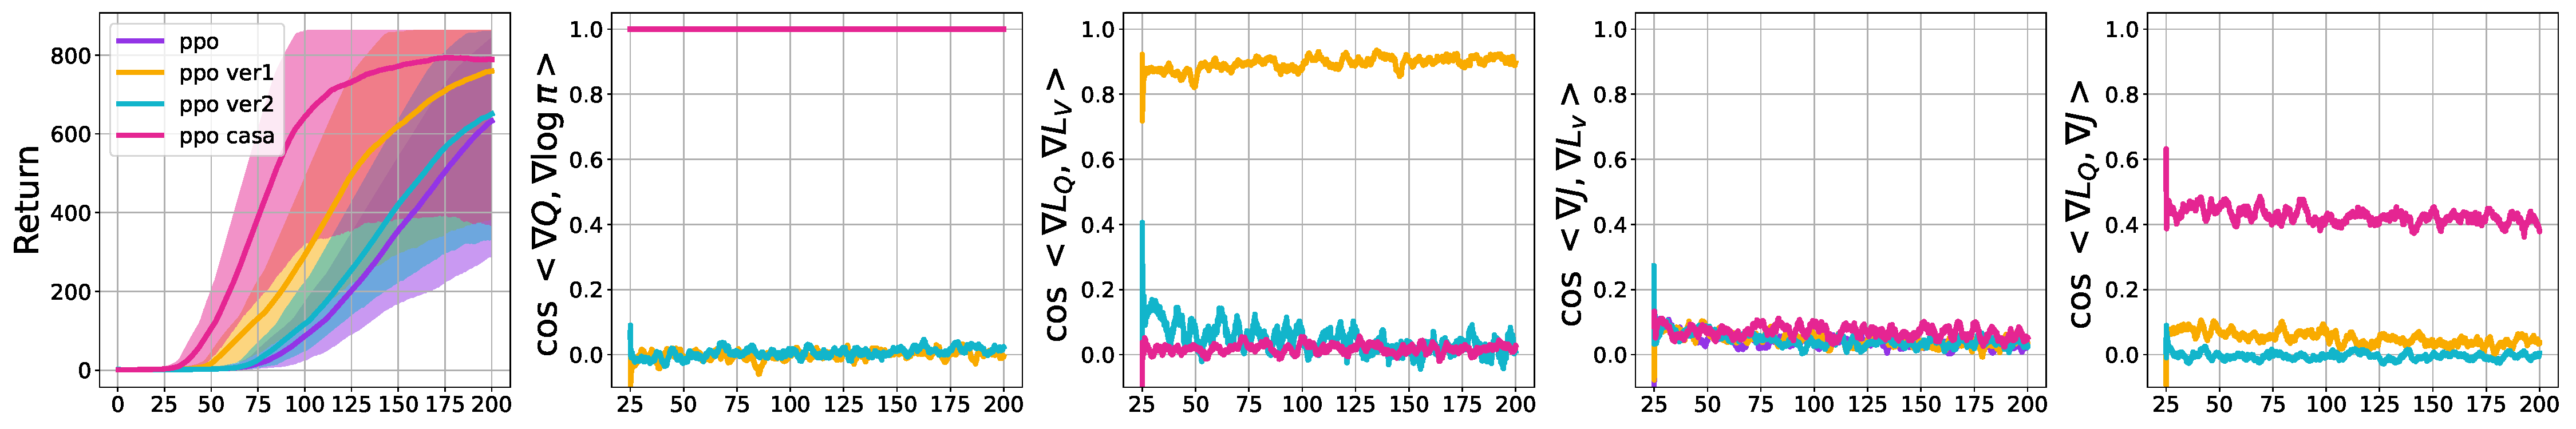
\includegraphics[width=\linewidth]{body/app_fig/app_ppo_Breakout.pdf}

% 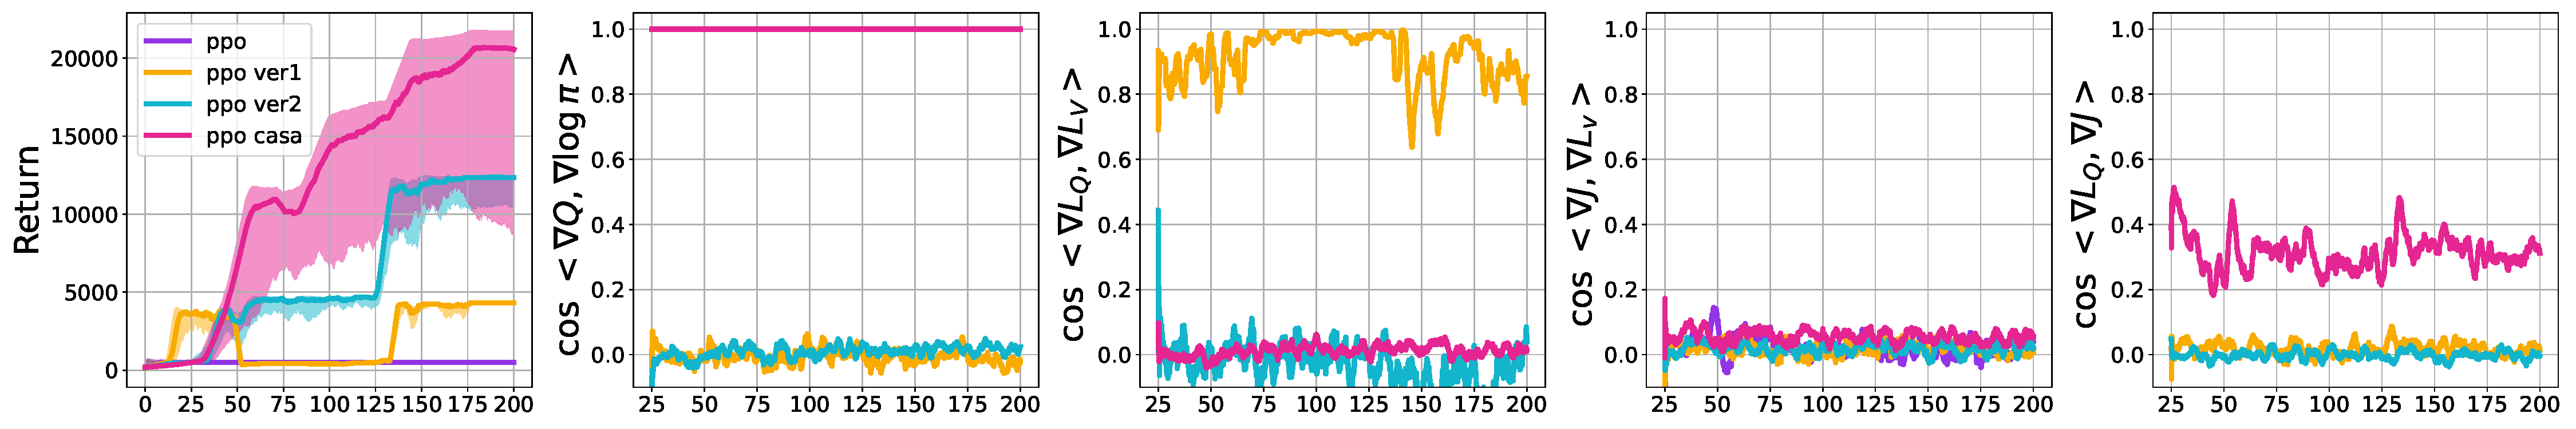
\includegraphics[width=\linewidth]{body/app_fig/app_ppo_Qbert.pdf}

% 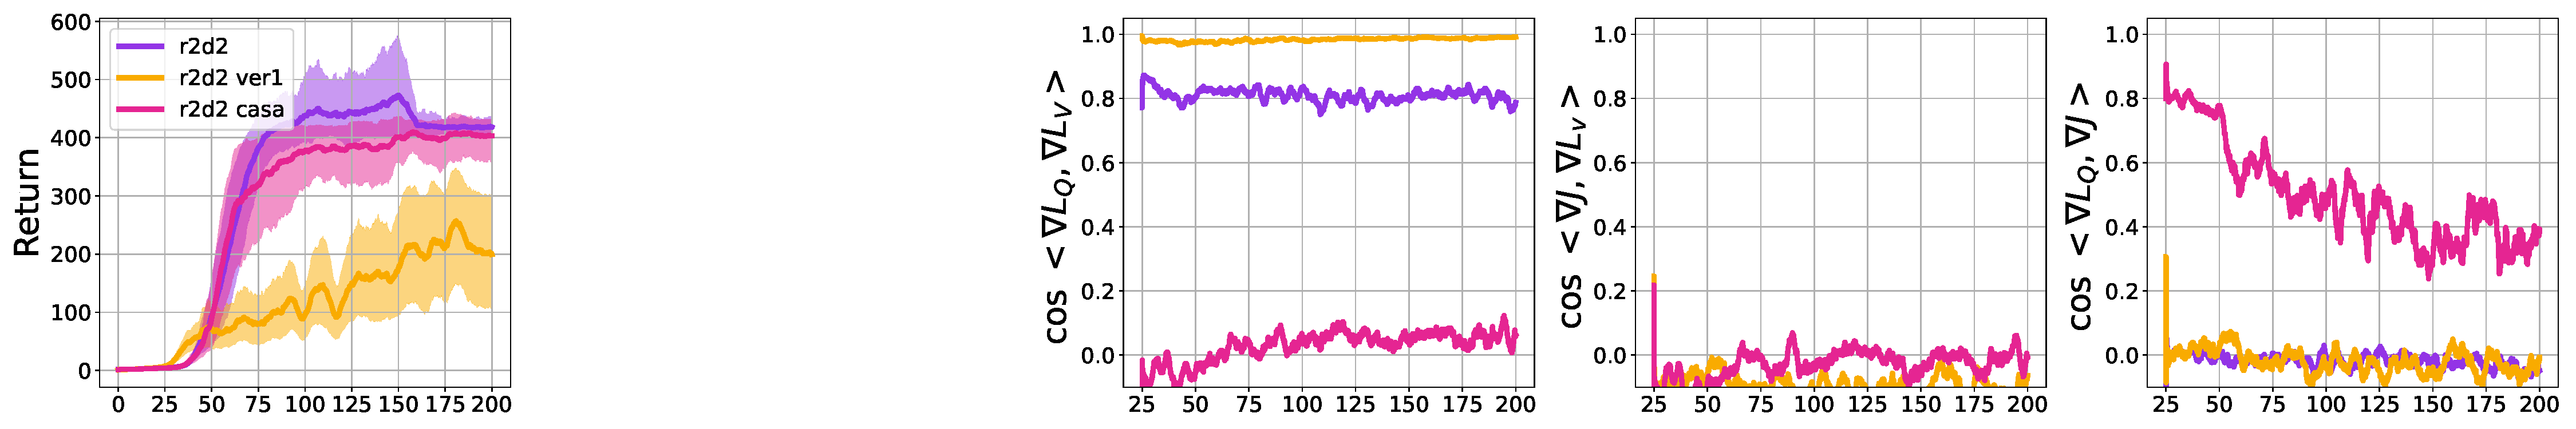
\includegraphics[width=\linewidth]{body/app_fig/app_r2d2_Breakout.pdf}


% 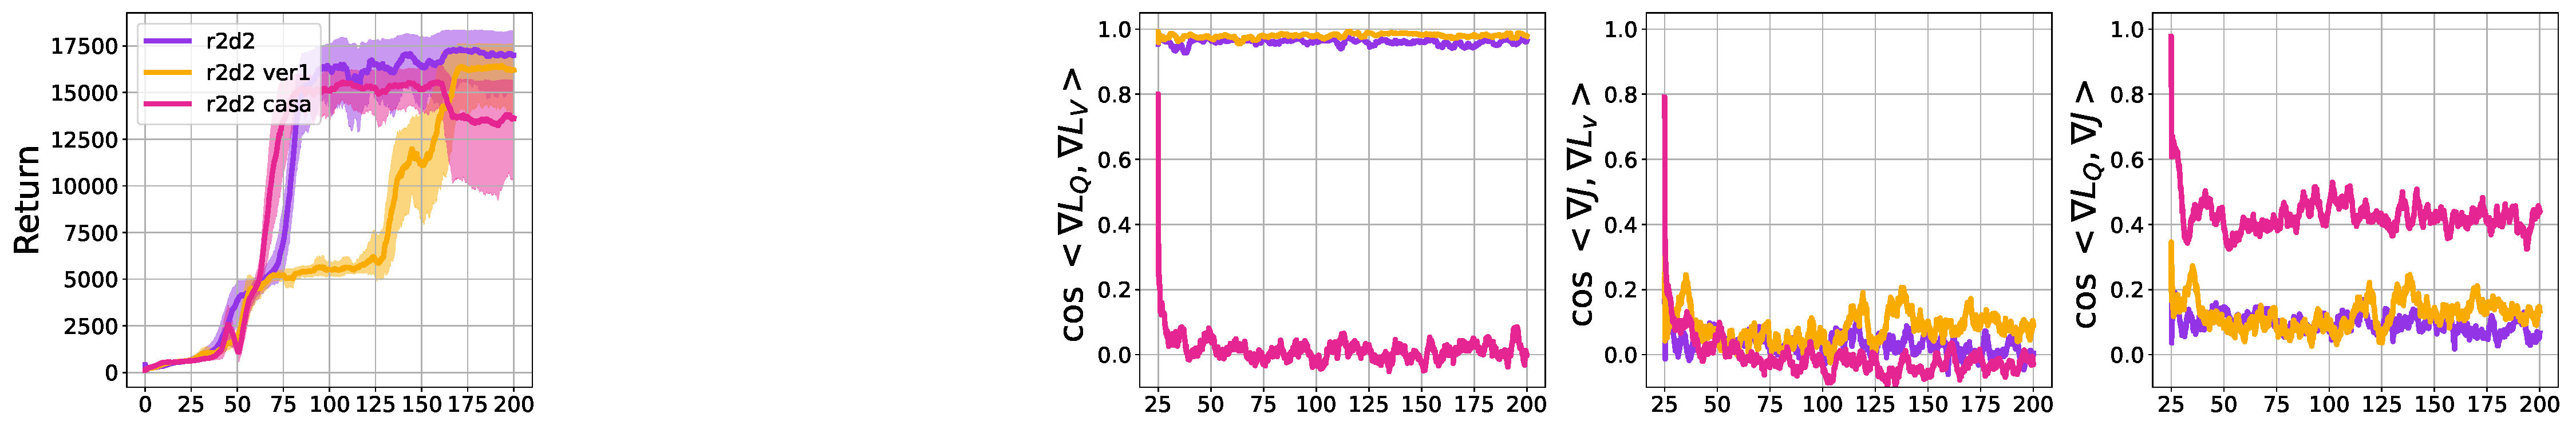
\includegraphics[width=\linewidth]{body/app_fig/app_r2d2_Qbert.pdf}
% \caption{Angles of Gradients and Returns of versions of PPO and R2D2 defined in Table \ref{tab:ppo_mtv} and Table \ref{tab:r2d2_mtv}.}
% \label{fig:mtv_app}
% \end{figure}

% \clearpage

% \changnan{casa summary deleted}
% \section{CASA summary}
% \begin{figure}[ht]
% \centering
% 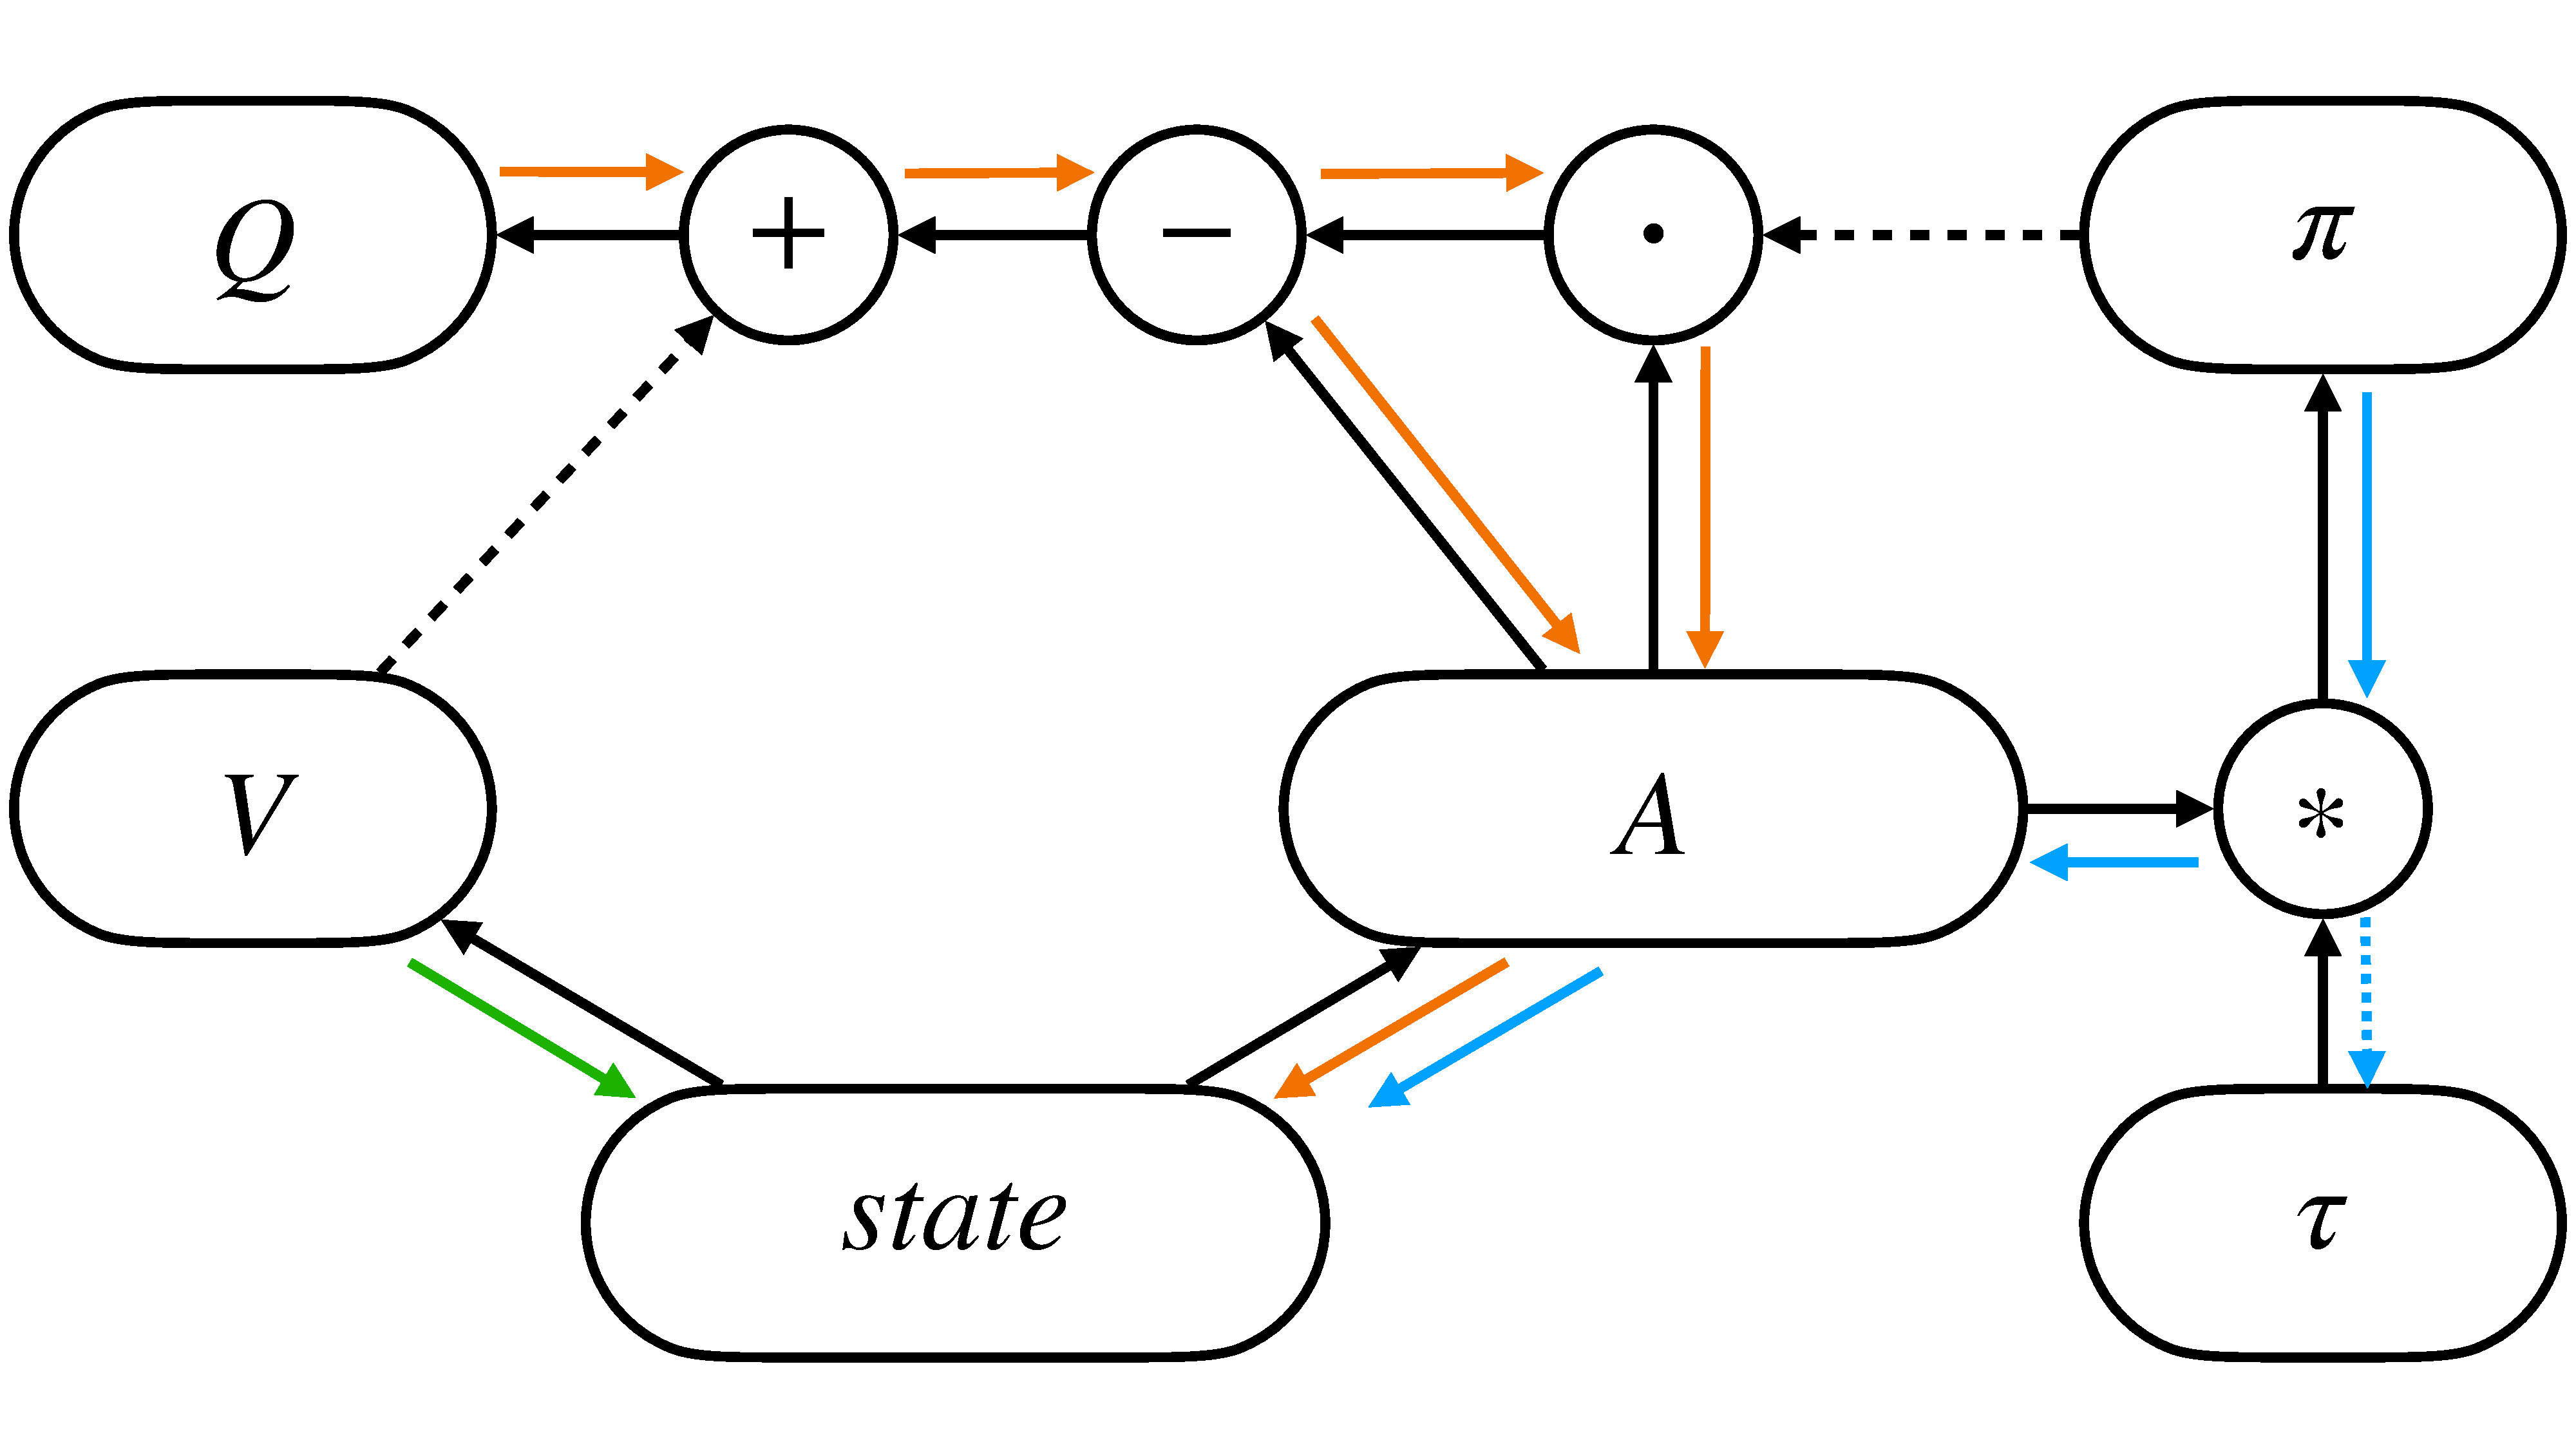
\includegraphics[width=0.4\textwidth,bb= 0 0 1800 1100]{body/figures/CASA.pdf}
% \caption{
% \textbf{Black} lines represent the forward process.
% \textbf{Dotted} black lines represent the \textit{stop gradient} operator in the forward process. 
% \textbf{Colorful} lines represent backpropagation from different loss functions. 
% Specifically, \textbf{blue} lines represent $\mathbb{E}_\pi [(Q^\pi-V)\nabla \log \pi]$, 
% \textbf{orange} lines represent $\mathbb{E}_\pi [(Q^\pi-Q)\nabla Q]$,
% and \textbf{green} lines represent $\mathbb{E}_\pi [(Q^\pi-V)\nabla V]$.}
% \label{fig:casa}
% \end{figure}
% \section{motivation experiments}

\clearpage

{\colorred \section{On Discussing Application of CASA on Continuous Action Space}
\label{app:cts_space}

As we can see CASA is only applied to discrete action space in the main context, we make a discussion on whether CASA is applicable on continuous action space. 
For brevity, we let $\tau=1$ and write \eqref{eq:casa} as:
\begin{equation}
\left\{
    \begin{aligned}
        &\pi = \text{softmax}(A), \\
        &\Bar{A} = A - \mathbb{E}_{\pi} [A], \\
        &Q = \Bar{A} + sg(V).
    \end{aligned}
\right. 
\end{equation}
The difficulty comes from estimating two quantities, one is $\text{softmax}(A)$, the other is $\mathbb{E}_{\pi} [A]$. 
This comes from the fact that discrete action space is countable so these two quantities are expressed in a closed-form, while continuous action space is uncountable so an accurate estimation of these two quantities is intractable. 
We can surely apply Monte Carlo methods to approximate, but a more elegant close-form expression may be preferred. 
Then this becomes another problem: \textit{how to estimate (state-action values / advantages / policy probabilities) of all actions in a continuous action space efficiently without loss of generality?}
This is another representational design problem, which is out of scope of this paper, so we don't touch much about it. 
But with the hope of inspiring a better solution to this problem, we provide one practical way of applying CASA on continuous action space based on kernel-based machine learning. 

Let $a_0, \dots, a_k$ to be basis actions in the action space. 
Let $A(s, a_0), \dots, A(s, a_k)$ to be advantage functions for tuples of states and basis actions. 
They can either share parameters or be isolated. 
Let $K(\cdot, \cdot)$ be a kernel function defined on the product of two action spaces. 
For any $a$ in the action space, we can estimate $A(s, a)$ by a decomposition such like $$A(s, a) = \frac{1}{Z_a} (K(a_0, a) A(s, a_0) + \dots + K(a_k, a) A(s, a_k)),$$ where $Z_a = \sum_{i=0}^k K(a_i, a)$ is a normalization constant. 

Since $K(\cdot, a)$ is a closed-form function of $a$, and $|\{A(s, a_0), \dots, A(s, a_k)\}|$ is finite, we can make a closed-form expression of both $\text{softmax}(A)$ and $\mathbb{E}_{\pi} [A]$. 
Then we can apply CASA directly on this expression, with one function estimates $V$ and the other function estimates advantages of all actions in a closed-form with only state as input.  
The policy is defined directly by $\text{softmax}$ of all advantages. 
In details, we define
\begin{equation}
\left\{
    \begin{aligned}
        &\pi(s, a) = \exp (A(s, a)) / \int_{a} \exp (A(s, a)) da, \\
        &\Bar{A}(s, a) = A(s, a) - \int_{a} sg(\pi(s, a)) A(s, a) da, \\
        &Q(s, a) = \Bar{A}(s, a) + sg(V(s)).
    \end{aligned}
\right. 
\end{equation}

Then it satisfies the consistency of CASA on continuous action space.
$$
\begin{aligned}
    \nabla \log \pi(s, a) &= \nabla A(s, a) - \frac{\nabla \int_{a} \exp (A(s, a)) da}{\int_{a} \exp (A(s, a)) da} \\
    &= \nabla A(s, a) - \frac{ \int_{a} \exp (A(s, a)) \nabla A(s, a) da}{\int_{a} \exp (A(s, a)) da} \\
    &= \nabla A(s, a) - \int_{a} \frac{  \exp (A(s, a)) }{\int_{a} \exp (A(s, a)) da} \nabla A(s, a) da \\
    &= \nabla A(s, a) - \int_{a} \pi(s, a) \nabla A(s, a) da \\
    &= \nabla \Bar{A}(s, a) = \nabla Q(s, a). 
\end{aligned}
$$
}

\section{DR-Trace}
\label{app:drtrace}

% One simple choice is to learn $V$ and $\pi$ by V-Trace \citep{impala} and to learn $Q$ by ReTrace \citep{retrace}. 
% \citep{impala} shows that $V^{\Tilde{\pi}}$ estimated by V-Trace converges to $V^*$ that corresponds to some $\Tilde{\pi}_{VTrace}$.
% Respectively, \citep{retrace} shows that $Q^{\Tilde{\pi}}$ estimated by ReTrace converges to $Q^*$ that corresponds to some $\Tilde{\pi}_{ReTrace}$.

As CASA estimates $(V, Q, \pi)$, we would ask
\textbf{i)} how to guarantee that $\Tilde{\pi}_{VTrace} = \Tilde{\pi}_{ReTrace}$, 
\textbf{ii)} how to exploit $(V, Q, \pi)$ to make a better estimation. 
Though we can apply V-Trace to estimate $V$ and ReTrace to estimate $Q$ with proper hyperparameters to guarantee $\Tilde{\pi}_{VTrace} = \Tilde{\pi}_{ReTrace}$, it's more reasonable to estimate $(V, Q)$ together. 
Inspired by Doubly Robust, which is shown to maximally reduce the variance, we introduce DR-Trace, which estimates $V$ by 
$$
\label{eq:dr-v}
    \begin{aligned}
        V_{DR}^{\Tilde{\pi}} (s_t) &\overset{def}{=} \mathbb{E}_{\mu} [ 
        V(s_t) + \sum_{k \geq 0} \gamma^k 
     c_{[t:t+k-1]} \rho_{t+k}  \delta^{DR}_{t+k} ],  
    \end{aligned}
$$
{\colorred where $\mu$ is the behavior policy}, $\delta^{DR}_t \overset{def}{=} r_t + \gamma V(s_{t+1}) - Q(s_t, a_t)$ is one-step Doubly Robust error, $\rho_t \overset{def}{=} \min\{\frac{\pi_t}{\mu_t}, \Bar{\rho} \}$ and $c_t \overset{def}{=} \min\{\frac{\pi_t}{\mu_t}, \Bar{c}\}$ are clipped per-step importance sampling, $c_{[t: t+k]} \overset{def}{=} \prod_{i=0}^{k} c_{t+i}$.

With one step Bellman equation, we estimate $Q$ by
$$
\label{eq:dr-q}
    \begin{aligned}
         Q_{DR}^{\Tilde{\pi}} (s_t, a_t) 
         &\overset{def}{=} \mathbb{E}_{s_{t+1}, r_t \sim p(\cdot, \cdot | s_t, a_t)} [  r_t + \gamma   V_{DR}^{\Tilde{\pi}} (s_{t+1}) ] 
        \\
        %  &=  \mathbb{E}_{\mu} [ r_t + \gamma V(s_{t + 1}) +
        % \gamma \sum_{k \geq 0} \gamma^k 
        % c_{[t+1:t+k]} \rho_{t+1+k}
        % \delta^{DR}_{t+1+k} V
        % ]
        % \\
        %  &= \mathbb{E}_{\mu}   [
        % Q(s_t, a_t) + \delta_t^{DR}V + \sum_{k \geq 1}  \gamma^k
        % c_{[t+1:t+k-1]} \rho_{t+k}
        % \delta^{DR}_{t+k} V
        % ],
        % \\
        &=  \mathbb{E}_{\mu}   [
        Q(s_t, a_t) + \sum_{k \geq 0}  \gamma^k
        c_{[t+1:t+k-1]} \Tilde{\rho}_{t, k}
        \delta^{DR}_{t+k}
        ], 
    \end{aligned}
$$
where $\Tilde{\rho}_{t, k} =  1_{\{k=0\}} + 1_{\{k > 0\}} \rho_{t+k}$.

% Compared to \eqref{eq:dr-v}, $c_{[t+1:t+k-1]} \Tilde{\rho}_{t, k}$ in \eqref{eq:dr-q} doesn't multiply importance sampling ratio of $a_t$, which meets the same intuition as \eqref{eq:vtrace} and \eqref{eq:retrace}.\\
\begin{theorem}
    Define $\Bar{A} = A - \mathbb{E}_\pi[A]$, $Q = \Bar{A} + sg(V)$,
    $$
    \begin{aligned}
    &\mathscr{T}(Q) \overset{def}{=} \mathbb{E}_{\mu}   [
        Q(s_t, a_t) + \sum_{k \geq 0}  \gamma^k
        c_{[t+1:t+k-1]} \Tilde{\rho}_{t, k}
        \delta^{DR}_{t+k}
        ], \\
    &\mathscr{S}(V) \overset{def}{=} \mathbb{E}_{\mu}   [
        V(s_t) + \sum_{k \geq 0}  \gamma^k
        c_{[t:t+k-1]} \rho_{t, k}
        \delta^{DR}_{t+k}
        ], \\
    &\mathscr{U}(Q, V) = (\mathscr{T}(Q) - \mathbb{E}_\pi[Q] + \mathscr{S}(V), \mathscr{S}(V)), \\
    &\mathscr{U}^{(n)}(Q, V) = \mathscr{U}(\mathscr{U}^{(n-1)}(Q, V)),
    \end{aligned}
    $$
    then $\mathscr{U}^{(n)}(Q, V) \rightarrow (Q^{\Tilde{\pi}}, V^{\Tilde{\pi}})$ that corresponds to 
    $$
        \Tilde{\pi}(a|s) = \frac
        {\min \left\{\Bar{\rho} \mu (a|s), \pi(a|s)\right\}}
        {\sum_{b \in \mathcal{A}}\min \left\{\Bar{\rho} \mu (b|s), \pi(b|s)\right\}}.
    $$ as $n \rightarrow +\infty$.
\label{thm:dr}
\end{theorem}
\begin{proof}
    See Appendix \ref{app:proof}, Theorem \ref{thm_app:dr}.
\end{proof}
Theorem \ref{thm:dr} shows that DR-Trace is a contraction mapping and $(V, Q)$ converges to $(V^{\Tilde{\pi}}, Q^{\Tilde{\pi}})$ that corresponds to 
$$
    \begin{aligned}
        \Tilde{\pi}(a|s) = \frac
        {\min \left\{\Bar{\rho} \mu (a|s), \pi(a|s)\right\}}
        {\sum_{b \in \mathcal{A}}\min \left\{\Bar{\rho} \mu (b|s), \pi(b|s)\right\}}.
    \end{aligned}
$$

% At training time, the policy evaluation is achieved by updating $\theta$ to minimize $l2$ losses
% $$
% \begin{aligned}
%     L_V(\theta) &= \mathbb{E}_\pi [ (V_\theta(s_t) -  V_{DR}^{\Tilde{\pi}} (s_t))^2 ], \\
%     L_Q(\theta) &= \mathbb{E}_\pi [ (Q_\theta(s_t, a_t) -  Q_{DR}^{\Tilde{\pi}} (s_t, a_t))^2 ],
% \end{aligned}
% $$ 
% which gives the ascent direction of $\theta$ by
% \begin{equation}
% \label{eq:grad_qv}
%     \begin{aligned}
%         \nabla_\theta L_V(\theta)
%         &= \mathbb{E}_\pi \left[ (V_{DR}^{\Tilde{\pi}} (s_t) - V_\theta(s_t) ) \nabla V_\theta(s_t) \right], \\
%         \nabla_\theta L_Q(\theta)
%         &= \mathbb{E}_\pi \left[ (Q_{DR}^{\Tilde{\pi}} (s_t, a_t) - Q_\theta(s_t, a_t)) \nabla Q_\theta(s_t, a_t) \right].
%     \end{aligned}
% \end{equation}
% And we make the policy improvement by policy gradient, which gives the ascent direction of $\theta$ by 
% \begin{equation}
% \label{eq:grad_pi}
% \begin{aligned}
%     \nabla_\theta \mathcal{J}(\tau, \theta) = \mathbb{E}_\mu \left[\tau \rho_t (Q_{DR}^{\Tilde{\pi}} (s_t, a_t) - V_\theta(s_t) ) \nabla_\theta \log \pi_t \right],
% \end{aligned}
% \end{equation}
% where $\mathcal{J} (\tau, \theta) = \tau \mathbb{E}_\pi [\sum \gamma^t r_t]$.
% It takes an additional $\tau$, which frees the scale of gradient from $\tau$.

% Finally, the gradient ascent direction of $\theta$ is given by
% \begin{equation}
%     \label{eq:grad_all}
%     \alpha_1 \nabla_\theta L_V + \alpha_2 \nabla_\theta L_Q + \alpha_3 \nabla_\theta \mathcal{J}.
% \end{equation}

% \textbf{Full algorithm is described in Appendix \ref{app:casa}.}
% Note that \eqref{eq:grad_all} doesn't need any entropy regularization. 
% We will discuss why this happens in section \ref{sec:equiv} and how CASA controls the exploration in section \ref{sec:ent_control}.


\begin{figure}[h]
    \centering
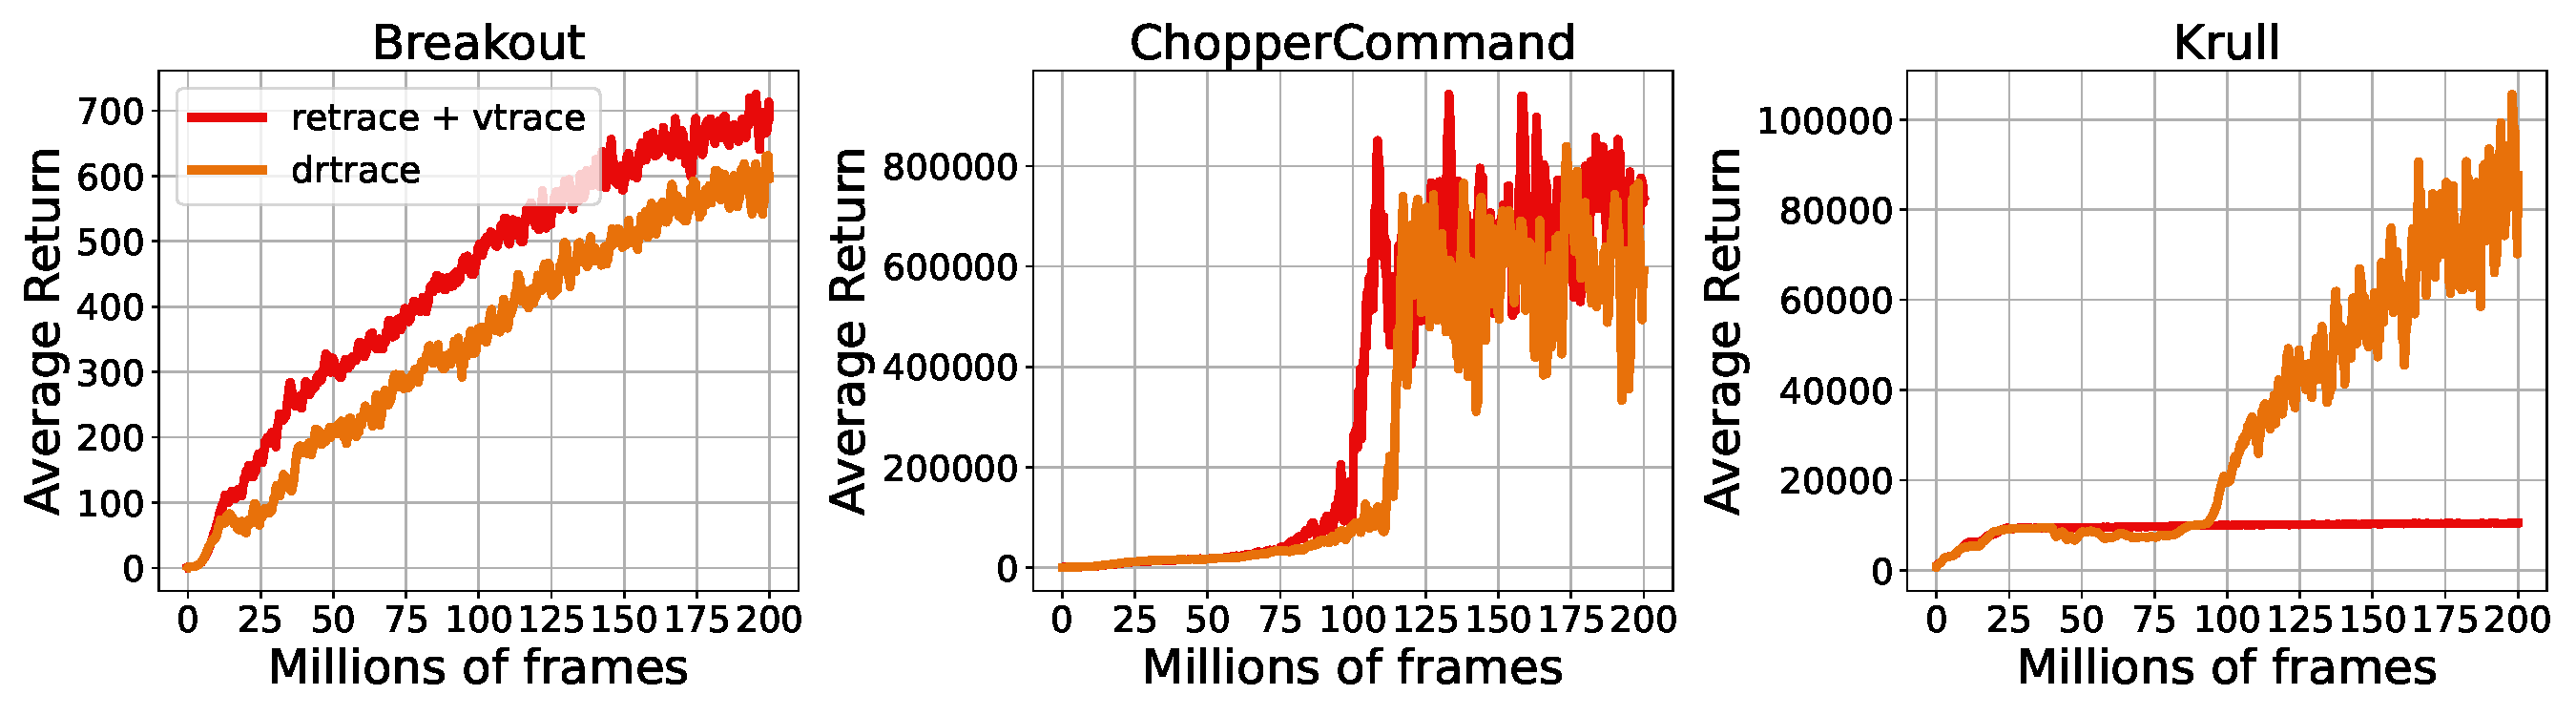
\includegraphics[width=\linewidth]{body/ablation/dr_ablation.pdf}
    \caption{Ablation study for w/wo DR-Trace on Breakout, ChopperCommand and Krull.}
    \label{fig:app_dr_trace}
\end{figure}

According to our proof, DR-Trace should work similar to V-Trace and ReTrace, as the convergence rate and the limitation are same. 
We compare DR-Trace with V-Trace+ReTrace in Figure \ref{fig:app_dr_trace}, where we replace estimation of state values by V-Trace and estimation of state-action values by ReTrace. 
We call V-Trace+ReTrace as No-DR-Trace for brevity. 
No-DR-Trace performs better on Breakout and ChopperCommand, but fails to make a breakthrough on Krull. 
Recalling the fact that Doubly Robust can maximally reduce the variance of Bellman error, No-DR-Trace is less stable but also potential to achieve a better performance. 
A conclusion cannot be made about No-DR-Trace, as this phenomenon means that No-DR-Trace is less stable than DR-Trace, but it also holds the potential to achieve a better performance.

% \clearpage


\section{Proofs}
\label{app:proof}

\theoremstyle{plain}
% \setcounter{Lemma}{0}
\newtheorem{Lemma_app}{Lemma}[section]
\newtheorem{Theorem_app}{Theorem}[section]
\theoremstyle{definition}
\newtheorem*{Remark_app}{Remark}
\theoremstyle{remark}

% \begin{Lemma_app}
% Let 
% $g \in \textbf{C}^{1}(\mathbb{R}^{n}): \mathbb{R}^{n} \to \mathbb{R}^{n}, \ f \in \textbf{C}^{1}(\mathbb{R}^{n+k}): \mathbb{R}^{n+k} \to \mathbb{R}^{n}.
% $\\
% If
% $
% \nabla_x g(x) = \nabla_x f(x, y)$, for $\forall x\in \mathbb{R}^{n}, y\in \mathbb{R}^k,
% $
% then $\exists$ $c \in \textbf{C}^{1}(\mathbb{R}^{k}): \mathbb{R}^{k} \to \mathbb{R}^{n}$, s.t. $f(x, y) = g(x) + c(y)$.
% \label{lemma_app:func_sep}
% \end{Lemma_app}
% \begin{proof}

% Let $\Tilde{f}(x, y) = f(x, y) - g(x)$.

% Since $\nabla_x g(x) = \nabla_x f(x, y)$, we have 
% $$
% \nabla_x \Tilde{f} = 0, \ for \ \forall x\in \mathbb{R}^{n}, y\in \mathbb{R}^k.
% $$

% So $\Tilde{f}$ is a constant function w.r.t $x$, which can be denoted as $c(y) = \Tilde{f}(x, y)$.

% Hence, $f(x, y) = g(x) + c(y)$.
% \end{proof}

\begin{Lemma_app}
(i) Define $\pi = softmax(A / \tau)$, then $\nabla \log \pi = (\textbf{1} - \pi) \frac{\nabla A}{\tau}$. 
(ii) Denote $sg$ to be stop gradient and define $\Bar{A} = A - \mathbb{E}_\pi [A]$, $Q = \Bar{A} + sg(V)$, then $\nabla Q = (\textbf{1} - \pi) \nabla A$.
\label{lemma_app:vannila_grad}
\end{Lemma_app}
\begin{proof}

As $Q = \Bar{A} + sg(V) = A - sg(\pi)\cdot A + sg(V)$, it's obvious that $\nabla Q = (\textbf{1} - \pi) \nabla A$.

For $\log \pi$, it's a standard derivative of cross entropy, so we have $\nabla \log \pi = (\textbf{1} - \pi) \nabla (A / \tau) = (\textbf{1} - \pi) \frac{\nabla A}{\tau}$.
\end{proof}

\begin{Lemma_app}
Define $\Bar{A}= A - \mathbb{E}_\pi[A]$, $Q = \Bar{A} + sg(V), \pi = softmax(A / \tau)$, then 
$$
\mathbb{E}_\pi \left[ (Q - V) \nabla \log \pi \right]
= - \tau \nabla \textbf{H}[\pi].
$$
\label{lemma_app:eqiv_pg_ent}
\end{Lemma_app}
\begin{proof}
Since 
$$
\pi = \exp(A / \tau) / Z,\ Z = \int_\mathcal{A} \exp(A / \tau),
$$
we have 
$$
A = \tau \log \pi + \tau \log Z.
$$
Based on the observation that $\mathbb{E}_\pi \left[ f(s) \nabla \log \pi (\cdot | s) \right] = 0$, 
we have 
$$\mathbb{E}_\pi \left[ \mathbb{E}_\pi[A] \cdot \nabla \log \pi \right] = 0,$$ 
$$\mathbb{E}_\pi \left[ \log Z \cdot \nabla \log \pi \right] = 0.$$

On the one hand,
$$
\begin{aligned}
    \mathbb{E}_\pi \left[ (Q - V) \nabla \log \pi \right]
    &= \mathbb{E}_\pi \left[ A \nabla \log \pi \right] 
    - \mathbb{E}_\pi \left[ \mathbb{E}_\pi[A] \cdot \nabla \log \pi \right] \\
    &= \tau \mathbb{E}_\pi \left[ \log \pi \nabla \log \pi \right]
    + \tau \mathbb{E}_\pi \left[ \log Z \cdot \nabla \log \pi \right] \\
    &= \tau \mathbb{E}_\pi \left[ \log \pi \nabla \log \pi \right].
\end{aligned}
$$

On the other hand, 
$$
\begin{aligned}
    \nabla \textbf{H} [\pi] 
    &= - \nabla \int_\mathcal{A} \pi_i \log \pi_i \\
    &= - \int_\mathcal{A}  \nabla \pi_i \cdot \log \pi_i - \int_\mathcal{A} \pi_i \nabla \log \pi_i  \\
    &= - \int_\mathcal{A}  \pi_i \nabla \log \pi_i \cdot \log \pi_i - \int_\mathcal{A}  \pi_i \frac{\nabla \pi_i}{\pi_i} \\
    &= - \mathbb{E}_\pi \left[ \log \pi \nabla \log \pi \right].
\end{aligned}
$$
Hence, $
\mathbb{E}_\pi \left[ (Q - V) \nabla \log \pi \right]
= - \tau \nabla \textbf{H}[\pi]
$.
\end{proof}

\begin{Theorem_app}
    Define $\Bar{A} = A - \mathbb{E}_\pi[A]$, $Q = \Bar{A} + sg(V)$.
    Define $$
    \begin{aligned}
    &\mathscr{T}(Q) \overset{def}{=} \mathbb{E}_{\mu}   [
        Q(s_t, a_t) + \sum_{k \geq 0}  \gamma^k
        c_{[t+1:t+k-1]} \Tilde{\rho}_{t, k}
        \delta^{DR}_{t+k}
        ], \\
    &\mathscr{S}(V) \overset{def}{=} \mathbb{E}_{\mu}   [
        V(s_t) + \sum_{k \geq 0}  \gamma^k
        c_{[t:t+k-1]} \rho_{t, k}
        \delta^{DR}_{t+k}
        ], \\
    &\mathscr{U}(Q, V) = (\mathscr{T}(Q) - \mathbb{E}_\pi[Q] + \mathscr{S}(V), \mathscr{S}(V)), \\
    &\mathscr{U}^{(n)}(Q, V) = \mathscr{U}(\mathscr{U}^{(n-1)}(Q, V)),
    \end{aligned}
    $$
    then $\mathscr{U}^{(n)}(Q, V) \rightarrow (Q^{\Tilde{\pi}}, V^{\Tilde{\pi}})$ that corresponds to 
    $$
        \Tilde{\pi}(a|s) = \frac
        {\min \left\{\Bar{\rho} \mu (a|s), \pi(a|s)\right\}}
        {\sum_{b \in \mathcal{A}}\min \left\{\Bar{\rho} \mu (b|s), \pi(b|s)\right\}}.
    $$ as $n \rightarrow +\infty$.
\label{thm_app:dr}
\end{Theorem_app}
\begin{Remark_app}
$\mathscr{T}(Q) - \mathbb{E}_\pi[Q] + \mathscr{S}(V)$ is \textbf{exactly} how $Q$ is updated at training time. 
Since $Q = \Bar{A} + sg(V)$, if we apply gradient ascent on $Q$ and $V$ in directions $\nabla L_Q(\theta)$ and $\nabla L_V(\theta)$ respectively, change of $Q$ comes from two aspects. One comes from $\nabla L_Q(\theta)$, which changes $A$, the other comes from $\nabla L_V(\theta)$, which changes $V$. Because the gradient of $V$ is stopped when estimating $Q$, the latter is captured by "minus old baseline, add new baseline", which is $- \mathbb{E}_\pi[Q] + \mathscr{S}(V)$ in Theorem \ref{thm_app:dr}.
\end{Remark_app}
\begin{proof}
 Define
 $$
 \begin{aligned}
        \widetilde{\mathscr{T}}(Q) &= - \mathbb{E}_\pi[Q] + \mathscr{T}(Q), \\
        \widetilde{\mathscr{U}}(Q, V) &= (\widetilde{\mathscr{T}}(Q), \mathscr{S}(V)), \\
        \widetilde{\mathscr{U}}^{(n)}(Q, V) &=   \widetilde{\mathscr{U}}(\widetilde{\mathscr{U}}^{(n-1)}(Q, V)).
 \end{aligned}
 $$
By Lemma \ref{lemma_app:dr_q}, $\widetilde{\mathscr{T}}^{(n)}(Q)$ converges to some $A^*$ as $n \rightarrow \infty$. This process will not influence the estimation of $V$ as the gradient of $V$ is stopped when estimating $Q$. According to the proof, $A^*$ does not depend on $V$. \\
By Lemma \ref{lemma_app:dr_v}, $\mathscr{S}^{(n)}(V)$ converges to some $V^*$ as $n \rightarrow \infty$. \\
Hence, we have
$$
\widetilde{\mathscr{U}}^{(n)}(Q, V) \rightarrow (A^*, V^*)\ \ as\ \ n \rightarrow +\infty. 
$$
By definition, 
$$
\mathscr{U}(Q, V) = (\widetilde{\mathscr{T}}(Q) + \mathscr{S}(V), \mathscr{S}(V)),
$$
we can regard $\widetilde{\mathscr{T}}(Q) + \mathscr{S}(V)$ as $Q$ and regard $\mathscr{S}(V)$ as $V$, then
$$
\begin{aligned}
    \mathscr{U}^{(2)}(Q, V) 
    &= \mathscr{U}(\widetilde{\mathscr{T}}(Q) + \mathscr{S}(V), \mathscr{S}(V)) \\
    &= (\mathscr{T}(\widetilde{\mathscr{T}}(Q) + \mathscr{S}(V)) -\mathscr{S}(V) + \mathscr{S}^{(2)}(V), \mathscr{S}^{(2)}(V)) \\
    &= (\widetilde{\mathscr{T}}^{(2)}(Q) + \mathscr{S}^{(2)}(V), \mathscr{S}^{(2)}(V)).
\end{aligned}
$$
By induction, 
$$
\begin{aligned}
    \mathscr{U}^{(n)}(Q, V) &= (\widetilde{\mathscr{T}}^{(n)}(Q) + \mathscr{S}^{(n)}(V), \mathscr{S}^{(n)}(V)) \\
    &\rightarrow (A^*+V^*, V^*)\ \ as\ \ n\rightarrow + \infty.
\end{aligned}
$$
Same as \citep{impala}, 
$$
    \Tilde{\pi}(a|s) = \frac
    {\min \left\{\Bar{\rho} \mu (a|s), \pi(a|s)\right\}}
    {\sum_{b \in \mathcal{A}}\min \left\{\Bar{\rho} \mu (b|s), \pi(b|s)\right\}}.
$$ 
is the policy s.t. the Bellman equation holds, which is 
$$\mathbb{E}_\mu[\rho_t (r_t + \gamma V_{t+1} - V_t) | \mathscr{F}_t] = 0,$$ and $\mathscr{U}(Q^{\Tilde{\pi}}, V^{\Tilde{\pi}}) = (Q^{\Tilde{\pi}}, V^{\Tilde{\pi}})$. \\
So we have
$(A^*+V^*, V^*) = (Q^{\Tilde{\pi}}, V^{\Tilde{\pi}}).$
\end{proof}

\begin{Lemma_app}
Define $\Bar{A}= A - \mathbb{E}_\pi[A]$, $Q = \Bar{A} + sg(V)$,
then operator 
$$
    \mathscr{T}(Q) \overset{def}{=} \mathbb{E}_{\mu}   [
        Q(s_t, a_t) + \sum_{k \geq 0}  \gamma^k
        c_{[t+1:t+k-1]} \Tilde{\rho}_{t, k}
        \delta^{DR}_{t+k}
        ]
$$
is a contraction mapping w.r.t. $Q$.
\label{lemma_app:dr_q}
\end{Lemma_app}
\begin{Remark_app}
Note that $\mathscr{T}(Q)$ is exactly \eqref{eq:dr-q}. 

Since $Q = A + sg(V)$, the gradient of $V$ is stopped when estimating $Q$, updating $Q$ will not change $V$, which is equivalent to updating $A$.
Without loss of generality, we assume $V$ is fixed as $V^*$ in the proof.
\end{Remark_app}
\begin{proof}

$\Bar{A} = A - \mathbb{E}_\pi[A]$ shows $\mathbb{E}_\pi[\Bar{A}] = 0$, which guarantees that no matter how we update $A$, we always have $\mathbb{E}_\pi[Q] = V^*$.

Based on above observations, define 
$$
    \widetilde{\mathscr{T}}(Q) \overset{def}{=} - \mathbb{E}_\pi [Q] + \mathscr{T}(Q).
$$

It's obvious that we only need to prove $\widetilde{\mathscr{T}}(Q)$ is a contraction mapping.

For brevity, we denote $$Q_t = Q(s_t, a_t), A_t = A(s_t, a_t), V^*_t = V^*(s_t).$$

Noticing that $\Tilde{\rho}_{t, 0} = 1$, let $\mathscr{F}$ represent filtration, we can rewrite $\widetilde{\mathscr{T}}$ as 
\begin{equation}
\label{eq:dr_a_2}
\begin{aligned}
    \widetilde{\mathscr{T}}(Q)
    &= \mathbb{E}_{\mu}   [
        A_t + \sum_{k \geq 0}  \gamma^k
        c_{[t+1:t+k-1]} \Tilde{\rho}_{t, k}
        \delta^{DR}_{t+k}
        ] \\
    &= \mathbb{E}_{\mu}   [
        -V^*_t + \sum_{k \geq 0}  \gamma^k
        c_{[t+1:t+k-1]} \Tilde{\rho}_{t, k}
        r_{t+k}
        + 
        \sum_{k \geq 0}  \gamma^{k+1}
        c_{[t+1:t+k-1]} \Delta_k ],
        \\
\end{aligned}
\end{equation}
where 
\begin{equation}
\label{eq:dr_delta}
    \Delta_k = \mathbb{E}_{\mu}\left[\Tilde{\rho}_{t, k} V^*_{t+k+1} - c_{t+k} \Tilde{\rho}_{t, k+1} Q_{t+k+1} | \mathscr{F}_{t+k}\right].
\end{equation}
By definition of $Q$,
$$
    \mathbb{E}_{\mu}[V_{t+k+1}^*|\mathscr{F}_{t+k}] 
    = \mathbb{E}_{\mu}[
    \mathbb{E}_\pi[Q_{t+k+1}|\mathscr{F}_{t+k+1}]
    |\mathscr{F}_{t+k}], \\
    % \geq&  \mathbb{E}_{\mu}[
    % \mathbb{E}_\mu[\Tilde{\rho}_{t, k+1} Q_{t+k+1}|\mathscr{F}_{t+k+1}]
    % |\mathscr{F}_{t+k}], 
$$
we can rewrite \eqref{eq:dr_delta} as
\begin{equation}
\label{eq:dr_q_delta}
\Delta_k = \mathbb{E}_{\mu}[
(
\Tilde{\rho}_{t, k} \frac{\pi_{t+k+1}}{\mu_{t+k+1}}- c_{t+k} \Tilde{\rho}_{t, k+1} 
) Q_{t+k+1} | \mathscr{F}_{t+k}
].
\end{equation}
For any $Q_1 = A_1 + sg(V^*)$, $Q_2 = A_2 + sg(V^*)$, since
$$
\mathbb{E}_{\mu}[
(
\Tilde{\rho}_{t, k} \frac{\pi_{t+k+1}}{\mu_{t+k+1}}- c_{t+k} \Tilde{\rho}_{t, k+1} 
) | \mathscr{F}_{t+k}
] \geq 0,
$$
by \eqref{eq:dr_a_2} \eqref{eq:dr_q_delta}, we have 
% $$
% || \Delta^1_k - \Delta_k^2 || \leq \mathbb{E}_{\mu}\left[
% \left(
% \Tilde{\rho}_{t, k} \frac{\pi_{t+k+1}}{\mu_{t+k+1}}- c_{t+k} \Tilde{\rho}_{t, k+1} 
% \right) | \mathscr{F}_{t+k}
% \right] ||A^1 - A_2||.
% $$
$$
        || \widetilde{\mathscr{T}}(Q_1) - \widetilde{\mathscr{T}}(Q_2) || 
        % \leq& \mathbb{E}_{\mu} \left[ \sum_{k \geq 0}  \gamma^{k+1} c_{[t+1:t+k-1]} || \Delta_k^1 - \Delta_k^2 || \right] \\
        \leq \mathcal{C} || Q_1 - Q_2 ||,
$$
where 
$$
    \begin{aligned}
        \mathcal{C} 
        &= \mathbb{E}_{\mu} [ \sum_{k \geq 0}  \gamma^{k+1} c_{[t+1:t+k-1]} 
        (
        \Tilde{\rho}_{t, k} \frac{\pi_{t+k+1}}{\mu_{t+k+1}}- c_{t+k} \Tilde{\rho}_{t, k+1} 
        ) ]
        \\
        &= \mathbb{E}_{\mu} [1 -1 + \sum_{k \geq 0}  \gamma^{k+1} c_{[t+1:t+k-1]} 
        \left(
        \Tilde{\rho}_{t, k} - c_{t+k} \Tilde{\rho}_{t, k+1} 
        \right) ] 
        \\
        &= 1 - (1 - \gamma)  \mathbb{E}_{\mu} [\sum_{k \geq 0} \gamma^{k}c_{[t+1:t+k-1]} \Tilde{\rho}_{t, k}  ] \\
        &\leq 1 - (1 - \gamma) < 1.
    \end{aligned}
$$
Hence, $\widetilde{\mathscr{T}}(Q)$ is a contraction mapping and converges to some fixed function, which we denote as $A^*$. So $\mathscr{T}(Q)$ is also a contraction mapping and converges to $A^*+V^*$.
\end{proof}

\begin{Lemma_app}
Define $Q = A + sg(V)$ with $\mathbb{E}_\pi [A] = 0$,
then operator 
$$
    \mathscr{S}(V) \overset{def}{=} \mathbb{E}_{\mu}  [
        V(s_t) + \sum_{k \geq 0}  \gamma^k
        c_{[t:t+k-1]} \rho_{t, k}
        \delta^{DR}_{t+k}
        ]
$$
is a contraction mapping w.r.t. $V$.
\label{lemma_app:dr_v}
\end{Lemma_app}
\begin{Remark_app}
Note that $\mathscr{S}(V)$ is exactly \eqref{eq:dr-v}. 
\end{Remark_app}
\begin{proof}

% Since $Q = A + sg(V)$, updating $V$ wouldn't influence $A$. WLOG, we assume $A$ is fixed as $A^*$ in Lemma \ref{lemma_app:dr_v}. \\
Same as Lemma \ref{lemma_app:dr_q}, we can get
$$
    \Delta_k = \mathbb{E}_{\mu}\left[
    \left( \rho_{t+k} - c_{t+k} \rho_{t+k+1}\right) V_{t+k+1} 
     -  c_{t+k} \rho_{t+k+1} A^*_{t+k+1} | \mathscr{F}_{t+k}\right],
$$
so we have 
$$
    \Delta^1_k - \Delta^2_k = \mathbb{E}_{\mu}\left[ 
    \left( \rho_{t+k} - c_{t+k} \rho_{t+k+1}\right) \cdot  
   (V^1_{t+k+1} -  V^2_{t+k+1})
     | \mathscr{F}_{t+k}\right].
$$
The remaining proof is identical to \citep{impala}'s.
\end{proof}

% \clearpage

% \begin{Lemma_app}
% Let $v \in \mathbb{R}^{|\mathcal{A}|}$ to be a vector. 
% Define 
% $
%     \pi (\tau) = \exp (v / \tau) / Z,\  Z = \int_\mathcal{A}  \exp(v / \tau).
% $
% Let $\Omega$ to be a probability measure supported on $[K, +\infty]$,
% then $f(\Omega) = \mathbb{E}_{\tau \sim \Omega} [\mathbb{E}_{\pi(\tau)} [v]]$ satisfies Lipschitz-1 condition with Wasserstein-1 metric.
% \label{lemma_app:lips}
% \end{Lemma_app}
% \begin{proof}
% Without loss of generality, we assume $v_1 \geq v_2 \geq ... \geq v_{|\mathcal{A}|}$.

% For any $\tau \in [0, +\infty)$, since
% $$
% \begin{aligned}
%     \pi (\tau) = \exp (v / \tau) / Z,\  Z = \int_\mathcal{A}  \exp(v / \tau),
% \end{aligned}
% $$
% we have
% $$
%     v = \tau \log \pi (\tau) + \tau \log Z.
% $$

% Denote $\Tilde{v}_j = v_j / \tau$. \\
% Since 
% $$
% \frac{\partial \log \pi_i}{\partial \Tilde{v}_j} = 1_{i=j} - \pi_j,
% $$
% we have
% $$
% \begin{aligned}
%     \frac{\partial \log \pi_i}{\partial \tau} 
%     &= \sum_j \frac{\partial \log \pi_i}{\partial \Tilde{v}_j} \cdot \frac{\partial \Tilde{v}_j}{\partial \tau} \\
%     &= - \sum_j (1_{i=j} - \pi_j) \frac{v_j}{\tau^2} \\
%     &= - \frac{1}{\tau^2} ( v_i - \sum_j \pi_j v_j ) \\ 
%     &= - \frac{1}{\tau^2} \left( v_i - \mathbb{E}_\pi [v] \right). 
% \end{aligned}
% $$
% Therefore, we have
% $$
% \begin{aligned}
%     \frac{\partial \pi_i}{\partial \tau} 
%     &= \pi_i \frac{\partial \log \pi_i}{\partial \tau} \\
%     &= - \frac{\pi_i}{\tau^2} \left( v_i - \mathbb{E}_\pi [v] \right).
% \end{aligned}
% $$
% Let $f(\tau) = v \cdot \pi(\tau)$, then
% $$
% \frac{\partial f}{\partial \tau} = - \frac{1}{\tau^2} \sum_i v_i \pi_i \left( v_i - \mathbb{E}_\pi [v] \right).
% $$
% Since $\sum_i \mathbb{E}_\pi [v] \pi_i \left( v_i - \mathbb{E}_\pi [v] \right) = 0$,
% we know
% $$
% \begin{aligned}
%     \frac{\partial f}{\partial \tau} 
%     &= - \frac{1}{\tau^2} \sum_i \left( v_i - \mathbb{E}_\pi [v] \right) \pi_i \left( v_i - \mathbb{E}_\pi [v] \right) \\
%     &= - \frac{1}{\tau^2} \sum_i \pi_i \left( v_i - \mathbb{E}_\pi [v] \right)^2 \\
%     &= - \frac{1}{\tau^2} \textbf{Var}_\pi [v].
% \end{aligned}
% $$
% It's obvious that
% $$
% \left| \frac{\partial f}{\partial \tau} \right| \leq \frac{1}{K^2} |v_1 - v_{|\mathcal{A}|}|^2.
% $$
% Hence, for any $\tau_1, \tau_2 \in [K, +\infty]$,
% $$
% |v \cdot \pi(\tau_1) - v \cdot \pi(\tau_2)| \leq C | \tau_1 - \tau_2|.
% $$

% Finally, for any $\gamma \in \Gamma(\Omega_1, \Omega_2)$ \footnote{$\Gamma(\Omega_1, \Omega_2)$ is the collection of all measures on $[K, +\infty] \times [K, +\infty]$ with marginals $(\Omega_1, \Omega_2)$.}, we have
% $$
% \begin{aligned}
% \left| \mathbb{E}_{\tau_1 \sim \Omega_1} [v \cdot \pi (\tau_1)] - \mathbb{E}_{\tau_2 \sim \Omega_2} [v \cdot \pi (\tau_2)] \right|
% &= \left| \int_{[K, +\infty] \times [K, +\infty]} (v \cdot \pi (\tau_1) - v \cdot \pi (\tau_2)) d \gamma (\tau_1, \tau_2) \right| \\
% &\leq \int_{[K, +\infty] \times [K, +\infty]} |v \cdot \pi (\tau_1) - v \cdot \pi (\tau_2)| d \gamma (\tau_1, \tau_2) \\
% &\leq C \int_{[K, +\infty] \times [K, +\infty]} |\tau_1 - \tau_2| d \gamma (\tau_1, \tau_2).
% \end{aligned}
% $$

% Taking infimum over $\Gamma(\Omega_1, \Omega_2)$, we have
% $$
% \left| \mathbb{E}_{\tau_1 \sim \Omega_1} [v \cdot \pi (\tau_1)] - \mathbb{E}_{\tau_2 \sim \Omega_2} [v \cdot \pi (\tau_2)] \right|
% \leq C W_1 (\Omega_1, \Omega_2),
% $$

% which proves that $f(\Omega) = \mathbb{E}_{\tau \sim \Omega} [\mathbb{E}_{\pi (\tau)} [v]]$ satisfies Lipschitz-1 condition with Wasserstein-1 metric.

% \end{proof}

\clearpage

\section{Hyperparameters}
\label{app:hyperparameters}

Our python packages are shown in Table \ref{tab:package}.


\begin{table}[h!]
\begin{center}
\begin{tabular}{l@{\hspace{.43cm}}l@{\hspace{.22cm}}}
\toprule
\textbf{Package} & \textbf{Version}  \\
\midrule
ale-py & 0.6.0.dev20200207 \\
gym & 0.19.0 \\
tensorflow & 1.15.2 \\
opencv-python & 4.1.2.30 \\
opencv-contrib-python & 4.4.0.46 \\
\bottomrule
\end{tabular}
\caption{Versions for python packages among all experiments.}
\label{tab:package}
\end{center}
\end{table}

All experiments follow the shared hyperparameters as in Table \ref{tab:shared_hyperparameters}. 
The specific hyperparameters for PPO, R2D2 and CASA+DR-Trace are shown in Table \ref{tab:ppo_hyperparameters}, Table \ref{tab:r2d2_hyperparameters} and Table \ref{tab:drtrace_hyperparameters}.
The only exceptions are $V$-loss scaling, $Q$-loss scaling and $\pi$-loss scaling, which may be zero depending on some specific ablation settings. 
We will state these three hyperparameters every time in all experiments.

% \begin{multicols}{2}
\begin{table}[H]
\begin{center}
\scalebox{0.95}{
\begin{tabular}{l@{\hspace{.43cm}}l@{\hspace{.22cm}}}
\toprule
\textbf{Parameter} & \textbf{Value}  \\
\midrule
Atari Version & NoFrameskip-v4 \\
Atari Wrapper & gym.wrappers.atari\_preprocessing \\
Image Size & (84, 84) \\
Grayscale & Yes \\
Num. Action Repeats & 4 \\
Num. Frame Stacks & 4 \\
Action Space & Full \\
End of Episode When Life Lost & No \\
% Num. States & 200M \\
Num. Environments & 160 \\
% Reward Clip & Yes \\
% Intrinsic Reward & No \\
Random No-ops & 30 \\
% Burn-in & 40 \\
% Seq-length & 80 \\
Burn-in Stored Recurrent State & Yes \\
Bootstrap & Yes \\
Optimizer & Adam Weight Decay \\
Weight Decay Rate & 0.01 \\
Weight Decay Schedule & Anneal linearly to 0 \\
Learning Rate & 5e-4 \\
Warmup Steps & 4000 \\
Learning Rate Schedule & Anneal linearly to 0 \\
AdamW $\beta_1$ & 0.9 \\
AdamW $\beta_2$ & 0.98 \\
AdamW $\epsilon$ & 1e-6 \\
AdamW Clip Norm & 50.0 \\
% Auxiliary Forward Dynamic Task & Yes \\
% Auxiliary Inverse Dynamic Task & Yes \\
Learner Push Model Every $n$ Steps & 25 \\
Actor Pull Model Every $n$ Steps & 64 \\
% Num. Bandits & 7 \\
% Bandit Learning Rate & Uniform([0.05, 0.1, 0.2]) \\
% Bandit Tiling Width & Uniform([1, 2, 3]) \\
% Num. Bandit Candidates & 7 \\
% Bandit Value Normalization & Yes \\
% Bandit UCB Scaling & 1.0 \\
% Bandit Search Range for $1 / \tau$ & [0.0, 50.0] \\
\bottomrule
\end{tabular}}
\caption{Configurations for shared hyperparameters among all experiments.}
\label{tab:shared_hyperparameters}
\end{center}
\end{table}
% \end{multicols}

% \section{Preprocess setting}
% \label{app:preprocess}
% \haosen{should we add some gym version and other details for reproducibility?}

\clearpage



% \begin{table}[H]
% \begin{center}
% \caption{Shared Hyperparameters for All Experiments.}
% \label{tab:fixed_model_hyper-parameters_atari}
% \resizebox{\textwidth}{!}{% <------ Don't forget this %
%  \begin{tabular}{l l l l }
% \toprule
% \textbf{Parameter} & \textbf{Value} & \textbf{Parameter} & \textbf{Value}  \\
% \midrule
% Image Size & (84, 84) & Grayscale & Yes \\
% Num. Action Repeats & 4 &  Num. Frame Stacks & 4 \\
% Action Space & Full & End of Episode When Life Lost & No \\
% Num. States & 200M & Num. Environments & 160 \\
% Random No-ops & 30 & Burn-in & 40 \\
% Seq-length & 80 & Burn-in Stored Recurrent State & Yes \\
% Bootstrap & Yes & Batch size & 64 \\
% % Entropy Regularization & No \\
% Backbone & IMPALA,deep & LSTM Units & 256 \\
% Optimizer & Adam Weight Decay & Weight Decay Rate & 0.01 \\
% Weight Decay Schedule & Anneal linearly to 0 & Learning Rate & 5e-4 \\
% Warmup Steps & 4000 & Learning Rate Schedule & Anneal linearly to 0 \\
% AdamW $\beta_1$ & 0.9 & AdamW $\beta_2$ & 0.98 \\
% AdamW $\epsilon$ & 1e-6 &  AdamW Clip Norm & 50.0 \\
% % Auxiliary Forward Dynamic Task & Yes \\
% % Auxiliary Inverse Dynamic Task & Yes \\
% Learner Push Model Every $n$ Steps & 25 & Actor Pull Model Every $n$ Steps & 64 \\
% % Num. Bandits & 7 \\
% % Bandit Learning Rate & Uniform([0.05, 0.1, 0.2]) \\
% % Bandit Tiling Width & Uniform([1, 2, 3]) \\
% % Num. Bandit Candidates & 7 \\
% % Bandit Value Normalization & Yes \\
% % Bandit UCB Scaling & 1.0 \\
% % Bandit Search Range for $1 / \tau$ & [0.0, 50.0] \\
% \bottomrule
% \end{tabular} 
% }
% \end{center}
% \end{table}


% \begin{multicols}{2}
\begin{table}[H]
\begin{center}
\scalebox{0.85}{
\begin{tabular}{l@{\hspace{.43cm}}l@{\hspace{.22cm}}}
\toprule
\textbf{Parameter} & \textbf{Value}  \\
\midrule
% Image Size & (84, 84) \\
% Grayscale & Yes \\
% Num. Action Repeats & 4 \\
% Num. Frame Stacks & 4 \\
% Action Space & Full \\
% End of Episode When Life Lost & No \\
{\colorred Num. States} & {\colorred 50M} \\
Sample Reuse & 1 \\
% Num. Environments & 160 \\
Reward Shape & clip$(r, 0, 1)$ \\
% Reward Clip & Yes \\
% Intrinsic Reward & No \\
% Random No-ops & 30 \\
{\colorred Burn-in} & {\colorred 0} \\
{\colorred Seq-length} & {\colorred 40} \\
% Burn-in Stored Recurrent State & Yes \\
% Bootstrap & Yes \\
% Batch size & 64 \\
Discount ($\gamma$) & 0.995 \\
{\colorred Batch size} & {\colorred 8} \\
{\colorred Backbone} & {\colorred IMPALA,shallow without LSTM} \\
% $V$-loss Scaling ($\alpha_1$) & 0.5 \\
% $Q$-loss Scaling ($\alpha_2$) & 1.0 \\
% $\pi$-loss Scaling ($\alpha_3$) & 1.0 \\
PPO clip $\epsilon$ & 0.2 \\
GAE $\lambda$ & 0.8 \\
Temperature ($\tau$) & 0.1 \\
% Entropy Regularization & No \\
% Backbone & IMPALA,deep \\
% LSTM Units & 256 \\
% Optimizer & Adam Weight Decay \\
% Weight Decay Rate & 0.01 \\
% Weight Decay Schedule & Anneal linearly to 0 \\
% Learning Rate & 5e-4 \\
% Warmup Steps & 4000 \\
% Learning Rate Schedule & Anneal linearly to 0 \\
% AdamW $\beta_1$ & 0.9 \\
% AdamW $\beta_2$ & 0.98 \\
% AdamW $\epsilon$ & 1e-6 \\
% AdamW Clip Norm & 50.0 \\
% % Auxiliary Forward Dynamic Task & Yes \\
% % Auxiliary Inverse Dynamic Task & Yes \\
% Learner Push Model Every $n$ Steps & 25 \\
% Actor Pull Model Every $n$ Steps & 64 \\
% Num. Bandits & 7 \\
% Bandit Learning Rate & Uniform([0.05, 0.1, 0.2]) \\
% Bandit Tiling Width & Uniform([1, 2, 3]) \\
% Num. Bandit Candidates & 7 \\
% Bandit Value Normalization & Yes \\
% Bandit UCB Scaling & 1.0 \\
% Bandit Search Range for $1 / \tau$ & [0.0, 50.0] \\
\bottomrule
\end{tabular}}
\caption{Hyperparameter configurations for PPO.}
\label{tab:ppo_hyperparameters}
\end{center}
\end{table}
% \end{multicols}
% \clearpage

% \begin{multicols}{2}
\begin{table}[H]
\begin{center}
\scalebox{0.85}{
\begin{tabular}{l@{\hspace{.43cm}}l@{\hspace{.22cm}}}
\toprule
\textbf{Parameter} & \textbf{Value}  \\
\midrule
% Image Size & (84, 84) \\
% Grayscale & Yes \\
% Num. Action Repeats & 4 \\
% Num. Frame Stacks & 4 \\
% Action Space & Full \\
% End of Episode When Life Lost & No \\
{\colorred Num. States} & {\colorred 50M} \\
Sample Reuse & 2 \\
% Num. Environments & 160 \\
Target Shape & $Q_{t}^{\Tilde{\pi}} = h(\sum_{i=0}^{n-1} \gamma^i r_{t+i} + \gamma^n h^{-1}(\text{Double}(Q_{t+n})))$ \\
Target Shape Function $h$ & $h(x) = \text{sign}(x) \cdot (\sqrt{|x| + 1} - 1) + 10^{-3} x$ \\
Bootstrap Length $n$ & 5 \\
$\epsilon$-greedy & $\epsilon \sim 0.4^{\text{uniform}(1, 8)}$ \\
PER Sample Temperature $\alpha$ & 0.9 \\
PER Buffer Size & 400000 \\
% Reward Clip & No \\
% Intrinsic Reward & No \\
% Random No-ops & 30 \\
{\colorred Burn-in} & {\colorred 0} \\
{\colorred Seq-length} & {\colorred 40} \\
% Burn-in Stored Recurrent State & Yes \\
% Bootstrap & Yes \\
% Batch size & 64 \\
Discount ($\gamma$) & 0.997 \\
{\colorred Batch size} & {\colorred 8} \\
{\colorred Backbone} & {\colorred IMPALA,shallow without LSTM} \\
% $V$-loss Scaling ($\alpha_1$) & 0.5 \\
% $Q$-loss Scaling ($\alpha_2$) & 1.0 \\
% $\pi$-loss Scaling ($\alpha_3$) & 1.0 \\
Temperature ($\tau$) & 0.1 \\
% Entropy Regularization & No \\
% Backbone & IMPALA,deep \\
% LSTM Units & 256 \\
% Optimizer & Adam Weight Decay \\
% Weight Decay Rate & 0.01 \\
% Weight Decay Schedule & Anneal linearly to 0 \\
% Learning Rate & 5e-4 \\
% Warmup Steps & 4000 \\
% Learning Rate Schedule & Anneal linearly to 0 \\
% AdamW $\beta_1$ & 0.9 \\
% AdamW $\beta_2$ & 0.98 \\
% AdamW $\epsilon$ & 1e-6 \\
% AdamW Clip Norm & 50.0 \\
% Auxiliary Forward Dynamic Task & Yes \\
% Auxiliary Inverse Dynamic Task & Yes \\
% Learner Push Model Every $n$ Steps & 25 \\
% Actor Pull Model Every $n$ Steps & 64 \\
% Num. Bandits & 7 \\
% Bandit Learning Rate & Uniform([0.05, 0.1, 0.2]) \\
% Bandit Tiling Width & Uniform([1, 2, 3]) \\
% Num. Bandit Candidates & 7 \\
% Bandit Value Normalization & Yes \\
% Bandit UCB Scaling & 1.0 \\
% Bandit Search Range for $1 / \tau$ & [0.0, 50.0] \\
\bottomrule
\end{tabular}}
\caption{Hyperparameter configurations for R2D2.}
\label{tab:r2d2_hyperparameters}
\end{center}
\end{table}
% \end{multicols}
% \clearpage

% \begin{multicols}{2}
\begin{table}[H]
\begin{center}
\scalebox{0.85}{
\begin{tabular}{l@{\hspace{.43cm}}l@{\hspace{.22cm}}}
\toprule
\textbf{Parameter} & \textbf{Value}  \\
\midrule
% Image Size & (84, 84) \\
% Grayscale & Yes \\
% Num. Action Repeats & 4 \\
% Num. Frame Stacks & 4 \\
% Action Space & Full \\
% End of Episode When Life Lost & No \\
{\colorred Num. States} & {\colorred 200M} \\
Sample Reuse & 2 \\
% Num. Environments & 160 \\
Reward Shape & $\log (|r| + 1.0) \cdot (2 \cdot 1_{\{r \geq 0\}} - 1_{\{r < 0\}})$ \\
% Reward Clip & No \\
% Intrinsic Reward & No \\
% Random No-ops & 30 \\
{\colorred Burn-in} & {\colorred 40} \\
{\colorred Seq-length} & {\colorred 80} \\
% Burn-in Stored Recurrent State & Yes \\
% Bootstrap & Yes \\
% Batch size & 64 \\
Discount ($\gamma$) & 0.997 \\
{\colorred Batch size} & {\colorred 64} \\
{\colorred Backbone} & {\colorred IMPALA,deep} \\
{\colorred LSTM Units} & {\colorred 256} \\
$V$-loss Scaling ($\alpha_1$) & 1.0 \\
$Q$-loss Scaling ($\alpha_2$) & 10.0 \\
$\pi$-loss Scaling ($\alpha_3$) & 10.0 \\
Temperature ($\tau$) & 1.0 \\
% Entropy Regularization & No \\
Importance Sampling Clip $\Bar{c}$ & 1.05 \\
Importance Sampling Clip $\Bar{\rho}$ & 1.05 \\
% Backbone & IMPALA,deep \\
% LSTM Units & 256 \\
% Optimizer & Adam Weight Decay \\
% Weight Decay Rate & 0.01 \\
% Weight Decay Schedule & Anneal linearly to 0 \\
% Learning Rate & 5e-4 \\
% Warmup Steps & 4000 \\
% Learning Rate Schedule & Anneal linearly to 0 \\
% AdamW $\beta_1$ & 0.9 \\
% AdamW $\beta_2$ & 0.98 \\
% AdamW $\epsilon$ & 1e-6 \\
% AdamW Clip Norm & 50.0 \\
% Auxiliary Forward Dynamic Task & Yes \\
% Auxiliary Inverse Dynamic Task & Yes \\
% Learner Push Model Every $n$ Steps & 25 \\
% Actor Pull Model Every $n$ Steps & 64 \\
% Num. Bandits & 7 \\
% Bandit Learning Rate & Uniform([0.05, 0.1, 0.2]) \\
% Bandit Tiling Width & Uniform([1, 2, 3]) \\
% Num. Bandit Candidates & 7 \\
% Bandit Value Normalization & Yes \\
% Bandit UCB Scaling & 1.0 \\
% Bandit Search Range for $1 / \tau$ & [0.0, 50.0] \\
\bottomrule
\end{tabular}}
\caption{Hyperparameter configurations for CASA + DR-Trace.}
\label{tab:drtrace_hyperparameters}
\end{center}
\end{table}
% \end{multicols}
\clearpage

\section{Evaluation of CASA on Atari Games}
\label{app:atari_results}

Random scores and average human's scores are from \citep{agent57}.
Human World Records (HWR) are from \citep{saber}.
Rainbow's scores are from \citep{rainbow}.
IMPALA's scores are from \citep{impala}.
LASER's scores are from \citep{laser}, no sweep at 200M. 
% \haiyan{no need to show RND/human columns}
% \changnan{Will change later. What about HWR?}
% As there are many versions of R2D2 and NGU, we use original papers'.
% R2D2's scores are from \citep{r2d2}.
% NGU's scores are from \citep{ngu}.
% Agent57's scores are from \citep{agent57}.

% According to the videos, we observe that there exist 19 games whose results achieve \textit{Full Score} by our method.
% We underline the results of these games in the table below.

\tiny
\begin{center}
\hskip -0.05in
\scalebox{1.05}{
\begin{tabular}{ccccccccccc}
\toprule
Games & RND & HUMAN & RAINBOW & HNS(\%) & IMPALA & HNS(\%) & LASER & HNS(\%) & CASA & HNS(\%) \\
\midrule
Scale  &     &       & 200M   &       &  200M    &        & 200M   &
       &  200M   &  \\
\midrule
 alien  & 227.8 & 7127.8 & 9491.7 & 134.26 & 15962.1  & 228.03 & \textbf{35565.9} & \textbf{512.15} & 26137 & 375.50 \\
 amidar & 5.8   & 1719.5 & \textbf{5131.2} & \textbf{299.08} & 1554.79  & 90.39  & 1829.2  & 106.4  & 560   & 32.34 \\
 assault & 222.4 & 742   & 14198.5 & 2689.78 & 19148.47 & 3642.43  & \textbf{21560.4} & \textbf{4106.62} & 16228  & 3080.37  \\
 asterix & 210   & 8503.3 & \textbf{428200} & \textbf{5160.67} & 300732   & 3623.67  & 240090  & 2892.46 & 213580 & 2572.80 \\
 asteroids & 719 & 47388.7 & 2712.8 & 4.27   & 108590.05 & 231.14  & \textbf{213025}  &  \textbf{454.91} & 80339   & 170.60 \\
 atlantis & 12850 & 29028.1 & 826660 & 5030.32 & 849967.5 & 5174.39 & 841200 & 5120.19 & \textbf{3211600} & \textbf{19772.10} \\
 bank heist & 14.2 & 753.1  & \textbf{1358}   & \textbf{181.86}  & 1223.15  & 163.61  & 569.4  & 75.14   & 895.3   & 119.24 \\
 battle zone & 236 & 37187.5 & 62010 & 167.18  & 20885    & 55.88  & 64953.3 & 175.14  & \textbf{91269}   & \textbf{246.36} \\
 beam rider & 363.9 & 16926.5 & 16850.2 & 99.54 & 32463.47 & 193.81 & \textbf{90881.6} & \textbf{546.52} & 57456   & 344.70 \\
 berzerk & 123.7 & 2630.4  & 2545.6   & 96.62  & 1852.7   & 68.98  & \textbf{25579.5}  & \textbf{1015.51} & 1648   & 60.81 \\
 bowling & 23.1 & 160.7   & 30   & 5.01        & 59.92    & 26.76  & 48.3    & 18.31   & \textbf{162.4}     & \textbf{101.24} \\
 boxing  & 0.1  & 12.1    & 99.6 & 829.17      & 99.96    & 832.17 & \textbf{100}   & \textbf{832.5}     & 98.3   & 818.33 \\
 breakout & 1.7 & 30.5    & 417.5 & 1443.75    & \textbf{787.34}   & \textbf{2727.92} & 747.9 & 2590.97  & 624.3  & 2161.81 \\
 centipede & 2090.9 & 12017 & 8167.3 & 61.22   & 11049.75 & 90.26   & \textbf{292792} & \textbf{2928.65} & 102600 & 1012.57 \\
 chopper command & 811 & 7387.8 & 16654 & 240.89 & 28255  & 417.29  & \textbf{761699} & \textbf{11569.27} & 616690 & 9364.42 \\
 crazy climber & 10780.5 & 36829.4 & \textbf{168788.5} & \textbf{630.80} & 136950 & 503.69 & 167820  & 626.93 & 161250 & 600.70 \\
 defender & 2874.5 & 18688.9 & 55105 & 330.27 & 185203 & 1152.93 & 336953  & 2112.50   & \textbf{421600} & \textbf{2647.75} \\
 demon attack & 152.1 & 1971 & 111185 & 6104.40 & 132826.98 & 7294.24 & 133530 & 7332.89 & \textbf{291590} & \textbf{16022.76} \\
 double dunk & -18.6 & -16.4 & -0.3   & 831.82  & -0.33     & 830.45  & 14     & 1481.82 & \textbf{20.25} & \textbf{1765.91} \\
 enduro      & 0   & 860.5 & 2125.9 & 247.05  & 0       & 0.00     & 0    & 0.00       & \textbf{10019} & \textbf{1164.32} \\
 fishing derby & -91.7 & -38.8 & 31.3 & 232.51  & 44.85   & 258.13    & 45.2   & 258.79  & \textbf{53.24} & \textbf{273.99} \\
 freeway       & 0     & 29.6  & \textbf{34} & \textbf{114.86}  & 0     & 0.00       & 0    & 0.00       & 3.46   & 11.69 \\
 frostbite     & 65.2  & 4334.7 & \textbf{9590.5} & \textbf{223.10} & 317.75 & 5.92     & 5083.5 & 117.54  & 1583 & 35.55 \\
 gopher  & 257.6 & 2412.5 & 70354.6 & 3252.91    & 66782.3 & 3087.14 & 114820.7 & 5316.40 & \textbf{188680} & \textbf{8743.90} \\
 gravitar & 173 & 3351.4  & 1419.3  & 39.21   & 359.5      & 5.87    & 1106.2   & 29.36   & \textbf{4311}  & \textbf{130.19} \\
 hero   & 1027 & 30826.4 & \textbf{55887.4} & \textbf{184.10}   & 33730.55  & 109.75   & 31628.7 & 102.69   & 24236 & 77.88 \\
 ice hockey & -11.2 & 0.9 & 1.1    & 101.65   & 3.48      & 121.32   & \textbf{17.4}    & \textbf{236.36}   & 1.56  & 105.45 \\
 jamesbond  & 29    & 302.8 & 19809 & 72.24   & 601.5     & 209.09   & \textbf{37999.8} & \textbf{13868.08} & 12468 & 4543.10 \\
 kangaroo   & 52    & 3035 & \textbf{14637.5} & \textbf{488.05} & 1632    & 52.97    & 14308   & 477.91     & 5399 & 179.25 \\
 krull     & 1598   & 2665.5 & 8741.5  & 669.18 & 8147.4  & 613.53   & 9387.5  &  729.70  & \textbf{64347} & \textbf{5878.13} \\
 kung fu master & 258.5 & 22736.3 & 52181 & 230.99 & 43375.5 & 191.82 & \textbf{607443} & \textbf{2701.26}  & 124630.1 & 553.31 \\
 montezuma revenge & 0  & \textbf{4753.3}  & 384   & 8.08   & 0       & 0.00   & 0.3    & 0.01     & 2488.4  & 52.35 \\
 ms pacman  & 307.3 & 6951.6   & 5380.4  & 76.35   & 7342.32 & 105.88 & 6565.5 & 94.19    & \textbf{7579}  & \textbf{109.44} \\
 name this game & 2292.3 & 8049 & 13136 & 188.37   & 21537.2 & 334.30 & 26219.5 & 415.64  & \textbf{32098} & \textbf{517.76} \\
 phoenix & 761.5 & 7242.6  & 108529 & 1662.80   & 210996.45  & 3243.82 & \textbf{519304} & \textbf{8000.84} & 498590 & 7681.23 \\
 pitfall & -229.4 & \textbf{6463.7} & 0      & 3.43      & -1.66      & 3.40    & -0.6   & 3.42    & -17.8 & 3.16 \\
 pong    & -20.7  & 14.6   & 20.9   & 117.85    & 20.98      & 118.07  & \textbf{21}     &  \textbf{118.13} & 20.39  & 116.40 \\
 private eye & 24.9 & \textbf{69571.3} & 4234 & 6.05     & 98.5       & 0.11    & 96.3   & 0.10    & 134.1  & 0.16 \\
 qbert  & 163.9 & 13455.0 & 33817.5  & 253.20   & \textbf{351200.12}  & \textbf{2641.14} & 21449.6 & 160.15 & 27371 & 204.70 \\
 riverraid & 1338.5 & 17118.0 & 22920.8 & 136.77 & 29608.05  & 179.15  & \textbf{40362.7} & \textbf{247.31} & 11182 & 62.38 \\
 road runner & 11.5 & 7845    & 62041   & 791.85 & 57121     & 729.04  & 45289   & 578.00 & \textbf{251360} & \textbf{3208.64} \\
 robotank   & 2.2   & 11.9  & 61.4   & 610.31    & 12.96     & 110.93  & \textbf{62.1}    & \textbf{617.53} & 10.44  & 84.95 \\
 seaquest  & 68.4 & \textbf{42054.7} & 15898.9 & 37.70    & 1753.2    & 4.01    & 2890.3  & 6.72   & 11862  & 28.09 \\
 skiing & -17098  & \textbf{-4336.9} & -12957.8 & 32.44  & -10180.38 & 54.21   & -29968.4 & -100.86 & -12730 & 34.23 \\
 solaris & 1236.3 & \textbf{12326.7} & 3560.3  & 20.96  & 2365      & 10.18   & 2273.5   & 9.35    & 2319 & 9.76 \\
 space invaders & 148 & 1668.7 & 18789 & 1225.82 & 43595.78 & 2857.09 & \textbf{51037.4} & \textbf{3346.45} & 3031 & 189.58 \\
 star gunner & 664 & 10250 & 127029    & 1318.22 & 200625   & 2085.97 & 321528  & 3347.21 & \textbf{337150} & \textbf{3510.18} \\
 surround    & -10 & 6.5   & \textbf{9.7}       & \textbf{119.39}  & 7.56     & 106.42  & 8.4     & 111.52  & -10  & 0.00 \\
 tennis  & -23.8   & -8.3 & 0        & 153.55    & 0.55     & 157.10  & \textbf{12.2}    & \textbf{232.26}  & -21.05 & 17.74 \\
 time pilot & 3568 & 5229.2 & 12926 & 563.36     & 48481.5  & 2703.84 & \textbf{105316}  & \textbf{6125.34} & 84341 & 4862.62 \\
 tutankham  & 11.4 & 167.6  & 241   & 146.99     & 292.11   & 179.71  & 278.9   & 171.25  & \textbf{381} & \textbf{236.62} \\
 up n down  & 533.4 & 11693.2 & 125755 & 1122.08 & 332546.75 & 2975.08 & 345727 & 3093.19 & \textbf{416020} & \textbf{3723.06} \\
 venture    & 0     & \textbf{1187.5}  & 5.5    & 0.46    & 0         & 0.00    & 0      & 0.00    & 0  & 0.00 \\
 video pinball & 0 & 17667.9  & 533936.5 & 3022.07 & \textbf{572898.27} & \textbf{3242.59} & 511835 & 2896.98 & 297920 & 1686.22 \\
 wizard of wor & 563.5 & 4756.5 & 17862.5 & 412.57 & 9157.5    & 204.96  & \textbf{29059.3} & \textbf{679.60} & 26008 & 606.83 \\
 yars revenge & 3092.9 & 54576.9 & 102557 & 193.19 & 84231.14  & 157.60 & \textbf{166292.3} & \textbf{316.99} & 118730 & 224.61 \\
 zaxxon       & 32.5   & 9173.3 & 22209.5 & 242.62 & 32935.5   & 359.96 & 41118    & 449.47 & \textbf{46070.8}  & \textbf{503.66} \\
\hline
MEAN HNS(\%) &     0.00 & 100.00   &         & 873.97 &         & 957.34  &        & 1741.36 &      & 1941.08 \\
\hline
MEDIAN HNS(\%) & 0.00   & 100.00   &         & 230.99 &         & 191.82  &        & 454.91  &      & 246.36 \\
\bottomrule
\end{tabular}
}
% \caption{Comparison With 200M Scale Algorithms.}
\end{center}
\normalsize
\clearpage

\tiny
\begin{center}
\begin{tabular}{ccccccccccc}
\toprule
Games & RND & HWR & RAINBOW & SABER(\%) & IMPALA & SABER(\%) & LASER & SABER(\%) & CASA & SABER(\%) \\
\midrule
Scale  &     &       & 200M   &       &  200M    &        & 200M   & &  200M   &  \\
\midrule
 alien              & 227.8     & \textbf{251916}    & 9491.7   &3.68    & 15962.1    & 6.25       & 976.51  & 14.04                                & 26137             & 10.29    \\
 amidar             & 5.8       & \textbf{104159}    & 5131.2   &4.92    & 1554.79    & 1.49       & 1829.2  & 1.75                                 & 560             & 0.53            \\
 assault            & 222.4     & 8647               & 14198.5  &165.90  & 19148.47   & 200.00     & \textbf{21560.4} & \textbf{200.00}                               & 16228             & 189.99   \\
 asterix            & 210       & \textbf{1000000}   & 428200   &42.81   & 300732     & 30.06      & 240090  & 23.99                                & 213580            & 21.34  \\
 asteroids          & 719       & \textbf{10506650}  & 2712.8   &0.02    & 108590.05  & 1.03       & 213025  & 2.02                                 & 80339            & 0.76   \\
 atlantis           & 12850     & \textbf{10604840}  & 826660   &7.68    & 849967.5   & 7.90       & 841200  & 7.82                                 & 3211600               & 30.20   \\
 bank heist         & 14.2      & \textbf{82058}     & 1358     &1.64    & 1223.15    & 1.47       & 569.4   & 0.68                                 & 895.3             & 1.07 \\
 battle zone        & 236       &\textbf{801000}    & 62010    &7.71    & 20885      & 2.58       & 64953.3 & 8.08                                           & 91269            & 11.37  \\
 beam rider         & 363.9     & \textbf{999999}    & 16850.2  &1.65    & 32463.47   & 3.21       & 90881.6 & 9.06                                 & 57456           & 5.71    \\
 berzerk            & 123.7     & \textbf{1057940}            & 2545.6   &0.23    & 1852.7     & 0.16       & 25579.5 & 2.41                        & 1648             & 0.14        \\
 bowling            & 23.1      & \textbf{300}       & 30       &2.49    & 59.92      & 13.30      & 48.3    & 9.10                                 & 162.4            & 50.31   \\
 boxing             & 0.1       & \textbf{100}                & 99.6     &99.60   & 99.96      & 99.96      & \textbf{100}     & \textbf{100.00}    & 98.3             & 98.3  \\
 breakout           & 1.7       & \textbf{864}                & 417.5    &48.22   & 787.34     & 91.11      & 747.9   & 86.54                       & 624.3             & 72.20  \\
 centipede          & 2090.9    & \textbf{1301709}   & 8167.3   &0.47    & 11049.75   & 0.69       & 292792  & 22.37                                & 102600           & 7.73 \\
 chopper command    & 811       & \textbf{999999}             & 16654    &1.59    & 28255      & 2.75       & 761699  & 76.15                       & 616690            & 61.64 \\
 crazy climber      & 10780.5   & \textbf{219900}    & 168788.5 &75.56   & 136950     & 60.33      & 167820  & 75.10                                         & 161250           & 71.95       \\
 defender           & 2874.5    & \textbf{6010500}   & 55105    &0.87    & 185203     & 3.03       & 336953  & 5.56                                 & 421600           & 6.97       \\
 demon attack       & 152.1     & \textbf{1556345}   & 111185   &7.13    & 132826.98  & 8.53       & 133530  & 8.57                                 & 291590           & 18.73       \\
 double dunk        & -18.6     & \textbf{21}                 & -0.3     &46.21   & -0.33      & 46.14      & 14      & 82.32                                & 20.25            & 98.11 \\
 enduro             & 0         & 9500               & 2125.9   &22.38   & 0          & 0.00       & 0       & 0.00                                 &\textbf{10019}             &\textbf{105.46}\\
 fishing derby      & -91.7     & \textbf{71}        & 31.3     &75.60   & 44.85      & 83.93      & 45.2    & 84.14                                & 53.24            & 89.08 \\
 freeway            & 0         & \textbf{38}        & 34       &89.47   & 0          & 0.00       & 0       & 0.00                                 & 3.46             & 9.11 \\
 frostbite          & 65.2      & \textbf{454830}    & 9590.5   &2.09    & 317.75     & 0.06       & 5083.5  & 1.10                                 & 1583            & 0.33        \\          
 gopher             & 257.6     & \textbf{355040}             & 70354.6  &19.76   & 66782.3    & 18.75      & 114820.7& 32.29                                & 188680          & 53.11 \\
 gravitar           & 173       & \textbf{162850}    & 1419.3   &0.77    & 359.5      & 0.11       & 1106.2  & 0.57                                 & 4311             & 2.54        \\
 hero               & 1027      & \textbf{1000000}            & 55887.4  &5.49    & 33730.55   & 3.27       & 31628.7 & 3.06                        & 24236            & 2.32 \\
 ice hockey         & -11.2     & \textbf{36}                 & 1.1      &26.06   & 3.48       & 31.10      & 17.4    & 60.59                                & 1.56             & 27.03 \\
 jamesbond          & 29        & \textbf{45550}              & 19809    &43.45   & 601.5      & 1.26       & 37999.8 & 83.41                                & 12468           & 27.33 \\
 kangaroo           & 52        & \textbf{1424600}            & 14637.5  &1.02    & 1632       & 0.11       & 14308   & 1.00                        & 5399           & 0.38       \\
 krull              & 1598      & \textbf{104100}    & 8741.5   &6.97    & 8147.4     & 6.39       & 9387.5  & 7.60                                          & 64347            & 61.22              \\
 kung fu master     & 258.5     & \textbf{1000000}   & 52181    &5.19    & 43375.5    & 4.31       & 607443  & 60.73                                         & 124630.1            & 12.44        \\
 montezuma revenge  &0          & \textbf{1219200}   & 384      &0.03    & 0          & 0.00       & 0.3     & 0.00                                 & 2488.4           & 0.20       \\
 ms pacman          & 307.3     & \textbf{290090}    & 5380.4   &1.75    & 7342.32    & 2.43       & 6565.5  & 2.16                                 & 7579             & 2.51     \\
 name this game     & 2292.3    & 25220              & 13136    &47.30   & 21537.2    & 83.94      & 26219.5 & 104.36                               &\textbf{32098}             &\textbf{130.00}  \\
 phoenix            & 761.5     & \textbf{4014440}   & 108529   &2.69    & 210996.45  & 5.24       & 519304  & 12.92                                & 498590           & 12.40           \\
 pitfall            & -229.4    & \textbf{114000}    & 0        &0.20    & -1.66      & 0.20       & -0.6    & 0.20               & -17.8            & 0.19     \\
 pong               & -20.7     & \textbf{21}                 & 20.9     &99.76   & 20.98      & 99.95      & \textbf{21}      & \textbf{100.00}    & 20.39           & 98.54    \\
 private eye        & 24.9      & \textbf{101800}    & 4234     &4.14    & 98.5       & 0.07       & 96.3    & 0.07                                 & 134.1           & 0.11         \\
 qbert              & 163.9     & \textbf{2400000}   & 33817.5  &1.40    & 351200.12  & 14.63      & 21449.6 & 0.89                                 & 27371            & 1.13     \\
 riverraid          & 1338.5    & \textbf{1000000}   & 22920.8  &2.16    & 29608.05   & 2.83       & 40362.7 & 3.91                                 & 11182            & 0.99    \\
 road runner        & 11.5      & \textbf{2038100}   & 62041    &3.04    & 57121      & 2.80       & 45289   & 2.22                                 & 251360            & 12.33          \\
 robotank           & 2.2       & \textbf{76}                 & 61.4     &80.22   & 12.96      & 14.58      & 62.1    & 81.17                                & 10.44            & 11.17 \\
 seaquest           & 68.4      & \textbf{999999}             & 15898.9  &1.58    & 1753.2     & 0.17       & 2890.3  & 0.28                                 & 11862          & 1.18 \\
 skiing             & -17098    & \textbf{-3272}     & -12957.8 &29.95   & -10180.38  & 50.03      & -29968.4& -93.09                               & -12730            & 31.59       \\
 solaris            & 1236.3    & \textbf{111420}    & 3560.3   &2.11    & 2365       & 1.02       & 2273.5  & 0.94                                 & 2319           & 0.98      \\
 space invaders     & 148       & \textbf{621535 }   & 18789    &3.00    & 43595.78   & 6.99       & 51037.4 & 8.19                                 & 3031           & 0.46            \\
 star gunner        & 664       & 77400              & 127029   &164.67  & 200625     & 200.00     & 321528  & 200.00                               &\textbf{337150}            &\textbf{200.00}   \\
 surround           & -10       & 9.6                & \textbf{9.7}      &\textbf{100.51}  & 7.56       & 89.59      & 8.4     & 93.88              & -10              & 0.00 \\
 tennis             & -23.8     & \textbf{21}                 & 0        &53.13   & 0.55       & 54.35      & 12.2    & 80.36                                & -21.05              & 6.14 \\
 time pilot         & 3568      & 65300              & 12926    &15.16   & 48481.5    & 72.76      & \textbf{105316}  & \textbf{164.82}                               & 84341            & 130.84   \\
 tutankham          & 11.4      & \textbf{5384}      & 241      &4.27    & 292.11     & 5.22       & 278.9   & 4.98                                 & 381             & 6.88          \\
 up n down          & 533.4     & 82840              & 125755   &152.14  & 332546.75  & 200.00     & 345727  & 200.00                               &\textbf{416020}            &\textbf{200.00} \\
 venture            & 0         & \textbf{38900}     & 5.5      &0.01    & 0          & 0.00       & 0       & 0.00                                 & 0             & 0.00                 \\
 video pinball      & 0         & \textbf{89218328}  & 533936.5 &0.60    & 572898.27  & 0.64       & 511835  & 0.57                                 & 297920           & 0.33                  \\\
 wizard of wor      & 563.5     & \textbf{395300}    & 17862.5  &4.38    & 9157.5     & 2.18       & 29059.3 & 7.22                                 & 26008            & 6.45                \\
 yars revenge       & 3092.9    & \textbf{15000105}  & 102557   &0.66    & 84231.14   & 0.54       & 166292.3& 1.09                                 & 118730           & 0.77              \\
 zaxxon             & 32.5      & \textbf{83700}              & 22209.5  &26.51   & 32935.5    & 39.33      & 41118   & 49.11                                & 46070.8            & 55.03  \\
\hline
MEAN SABER(\%) &     0.00 & 100.00   &         & 28.39 &         & 29.45  &        & 36.78 &      &36.10\\
\hline
MEDIAN SABER(\%) & 0.00   & 100.00   &         & 4.92 &         & 4.31  &        & 8.08  &      &10.29  \\
\bottomrule
\end{tabular}
% \caption{Score table of SOTA 200M model-free algorithms on SABER.}
\end{center}
% \clearpage
% \normalsize
\clearpage

\begin{figure*}[t]
    \centering
    \vspace{-1.3cm}
    % \hspace{-1.5cm}
    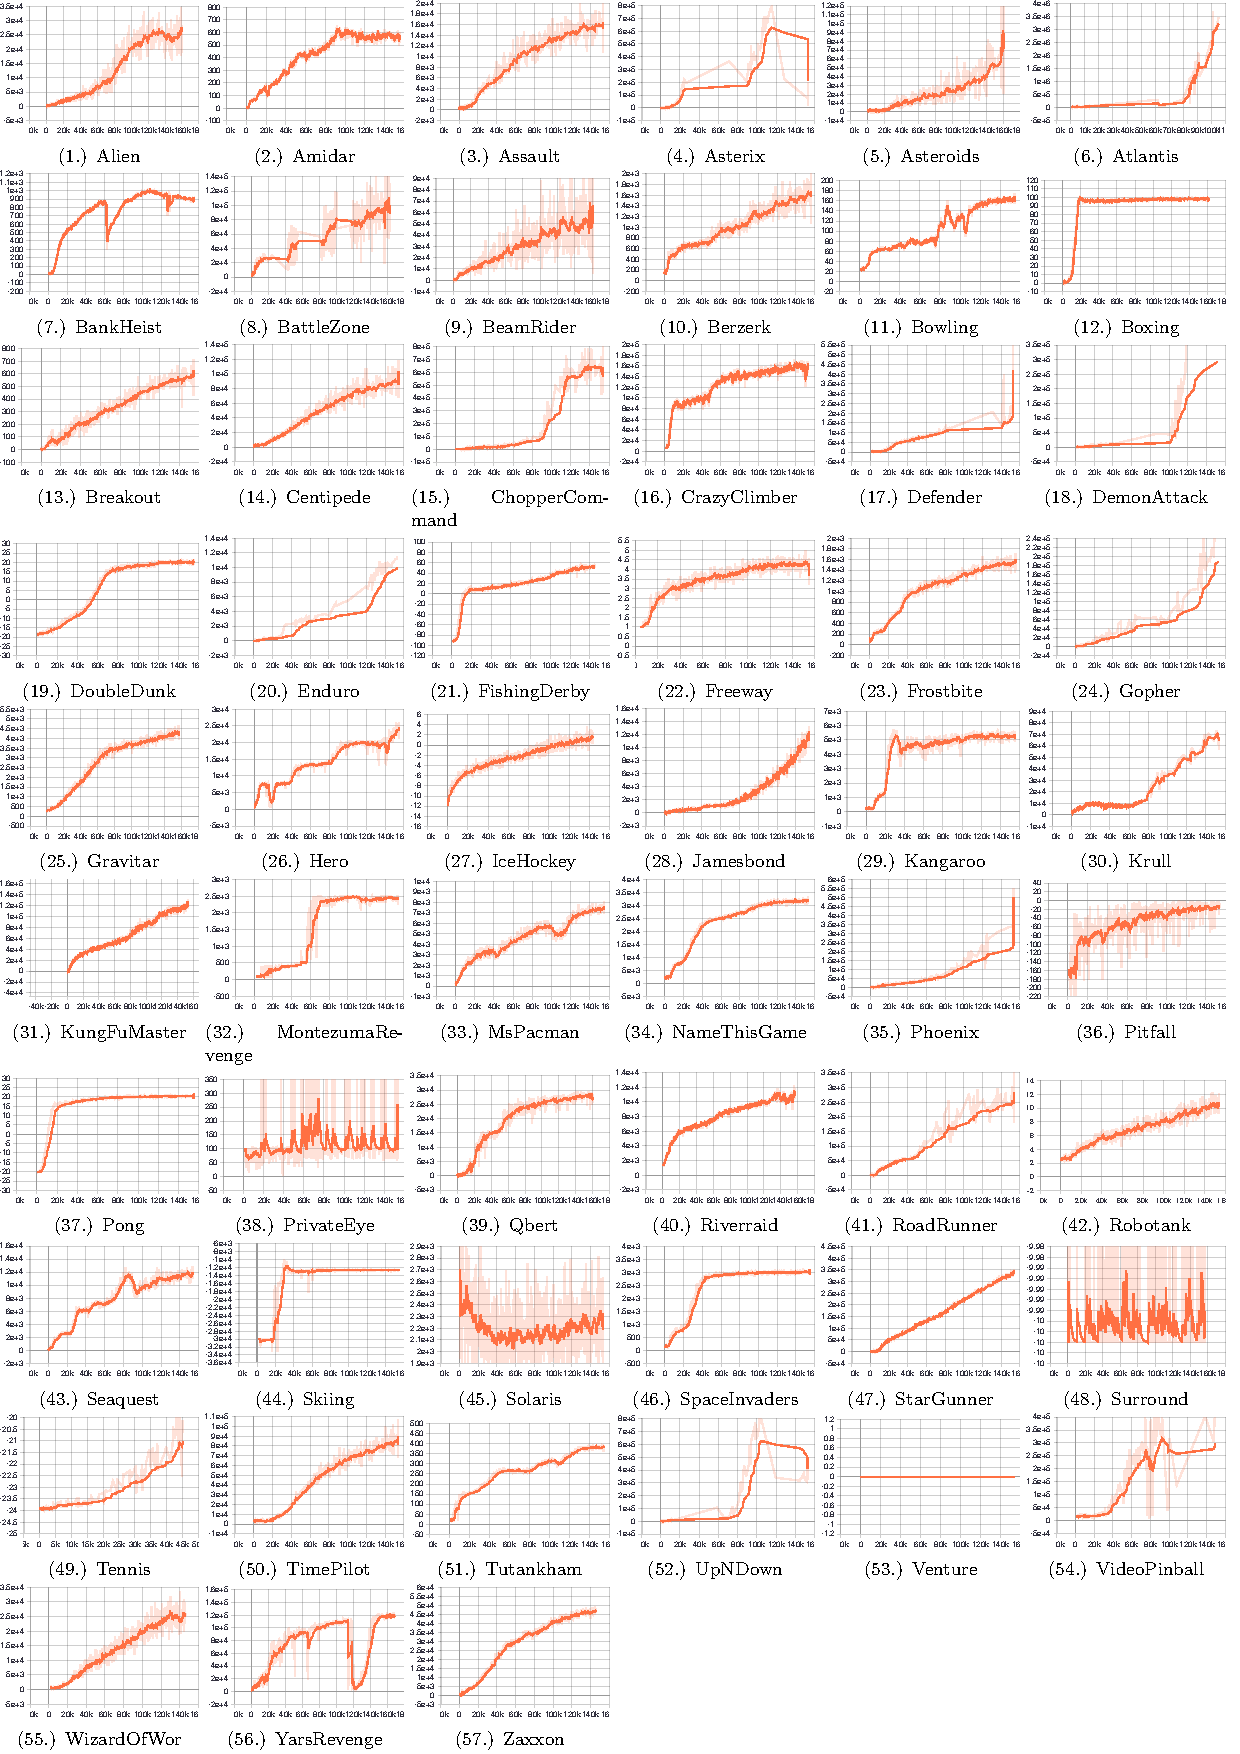
\includegraphics[width=1.0\linewidth]{body/all_fig3.pdf}
\end{figure*}

\clearpage



\end{document}
